% Options for packages loaded elsewhere
\PassOptionsToPackage{unicode}{hyperref}
\PassOptionsToPackage{hyphens}{url}
%
\documentclass[
]{book}
\usepackage{amsmath,amssymb}
\usepackage{lmodern}
\usepackage{ifxetex,ifluatex}
\ifnum 0\ifxetex 1\fi\ifluatex 1\fi=0 % if pdftex
  \usepackage[T1]{fontenc}
  \usepackage[utf8]{inputenc}
  \usepackage{textcomp} % provide euro and other symbols
\else % if luatex or xetex
  \usepackage{unicode-math}
  \defaultfontfeatures{Scale=MatchLowercase}
  \defaultfontfeatures[\rmfamily]{Ligatures=TeX,Scale=1}
\fi
% Use upquote if available, for straight quotes in verbatim environments
\IfFileExists{upquote.sty}{\usepackage{upquote}}{}
\IfFileExists{microtype.sty}{% use microtype if available
  \usepackage[]{microtype}
  \UseMicrotypeSet[protrusion]{basicmath} % disable protrusion for tt fonts
}{}
\makeatletter
\@ifundefined{KOMAClassName}{% if non-KOMA class
  \IfFileExists{parskip.sty}{%
    \usepackage{parskip}
  }{% else
    \setlength{\parindent}{0pt}
    \setlength{\parskip}{6pt plus 2pt minus 1pt}}
}{% if KOMA class
  \KOMAoptions{parskip=half}}
\makeatother
\usepackage{xcolor}
\IfFileExists{xurl.sty}{\usepackage{xurl}}{} % add URL line breaks if available
\IfFileExists{bookmark.sty}{\usepackage{bookmark}}{\usepackage{hyperref}}
\hypersetup{
  pdftitle={Introductory Biostatisics with R},
  pdfauthor={Dylan Z. Childs, Bethan J. Hindle and Philip H. Warren},
  hidelinks,
  pdfcreator={LaTeX via pandoc}}
\urlstyle{same} % disable monospaced font for URLs
\usepackage{color}
\usepackage{fancyvrb}
\newcommand{\VerbBar}{|}
\newcommand{\VERB}{\Verb[commandchars=\\\{\}]}
\DefineVerbatimEnvironment{Highlighting}{Verbatim}{commandchars=\\\{\}}
% Add ',fontsize=\small' for more characters per line
\usepackage{framed}
\definecolor{shadecolor}{RGB}{248,248,248}
\newenvironment{Shaded}{\begin{snugshade}}{\end{snugshade}}
\newcommand{\AlertTok}[1]{\textcolor[rgb]{0.94,0.16,0.16}{#1}}
\newcommand{\AnnotationTok}[1]{\textcolor[rgb]{0.56,0.35,0.01}{\textbf{\textit{#1}}}}
\newcommand{\AttributeTok}[1]{\textcolor[rgb]{0.77,0.63,0.00}{#1}}
\newcommand{\BaseNTok}[1]{\textcolor[rgb]{0.00,0.00,0.81}{#1}}
\newcommand{\BuiltInTok}[1]{#1}
\newcommand{\CharTok}[1]{\textcolor[rgb]{0.31,0.60,0.02}{#1}}
\newcommand{\CommentTok}[1]{\textcolor[rgb]{0.56,0.35,0.01}{\textit{#1}}}
\newcommand{\CommentVarTok}[1]{\textcolor[rgb]{0.56,0.35,0.01}{\textbf{\textit{#1}}}}
\newcommand{\ConstantTok}[1]{\textcolor[rgb]{0.00,0.00,0.00}{#1}}
\newcommand{\ControlFlowTok}[1]{\textcolor[rgb]{0.13,0.29,0.53}{\textbf{#1}}}
\newcommand{\DataTypeTok}[1]{\textcolor[rgb]{0.13,0.29,0.53}{#1}}
\newcommand{\DecValTok}[1]{\textcolor[rgb]{0.00,0.00,0.81}{#1}}
\newcommand{\DocumentationTok}[1]{\textcolor[rgb]{0.56,0.35,0.01}{\textbf{\textit{#1}}}}
\newcommand{\ErrorTok}[1]{\textcolor[rgb]{0.64,0.00,0.00}{\textbf{#1}}}
\newcommand{\ExtensionTok}[1]{#1}
\newcommand{\FloatTok}[1]{\textcolor[rgb]{0.00,0.00,0.81}{#1}}
\newcommand{\FunctionTok}[1]{\textcolor[rgb]{0.00,0.00,0.00}{#1}}
\newcommand{\ImportTok}[1]{#1}
\newcommand{\InformationTok}[1]{\textcolor[rgb]{0.56,0.35,0.01}{\textbf{\textit{#1}}}}
\newcommand{\KeywordTok}[1]{\textcolor[rgb]{0.13,0.29,0.53}{\textbf{#1}}}
\newcommand{\NormalTok}[1]{#1}
\newcommand{\OperatorTok}[1]{\textcolor[rgb]{0.81,0.36,0.00}{\textbf{#1}}}
\newcommand{\OtherTok}[1]{\textcolor[rgb]{0.56,0.35,0.01}{#1}}
\newcommand{\PreprocessorTok}[1]{\textcolor[rgb]{0.56,0.35,0.01}{\textit{#1}}}
\newcommand{\RegionMarkerTok}[1]{#1}
\newcommand{\SpecialCharTok}[1]{\textcolor[rgb]{0.00,0.00,0.00}{#1}}
\newcommand{\SpecialStringTok}[1]{\textcolor[rgb]{0.31,0.60,0.02}{#1}}
\newcommand{\StringTok}[1]{\textcolor[rgb]{0.31,0.60,0.02}{#1}}
\newcommand{\VariableTok}[1]{\textcolor[rgb]{0.00,0.00,0.00}{#1}}
\newcommand{\VerbatimStringTok}[1]{\textcolor[rgb]{0.31,0.60,0.02}{#1}}
\newcommand{\WarningTok}[1]{\textcolor[rgb]{0.56,0.35,0.01}{\textbf{\textit{#1}}}}
\usepackage{longtable,booktabs,array}
\usepackage{calc} % for calculating minipage widths
% Correct order of tables after \paragraph or \subparagraph
\usepackage{etoolbox}
\makeatletter
\patchcmd\longtable{\par}{\if@noskipsec\mbox{}\fi\par}{}{}
\makeatother
% Allow footnotes in longtable head/foot
\IfFileExists{footnotehyper.sty}{\usepackage{footnotehyper}}{\usepackage{footnote}}
\makesavenoteenv{longtable}
\usepackage{graphicx}
\makeatletter
\def\maxwidth{\ifdim\Gin@nat@width>\linewidth\linewidth\else\Gin@nat@width\fi}
\def\maxheight{\ifdim\Gin@nat@height>\textheight\textheight\else\Gin@nat@height\fi}
\makeatother
% Scale images if necessary, so that they will not overflow the page
% margins by default, and it is still possible to overwrite the defaults
% using explicit options in \includegraphics[width, height, ...]{}
\setkeys{Gin}{width=\maxwidth,height=\maxheight,keepaspectratio}
% Set default figure placement to htbp
\makeatletter
\def\fps@figure{htbp}
\makeatother
\setlength{\emergencystretch}{3em} % prevent overfull lines
\providecommand{\tightlist}{%
  \setlength{\itemsep}{0pt}\setlength{\parskip}{0pt}}
\setcounter{secnumdepth}{5}
\usepackage{booktabs}

\usepackage{color}
\usepackage{framed}
\setlength{\fboxsep}{.8em}

\newenvironment{greybox}{
  \definecolor{shadecolor}{rgb}{0.95,0.95,0.95}  % grey
  \color{black}
  \begin{shaded}}
 {\end{shaded}}
 
 \newenvironment{infobox}[1]
  {
  \begin{itemize}
  \renewcommand{\labelitemi}{
    \raisebox{-.7\height}[0pt][0pt]{
      {\setkeys{Gin}{width=3em,keepaspectratio}
        \includegraphics{images/#1}}
    }
  }
  \setlength{\fboxsep}{1em}
  \begin{greybox}
  \item
  }
  {
  \end{greybox}
  \end{itemize}
  }

\ifluatex
  \usepackage{selnolig}  % disable illegal ligatures
\fi
\usepackage[]{natbib}
\bibliographystyle{apalike}

\title{Introductory Biostatisics with R}
\author{Dylan Z. Childs, Bethan J. Hindle and Philip H. Warren}
\date{2021-09-22}

\begin{document}
\maketitle

{
\setcounter{tocdepth}{1}
\tableofcontents
}
\hypertarget{course-information-and-overview}{%
\chapter*{Course information and overview}\label{course-information-and-overview}}
\addcontentsline{toc}{chapter}{Course information and overview}

This book provides a self-contained introduction to the analysis of biological data using the R programming language. Topics include principles of experimental design principles of frequentist statistics, simple statistical tests, analysis of variance, regression, analysis of categorical data, and non-parametric statistics.

\hypertarget{why-do-a-data-analysis-course}{%
\section*{Why do a data analysis course?}\label{why-do-a-data-analysis-course}}
\addcontentsline{toc}{section}{Why do a data analysis course?}

To do science yourself, or to understand the science other people do, you need to understand the principles of experimental design, data collection, statistical analysis and scientific presentation. That does not mean becoming a maths wizard or a computer genius. It means knowing how to make sensible decisions about designing studies and collecting data and then interpreting those data correctly. Sometimes the methods required are straightforward, sometimes more complex. You aren't expected to get to grips with all of them, but what we hope to do in the course is to give you a good practical grasp of the core techniques that are widely used in biology. You should then be equipped to use these techniques intelligently and, equally importantly, know when they are inappropriate and when you need to seek help to find the correct way to design or analyse your study.

With some work on your part, you should acquire a set of skills that you can apply in practicals, field courses, and project work. These same skills will almost certainly also be useful in other situations, whether doing biology, or something completely different. We live in a world increasingly flooded with data, and people who know how to make sense of this are in high demand.

\hypertarget{programming-prerequisites}{%
\section*{Programming prerequisites}\label{programming-prerequisites}}
\addcontentsline{toc}{section}{Programming prerequisites}

This book assumes you have used R and RStudio before and that you are comfortable with the material given in the associated \href{https://tuos-bio-data-skills.github.io/intro-eda-book/}{Exploratory Data Analysis with R} book. What follows is a quick summary of what you need to know.

\hypertarget{r-and-rstudio}{%
\subsection*{R and RStudio}\label{r-and-rstudio}}
\addcontentsline{toc}{subsection}{R and RStudio}

R is a programming language designed first and foremost to support \textbf{data analysis}. We use it to carry out all the statistical analyses covered in this book. R is a fully-fledged programming language, meaning that we have to interact with it by writing computer code. Essentially, R sits and waits for instructions in the form of text (R code). A user can type in those instructions, or they can be sent to it from another helper program. This book assumes you have written R code before and know how to `run it' via these two routes.

We strongly recommend that you use a helper program when working with R. We like RStudio. RStudio makes R a more pleasant and productive tool. RStudio provides a Source Code Editor for working with R code. It also provides a visual, point-and-click means of accessing various language-specific features, such as install packages (see below).

\begin{infobox}{warning}

\hypertarget{r-and-rstudio-are-not-the-same-things}{%
\subsubsection*{R and RStudio are not the same things}\label{r-and-rstudio-are-not-the-same-things}}
\addcontentsline{toc}{subsubsection}{R and RStudio are not the same things}

RStudio is a different program from R---it is installed separately and occupies its own place in the Programs menu (Windows PC) or Applications folder (Mac). You can run R without RStudio but you cannot run RStudio without R.

\end{infobox}

\hypertarget{using-packages}{%
\subsection*{Using packages}\label{using-packages}}
\addcontentsline{toc}{subsection}{Using packages}

R packages extend the basic functionality of R so that we can do more with it. They bundle together R code, data, and documentation in a standardised way that makes it easy to use and share with others. This book uses a subset of the \href{https://www.tidyverse.org}{tidyverse} ecosystem of packages:

\begin{itemize}
\tightlist
\item
  The \textbf{readr} package for reading data into R
\item
  The \textbf{dplyr} package for data manipulation
\item
  The \textbf{ggplot2} package for making plots
\end{itemize}

You need to understand R's package system to use these. This means knowing that \textbf{installing} a package and \textbf{loading} the package are different operations. We only have to install a package onto our computer once, but we have to load the package every time we want to use it in a new R session. If that is confusing, revise the \href{https://tuos-bio-data-skills.github.io/intro-eda-book/packages.html}{package system} chapter Exploratory Data Analysis with R book.

Installing a package can be done via the \texttt{install.packages} function, e.g.~use this code to install the \textbf{dplyr} package:

\begin{Shaded}
\begin{Highlighting}[]
\FunctionTok{install.packages}\NormalTok{(}\StringTok{"dplyr"}\NormalTok{)}
\end{Highlighting}
\end{Shaded}

Alternatively, use the simple RStudio menu interface to install packages. This is accessed via the \textbf{Install} button in the packages tab of the lower right window in RStudio. Loading and attaching a package so that it can be used in a given session happens via the \texttt{library} function, e.g.

\begin{Shaded}
\begin{Highlighting}[]
\FunctionTok{library}\NormalTok{(}\StringTok{"dplyr"}\NormalTok{)}
\end{Highlighting}
\end{Shaded}

\begin{infobox}{warning}

\hypertarget{what-goes-in-your-script}{%
\subsubsection*{What goes in your script?}\label{what-goes-in-your-script}}
\addcontentsline{toc}{subsubsection}{What goes in your script?}

We should not routinely leave \texttt{install.packages} lines in our scripts. Why? Because we don't usually need to install a package every time we run a script---installing packages is a slow `do once' operation. We do usually place one or more \texttt{library} lines at the start of a script to ensure the required packages available in the current R session every time we run the script.

\end{infobox}

\hypertarget{working-with-data}{%
\subsection*{Working with data}\label{working-with-data}}
\addcontentsline{toc}{subsection}{Working with data}

All the examples use data sets that are stored in CSV files. You can get these by \href{mailto:d.childs@sheffield.ac.uk}{emailing the lead author}. We assume you know how to use a function like \texttt{read\_csv} from the \textbf{readr} package to get those data into R. Remember, when using \texttt{read\_csv} we end up with a `tibble': the \textbf{tidyverse} version of a data frame. You could also use the base R \texttt{read\_csv} function to read CSV data into a standard base R data frame---the differences don't matter in this book.

Tibbles and data frame are a table-like objects with rows and columns. They collect together different variables, storing each of them as a named column. We always assume that the data inside these objects are organised according to \href{http://vita.had.co.nz/papers/tidy-data.pdf}{tidy data} conventions. Tidy data has a specific structure that makes it easy to manipulate, model and visualise. A tidy data set is one where each variable is only found in one column, and each row contains one unique observation.

\hypertarget{data-wrangling-with-dplyr}{%
\subsection*{\texorpdfstring{Data wrangling with \textbf{dplyr}}{Data wrangling with dplyr}}\label{data-wrangling-with-dplyr}}
\addcontentsline{toc}{subsection}{Data wrangling with \textbf{dplyr}}

We assume you know how to manipulate data frames and tibbles using the \textbf{dplyr} package. The \textbf{dplyr} package makes it easy to manipulate `rectangular data' that lives in tibbles and data frames. \textbf{dplyr} is orientated around a few core functions, each designed to do one thing well. These \textbf{dplyr} functions are sometimes referred to as its `verbs' to reflect the fact that they `do something' to data. For example:

\begin{itemize}
\tightlist
\item
  \texttt{select} obtains a subset of variables,
\item
  \texttt{mutate} constructs new variables,
\item
  \texttt{filter} obtains a subset of rows,
\item
  \texttt{arrange} reorders rows, and
\item
  \texttt{summarise} calculates information about groups.
\end{itemize}

Notice that the names are chosen to reflect what each function does to the input data. We'll routinely use these---along with a few additional functions such as \texttt{rename} and \texttt{group\_by}---to create new variables, subset data based on some criteria, and calculate summaries for different subsets of data.

\hypertarget{plotting-with-ggplot2}{%
\subsection*{\texorpdfstring{Plotting with \textbf{ggplot2}}{Plotting with ggplot2}}\label{plotting-with-ggplot2}}
\addcontentsline{toc}{subsection}{Plotting with \textbf{ggplot2}}

We assume you know how to create data visualisations using the \textbf{ggplot2} package. A visualisation is created by defining one or more layers, where each layer is associated with some data and a set of rules for how to display the data. We assume you know how to use the \textbf{ggplot2} `grammar' to set up:

\begin{enumerate}
\def\labelenumi{\arabic{enumi})}
\tightlist
\item
  one or more \textbf{layers},
\item
  a set of \textbf{scales},
\item
  a \textbf{coordinate system}, and
\item
  a \textbf{facet} specification for multi-panel plots (optional).
\end{enumerate}

We assume you know how to make basic plots to aid exploratory data analysis. You should be able to:

\begin{itemize}
\tightlist
\item
  visualise single-variable distributions using dot plots and histograms (numeric variables) and bar plots (categorical variables);
\item
  visualise associations between pairs of variables using scatter plots (numeric vs numeric), bar plots (categorical vs categorical), and box plots (numeric vs categorical).
\end{itemize}

We also assume you know how to make more informative plots by defining additional aesthetic mappings (e.g.~\texttt{colour} and \texttt{fill}), or using faceting to construct a multi-panel plot according to the values of categorical variables.

\begin{infobox}{information}

\hypertarget{a-dplyr-cheat-sheet}{%
\subsubsection*{\texorpdfstring{A \textbf{dplyr} cheat sheet}{A dplyr cheat sheet}}\label{a-dplyr-cheat-sheet}}
\addcontentsline{toc}{subsubsection}{A \textbf{dplyr} cheat sheet}

The developers of RStudio have produced very usable \href{http://www.rstudio.com/resources/cheatsheets/}{cheat sheats} that summarise the core packages in the \textbf{tidyverse} ecosystem.

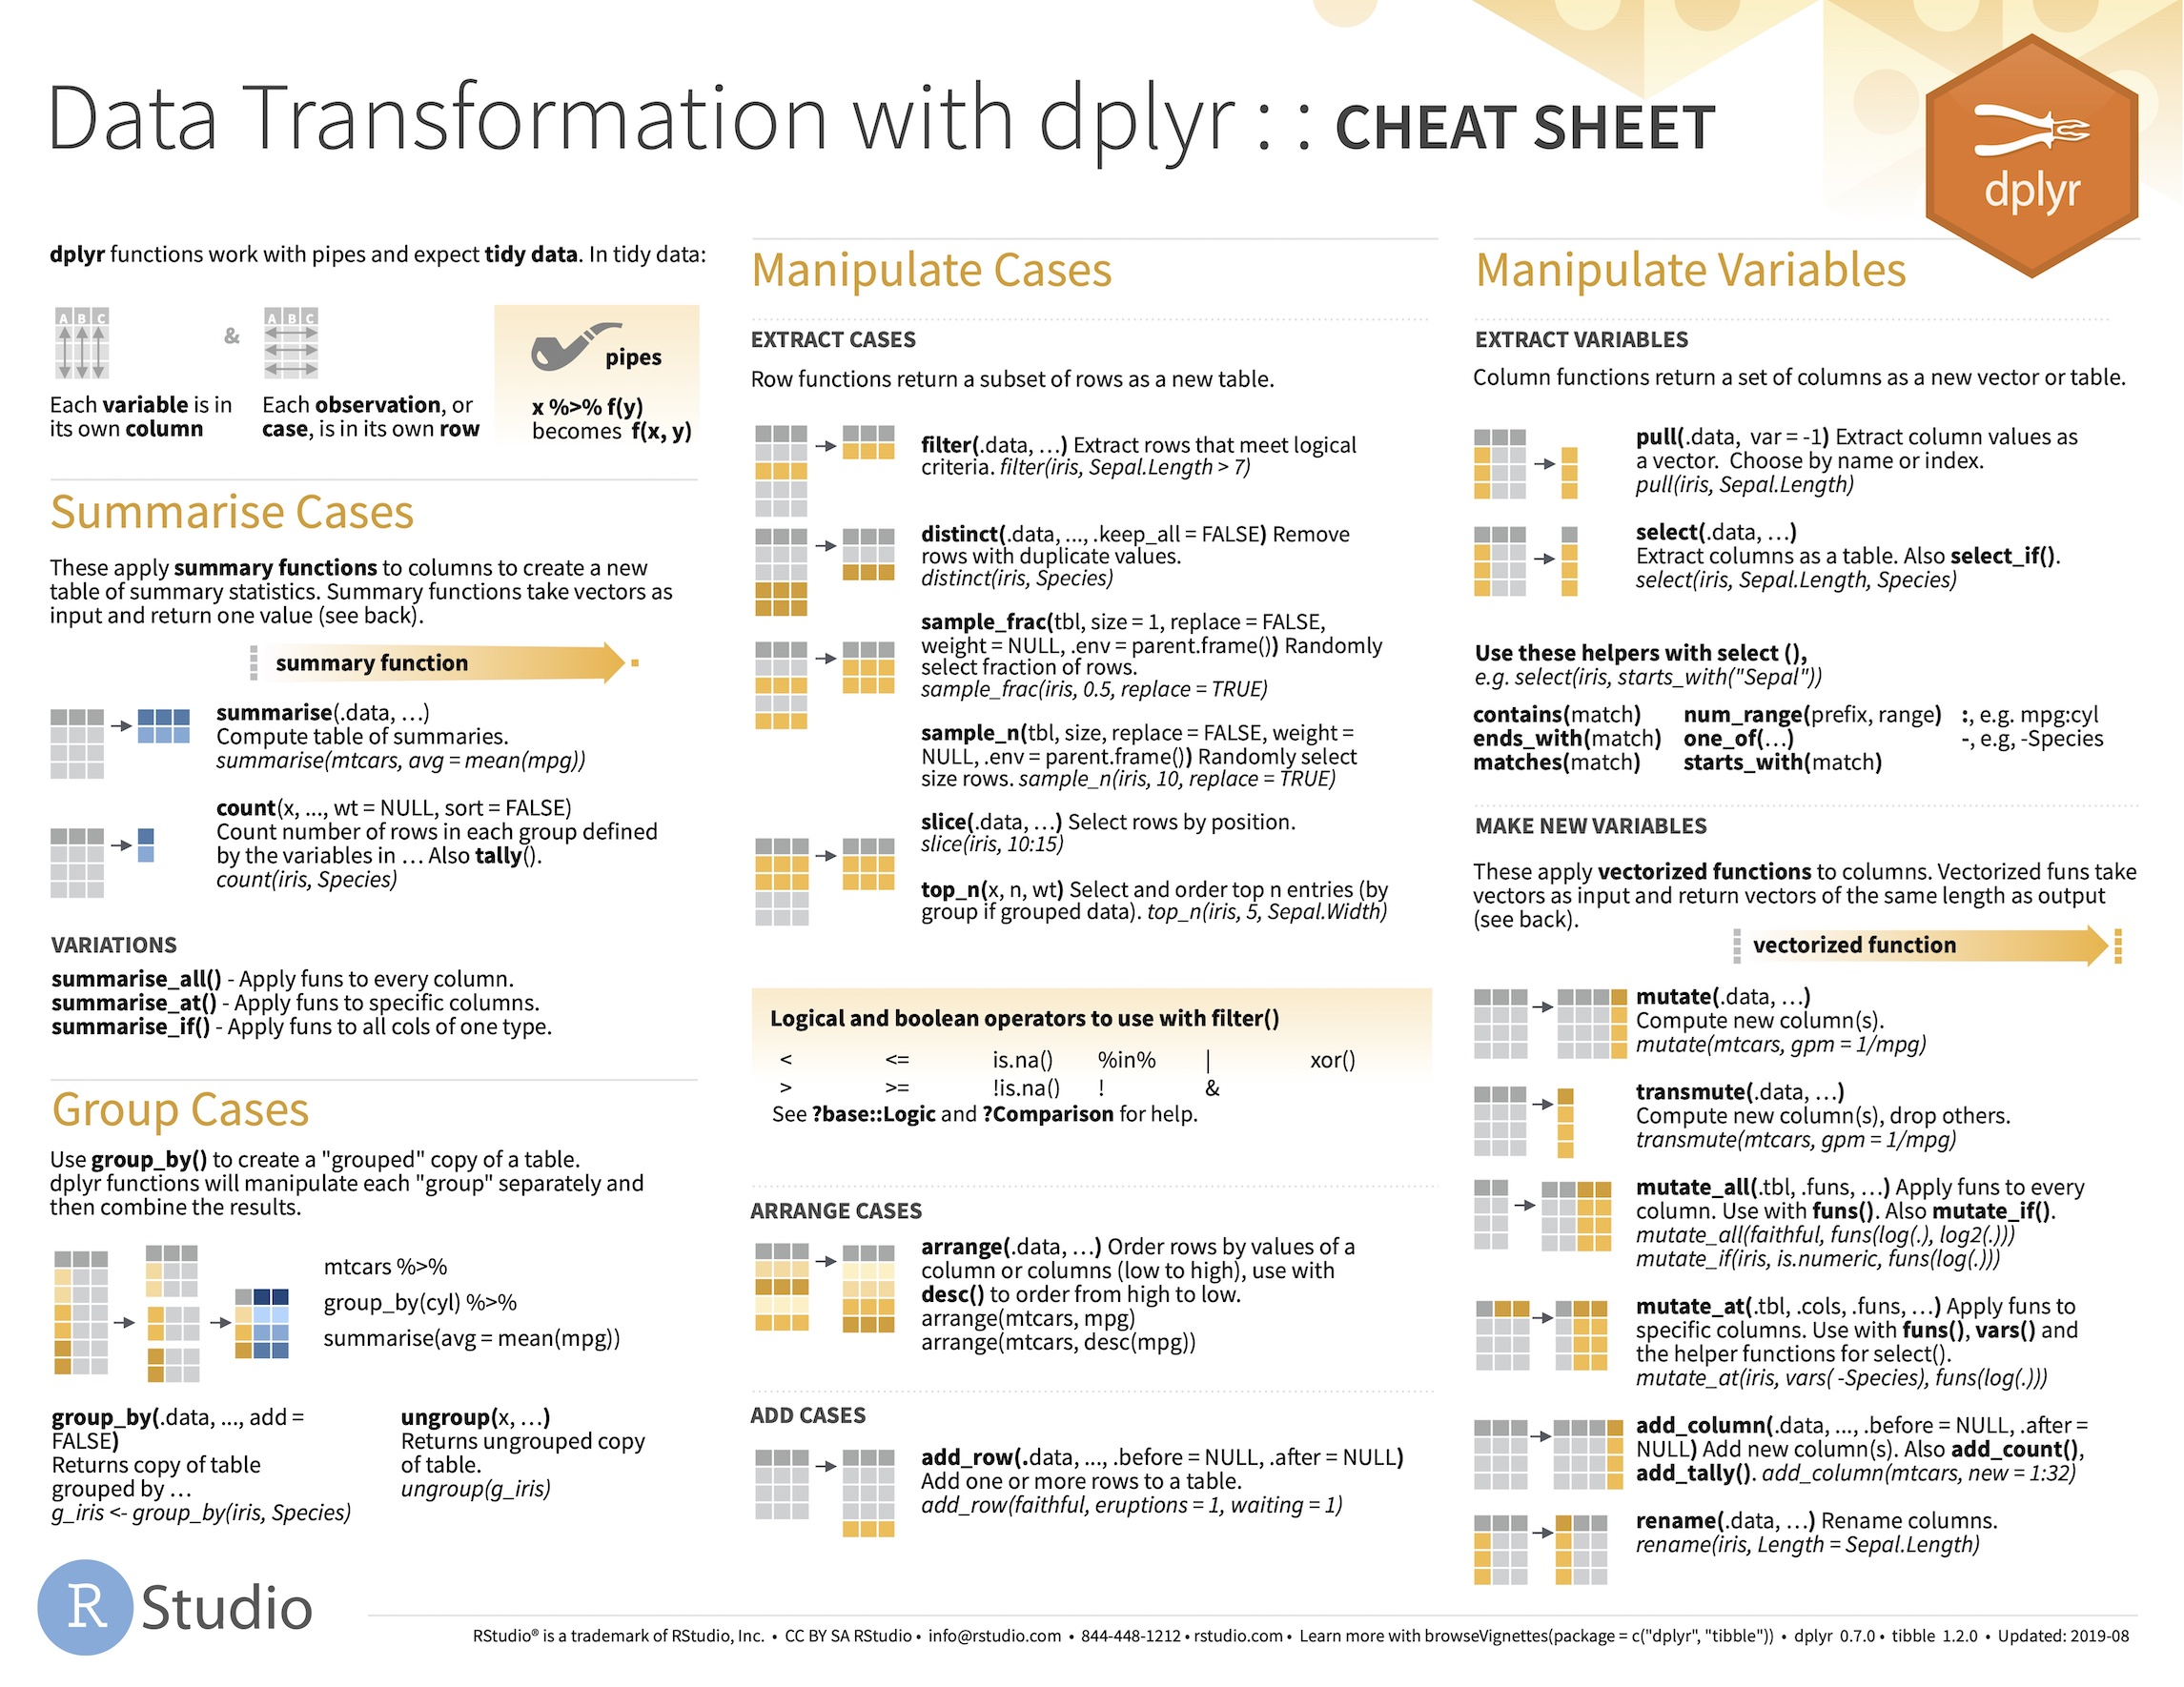
\includegraphics{images/data-transformation.jpg}

Download these, print out a copy, and refer to it when you need to do something with \textbf{dplyr} or \textbf{ggplot2}.

\end{infobox}

\hypertarget{how-the-book-is-formatted}{%
\section*{How the book is formatted}\label{how-the-book-is-formatted}}
\addcontentsline{toc}{section}{How the book is formatted}

We have adopted several formatting conventions in this book to distinguish between normal text, R code, file names, and so on. You need to be aware to make best use of the book.

\hypertarget{text-instructions-and-explanations}{%
\subsection*{Text, instructions, and explanations}\label{text-instructions-and-explanations}}
\addcontentsline{toc}{subsection}{Text, instructions, and explanations}

Normal text---instructions, explanations and so on---are written in the same type as this document. We will tend to use bold for emphasis and italics to highlight specific technical terms when they are first introduced. In addition:

\begin{itemize}
\tightlist
\item
  \texttt{This\ typeface} is used to distinguish R code within a sentence of text: e.g.~``We use the \texttt{mutate} function to change or add new variables.''
\item
  A sequence of selections from an RStudio menu is indicated as follows: e.g.~\textbf{File ▶ New File ▶ R Script}
\item
  File names referred to in the general text are given in upper case in the normal typeface: e.g.~MYFILE.CSV.
\end{itemize}

At various points, you will come across text in different coloured boxes. These are designed to highlight stand-alone exercises or little pieces of supplementary information that might otherwise break the flow. There are three different kinds of boxes:

\begin{infobox}{action}

\hypertarget{action}{%
\subsubsection*{Action!}\label{action}}
\addcontentsline{toc}{subsubsection}{Action!}

This is an \textbf{action} box. We use these when we want you to do something. Do not ignore these boxes.

\end{infobox}

\begin{infobox}{information}

\hypertarget{information}{%
\subsubsection*{Information!}\label{information}}
\addcontentsline{toc}{subsubsection}{Information!}

This is an \textbf{information} box. These aim to offer a discussion of why something works the way it does.

\end{infobox}

\begin{infobox}{warning}

\hypertarget{warning}{%
\subsubsection*{Warning!}\label{warning}}
\addcontentsline{toc}{subsubsection}{Warning!}

This is a \textbf{warning} box. These usually highlight a common `gotcha' that might trip up new users.

\end{infobox}

\hypertarget{r-code-and-output}{%
\subsection*{R code and output}\label{r-code-and-output}}
\addcontentsline{toc}{subsection}{R code and output}

We try to illustrate ideas using snippets of real R code where possible. Stand alone snippets are formatted like this:

\begin{Shaded}
\begin{Highlighting}[]
\NormalTok{tmp }\OtherTok{\textless{}{-}} \DecValTok{1}
\FunctionTok{print}\NormalTok{(tmp)}
\end{Highlighting}
\end{Shaded}

\begin{verbatim}
## [1] 1
\end{verbatim}

The lines that start with \texttt{\#\#} show us what R prints to the screen after it evaluates some R code; they show the output. The lines that~\textbf{do not}~start with \texttt{\#\#} show us the R code; they show us the input. So remember, the absence of \texttt{\#\#} shows us what we are asking R to do. Otherwise, we are looking at something R prints in response to these instructions.

\hypertarget{programming-prerequisites-1}{%
\chapter*{Programming prerequisites}\label{programming-prerequisites-1}}
\addcontentsline{toc}{chapter}{Programming prerequisites}

This chapter gives a quick overview of the prerequisite R skills needed to use this book. These are covered in the \href{https://dzchilds.github.io/eda-for-bio}{Introduction to Exploratory Data Analysis with R} course. We assume you are comfortable using these skills, so you may need to revise them if you feel that you're a little rusty.

\hypertarget{starting-a-learnr-tutorial}{%
\section{\texorpdfstring{Starting a \textbf{learnr} tutorial}{Starting a learnr tutorial}}\label{starting-a-learnr-tutorial}}

You will be using \textbf{learnr} tutorials to gain practical experience of what you learn each week. These interactive tutorials contain three main components:

1 - \textbf{Static Text}: This provides background information for revision purposes or instructions to do something.

2 - \textbf{Code boxes}: These interactive boxes allow you to execute R code and see the results.

3 - \textbf{Quizzes}: These are multiple-choice/multiple-answer questions designed to check your understanding.

You will be given a visual `walk-through' of running a \textbf{learnr} tutorial in week one of the course. The first tutorial aims to be self-describing---it provides a stand-alone introduction to how to use the tutorials.

\hypertarget{using-packages-1}{%
\section{Using packages}\label{using-packages-1}}

R packages extend the basic functionality of R so that we can do more with it. In a nutshell, an R package bundles together R code, data, and documentation in a standardised way that is easy to use and share with other users. This book uses a subset of the \href{https://www.tidyverse.org}{tidyverse} ecosystem of packages:

\begin{itemize}
\tightlist
\item
  The readr package for reading data into R
\item
  The dplyr package for data manipulation
\item
  The ggplot2 package for making plots
\end{itemize}

We need to understand how R's package system works to use these. Here's the key point: \textbf{installing} a package and \textbf{loading} the package are different operations. We only have to install a package onto our computer once but we have to load and attach the package every time we want to use it in a new R session (i.e.~every time we start RStudio). If that is confusing, revise the \href{https://dzchilds.github.io/eda-for-bio/packages.html}{package system} chapter Exploratory Data Analysis in R book.

Installing a package can be done via the \texttt{install.packages} function, e.g.~use this code to install the \textbf{dplyr} package:

\begin{Shaded}
\begin{Highlighting}[]
\FunctionTok{install.packages}\NormalTok{(}\StringTok{"dplyr"}\NormalTok{)}
\end{Highlighting}
\end{Shaded}

Alternatively, you can use RStudio's menu interface via the packages tab in the bottom right window.

Either way is fine. However, the \texttt{install.packages} route should be carried by typing the install commands directly into the Console (this is pretty much the only time we work this way). \textbf{Do not leave \texttt{install.packages} statements in your R scripts.} We only have to install a package once onto our computer to make it available. Because installing packages can be slow, we'd rather not do that every time we have to run a script.

Loading and attaching a package so that it can actually be used happens via the \texttt{library} function, e.g.

\begin{Shaded}
\begin{Highlighting}[]
\FunctionTok{library}\NormalTok{(}\StringTok{"dplyr"}\NormalTok{)}
\end{Highlighting}
\end{Shaded}

People usually place \texttt{library} statements at the beginning of scripts to ensure that all the package functions they need are available to the rest of the script.

\hypertarget{reading-data-into-r}{%
\section{Reading data into R}\label{reading-data-into-r}}

Last year we made extensive use of `built in' data sets that reside inside R. This meant we could use the data without getting bogged down trying to read it into R. We'll carry on doing that at times as we work through the book and the accompanying \textbf{learnr} tutorials. However, we don't have the luxury of this short cut when we work with our own data, so we'll work towards adopting more realistic practices as we go.

In `real world' data analysis, when we need to work with data, we typically save a copy of it into some kind of file on our computer and then read that file into R. The data sets we use in this course are stored as a Comma Separated Value (`CSV') text files. The base R \texttt{read.csv} or the \texttt{read\_csv} function from the \textbf{readr} package can be used to read in such files.

If we use \texttt{read.csv} the resulting R data object is a data frame. If we use \texttt{read\_csv} we end up with a `tibble' which can be thought of as the tidyverse version of a data frame. Either is fine, the differences don't matter in this book. A data frame is a table-like object that collects together different variables, storing each of them as a named column. We can access the data inside the data frame by referring to particular columns and rows, or manipulate the whole data frame with a package like \textbf{dplyr}.

If that last paragraph was confusing, it would be a good idea to work through the \href{https://dzchilds.github.io/eda-for-bio/data-frames.html}{data frames} chapter of the Exploratory Data Analysis in R book.

\hypertarget{part-collecting-and-using-data}{%
\part{Collecting and Using Data}\label{part-collecting-and-using-data}}

\hypertarget{scientific-process}{%
\chapter{The scientific process}\label{scientific-process}}

\begin{quote}
\emph{There is something fascinating about science. One gets such a wholesale return of conjecture out of a trifling investment of fact.}

Mark Twain

\emph{To do science is to search for patterns, not simply to accumulate facts.}

Robert MacArthur
\end{quote}

\hypertarget{stages-scientific-process}{%
\section{Stages in the scientific process}\label{stages-scientific-process}}

Science is about asking, and answering, the right questions. A number of distinct stages occur within this process: making observations, asking questions, formulating hypotheses, and testing predictions. Collectively these are the building blocks of what is known as the scientific method. Exactly how they fit together, and what the philosophical and practical limitations of different approaches are, have been the subject of much debate by philosophers of science. We're not going to tackle those issues here, but instead try to extract a general working framework for the process of a typical scientific investigation.

\hypertarget{stages-observations}{%
\subsection{Observations}\label{stages-observations}}

\textbf{Observation} --- \emph{information, or impression, about events or objects}.

In general the questions we ask are not generated by pure abstract thought, but are a result of observations about the natural world. These may take the form of direct observations we make ourselves, patterns that crop up in data collected for other purposes, in non-specific surveys, and the accumulated works of other people.

Such observations of biological systems will lead almost automatically into asking questions.

\hypertarget{stages-questions}{%
\subsection{Questions}\label{stages-questions}}

\textbf{Question} --- \emph{what it is that you want to know; the scope of your investigation}.

It is important to keep the question sufficiently focussed. The overall aim of a particular study should be to answer one or (perhaps) two questions. The question of why the tropics are more diverse than the temperate regions is a valid and fascinating question, but it's probably not be a good choice for a final year project or even a PhD.

The next stage is to formulate an hypothesis.

\hypertarget{stages-hypotheses}{%
\subsection{Hypotheses}\label{stages-hypotheses}}

\textbf{Hypothesis} --- \emph{an explanation proposed to account for observed facts.}

In general, in biology, the critical distinguishing feature of an hypothesis is that it specifies some biological process, or processes, which might account for the observations made. Formulating hypotheses requires more than just a restatement of the question -- it usually embodies some mechanism (though this may not be fully understood) and it will often draw on additional information. One question will also often generate more than one hypothesis.

Once we have formulated a set of hypotheses, we need to derive the predictions that follow.

\hypertarget{stages-predictions}{%
\subsection{Predictions}\label{stages-predictions}}

\textbf{Prediction} --- \emph{what you would expect to see if the hypothesis was true}.

Hypotheses are about proposing explanations, but they might not be directly testable. That is, they may not tell us what data to collect, or what pattern to expect in the data. To be able to test an hypothesis we need to make some predictions from that hypothesis. These will be determined both by what we expect to see and what it is possible, or practical, to measure. A prediction is not simply a rephrasing of the hypothesis -- it should more or less lead to a statement of the experiment to conduct or observation to make, and type of data to collect.

The ideal prediction is one that is unique to the hypothesis it is based on, so if the prediction is true only one of the hypotheses could have been responsible. It may not always be possible to generate such `clean' predictions, in which case, some combination of predictions may need to be considered. Additionally, several processes may be operating at the same time, which makes hypothesis testing harder still, because it may be necessary to consider two or more hypotheses, and their corresponding predictions, in combination.

Science is hard!

\hypertarget{an-example}{%
\section{An example}\label{an-example}}

\hypertarget{observations}{%
\subsubsection*{Observations}\label{observations}}
\addcontentsline{toc}{subsubsection}{Observations}

Imagine, while observing a stream one day, we notice that the freshwater `shrimps' (\emph{Gammarus}) seem to occur almost entirely under stones; we rarely seem to see them in a patch of open stream bed. Having made observations, it may be necessary to collect some more data to check that this phenomenon is not just a one-off event, or a false impression. Look under a few more stones, watch the same species another day, or in another place, check the literature for similar observations by others.

\hypertarget{question}{%
\subsubsection*{Question}\label{question}}
\addcontentsline{toc}{subsubsection}{Question}

Why does \emph{Gammarus} spend most of its time under stones?

\hypertarget{hypotheses}{%
\subsubsection*{Hypotheses}\label{hypotheses}}
\addcontentsline{toc}{subsubsection}{Hypotheses}

\emph{Gammarus} occur under stones because:

\begin{itemize}
\item
  they need to shelter from the current
\item
  their food (leaf litter) gets trapped and accumulates under stones
\item
  they are subject to predation by visually hunting fish and need to remain out of sight
\end{itemize}

\hypertarget{predictions}{%
\subsubsection*{Predictions}\label{predictions}}
\addcontentsline{toc}{subsubsection}{Predictions}

Taking each hypothesis in turn, we expect to observe:

\begin{itemize}
\item
  \emph{Shelter hypothesis:} a greater proportion of \emph{Gammarus} should be found in the open in streams with slow flow, or in slower flowing areas of a stream.
\item
  \emph{Food hypothesis:} \emph{Gammarus} should not aggregate under stones from which all leaf litter has been removed; \emph{Gammarus} should aggregate on patches of leaf litter tethered in the open part of the stream bed.
\item
  \emph{Predation hypothesis:} \emph{Gammarus} should aggregate under stones more in streams where fish are present than where they are not; \emph{Gammarus} may spend less time under stones at night.
\end{itemize}

If we want to tease apart our hypotheses we may need to refine these predictions. For example, \emph{Gammarus} may be under stones because it prefers the sheltered environment, but also because food accumulates there. In this case we might expect that \emph{Gammarus} will show a weak aggregative response to shelter alone, or food alone, and a stronger one to them both together.

\hypertarget{hypothesis-testing}{%
\section{Hypothesis testing}\label{hypothesis-testing}}

Once we have firmed up our hypotheses and predictions we are in the position to collect data to evaluate our ideas. On the basis of these data we will either accept or reject our various hypotheses. The important thing to realise about the process of hypothesis testing is that, in science especially, hypotheses are either rejected, or not rejected, but an hypothesis can rarely, except in trivial cases, be proved.

Why is this? Since we cannot be sure that we've thought of all the possible hypotheses to explain an observation, finding evidence that supports a prediction does not guarantee that the underlying hypothesis is the only one which could have produced the effect we find. On the other hand, if we find evidence that directly contradicts the prediction(s) from an hypothesis, we can be certain (assuming the prediction and data are not flawed) that the hypothesis cannot be true.

An hypothesis which predicted that all conifers should be evergreen could be supported by numerous observations of different conifer species in forests around the world, but is conclusively refuted by the first larch tree we encounter.

Having tested our hypothesis, by examining the evidence that its predictions are true, we may accept it as the best current explanation of the observations, or we may reject it as an explanation, and turn to other hypotheses. The same procedure must then be repeated for these hypotheses.

This basic cycle of proposing hypotheses and then seeking evidence potentially capable of falsifying them, is, in essence, the idealized model of the scientific process famously proposed by the philosopher of science Karl Popper (1902-1994). It is often termed \emph{falsificationism}.

\hypertarget{are-we-sure}{%
\section{Don't we ever know anything for sure?}\label{are-we-sure}}

The method presented here provides a view of science as one in which we suggest hypotheses, then test them, trying to reject them by finding conclusive counter-evidence, then replacing them with new hypotheses. It all sounds a bit frustrating.

In fact of course we do `accept' hypotheses all the time -- that is, we fail to reject them over and over again. These hypotheses become more accepted and in some sense become regarded as `true' if repeated attempts to test them all fail to provide good counter evidence. In other words, we have some ideas that are doing pretty well in terms of resisting falsification, and we use these as our best estimates of the truth, with the proviso that it is still possible a better idea will come along in due course.

The simple process of falsification described above also presents a picture of scientists as neutral, objective creatures, rationally proceeding through cycles of setting up hypotheses, testing them, rejecting them, setting them aside and starting over again. Of course this is not a true reflection of the complex, often messy, business involved in trying to figure out how the world works. Philosophers of science have argued long and hard about how far from this idealized process real science actually is. Various alternative philosophies suggest more `realistic' processes. For example\ldots{}

\begin{itemize}
\item
  Thomas Kuhn's view of science as periods of relative stasis, where people work within an accepted paradigm (a set of views about how things work) despite accumulating evidence that doesn't always support the paradigm, until finally it is upset by a `revolution' which rejects the entire paradigm, and proposes a new view. This is where the phrase `paradigm shift' originated.
\item
  Imre Lakatos proposed some resolution of Kuhn's views, suggesting that scientific ideas were grouped together in `research programmes' concerned with particular endeavours, and that within these there may be core ideas that are not challenged, but other related ideas that are being challenged and adjusted by falsification, and that together these make each research programme progress.
\end{itemize}

This is a very over-simplified sketch of some important ideas. These are well worth reading about, but in practice most philosophical arguments are more focused on how whole areas of science develop. When thinking about how to construct a study of one problem, the basic falsification cycle is a pretty good approach to have in mind. Keep in mind that the process laid out here is not a strict set of rules, but outlines an approach to scientific investigation which is widely considered to provide a rigorous and productive system. As with all such systems understanding the `normal' process is a prerequisite for constructively breaking the rules.

\hypertarget{data-variables}{%
\chapter{Data and variables}\label{data-variables}}

\begin{quote}
\emph{The truth is the science of nature has been already too long made only a work of the Brain and the Fancy. It is now high time that it should return to the plainness and soundness of Observations on material and obvious things.}

Robert Hooke (1665)

\emph{The plural of anecdote is not data.}

Roger Brinner
\end{quote}

\hypertarget{observations-on-material-and-obvious-things}{%
\section{``Observations on material and obvious things''}\label{observations-on-material-and-obvious-things}}

As Hooke's observation suggests, science cannot proceed on theory alone. The information we gather about a system stimulates questions and ideas about it and, in turn, can also allow us to test these ideas. In fact, the idea of measuring and counting things is so familiar that it is easy to start a project without giving much thought to something as mundane as the nature, quantity and resolution of the data we intend to collect. Nonetheless, the features of the data we collect determine the types of analyses that can be carried out and the confidence we can have in the conclusions drawn. In the end, no level of analytical sophistication will enable us to extract information that is not there to begin with.

So what is there to say about data? The first point to note is that there are many different sorts of data. We focus on simple kinds of data in this book, such as quantities (`how much') or classifications (`what kind'), but not everything can be thought of in simple terms. Examples of more complex data types include spatial maps of species' occurrence, the DNA sequences of individuals, and networks of feeding relationships among species (i.e.~food webs) or gene activation (gene regulatory networks).

The data we collect in a study can be organised into one or more statistical \textbf{variables}. In its loosest sense, statisticians use the word `variable' to mean any characteristic measured or experimentally controlled on different items or objects. People tend to think of variables as numeric quantities, such as cell size, but nothing stops us working with non-numeric variables, such as developmental stage.

Collectively, a set of related variables is referred to as a \textbf{data set} (or just `the data'). Confused? Consider a concrete example: the spatial maps of species' occurrence mentioned above. A minimal data set might comprise two variables containing the x and y position of sample locations, a third variable denoting the presence/absence of a species, and one or more additional variables containing information about the environmental factors we measured.

\begin{infobox}{information}
\textbf{Data and variables in R}

Data sets are often stored in data frames when working with R. A data frame can be thought of as having rows and columns. Each column in a data frame has to be one of R's many types of `vector'. Typically, these are simple things, like numeric or character vectors, but other kinds of vector can be used (e.g.~dates and intervals of times). The data it contains are said to be \href{https://cran.r-project.org/web/packages/tidyr/vignettes/tidy-data.html}{tidy} when each column of a data frame corresponds to a statistical variable, and each row corresponds to a single observation (a cell, a tissue sample, an animal, etc).

This simple connection between abstract statistical concepts and concrete objects in R is not a coincidence. Its structures and abstractions reflect the fact that R was designed first and foremost to analyse data.

\end{infobox}

\begin{infobox}{information}
\textbf{The data are or the data is?}

Strictly speaking, the word data is the plural of datum (a single piece of information), so we should say ``the data are\ldots{}'' not ``the data is\ldots{}''. That said, the use of the word in the singular has become widespread, despite the objections of \href{http://www.urbandictionary.com/define.php?term=Grammar\%20Nazi}{Grammar Nazis}, and to be perfectly honest, either usage is fine these days. We lean towards plural usage with `data', but both forms appear in this book\ldots{}

\end{infobox}

\hypertarget{var-types}{%
\section{Revision: Types of variable}\label{var-types}}

When designing an experiment or carrying out some data analysis, it is vital to understand what sort of data we need, or have, as this affects what we can do with it. The variables in a data set are often classified as being either \textbf{numeric} or \textbf{categorical}:

\begin{itemize}
\tightlist
\item
  Numeric variables have values that describe a measurable quantity as a number, like `how many' or `how much'.
\item
  Categorical variables have values that describe a characteristic of an observation, like `what type' or `which category'.
\end{itemize}

Numeric variables can be further characterised according to the type of scale they are measured on: \textbf{interval} vs.~\textbf{ratio} scales. Categorical variables can be further characterised according to whether or not they have a natural order: \textbf{nominal} vs.~\textbf{ordinal} variables.

This is probably the minimal classification scheme we need to learn if we want to analyse our data well. Let's take a closer look at this scheme.

\hypertarget{nominal-categorical-variables}{%
\subsection{Nominal (categorical) variables}\label{nominal-categorical-variables}}

Nominal variables arise when observations are recorded as categories that have no natural ordering relative to one other. For example:

\begin{longtable}[]{@{}ccc@{}}
\toprule
& & \\
\midrule
\endhead
\textbf{Marital status} & \textbf{Sex} & \textbf{Colour morph} \\
Single & Male & Red \\
Married & Female & Yellow \\
Widowed & & Black \\
Divorced & & \\
\bottomrule
\end{longtable}

Variables of this type are common in surveys where, for example, a record is made of the `type of thing' (e.g.~the species) observed.

\hypertarget{ordinal-categorical-data}{%
\subsection{Ordinal (categorical) data}\label{ordinal-categorical-data}}

Ordinal variables occur where observations can be assigned some meaningful order but the exact `distance' between items is not fixed, or even known. For example, if we are studying the behaviour of an animal when it meets a conspecific, it may not be possible to obtain quantitative data about the interaction, but we might be able to score the behaviours in order of aggressiveness:

\begin{longtable}[]{@{}lc@{}}
\toprule
& \\
\midrule
\endhead
\textbf{Behaviour} & \textbf{Score} \\
initiates attack & 3 \\
aggressive display & 2 \\
ignores & 1 \\
retreats & 0 \\
\bottomrule
\end{longtable}

Rank orderings are a type of ordinal data. For example, the order in which runners finish a race (1st, 2nd, 3rd, etc.) is a rank ordering. It doesn't tell us whether it was a close finish or not but still conveys important information about the result.

In both situations, we can say something about the relationships between categories: in the first example, the larger the score, the more aggressive the response; in the second example, the greater the rank, the slower the runner. However, we can't say that the gap between the first runner and the second was the same as between the second and third and we can't say that a score of 2 is twice as aggressive as a score of 1.

\begin{infobox}{warning}
\textbf{How should you encode different categories in R?}

We always have to define a coding scheme to represent the categories of nominal/ordinal variables in computerised form. It was once common to assign numbers to different categories (e.g.~Female=1, Male=2). This method was sensible in the early days of computer-based analysis because it allowed data to be stored efficiently. This efficiency argument is no longer relevant. What's more, there are good \emph{practical} reasons to avoid coding categorical variables as numbers:

\begin{itemize}
\item
  Numeric coding makes it harder to understand our raw data and interpret the output of a statistical analysis of those data. This is because we have to remember which number is associated with each category.
\item
  Numeric codes are arbitrary and should not be used as numbers in mathematical operations. In the above example, it is meaningless to say 2 {[}``male''{]} is twice the size of 1 {[}``female''{]}.
\end{itemize}

R usually assumes that a variable containing numeric values is meant to be treated as a number. If we use numeric coding for a categorical variable, R will try to treat the offending variable as a number, leading to confusing errors.

The take home message: Always use words (e.g., `female' vs.~`male'), not numbers, to describe categories in R.

\end{infobox}

\hypertarget{ratio-scale-numeric-variables}{%
\subsection{Ratio scale (numeric) variables}\label{ratio-scale-numeric-variables}}

Ratio scale numeric variables have a true zero and a known and consistent mathematical relationship between any points on the measurement scale. For example, there is a temperature scale that has a true zero: the Kelvin scale. Zero K is absolute zero, where matter has no thermal energy whatsoever. Temperature measurements in degrees K are on a ratio scale, i.e.~it \textbf{does} make sense to say that 60 K is twice as hot as 30 K. Ratio scale numeric variables are quite familiar, because the physical quantities that crop up in science are usually measured on a ratio scale: length, weight, and numbers of objects are good examples.

\hypertarget{interval-scale-numeric-variables}{%
\subsection{Interval scale (numeric) variables}\label{interval-scale-numeric-variables}}

Interval scale variables take values on a consistent numeric scale, but where that scale starts at an arbitrary point. Differences between values on an interval scale are meaningful, whereas ratios are not. The temperature on the Celsius scale is a good example of interval data. We can say that 60º C is hotter than 50º C, and we can say that the difference in temperature between 60º C and 70º C is the same as that between -20º C and -10º C. We cannot say that 60º C is twice as hot as 30º C. This is because temperature on the Celsius scale has an artificial zero value---the freezing point of water. The idea becomes obvious when we consider that temperature can equally well be measured on the Fahrenheit scale (where the freezing point of water is 32º F).

\begin{infobox}{information}
\textbf{Continuous or discrete?}

A common confusion with numeric data concerns whether the data are on continuous or discrete scales. Many biological ratio data are discrete (i.e.~only certain discrete values are possible in the original data). Count data are an obvious example, e.g.~the number of eggs found in a nest, the number of mutations in a cancer cell, or the number of heartbeats counted in a minute. These can only comprise whole numbers, `in between' values are not possible.

However, the distinction between continuous and discrete data is often not clear cut -- even `continuous' variables such as weight are made discrete in reality by the fact that our measuring apparatus is of limited resolution (i.e.~a balance may weigh to the nearest 0.01 g). So\ldots{} keep in mind that the fact that data look (or really are) discrete does not mean they are necessarily truly discrete data.

\end{infobox}

\hypertarget{why-does-the-distinction-matter}{%
\subsection{Why does the distinction matter?}\label{why-does-the-distinction-matter}}

The measurement scale affects what we can do mathematically to a numeric variable. We can add and subtract interval scale variables, but we can not divide or multiply them and arrive a meaningful result. In contrast, we can add, subtract, multiply or divide ratio scale variables. Put another way, differences and distances are meaningful for both interval and ratio scales, but ratios are only meaningful for ratio variables (yes, the clue is in the name).

\hypertarget{which-is-best}{%
\subsection{Which is best?}\label{which-is-best}}

All types of data can be useful, but it is important to be aware that not all types of data can be used with all statistical models. This is one very good reason for why it is worth having a clear idea of the statistical tools we intend to use when designing a study.

In general, ratio variables are best suited to statistical analysis. However, biological systems often cannot be readily represented as ratio data, or the work involved in collecting good ratio data may be vastly greater than the resources allow, or the question we are interested in may not demand ratio data to achieve a perfectly satisfactory answer. It is this last question that should come first when thinking about a study. What sort of data do we need to answer the question we are interested in? Suppose it is clear at the outset that data on a rank scale will not be sufficiently detailed to enable us to answer the question. In that case, we must either develop a better way of collecting the data, or abandon that approach altogether. If we know the data we're able to collect cannot address the question, we should do something else.

An obvious but important point: we can always convert measurements taken on a ratio scale to an interval scale, but we cannot do the reverse. Similarly, we can convert interval scale data to ordinal data, but we cannot do the reverse. That said, it's good practice to avoid such conversions as they inevitably result in a loss of information.

\hypertarget{accuracy-precision}{%
\section{Accuracy and precision}\label{accuracy-precision}}

\hypertarget{what-do-they-mean}{%
\subsection{What do they mean?}\label{what-do-they-mean}}

The two terms accuracy and precision are used more or less synonymously in everyday speech, but they have quite distinct meanings in scientific investigation.

\textbf{Accuracy} -- how close a measurement is to the true value of whatever it is you are trying to measure.

\textbf{Precision} -- how repeatable a measure is, irrespective of whether it is close to the actual value.

Imagine we are measuring an insect's weight on an old and poorly maintained balance, which measures to the nearest 0.1 g. In that case, we might weigh the same insect several times and each time get a different weight --- the balance is not very precise, though some of the measurements might happen be quite close to the real weight. By contrast, we could be using a new electronic balance, weighing to the nearest 0.01g, but which has been incorrectly zeroed so that it is 0.2 g out from the true weight. Repeated weighing here might yield results that are identical but all incorrect --- the balance is precise, but the results are inaccurate. The analogy often used is with shooting at a target:

\begin{figure}

{\centering 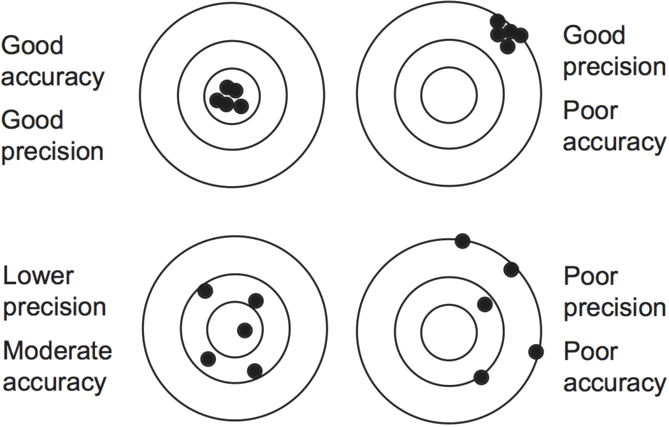
\includegraphics[width=0.6\linewidth]{images/targets} 

}

\caption{Accuracy and precision}\label{fig:targets}
\end{figure}

It's important to know how accurate and how precise our data are. The ideal is the situation in the top left target in the diagram. Still, high precision is not possible in many circumstances, and it is usually preferable to make measurements whose accuracy we can be reasonably confident (bottom left), than more precise measurements, whose accuracy may be suspect (top right). Taking an average of the values for the bottom left target would produce a value pretty close to the centre; taking an average for the top right target wouldn't help the accuracy at all.

\hypertarget{implied-precision-significant-figures}{%
\subsection{Implied precision -- significant figures}\label{implied-precision-significant-figures}}

It's worth being aware that when we state results, we're making implicit statements about the precision of the measurement. The number of significant figures we use suggests something about the precision of the result. A result quoted as 12.375 mm implies the measurement is more precise than one quoted as 12.4 mm. A value of 12.4 actually measured with the same precision as 12.735 should properly be written 12.400. When quoting results, look at the original data to decide how many significant figures to use---generally, the same number of significant figures will be appropriate.

These considerations do not apply in the same way when working with discrete data, e.g.~precision of measurement is not an issue in recording the number of eggs in a nest. We use 4 not 4.0, but since 4 eggs implies 4.0 eggs it's fine to quote average clutch size from several nests as 4.3 eggs. However, even with discrete data, if numbers are large then obviously precision is an issue again \ldots{} a figure of 300 000 ants in a nest is likely to imply a precision of plus or minus 50 000. A figure of 320987 ants implies an improbably precise measurement.

\hypertarget{how-precise-should-measurements-be}{%
\subsection{How precise should measurements be?}\label{how-precise-should-measurements-be}}

The appropriate precision to use when making measurements is largely common sense. It will depend on practicality and the use to which we wish to put the data. It may not be possible to weigh an elephant to the nearest 0.001g, but if we want to know whether the elephant will cause a 10-tonne bridge to collapse, then the nearest tonne will be good enough. On the other hand, if we want to compare the mean sizes of male and female elephants, then the nearest 100 kg may be sufficient, but if we plan to monitor the progress of a pregnant female elephant, then the nearest 10 kg or less might be desirable.

As a rough guide aim, where possible, for a scale where the number of measurement steps is between 30 and 300 over the expected range of the data. For example, in a study of the variation in shell thickness of dogwhelks on a 300 m transect up a shore, it would be adequate to measure the position of each sampling point on the transect to the nearest metre, but shell thickness will almost certainly need to be measured to the nearest 0.1 mm.

\hypertarget{error-bias-and-prejudice}{%
\subsection{Error, bias and prejudice}\label{error-bias-and-prejudice}}

Error is present in almost all biological data, but not all error is equally problematic. Usually, the worst form of error is bias. Bias is a systematic lack of accuracy---i.e.~the data are not just inaccurate---but all tend to deviate from the true measurements in the same direction (situations B and D in the `target' analogy above). Thus there is an important distinction in statistics between the situation where the measurements differ from the true value at random and those where they differ systematically. Measurements lacking some precision, such as the situation illustrated in C, may still yield a reasonable estimate of the true value if the mean of a number of values is taken.

Avoiding bias in the collection of data is one of the most important skills in designing scientific investigations. Some forms of bias are obvious, others more subtle and hard to spot:

\begin{itemize}
\item
  \emph{Non-random sampling}. Many sampling techniques are selective and may result in biased information. For example, pitfall trapping of arthropods will favour collection of the very active species that encounter traps most frequently. Studying escape responses of an organism in the lab may be biased if the process of catching organisms to use in the study selected for those whose escape response is poorest.
\item
  \emph{Conditioning of biological material}. Organisms kept under particular conditions for long periods may become acclimatised to those conditions. Similarly, if stocks are kept in a laboratory for many generations, their characteristics may change through natural selection. Such organisms may give a biased impression of the behaviour of the organism in natural conditions.
\item
  \emph{Interference by the process of investigation}. Often the process of making a measurement itself distorts the characteristic being measured. For example, it may be hard to measure the level of adrenalin in the blood of a small mammal without affecting the adrenalin level in the process. Pitfall traps are often filled with a preservative, such as ethanol, but the ethanol attracts some species of insect that normally feed on decaying fruit and use the fermentation products as a cue to find resources.
\item
  \emph{Investigator bias}. Measurements can be strongly influenced by conscious or unconscious prejudice on the part of the investigator. We rarely undertake studies without an initial idea of what we are expecting. For example, rounding up `in between' values in the samples you are expecting to have large values and rounding down where a smaller value is expected, or having another `random' throw of a quadrat when it doesn't land in a `typical' bit of habitat.
\end{itemize}

The ways in which biases, conscious and unconscious, can affect our investigations are many, often subtle, and sometimes serious. Sutherland (1994) gives an illuminating catalogue of how biases affect our perception of the world and the judgements we make about it. The message is that the results we get from an investigation must always be judged and interpreted with respect to the nature of the data used to derive them---if the data are suspect, the results will be suspect too.

\hypertarget{learning-from-data}{%
\chapter{Learning from data}\label{learning-from-data}}

\begin{quote}
Statistics is the science of learning from data, and of measuring, controlling, and communicating uncertainty; and it thereby provides the navigation essential for controlling the course of scientific and societal advances.

\href{https://doi.org/10.1126/science.1218685}{Davidian and Louis (2012)}
\end{quote}

The particular flavour of statistics covered in this book is called \textbf{frequentist statistics}. From a practical perspective, it is perfectly possible to apply frequentist tools by learning a few basic `rules' about how they work. However, it is easier to apply a technique if we understand at least roughly how it works.

The goal of the next few chapters is to provide an overview of frequentist concepts without getting bogged down with the underpinning mathematics. We aim to arrive at a conceptual feel for the essential ideas. These can be difficult to understand at first. This is fine. We'll return to them over and over again as we introduce different statistical models and tests.

We're going to start by laying out a somewhat simplified overview of the steps involved in `doing frequentist statistics' in this chapter. We'll also introduce a few key definitions along the way. Later chapters will then drill into important concepts like sampling variation, standard errors, null hypotheses and \emph{p}-values.

\hypertarget{populations}{%
\section{Populations}\label{populations}}

When a biologist talks about a population they mean a group of individuals of the same species that interact. What does a statistician mean when they talk about populations? The word has a very different meaning in statistics. Indeed, it is a much more abstract concept: a statistical population is any group of items or objects that share certain attributes or properties. This is best understood by example:

\begin{itemize}
\tightlist
\item
  The readers of this book could be viewed as a statistical population. This book is targeted at undergraduate students interested in biology. That group are primarily in their late teens and early 20s, and they tend to have similar educational backgrounds and career aspirations. As a consequence of these similarities, these students tend to be more similar to one another than they would be to a randomly chosen inhabitant of say, the US or Germany.
\item
  The different areas of peatland in the UK can be thought of as a statistical population. There are many peatland sites in the UK, and although their precise ecology varies from one location to the next, they are also very similar in many respects. Peatland habitat is characterised by low-growing vegetation and acidic soils. If you visit two different peatland sites in the UK, they will seem quite similar compared to, for example, a neighbouring calcareous grassland.
\item
  A population of plants or animals (as typically understood by biologists) can also be thought of as a statistical population. Indeed, this is often the kind of population ecologists are interested in studying. The individuals in a biological population share common behaviours and physiological characteristics, and much of biology is concerned with learning about these properties of organisms (e.g.~development, physiology and behaviour).
\end{itemize}

We conceptualise populations as fixed and unknown entities within the framework of frequentist statistics. The goal of statistics is then to learn something about populations by analysing data collected from them. It is important to realise that the investigator defines `the population', and `the something we want to learn about' can be anything we know how to measure.

Consider the examples again:

\begin{itemize}
\tightlist
\item
  A social scientist might be interested in the political attitudes of undergraduates, so they choose to survey a group of students at university.
\item
  A climate change scientist might measure the mass of carbon stored in peatland areas at sites across Scotland and northern England.
\item
  A behavioural ecologist might want to understand how much time beavers spend foraging for food, so they might study a Scottish population.
\end{itemize}

So how does the process of learning about a population from data work?

\hypertarget{learning-about-populations}{%
\section{Learning about populations}\label{learning-about-populations}}

The three examples discussed above involve very different kinds of populations, questions and data. Nonetheless, there are fundamental commonalities in how those studies could be addressed. The process can be broken down into distinct steps:

\hypertarget{step-1-refine-your-questions-hypotheses-and-predictions}{%
\subsubsection*{Step 1: Refine your questions, hypotheses and predictions}\label{step-1-refine-your-questions-hypotheses-and-predictions}}
\addcontentsline{toc}{subsubsection}{Step 1: Refine your questions, hypotheses and predictions}

We discussed this step in the \protect\hyperlink{scientific-process}{scientific process} chapter. The key point is that we should never begin collecting data until we've set out the relevant questions, hypotheses and predictions. This might seem obvious, but it is surprising how often people don't get these things straight before diving into data collection. Collecting data without a clear scientific objective and rationale is guaranteed to waste a lot of time and energy.

\hypertarget{step-2-decide-which-populations-is-are-important}{%
\subsubsection*{Step 2: Decide which population(s) is (are) important}\label{step-2-decide-which-populations-is-are-important}}
\addcontentsline{toc}{subsubsection}{Step 2: Decide which population(s) is (are) important}

The second step is to decide which population(s) we should study. What constitutes `the population' will be obvious in some kinds of study. In the three cases above, the corresponding populations we choose to study could be undergraduate students at a university, peatland habitats from across the UK, and beavers in Scotland.

It is fairly easy to define what we mean by `a population' in those examples. However, the problem of deciding which population(s) to study can be more subtle than it first appears. What happens if we're planning an experiment? Imagine that we want to test a prediction that nutrient addition reduces biodiversity in chalk grasslands. We might set up an experiment with two kinds of plots:

\begin{enumerate}
\def\labelenumi{\arabic{enumi}.}
\tightlist
\item
  manipulated plots where we add fertiliser, and
\item
  control plots where we do nothing.
\end{enumerate}

Comparing these in some way would allow us to assess the impact of adding nutrients. That's easy enough to understand.

What can we say about the statistical populations in this example? First, there are two of them---control and manipulated communities---and they are completely defined by the experimental design. The nutrient addition plots don't `exist' until we do the experiment. That's not hugely intuitive. What's more, the weird mental contortion that a frequentist does is to imagine that the experimental plots are part of some larger, unobserved population of nutrient addition plots.

The important point is that statistical populations are something the investigator defines. They might be `real', undergraduates at university, or they might be something that doesn't exist in a meaningful way, like a population of not-yet-realised experimentally manipulated plots. In either case, we can use the same statistical techniques to learn something general about `the population(s)'.

\hypertarget{step-3-decide-which-variables-to-study}{%
\subsubsection*{Step 3: Decide which variables to study}\label{step-3-decide-which-variables-to-study}}
\addcontentsline{toc}{subsubsection}{Step 3: Decide which variables to study}

The next step is to decide which attributes of the items that comprise our population(s) need to be measured. This comes down to deciding which variable(s) to measure. We discussed some of the considerations in the \protect\hyperlink{data-variables}{data and variables} chapter. In the examples above, the appropriate variables would be things like a standardised measure of political attitude, the mass of stored carbon per unit area, or the body mass of individuals.

This step is often straightforward, though some effort may be required to pick among different options. There isn't much ambiguity associated with a physical variable like body mass, but something like `political attitude' needs careful thought. Can we quantify this by studying just one thing, like voting patterns? Probably not. Maybe we need to measure several things and aggregate those in some way.

\hypertarget{step-4-decide-which-population-parameters-are-relevant}{%
\subsubsection*{Step 4: Decide which population parameters are relevant}\label{step-4-decide-which-population-parameters-are-relevant}}
\addcontentsline{toc}{subsubsection}{Step 4: Decide which population parameters are relevant}

Once we have decided which variables to study, we have to decide which \textbf{population parameters} are relevant. A population parameter is simply a numeric quantity that describes the variable(s) we want to learn about. A population parameter defines a property of that variable in the population---it's not a property of the actual data.

A simple population parameter familiar to many people is the population mean. We often study means because they allow us to answer questions like, ``how much, on average, of something is present?''. Quite a number of the statistical tests boil down to asking questions of population means. That doesn't mean we can't ask questions about other kinds of population parameters:

\begin{itemize}
\item
  Statistical genetics aims to partition \emph{variability} among individuals---we want to know how much phenotypic variation is due to genetic vs non-genetic sources. In this case, it is population \underline{variances} we want to learn about.
\item
  Sometimes we want to understand how two or more aspects of the population are \emph{associated} with one another. In this situation, something called a \underline{correlation coefficient} might be the right parameter to focus on.
\end{itemize}

Once we have identified the population parameter we care about, we need a way to learn something about it. That takes us to the next step.

\hypertarget{step-5-gather-a-representative-sample}{%
\subsubsection*{Step 5: Gather a representative sample}\label{step-5-gather-a-representative-sample}}
\addcontentsline{toc}{subsubsection}{Step 5: Gather a representative sample}

We would not need statistics if we could measure every member of a population. In that case, we would simply calculate the parameter of interest from an exhaustive sample. However, we always have limited time and money to invest in any problem in the real world. This means we usually have to work with a limited \textbf{sample} of the population. A sample is a subset of a population that has been selected to be representative. That word `representative' is really important in this context. A representative sample is one that reflects the characteristics of the entire population.

It is really important to use sampling methods that lead to representative samples. Why? It's very hard to infer anything useful about a population from a non-representative sample. For example, if we aim to understand the reproductive characteristics of our favourite study organism, but we only sample old-aged individuals, it will be impossible to generalise our findings when reproductive performance changes with age.

Collecting larger samples does not solve this kind of problem. For example, a sample that contains mostly old-age individuals doesn't tell us much about younger age groups. People often assume that `more data = better data' but that is not be true when the data are not representative of the population. Try to remember that in your own work.

Methods for obtaining useful samples and calculateing meaningful estimates are an important part of statistics. They fall under the banners of experimental design and sampling theory. These are large, technical topics that are well beyond the scope of this book. However, we will touch on a few of the more important aspects later.

\hypertarget{step-6-estimate-the-population-parameter}{%
\subsubsection*{Step 6: Estimate the population parameter}\label{step-6-estimate-the-population-parameter}}
\addcontentsline{toc}{subsubsection}{Step 6: Estimate the population parameter}

After acquiring a representative sample from a population we can calculate something called a \textbf{point estimate} of the population parameter. Remember, that parameter is ultimately unknown. A point estimate is a number that represents our `best guess' at its true, unknown value. For example, if we are interested in the population mean, the obvious point estimate to use is the `the average' we learn about at school.

There are many different kinds of point estimates we can calculate. What we choose to estimate depends on the question we're answering. If we care about variability we might calculate one or more sample `variances'. Alternatively, we might calculate some kind of measure of an effect or change, like the difference between two sample means.

(By the way, people often say `estimate' instead of `point estimate', for the simple reason that saying or writing `point estimate' all the time soon becomes tedious. We use both terms in this book.)

\hypertarget{step-7-estimate-uncertainty}{%
\subsubsection*{Step 7: Estimate uncertainty}\label{step-7-estimate-uncertainty}}
\addcontentsline{toc}{subsubsection}{Step 7: Estimate uncertainty}

A point estimate is useless on its own. Why? Because it is derived from a limited sample of the population. Even if we collect a huge representative sample, its composition won't exactly match that of the population. This means any point estimate we derive from the sample will be imperfect in the sense that it won't exactly match the true population value.

There is always some uncertainty associated with estimates population parameters. Our job as scientists is to to find a way to \emph{quantify that uncertainty}. This part of the frequentist method is probably the hardest to understand so we'll spend some time considering it in the \protect\hyperlink{sampling-error}{sampling error} chapter.

\hypertarget{step-8-answer-the-question}{%
\subsubsection*{Step 8: Answer the question!}\label{step-8-answer-the-question}}
\addcontentsline{toc}{subsubsection}{Step 8: Answer the question!}

Once we have our point estimates and measures of uncertainty, we're finally in the position to start answering questions.

Imagine that we want to answer a seemingly simple question, e.g.~``Are there more than 200 tonnes of carbon per hectare stored in the peatland of the Peak District?'' We might sample several sites, measure the stored carbon at each of these, and then calculate the mean of these measurements. What should we conclude if the sample mean is 210 t h\textsuperscript{-1}? We can't say much until we have a sense of how reliable that mean is likely to be. To answer our question, we have to assess whether the difference we observe (210 - 200 = 10) was just a fluke.

The tools we'll learn about in this book are designed to answer many different kinds of scientific questions. Nonetheless, they all boil down to the same general question: is the pattern I see `real', or is it instead likely to be a result of chance variation? To tackle this, we combine point estimates and measures of uncertainty in various ways. Statistical software like R will do the hard work for us, but we still just have to learn how to interpret the results it gives us.

\hypertarget{morph-example}{%
\section{A simple example}\label{morph-example}}

The best way to get a sense of how all this fits together is by working through an example (it is worth paying attention to this because we'll use it again in later chapters). We're only going to focus on steps 1-6 for the moment. The last two steps are sufficiently challenging that they need their own chapters.

Imagine we're interested in a plant species that is phenotypically polymorphic. There are two different `morphs': a purple morph and a green morph. We can depict this situation visually with a map showing where purple and green plants are located on a hypothetical landscape:

\begin{figure}

{\centering 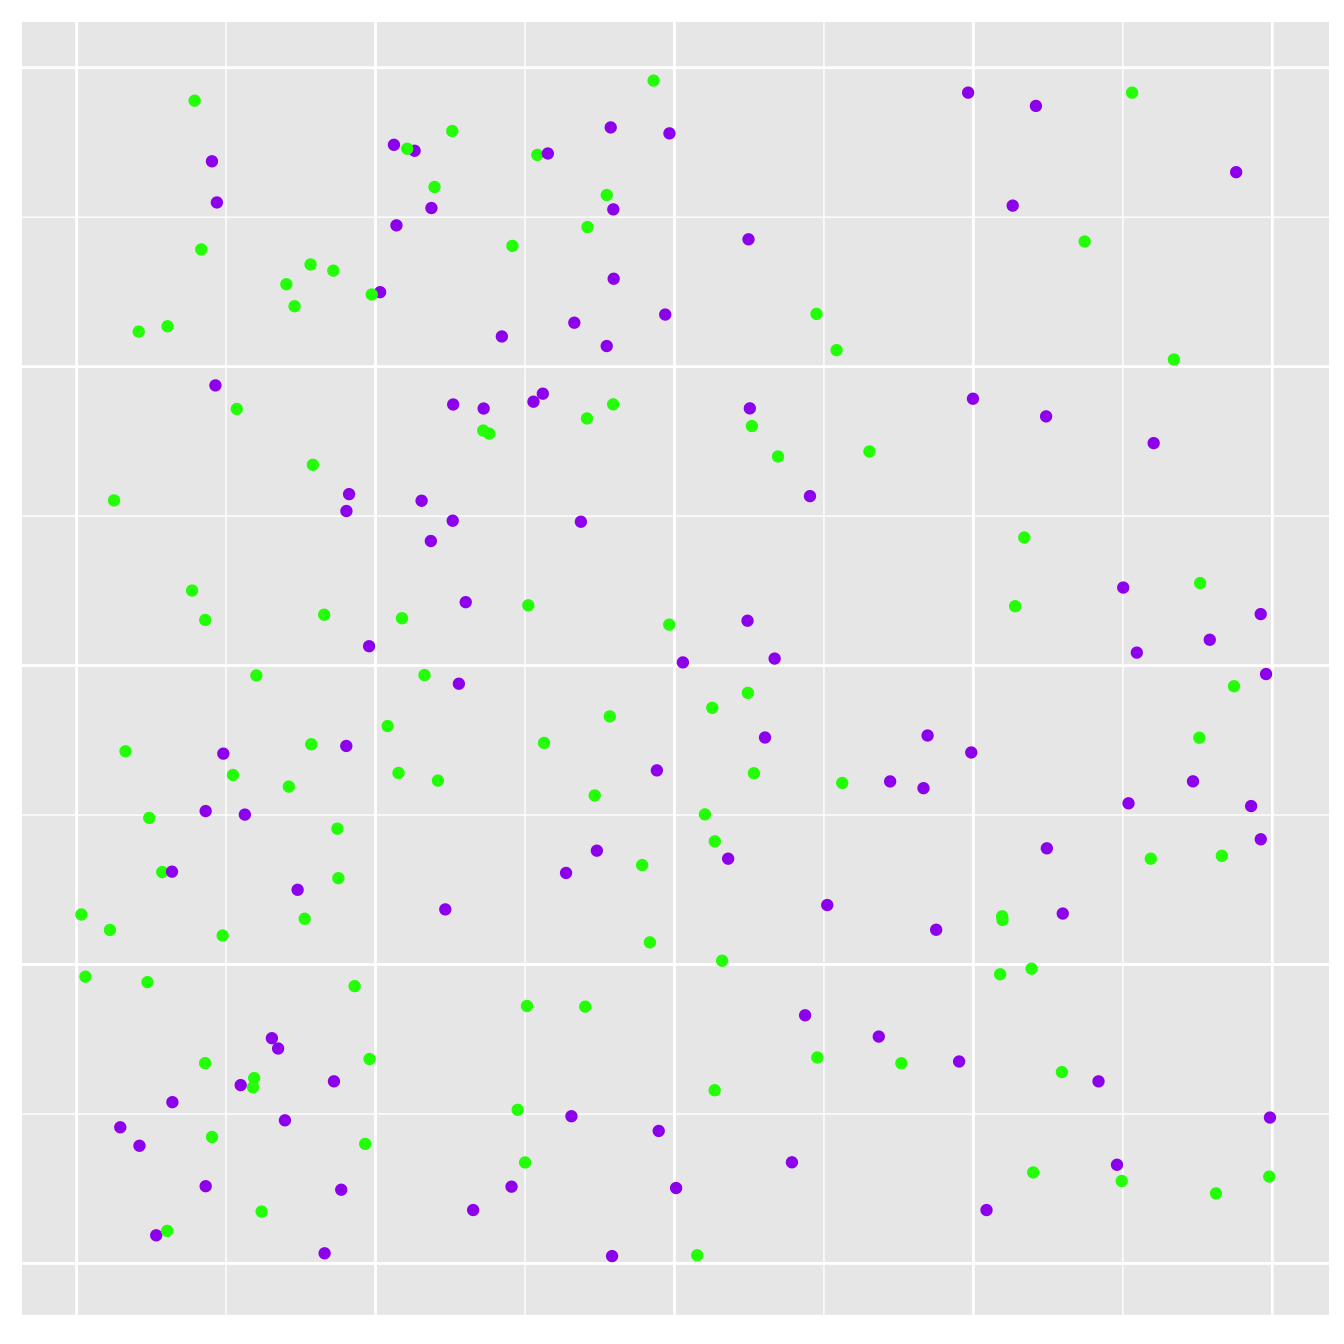
\includegraphics[width=0.5\linewidth]{intro-bio-stats-book_files/figure-latex/plants-all-1} 

}

\caption{Stylised landscape showing a population of purple and green plants}\label{fig:plants-all}
\end{figure}

These are idealised data generated using a simulation in R but proceed as though these they real.

\hypertarget{step-1-refine-your-questions-hypotheses-and-predictions-1}{%
\subsubsection*{Step 1: Refine your questions, hypotheses and predictions}\label{step-1-refine-your-questions-hypotheses-and-predictions-1}}
\addcontentsline{toc}{subsubsection}{Step 1: Refine your questions, hypotheses and predictions}

Imagine we had also previously studied a different population of this species that exhibits the same polymorphism. We think the two populations were once connected but habitat loss has isolated them. Our previous studies with the old neighbouring population have shown:

\begin{itemize}
\item
  A single gene with two alleles controls the colour polymorphism: a recessive mutant allele (`P') confers the purple colour and the dominant wild-type allele (`G') makes plants green. Genetic work has shown that the two alleles are present in a ratio of about 1:1 in the neighbouring population.
\item
  There seems to be no observable fitness difference between the two morphs in the neighbouring population. What's more, about 25\% of plants are purple. This suggests that the two alleles are in \href{https://en.wikipedia.org/wiki/Hardy–Weinberg_principle}{Hardy-Weinberg equilibrium}. These two observations suggest that there is no selection operating on the polymorphism.
\end{itemize}

Things are different in the new study population. The purple morph seems to be about as common as the green morph, and preliminary research indicates purple plants seem to produce more seeds than green plants. Our \textbf{hypothesis} is, therefore, that purple plants have a fitness advantage in the new study population. Our \textbf{prediction} is that the frequency of the purple morph will be greater than 25\% in the new study population, as selection is driving the `P' allele to fixation.

(This isn't the strongest test of our hypothesis, by the way. Really, we need to study allele and genotype frequencies, not just phenotypes. It is good enough for illustrative purposes.)

\hypertarget{step-2-decide-which-population-is-important}{%
\subsubsection*{Step 2: Decide which population is important}\label{step-2-decide-which-population-is-important}}
\addcontentsline{toc}{subsubsection}{Step 2: Decide which population is important}

This situation is made up, so consideration of the statistical population is a little artificial. In the real world, we would consider various factors, such as whether or not we can study the whole population or must restrict ourselves to one sub-population. Working at a large scale should produce a more general result, but it could also present a significant logistical challenge.

\hypertarget{step-3-decide-which-variables-to-study-1}{%
\subsubsection*{Step 3: Decide which variables to study}\label{step-3-decide-which-variables-to-study-1}}
\addcontentsline{toc}{subsubsection}{Step 3: Decide which variables to study}

This step is easy. We could measure all kinds of different attributes of the plants---biomass, height, seed production, etc---but to study the polymorphism, we only need to collect information about the colour of different individuals. This means we are going to be working with a nominal variable that takes two values: `purple' or `green'.

\hypertarget{step-4-decide-which-population-parameters-are-relevant-1}{%
\subsubsection*{Step 4: Decide which population parameters are relevant}\label{step-4-decide-which-population-parameters-are-relevant-1}}
\addcontentsline{toc}{subsubsection}{Step 4: Decide which population parameters are relevant}

The prediction we want to test is about the purple morph frequency, or equivalently, the percentage, or proportion, of purple plants. Therefore, the relevant population parameter is the frequency of purple morphs in the wider population. We need to collect data that would allow us learn about this unknown quantity.

\hypertarget{step-5-gather-a-representative-sample-1}{%
\subsubsection*{Step 5: Gather a representative sample}\label{step-5-gather-a-representative-sample-1}}
\addcontentsline{toc}{subsubsection}{Step 5: Gather a representative sample}

A representative sample in this situation is one in which every individual on the landscape has the same probability of being sampled. This is what people mean when they refer to a `random sample'. Gathering a random sample of organisms from across a landscape is surprisingly hard to do. Fortunately, it is very easy to do in a simulation. Let's seen what happens if we sample 20 plants at random\ldots{}

\begin{figure}

{\centering 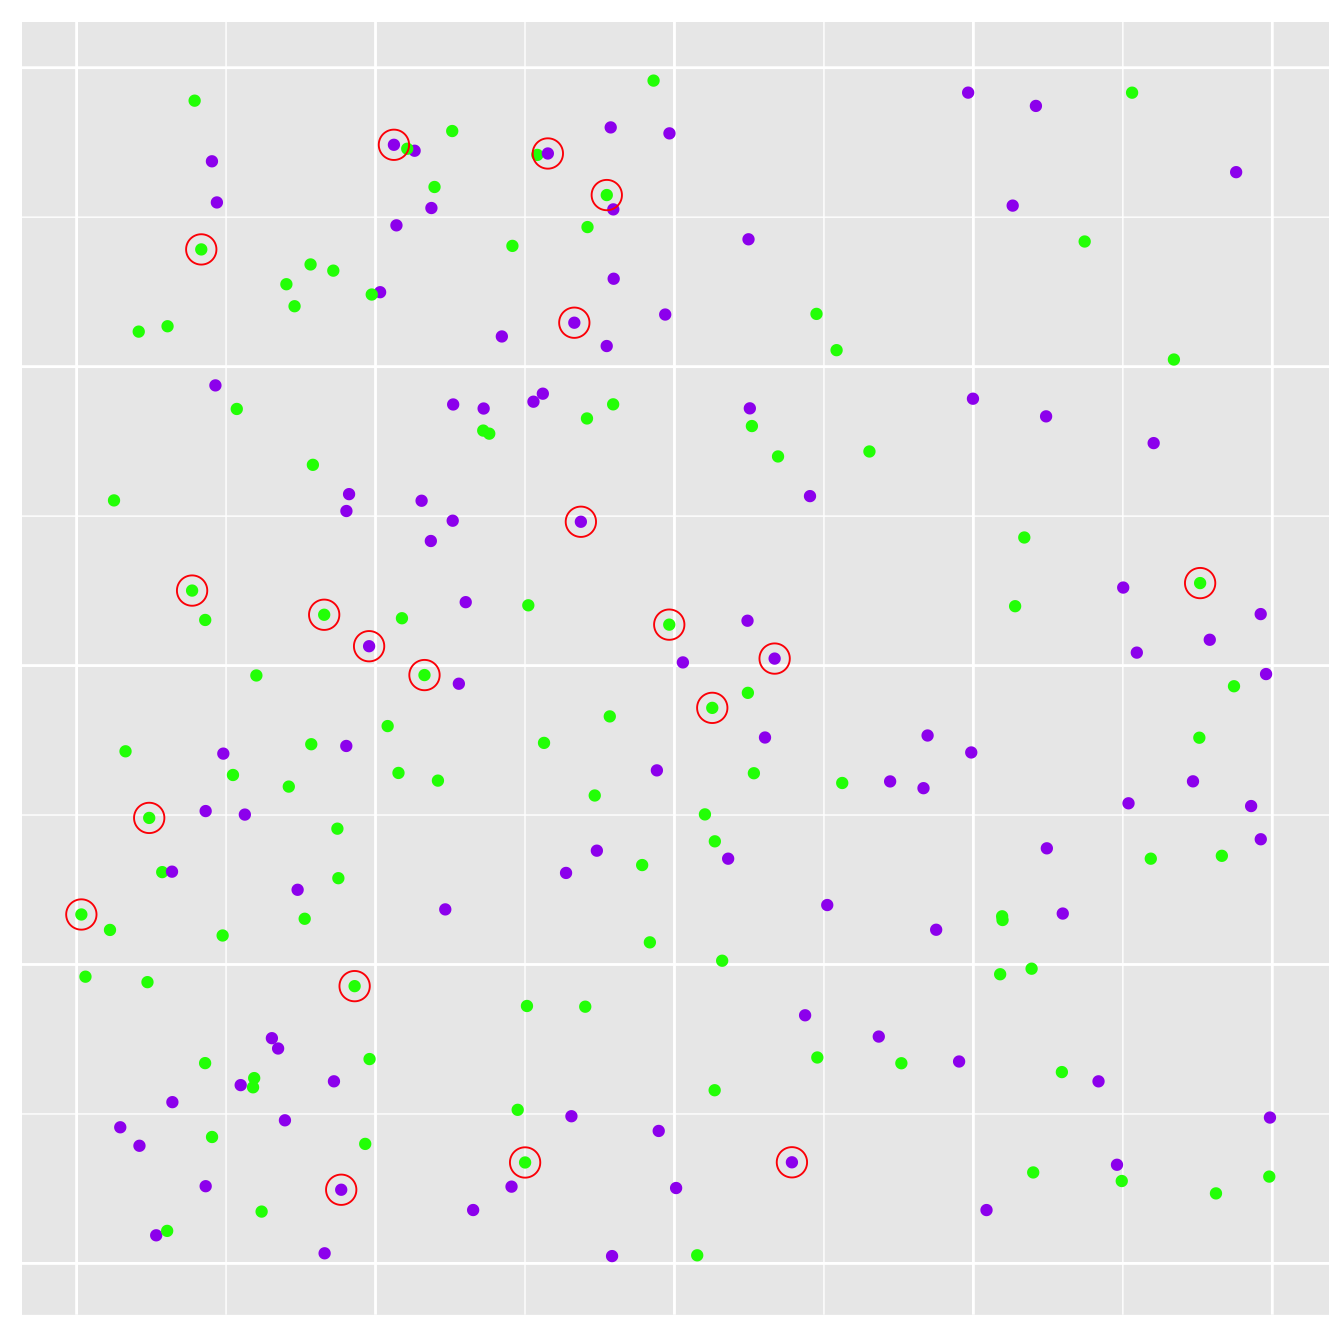
\includegraphics[width=0.5\linewidth]{intro-bio-stats-book_files/figure-latex/plants-samp1-1} 

}

\caption{Sampling plants. Sampled plants are circled in red}\label{fig:plants-samp1}
\end{figure}

The new plot shows the original population of plants, only this time we've circled the sampled individuals in red. We would only `see' this sample of plants in the real world.

\hypertarget{step-6-estimate-the-population-parameter-1}{%
\subsubsection*{Step 6: Estimate the population parameter}\label{step-6-estimate-the-population-parameter-1}}
\addcontentsline{toc}{subsubsection}{Step 6: Estimate the population parameter}

Estimating a frequency from a sample is simple enough though we can express frequencies in different ways. We'll use a percentage. We found 12 green plants and 8 purple plants in our sample, which means our point estimate of the purple morph frequency is 40\%. This is certainly greater than 25\%---the value observed in the original population---but it isn't that far off when you consider this is from a small sample.

\hypertarget{now-what}{%
\section{Now what?}\label{now-what}}

Maybe the purple plants aren't at a selective advantage after all? Or perhaps they are? We'll need to develop a rigorous statistical test of some kind to evaluate our prediction. Before we can do this we need to delve into a few more concepts. The first, sampling error, is needed describe the uncertainty in the purple morph frequency estimate (step 7). We'll look at this topic in the next chapter. After that, we'll be in the position to answer our question about differences among the two populations (step 8).

\hypertarget{part-statistical-concepts}{%
\part{Statistical Concepts}\label{part-statistical-concepts}}

\hypertarget{sampling-error}{%
\chapter{Sampling error}\label{sampling-error}}

In the previous chapter, we introduced the idea that point estimates of a population parameter are always imperfect in that they won't exactly match its true value. This uncertainty is unavoidable. This means it is not enough to have estimated something to `do statistics'---we have to also know about uncertainty of the estimate. We use the machinery of statistics to quantify this uncertainty. Once we have pinned down the uncertainty, we can start to provide meaningful answers to our scientific questions.

We will arrive at the `getting to the answer step' in the next chapter. First, we have to develop the uncertainty idea by considering sampling error, sampling distributions and standard errors.

\hypertarget{sampling-error-1}{%
\section{Sampling error}\label{sampling-error-1}}

For now, let's continue with the plant polymorphism example from the previous chapter. We had taken one sample of 20 plants from our hypothetical population and found that the frequency of purple plants in that sample was 40\%. This is a point estimate of purple plant frequency based on a random sample of 20 plants.

What happens if we repeat that same sampling process to arrive at a new, completely independent sample? This is what the population looks like, along with this new sample highlighted with red circles:

\begin{figure}

{\centering 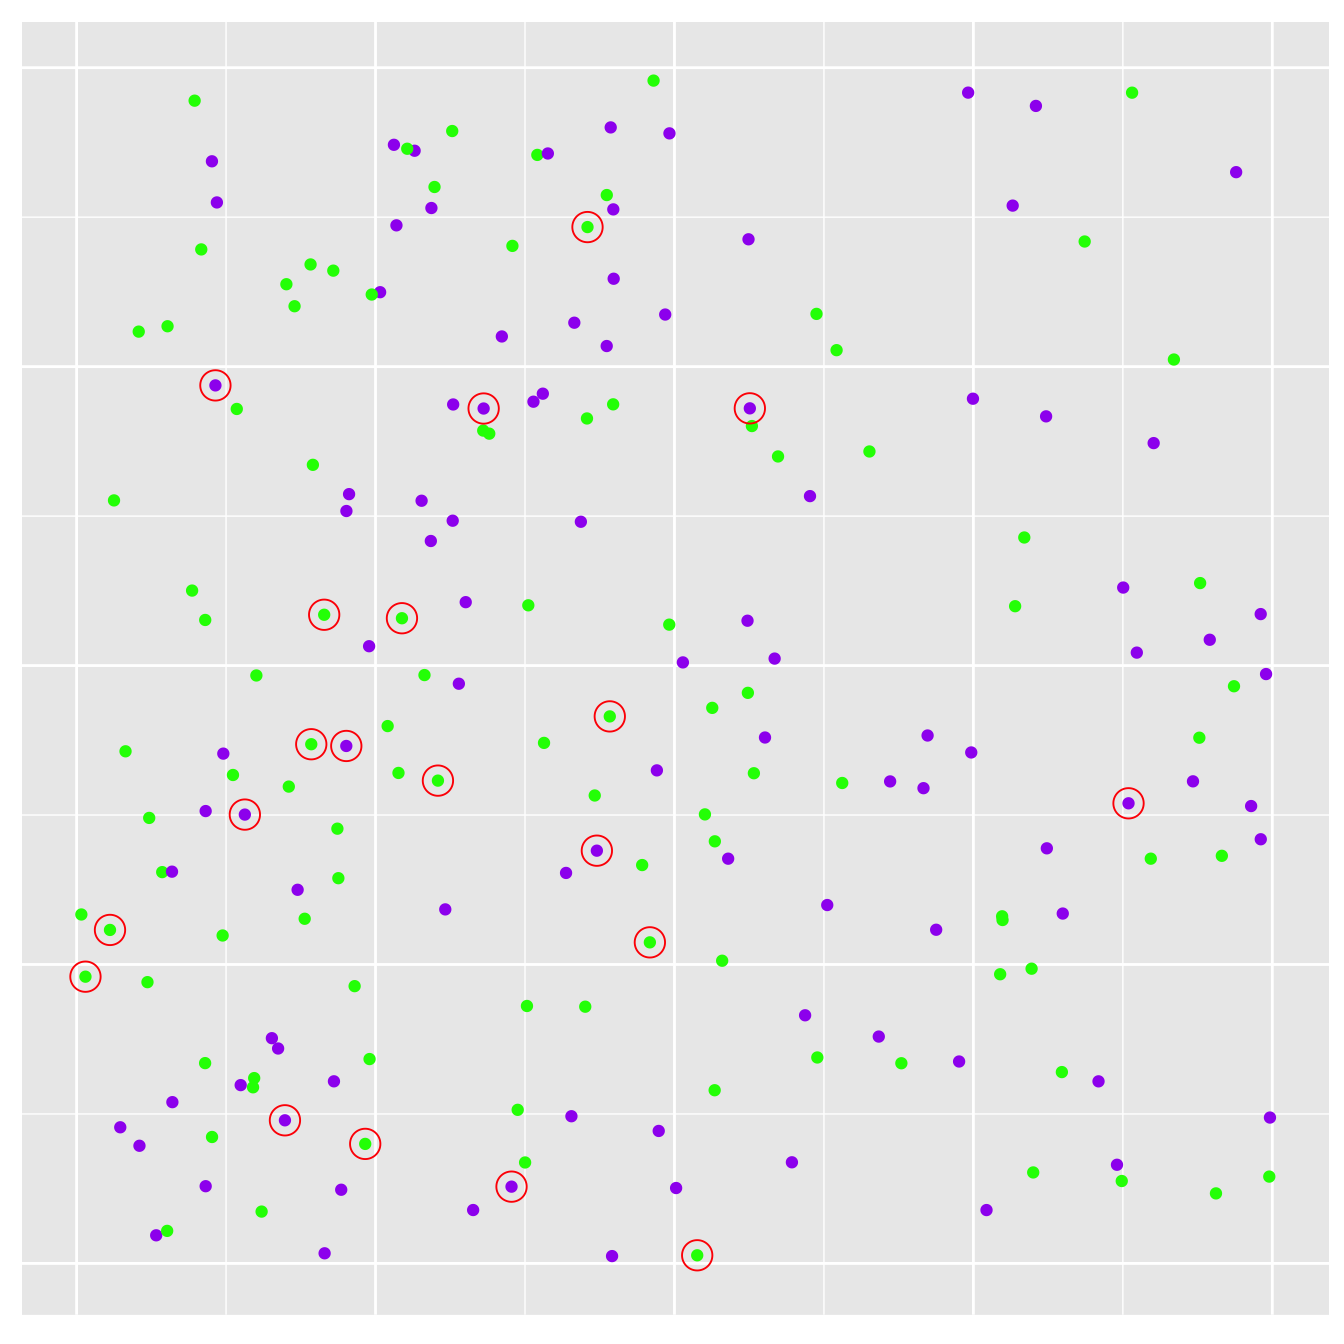
\includegraphics[width=0.5\linewidth]{intro-bio-stats-book_files/figure-latex/plants-samp2-1} 

}

\caption{Plants sampled on the second occasion}\label{fig:plants-samp2}
\end{figure}

This time we ended up sampling 11 green plants and 9 purple plants, so our second estimate of the purple morph frequency is 45\%. This estimate is quite different from the first one. It is lower than that seen in the original study population. Our hypothesis that the purple morph is more prevalent in the new population is beginning to look a little shaky now.

Nothing about the study population changed between the first and second samples. What's more, we used a completely reliable sampling scheme to generate these samples---there was nothing biased or incorrect about the way individuals were sampled. The two different estimates of purple morph frequency arise from nothing more than chance variation in the sampling process.

This variation--present whenever we observe a sample---has a special name. It is called \textbf{sampling error}. The word `error' has nothing to do with mistakes or problems. In statistics, it used to refer to the variability or `noise' in some process. Sampling error is the reason why we have to use statistics. Every time we estimate something, there's some sampling error lurking in the estimate. If we ignore it, we risk drawing incorrect conclusions about the world.

(By the way, another name for sampling error is `sampling variation'. We'll use both terms in this book because they are both widely used)

It is important to realise that sampling error is not really a property of any particular sample. It is a consequence of the nature of the variable(s) we're studying and the sampling method used to investigate the population. We can start to understand what all this means by considering something called a sampling distribution.

\hypertarget{sampling-distributions}{%
\section{Sampling distributions}\label{sampling-distributions}}

We can use our simple simulation to explore sampling error. This time, rather than taking one sample at a time, we will simulate thousands of independent samples. The number of plants sampled (`n') will always be 20. Every sample will be drawn from the same population, i.e.~the population parameter (purple morph frequency) will never change across samples. This means any variation we observe is due to nothing more than sampling error.

Here is a graphical summary of one such repeated simulation exercise:

\begin{figure}

{\centering 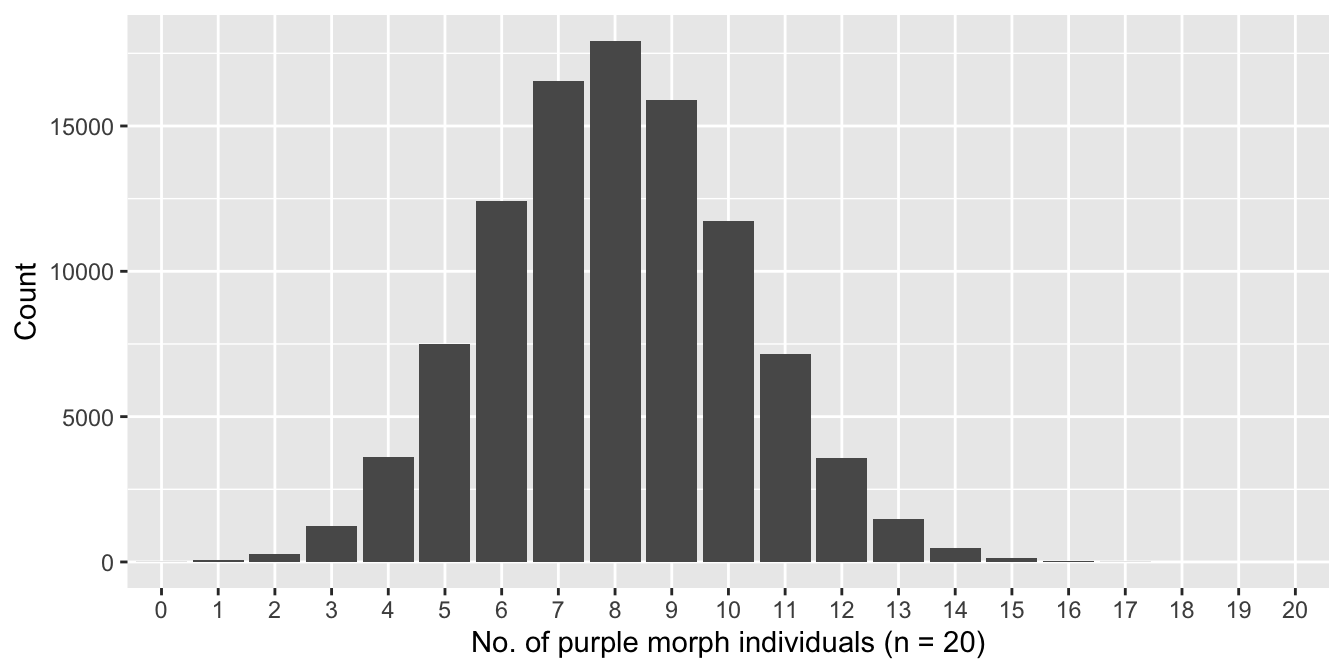
\includegraphics[width=1\linewidth]{intro-bio-stats-book_files/figure-latex/samp-dist-1-1} 

}

\caption{Distribution of number of purple morphs sampled (n = 20)}\label{fig:samp-dist-1}
\end{figure}

This bar plot summarises the results from taking 100000 independent samples of our population. We took 20 individuals from our hypothetical population and calculated the number of purple morphs seen each time. The bar plot shows the number of times we found 0, 1, 2, 3, \ldots{} purple individuals, all the way up to the maximum possible (20). Notice that we're summarising the distribution of purple morph counts rather than percentages at this point (either is fine).

This distribution has a special name. It is called a \textbf{sampling distribution}. To work this out, we have to postulate values for the population parameters, and we have to know how the population was sampled. This can often be done using mathematical reasoning. However, we used a brute-force simulation to approximate the sampling distribution of purple morph counts that arises when we sample 20 individuals from the hypothetical population.

What does this particular sampling distribution show? It summarises the range of outcomes we can expect to observe when we repeat the same sampling process over and over again. The most common outcome is eight purple morphs, which would yield an estimate of 8/20 = 40\% for the purple morph frequency.

Although there is no way to know this without being told, a 40\% purple morph frequency is the number used to simulate the original hypothetical data set. It turns out that in this instance, the true value of the parameter we're trying to learn about also happens to be the most common estimate we expect to see under repeated sampling.

Returning to our question---what is the purple morph frequency---we now have our answer. The purple morph frequency is 40\%. Ok, but we obviously `cheated' here because we used information from 1000s of samples to arrive at that answer. In the real world we typically have to work with only one sample. We'll see out how to use that one sample to learn the purple morph frequency later.

What use is the sampling distribution idea? It turns out that sampling distributions are key to `doing frequentist statistics'. To understand why we need to look a bit more carefully at that sampling distribution we made. Look at its spread along the x-axis. The range of outcomes is roughly 2 to 15, corresponding to estimated purple morph frequencies of 10-75\%. This shows that when we sample 20 individuals, the sampling error for a frequency estimate can be quite large.

The sampling distribution we summarised above is only relevant for the case where 20 individuals are sampled and the frequency of purple plants in the population is 40\%. If we change either of those two numbers and rerun the repeated sampling process we will end up with a different sampling distribution. That's what was meant by, ``It \textless sampling error\textgreater{} is a consequence of the nature of the variable(s) we're studying and the sampling method used to investigate the population.''

Once we know how to construct the sampling distribution for a particular problem, we can start making statements about sampling error to quantify uncertainty, and eventually, answer scientific questions. Fortunately, we don't have to work any of the details out for ourselves---a lot of clever statisticians have already done the hard work for us!

\hypertarget{the-effect-of-sample-size}{%
\section{The effect of sample size}\label{the-effect-of-sample-size}}

One of the most important aspects of a sampling scheme is the \textbf{sample size} ---often denoted `n'. This is the number of observations of objects, items, etc, in a sample. To get a sense of why sample size matters, we'll repeat in our sampling exercise using two new sample sizes. First we'll use a sample size of 40 individuals, then we'll take a sample of 80 individuals. As before, we'll take a total of 100000 repeated samples from the population.

Here's a graphical summary of the resulting sampling distributions:

\begin{figure}

{\centering 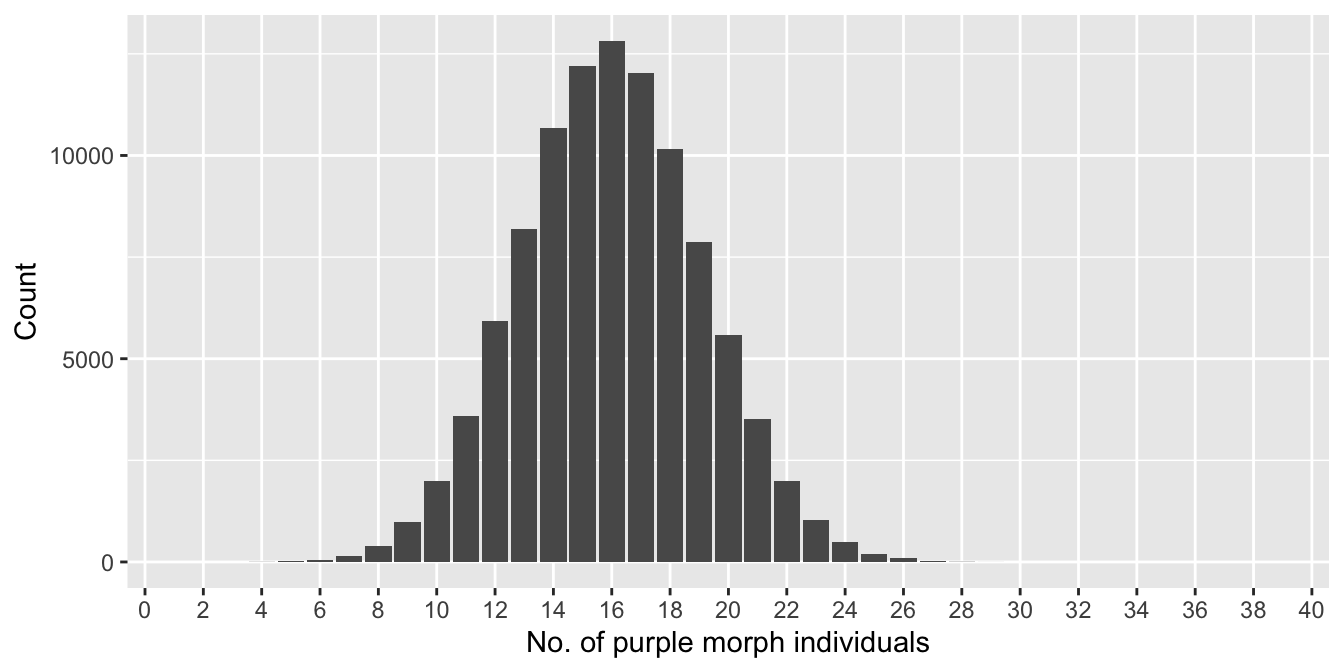
\includegraphics[width=1\linewidth]{intro-bio-stats-book_files/figure-latex/samp-dist-2-1} 

}

\caption{Distribution of number of purple morphs sampled (n = 40)}\label{fig:samp-dist-2}
\end{figure}

\begin{figure}

{\centering 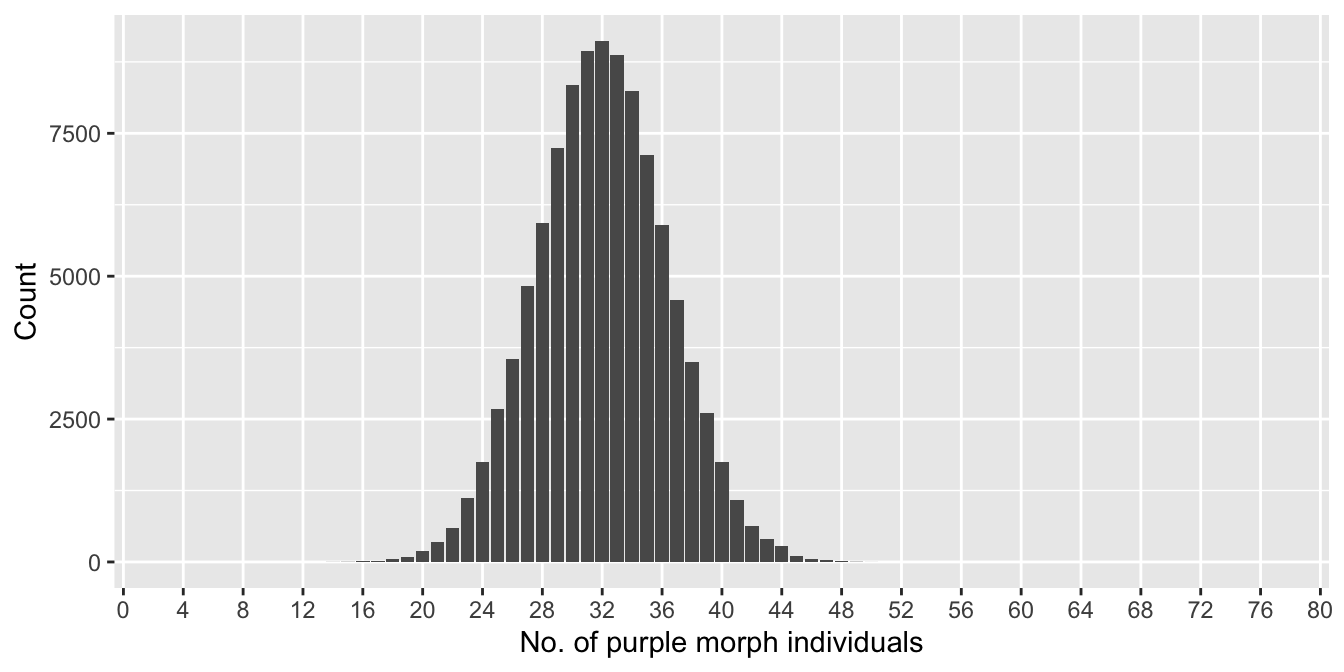
\includegraphics[width=1\linewidth]{intro-bio-stats-book_files/figure-latex/samp-dist-3-1} 

}

\caption{Distribution of number of purple morphs sampled (n = 80)}\label{fig:samp-dist-3}
\end{figure}

We plotted each of them over the full range of possible outcomes, i.e.~the x axis runs from 0-40 and 0-80, respectively, in both plots. This is important because it allows us to compare the spread of each sampling distribution relative to the range of all possible outcomes. What do these two plots tell us about the effect of changing sample size?

The range of outcomes in the first plot (n = 40) is roughly 6 to 26, corresponding to estimated purple morph frequencies in the range of 15-65\%. The range of outcomes in the second plot (n = 80) is roughly 16 to 48, corresponding to estimated frequencies in the range of 20-60\%. The implications of this basic assessment are clear: we reduced sampling error by increasing the sample size. This makes intuitive sense. The composition of a large sample should more closely approximate that of the true population than a small sample.

How much data do we need to collect to accurately estimate a frequency? Here is the approximate sampling distribution of the purple morph frequency estimate when we sample 500 individuals:

\begin{verbatim}
## Warning: Removed 2 rows containing missing values (geom_bar).
\end{verbatim}

\begin{figure}

{\centering 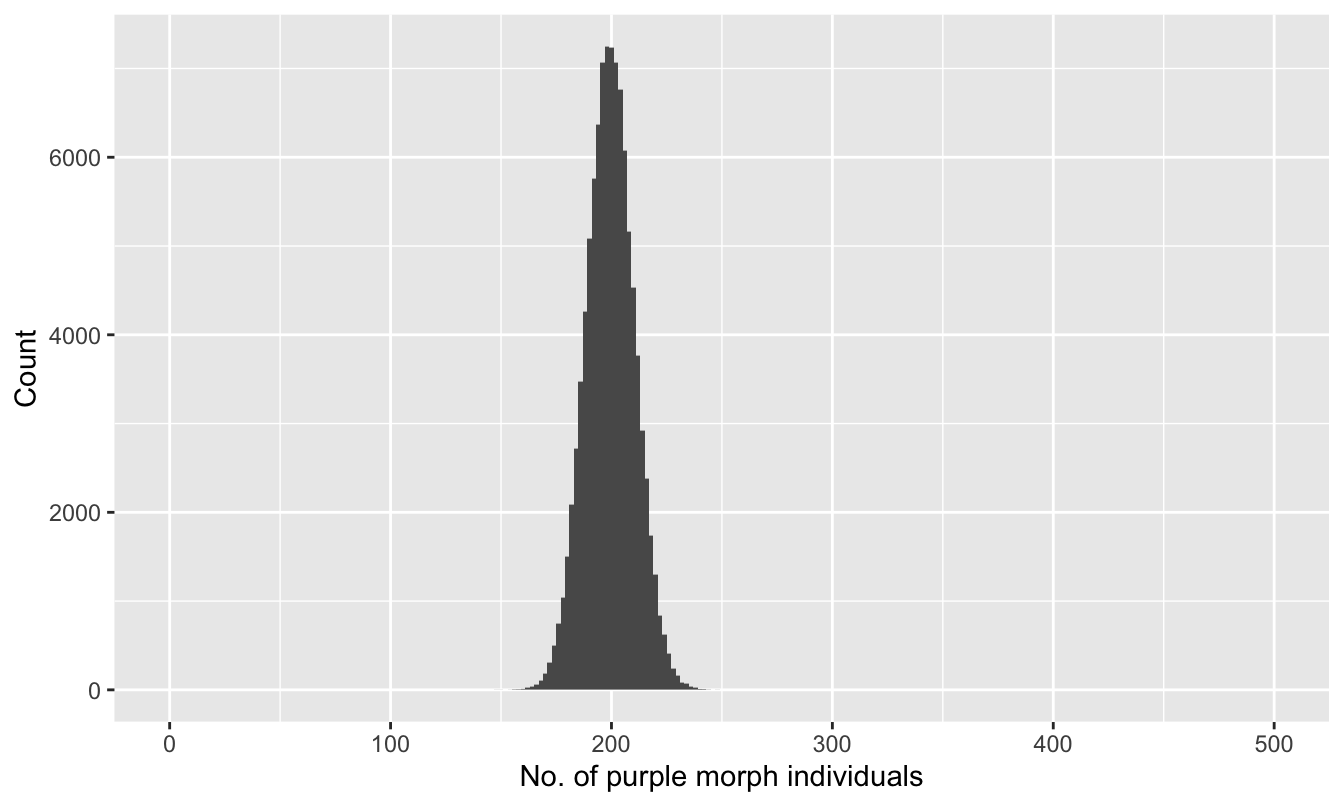
\includegraphics[width=1\linewidth]{intro-bio-stats-book_files/figure-latex/samp-dist-big-1} 

}

\caption{Distribution of number of purple morphs sampled (n = 500)}\label{fig:samp-dist-big}
\end{figure}

This time the range of outcomes is about 160 to 240, corresponding to purple morph frequencies in the 32-48\% range. This is a big improvement over the smaller samples we just considered, but still, even with 500 individuals in a sample, we still expect quite a lot of uncertainty in our estimate. The take-home message is that we need a lot of data to reduce sampling error.

\hypertarget{the-standard-error}{%
\section{The standard error}\label{the-standard-error}}

We've not been very careful about how we quantify the spread of a sampling distribution so far---we just estimated the range of purple morph counts by looking at histograms. This is fine for an investigation of general patterns, but to make rigorous comparisons, we need a quantitative measure of sampling error variation. One such quantity is called the \textbf{standard error}.

The standard error is quite a simple idea, though its definition is a bit of mouthful: the standard error of an estimate is the standard deviation of the estimate's sampling distribution. Don't worry if that is confusing! Everyone finds the definition of standard error confusing when they first encounter it. The key point is that it is a measure of the spread, or dispersion, of a distribution. That distribution is the sampling distribution associated with some kind of estimate.

(It is common to use a shorthand abbreviations such ``SE'', ``S.E.'', ``se'' or ``s.e.'' in place of `standard error' when referring to the standard error in text.)

It's much easier to make sense of something abstract, like a standard error, by looking at a concrete example. Let's calculate the standard error of the estimated purple morph frequency. It is possible to do this using mathematical reasoning; however, it is much easier to understand what's happening if we use `brute force' simulations in R.

We'll show you the code to do this but there's no need to commit any of it to memory. It's included for readers who like to see how things work. We start by specifying the number of samples to take (\texttt{n\_samples}), the sample size to use for each sample (\texttt{sample\_size}), and the value of the population morph frequency (\texttt{purple\_prob}). We set up the simulation by creating these variables:

\begin{Shaded}
\begin{Highlighting}[]
\CommentTok{\# number of independent samples}
\NormalTok{n\_samples }\OtherTok{\textless{}{-}} \DecValTok{100000}
\CommentTok{\# sample size to use for each sample}
\NormalTok{sample\_size }\OtherTok{\textless{}{-}} \DecValTok{80}
\CommentTok{\# probability a plant will be purple}
\NormalTok{purple\_prob }\OtherTok{\textless{}{-}} \FloatTok{0.4}
\end{Highlighting}
\end{Shaded}

This sets up a simulation to calculate the expected standard error when the purple morph frequency is 40\% and the sample size is 80, using \ensuremath{10^{5}} samples. The next step requires a bit more knowledge of R and probability theory:

\begin{Shaded}
\begin{Highlighting}[]
\CommentTok{\# repeat the sampling/estimation procedure many times}
\NormalTok{raw\_samples }\OtherTok{\textless{}{-}} \FunctionTok{rbinom}\NormalTok{(}\AttributeTok{n =}\NormalTok{ n\_samples, }\AttributeTok{size =}\NormalTok{ sample\_size, }\AttributeTok{prob =}\NormalTok{ purple\_prob)}
\CommentTok{\# convert results to \%}
\NormalTok{percent\_samples }\OtherTok{\textless{}{-}} \DecValTok{100} \SpecialCharTok{*}\NormalTok{ raw\_samples }\SpecialCharTok{/}\NormalTok{ sample\_size}
\end{Highlighting}
\end{Shaded}

The details of the R code are not important here. A minimum of A-level statistics is needed to understand what the \texttt{rbinom} function is doing, but in a nutshell, it is the workhorse that runs the simulation. Mostly, we're showing the code to demonstrate that seemingly complex things are often easy to do in R.

What matters here is the result. This is stored the result in a vector called \texttt{percent\_samples}. Here are its first 50 values:

\begin{verbatim}
##  [1] 33.75 35.00 42.50 41.25 46.25 35.00 42.50 45.00 43.75 40.00 41.25 52.50
## [13] 43.75 38.75 38.75 47.50 42.50 40.00 43.75 42.50 36.25 42.50 43.75 43.75
## [25] 35.00 42.50 35.00 37.50 41.25 40.00 45.00 40.00 41.25 38.75 46.25 45.00
## [37] 31.25 40.00 47.50 42.50 37.50 41.25 31.25 45.00 32.50 36.25 40.00 37.50
## [49] 40.00 45.00
\end{verbatim}

These numbers are all part of the sampling distribution of morph frequency estimates. Each value is one possible estimate of the purple morph frequency when we sample 80 individuals from a population where the true value is 40\%. There are \ensuremath{10^{5}} such estimates stored in \texttt{percent\_samples}.

How do we then calculate the standard error? This is \emph{defined} as the standard deviation of the sampling distribution that we just constructed with a simulation. So all we need to do now is calculate their standard deviation using the \texttt{sd} function:

\begin{Shaded}
\begin{Highlighting}[]
\FunctionTok{sd}\NormalTok{(percent\_samples)}
\end{Highlighting}
\end{Shaded}

\begin{verbatim}
## [1] 5.494663
\end{verbatim}

The standard error is about 5.5. Why is this number useful? It gives us a means to reason about the variability in a sampling distribution. When a sampling distribution is `well-behaved', then roughly speaking, about 95\% of estimates are expected to lie within a range of about four standard errors.

Not convinced? Look at the second bar plot we produced, where the sample size was 80 and the purple morph frequency was 40\%. What is the approximate range of simulated values? How close is this to \(4 \times 5.5\)? Quite close!

In summary, the standard error quantifies the variability of a sampling distribution. We said in the previous chapter that a point estimate is largely useless without an associated measure of uncertainty. The standard error is one such measure.

\hypertarget{what-is-the-point-of-all-this}{%
\section{What is the point of all this?}\label{what-is-the-point-of-all-this}}

Why have we just spent so much time looking at what happens when we take repeated samples from a population with known properties? When we collect data in the real world, we only have the luxury of working with a small number of samples---usually just one, in fact. We also won't know anything much about the population parameter of interest in that situation. This lack of knowledge is the reason for collecting data in the first place!

The short answer is that before we can use frequentist statistics, we need to have a sense of:

\begin{itemize}
\tightlist
\item
  how point estimates behave under repeated sampling (i.e.~\textbf{sampling distributions}),
\item
  and how \textbf{sampling error} and \textbf{standard error} relate to sampling distributions.
\end{itemize}

Once we understand those ideas, we can start to make sense of how frequentist statistical tests work. That's what we'll do in the next few chapters.

\hypertarget{statistical-significance-and-p-values}{%
\chapter{\texorpdfstring{Statistical significance and \emph{p}-values}{Statistical significance and p-values}}\label{statistical-significance-and-p-values}}

Frequentist statistics works by answering the following question: \emph{what would have happened}~if we repeated a data collection exercise many times, \emph{assuming that the population remains the same}~each time. This is the idea we used to generate sampling distributions in the previous chapter. The details of this procedure depend on what kind of question we are asking.

What is common to every frequentist technique is that we ultimately have to work out what some sort of sampling distribution looks like. Once we've done that, we can evaluate how likely a particular result is. This naturally leads to the most important ideas in frequentist statistics: \emph{p}-values and statistical significance.

\hypertarget{bootstrap}{%
\section{Estimating a sampling distribution}\label{bootstrap}}

Let's carry on with the plant polymorphism example. Our ultimate goal is to determine if the purple morph frequency is likely to be greater than 25\% in the new study population. The suggestion above is that we will need to determine the sampling distribution of purple morph frequency estimates to get to this point.

At first glance, this seems like an impossible task because we only have access to a single sample. The solution to this problem is surprisingly simple: use the one sample to approximate the population somehow, then work out what the sampling distribution of our estimate should look like by `taking samples' from this approximation.

We'll unpack this idea a bit more before we try it out for real.

\hypertarget{bootstrap-overview}{%
\subsection{Overview of bootstrapping}\label{bootstrap-overview}}

There are many ways to use a sample to approximate the population. One of the simplest is to \emph{pretend the sample is the true population}. We can then draw new samples from this pretend population to get at a sampling distribution. This may sound like `cheating', but it turns out this is a perfectly valid way to construct approximate sampling distributions.

We'll try to understand how this works by using a physical analogy based on our plant morph example. Imagine that we have written down the colour of every sampled plant on a different piece of paper and then placed these bits of paper into a hat. We then do the following:

\begin{enumerate}
\def\labelenumi{\arabic{enumi}.}
\tightlist
\item
  Pick a piece of paper at random, record its value (purple or green), put the paper back into the hat, and shake the hat about to mix up the bits of paper.
\end{enumerate}

(The shaking here is meant to ensure that each piece of paper has an equal chance of being picked.)

\begin{enumerate}
\def\labelenumi{\arabic{enumi}.}
\setcounter{enumi}{1}
\item
  Now pick another piece of paper (we might get the same one), record its value, put that one back into the hat, and shake everything up again.
\item
  Repeat this process until we have a recorded new sample of colours that is the same size as the real sample. We have now have generated a `new sample' from the original one.
\end{enumerate}

(This process is called `sampling with replacement'. Each artificial sample is called a `bootstrapped sample'.)

\begin{enumerate}
\def\labelenumi{\arabic{enumi}.}
\setcounter{enumi}{3}
\item
  For each bootstrapped sample, calculate whatever quantity is of interest. In our example, this is the proportion of purple plants sampled.
\item
  Repeat steps 1-4 until we have generated a large number of bootstrapped samples. About 10000 is sufficient for most problems.
\end{enumerate}

Although it seems like cheating, this procedure really does approximate the sampling distribution of the purple plant frequency. It is called \textbf{bootstrapping} (or `the bootstrap').

The bootstrap is quite a sophisticated technique developed by statistician \href{https://en.wikipedia.org/wiki/Bradley_Efron}{Bradley Efron}. We're not going to use it to solve real data analysis problems and there's no need to learn how to do it. We're introducing bootstrapping because it provides an intuitive way to understand how frequentist methodology works without getting stuck into any challenging mathematics.

\hypertarget{doing-it-for-real}{%
\subsection{Doing it for real}\label{doing-it-for-real}}

No one carries out bootstrapping using bits of paper and hat. Generating 10000 bootstrapped samples via such a method would obviously take a very long time! Luckily, computers are very good at carrying out repetitive tasks quickly. We're going to work through how to implement the bootstrap for our hypothetical example.

\begin{infobox}{action}

\hypertarget{section}{%
\subsubsection*{}\label{section}}
\addcontentsline{toc}{subsubsection}{}

The best way to understand what follows is by actually running the example code line by line. You are encouraged to do this, but it is certainly not essential. You can gain an adequate understanding bootstrapping by simply reading through the example.

\end{infobox}

\hypertarget{set-up-and-read-the-data}{%
\subsubsection*{Set up and read the data}\label{set-up-and-read-the-data}}
\addcontentsline{toc}{subsubsection}{Set up and read the data}

Assume we had sampled 250 individuals from the new plant population. A data set representing this situation is stored in the Comma Separated Value (CSV) file called `MORPH\_DATA.CSV'. Let's assume these data have been read into a tibble called \texttt{morph\_data}, e.g.

\begin{Shaded}
\begin{Highlighting}[]
\NormalTok{morph\_data }\OtherTok{\textless{}{-}} \FunctionTok{read\_csv}\NormalTok{(}\AttributeTok{file =} \StringTok{"MORPH\_DATA.CSV"}\NormalTok{)}
\end{Highlighting}
\end{Shaded}

The data set looks like this:

\begin{Shaded}
\begin{Highlighting}[]
\NormalTok{morph\_data}
\end{Highlighting}
\end{Shaded}

\begin{verbatim}
## # A tibble: 250 x 2
##    Colour Weight
##    <chr>   <dbl>
##  1 Green    714.
##  2 Green    693.
##  3 Green    556.
##  4 Purple   654.
##  5 Green    673.
##  6 Green    661.
##  7 Green    445.
##  8 Green    482.
##  9 Green    648.
## 10 Green    858.
## # ... with 240 more rows
\end{verbatim}

This contains 250 rows and two variables: \texttt{Colour} and \texttt{Weight}. \texttt{Colour} is a categorical variable and \texttt{Weight} is a numeric variable. The \texttt{Colour} variable contains the colour of each plant in the sample. What is that \texttt{Weight} variable all about? Actually\ldots{} we don't need this now but we will use it in the next chapter.

\hypertarget{running-the-bootstrap}{%
\subsubsection*{Running the bootstrap}\label{running-the-bootstrap}}
\addcontentsline{toc}{subsubsection}{Running the bootstrap}

Now that we understand the data, we're ready to implement bootstrapping. We are going to use a few programming tricks that beginners may not have come across before. We'll explain these as we go, but there's no need to learn them. Focus on the `why'---the logic of what we're doing---rather than the `how'.

We want to construct an approximate sampling distribution for the frequency of purple morphs. That means the variable that matters is \texttt{Colour}. Rather than work with this inside the \texttt{morph\_data} data frame, we're going to pull it out using the \texttt{\$} operator and assign it a name (\texttt{plant\_morphs}):

\begin{Shaded}
\begin{Highlighting}[]
\CommentTok{\# pull out the \textquotesingle{}Colour\textquotesingle{} variable}
\NormalTok{plant\_morphs }\OtherTok{\textless{}{-}}\NormalTok{ morph\_data}\SpecialCharTok{$}\NormalTok{Colour }
\end{Highlighting}
\end{Shaded}

Next, we'll take a quick look at the values of \texttt{plant\_morphs}:

\begin{Shaded}
\begin{Highlighting}[]
\CommentTok{\# what is the set of values \textquotesingle{}plant\_morphs\textquotesingle{} can take?}
\FunctionTok{unique}\NormalTok{(plant\_morphs)}
\end{Highlighting}
\end{Shaded}

\begin{verbatim}
## [1] "Green"  "Purple"
\end{verbatim}

\begin{Shaded}
\begin{Highlighting}[]
\CommentTok{\# show the first 100 values}
\FunctionTok{head}\NormalTok{(plant\_morphs, }\DecValTok{50}\NormalTok{) }
\end{Highlighting}
\end{Shaded}

\begin{verbatim}
##  [1] "Green"  "Green"  "Green"  "Purple" "Green"  "Green"  "Green"  "Green" 
##  [9] "Green"  "Green"  "Green"  "Green"  "Green"  "Purple" "Green"  "Green" 
## [17] "Purple" "Purple" "Green"  "Green"  "Green"  "Green"  "Green"  "Purple"
## [25] "Green"  "Green"  "Green"  "Green"  "Purple" "Purple" "Green"  "Green" 
## [33] "Green"  "Purple" "Purple" "Green"  "Green"  "Green"  "Green"  "Purple"
## [41] "Green"  "Purple" "Green"  "Green"  "Purple" "Purple" "Green"  "Green" 
## [49] "Green"  "Green"
\end{verbatim}

The last line printed out the first 50 values of \texttt{plant\_morphs}. This shows that \texttt{plant\_morphs} is a simple character vector with two categories describing the plant colour morph information.

Next, we calculate and store the sample size (\texttt{samp\_size}) and the point estimate of purple morph frequency (\texttt{mean\_point\_est}) from the sample:

\begin{Shaded}
\begin{Highlighting}[]
\CommentTok{\# get the sample size form the length of \textquotesingle{}plant\_morphs\textquotesingle{}}
\NormalTok{samp\_size }\OtherTok{\textless{}{-}} \FunctionTok{length}\NormalTok{(plant\_morphs)}
\NormalTok{samp\_size}
\end{Highlighting}
\end{Shaded}

\begin{verbatim}
## [1] 250
\end{verbatim}

\begin{Shaded}
\begin{Highlighting}[]
\CommentTok{\# estimate the frequency of purple plants as a \%}
\NormalTok{mean\_point\_est }\OtherTok{\textless{}{-}} \DecValTok{100} \SpecialCharTok{*} \FunctionTok{sum}\NormalTok{(plant\_morphs }\SpecialCharTok{==} \StringTok{"Purple"}\NormalTok{) }\SpecialCharTok{/}\NormalTok{ samp\_size}
\NormalTok{mean\_point\_est}
\end{Highlighting}
\end{Shaded}

\begin{verbatim}
## [1] 30.8
\end{verbatim}

The code in the point estimate calculation says, ``add up all the cases where \texttt{plant\_morphs} is equal to `purple', divide that total by the sample size to get the proportion of purple plants in the sample, then multiply the proprtion by 100 to turn it into a percentage.'' We find that 30.8\% of plants were purple among our sample of 250 plants.

Now we're ready to start bootstrapping. For convenience, we'll store the number of bootstrap samples we want in \texttt{n\_samp} (i.e.~10000 in this case):

\begin{Shaded}
\begin{Highlighting}[]
\CommentTok{\# number of bootstrapped samples we want}
\NormalTok{n\_samp }\OtherTok{\textless{}{-}} \DecValTok{10000}
\end{Highlighting}
\end{Shaded}

Next we need to work out how to resample the values in the \texttt{plant\_morphs} vector. The \texttt{sample} function can do this for us:

\begin{Shaded}
\begin{Highlighting}[]
\CommentTok{\# resample the plant colours}
\NormalTok{samp }\OtherTok{\textless{}{-}} \FunctionTok{sample}\NormalTok{(plant\_morphs, }\AttributeTok{replace =} \ConstantTok{TRUE}\NormalTok{)}
\CommentTok{\# show the first 50 values of the bootstrapped sample}
\FunctionTok{head}\NormalTok{(samp, }\DecValTok{50}\NormalTok{) }
\end{Highlighting}
\end{Shaded}

\begin{verbatim}
##  [1] "Green"  "Purple" "Purple" "Green"  "Green"  "Purple" "Green"  "Purple"
##  [9] "Green"  "Green"  "Green"  "Green"  "Purple" "Purple" "Green"  "Green" 
## [17] "Purple" "Purple" "Green"  "Green"  "Green"  "Green"  "Green"  "Green" 
## [25] "Green"  "Green"  "Purple" "Purple" "Purple" "Purple" "Green"  "Green" 
## [33] "Green"  "Purple" "Green"  "Green"  "Purple" "Green"  "Purple" "Green" 
## [41] "Green"  "Green"  "Purple" "Purple" "Green"  "Purple" "Green"  "Purple"
## [49] "Purple" "Purple"
\end{verbatim}

The \texttt{replace\ =\ TRUE} ensures that we sample with replacement---this is the `putting the bits of paper back into the hat' part of the process.

The new \texttt{samp} variable now contains exactly one bootstrapped sample of the 250 plants in the real sample. We only need to extract one number from this---the frequency of purple morphs:

\begin{Shaded}
\begin{Highlighting}[]
\CommentTok{\# calculate the purple morph frequency in the bootstrapped sample}
\NormalTok{first\_bs\_freq }\OtherTok{\textless{}{-}} \DecValTok{100} \SpecialCharTok{*} \FunctionTok{sum}\NormalTok{(samp }\SpecialCharTok{==} \StringTok{"Purple"}\NormalTok{) }\SpecialCharTok{/}\NormalTok{ samp\_size}
\end{Highlighting}
\end{Shaded}

That's one bootstrapped value of the purple morph frequency. Fine, but we need \(\ensuremath{10^{4}}\) values. We don't want to have to keep doing this over an over `by hand'---making \texttt{second\_bs\_freq}, \texttt{third\_bs\_freq}, and so on---because this would be very slow and boring to do.

As we said earlier, computers are very good at carrying out repetitive tasks. The \texttt{replicate} function can replicate any R code many times and return the set of results. Here is some R code that repeats what we just did \texttt{n\_samp} times, storing the resulting bootstrapped values of purple morph frequency in a numeric vector called \texttt{boot\_out}:

\begin{Shaded}
\begin{Highlighting}[]
\NormalTok{boot\_out }\OtherTok{\textless{}{-}} \FunctionTok{replicate}\NormalTok{(n\_samp, \{}
\NormalTok{  samp }\OtherTok{\textless{}{-}} \FunctionTok{sample}\NormalTok{(plant\_morphs, }\AttributeTok{replace =} \ConstantTok{TRUE}\NormalTok{)}
  \DecValTok{100} \SpecialCharTok{*} \FunctionTok{sum}\NormalTok{(samp }\SpecialCharTok{==} \StringTok{"Purple"}\NormalTok{) }\SpecialCharTok{/}\NormalTok{ samp\_size}
\NormalTok{\})}
\end{Highlighting}
\end{Shaded}

The \texttt{boot\_out} vector now contains a bootstrapped sample of frequency estimates. Here are the first 30 values rounded to 1 decimal place:

\begin{Shaded}
\begin{Highlighting}[]
\FunctionTok{head}\NormalTok{(boot\_out, }\DecValTok{30}\NormalTok{) }\SpecialCharTok{\%\textgreater{}\%} \FunctionTok{round}\NormalTok{(}\DecValTok{1}\NormalTok{)}
\end{Highlighting}
\end{Shaded}

\begin{verbatim}
##  [1] 31.6 23.6 27.6 28.4 32.0 28.0 34.0 28.0 32.8 33.2 34.0 25.2 34.0 30.0 28.8
## [16] 31.6 30.0 30.0 29.2 28.0 31.2 27.6 29.6 30.4 32.8 29.6 30.4 37.2 34.4 32.0
\end{verbatim}

(We used the pipe \texttt{\%\textgreater{}\%} to make a code a bit more readable---remember, this won't work unless the \textbf{dplyr} package is loaded.)

\hypertarget{making-sense-of-the-bootstrapped-sample}{%
\subsubsection*{Making sense of the bootstrapped sample}\label{making-sense-of-the-bootstrapped-sample}}
\addcontentsline{toc}{subsubsection}{Making sense of the bootstrapped sample}

What has all this achieved? The numbers in \texttt{boot\_out} represent the values of purple morph frequency we can expect to find if we repeated the data collection exercise many times, assuming that the purple morph frequency is equal to that of the actual sample. This is a bootstrapped sampling distribution!

We can use this bootstrapped sampling distribution in a number of ways. Let's plot it first get a sense of what it looks like. A histogram is OK here because we have a reasonably large number of possible cases:

\begin{figure}

{\centering 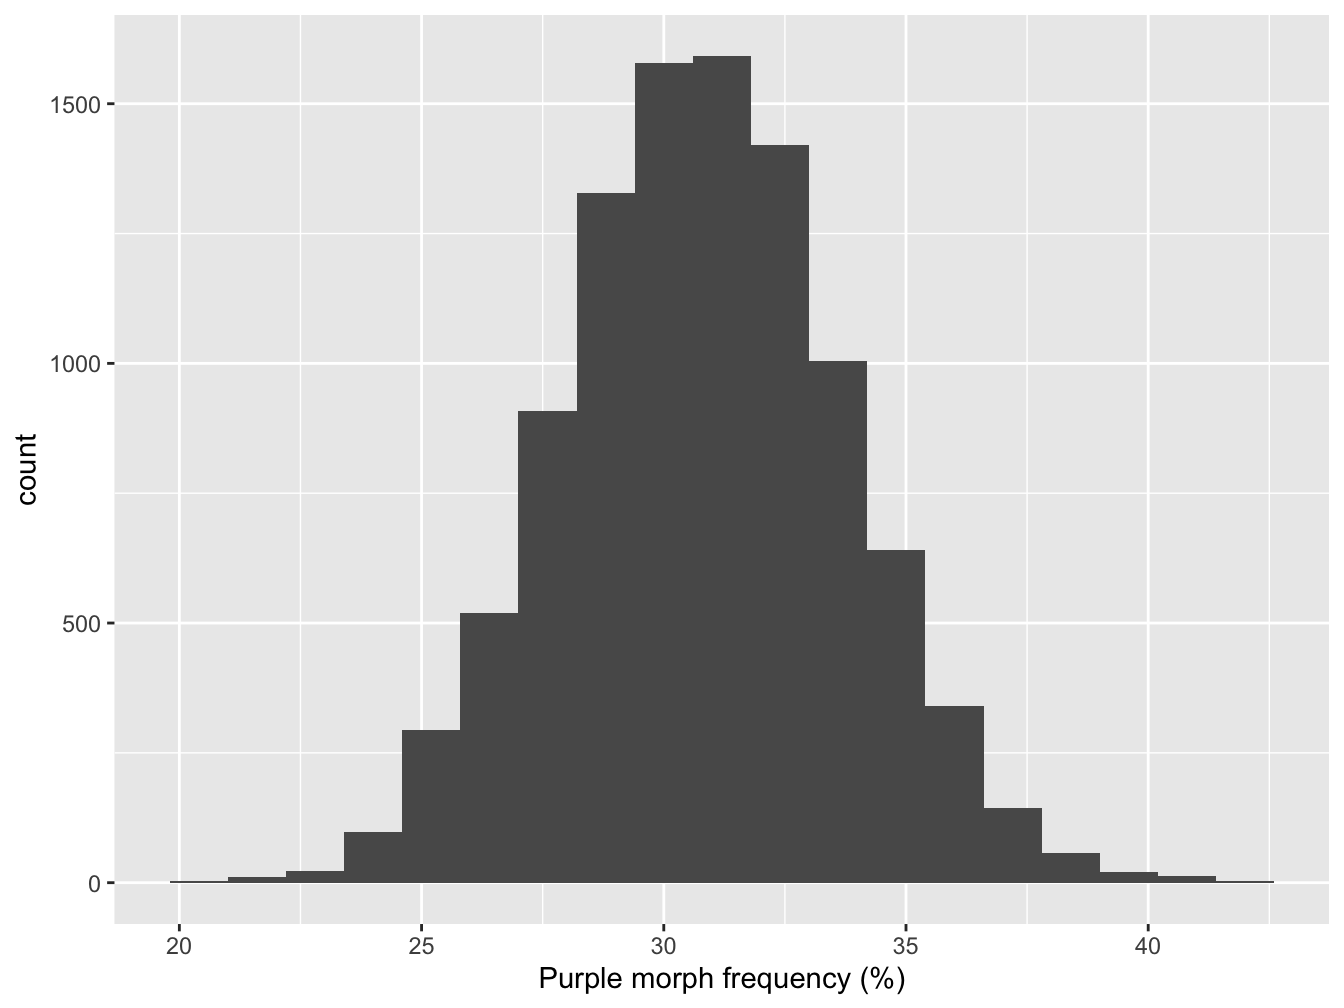
\includegraphics[width=0.75\linewidth]{intro-bio-stats-book_files/figure-latex/boot-samp-dist-1} 

}

\caption{Bootstrapped sampling distribution of purple morph frequency}\label{fig:boot-samp-dist}
\end{figure}

What the most common values in our bootstrapped sample? The centre of the distribution looks to be round about 30\%. We can be a bit more precise by calculating its mean:

\begin{Shaded}
\begin{Highlighting}[]
\FunctionTok{mean}\NormalTok{(boot\_out) }\SpecialCharTok{\%\textgreater{}\%} \FunctionTok{round}\NormalTok{(}\DecValTok{1}\NormalTok{)}
\end{Highlighting}
\end{Shaded}

\begin{verbatim}
## [1] 30.8
\end{verbatim}

This is essentially the same as the point estimate of purple morph frequency from the true sample. In fact, it is guaranteed to be the same if we construct a large enough sample because we're just resampling the data used to estimate that frequency.

A more useful quantity is the standard error (SE) of our estimate. This is \emph{defined} as being the standard deviation of the sampling distribution. We can calculate that by applying the \texttt{sd} function to the bootstrapped sample:

\begin{Shaded}
\begin{Highlighting}[]
\FunctionTok{sd}\NormalTok{(boot\_out) }\SpecialCharTok{\%\textgreater{}\%} \FunctionTok{round}\NormalTok{(}\DecValTok{1}\NormalTok{)}
\end{Highlighting}
\end{Shaded}

\begin{verbatim}
## [1] 2.9
\end{verbatim}

The standard error is a very handy quantity. Remember, it is a measure of the precision of an estimate. For example, a large SE implies that our sample size was too small to reliably estimate the population mean; a small SE means we have a reliable estimate. Once we have the point estimate of a population parameter and its standard error we're able to start asking questions like, ``is the true value likely to be different from 25\%.''

It is standard practice to include the standard error when we report a point estimate of some quantity. Whenever we report a point estimate, we really should also report its standard error, like this:

\begin{quote}
The frequency of purple morph plants (n = 250) was 30.8\% (s.e. ± 2.9).
\end{quote}

Notice we also report the sample size. More on that later in the book.

\hypertarget{statistical-significance}{%
\section{Statistical significance}\label{statistical-significance}}

Now back to the question that motivated all the work in the last few chapters. Is the purple morph frequency greater than 25\% in the new study population? The first thing to realise is that we can never answer a question like this definitively from a sample. We have to carry out some kind of probabilistic assessment instead. To make this assessment, we're going to do something that looks odd at first glance.

\begin{infobox}{warning}

\hypertarget{dont-panic}{%
\subsubsection*{Don't panic!}\label{dont-panic}}
\addcontentsline{toc}{subsubsection}{Don't panic!}

The ideas in the next section are very abstract, and you probably won't `get' them straight away. That is fine---these concepts take time to absorb and understand.

\end{infobox}

\hypertarget{carrying-out-the-assessment}{%
\subsection*{Carrying out the assessment}\label{carrying-out-the-assessment}}
\addcontentsline{toc}{subsection}{Carrying out the assessment}

We need to make two assumptions to arrive at our probabilistic assessment of whether or not the purple morph frequency is greater than 25\%:

\begin{enumerate}
\def\labelenumi{\arabic{enumi}.}
\item
  Assume the true value of the purple morph frequency in our new study population is 25\%, i.e.~we'll assume the population parameter of interest is the same as that of the original population that motivated this work. In effect, we're pretending there is no difference between the populations.
\item
  Assume that the form of sampling distribution that we generated would have been the same if the `equal population' hypothesis were true. That is, the expected `shape' of the sampling distribution would not change if the purple morph frequency was 25\%.
\end{enumerate}

That first assumption is an example of a \textbf{null hypothesis}. The null hypothesis is an hypothesis of `no effect' or `no difference'. We're going to revisit this idea many times in future chapters.

The second assumption is necessary for the reasoning below to work. This can be shown to be a pretty reasonable assumption in many situations (we don't want to get lost in the details though, so this will have to remain a ``trust us'' situation).

Now we ask a question: if the purple morph frequency in the population really is 25\%, what would its corresponding sampling distribution look like? This is called the \textbf{null distribution}---the distribution expected under the null hypothesis.

If the second assumption is valid, we can actually construct the null distribution from our bootstrapped distribution as follows:

\begin{Shaded}
\begin{Highlighting}[]
\NormalTok{null\_dist }\OtherTok{\textless{}{-}}\NormalTok{ boot\_out }\SpecialCharTok{{-}} \FunctionTok{mean}\NormalTok{(boot\_out) }\SpecialCharTok{+} \DecValTok{25}
\end{Highlighting}
\end{Shaded}

All we did here was shift the bootstrapped sampling distribution along until the mean is at 25\%. Here's what that null distribution looks like, along with the original observed estimate of the purple morph frequency:

\begin{figure}

{\centering 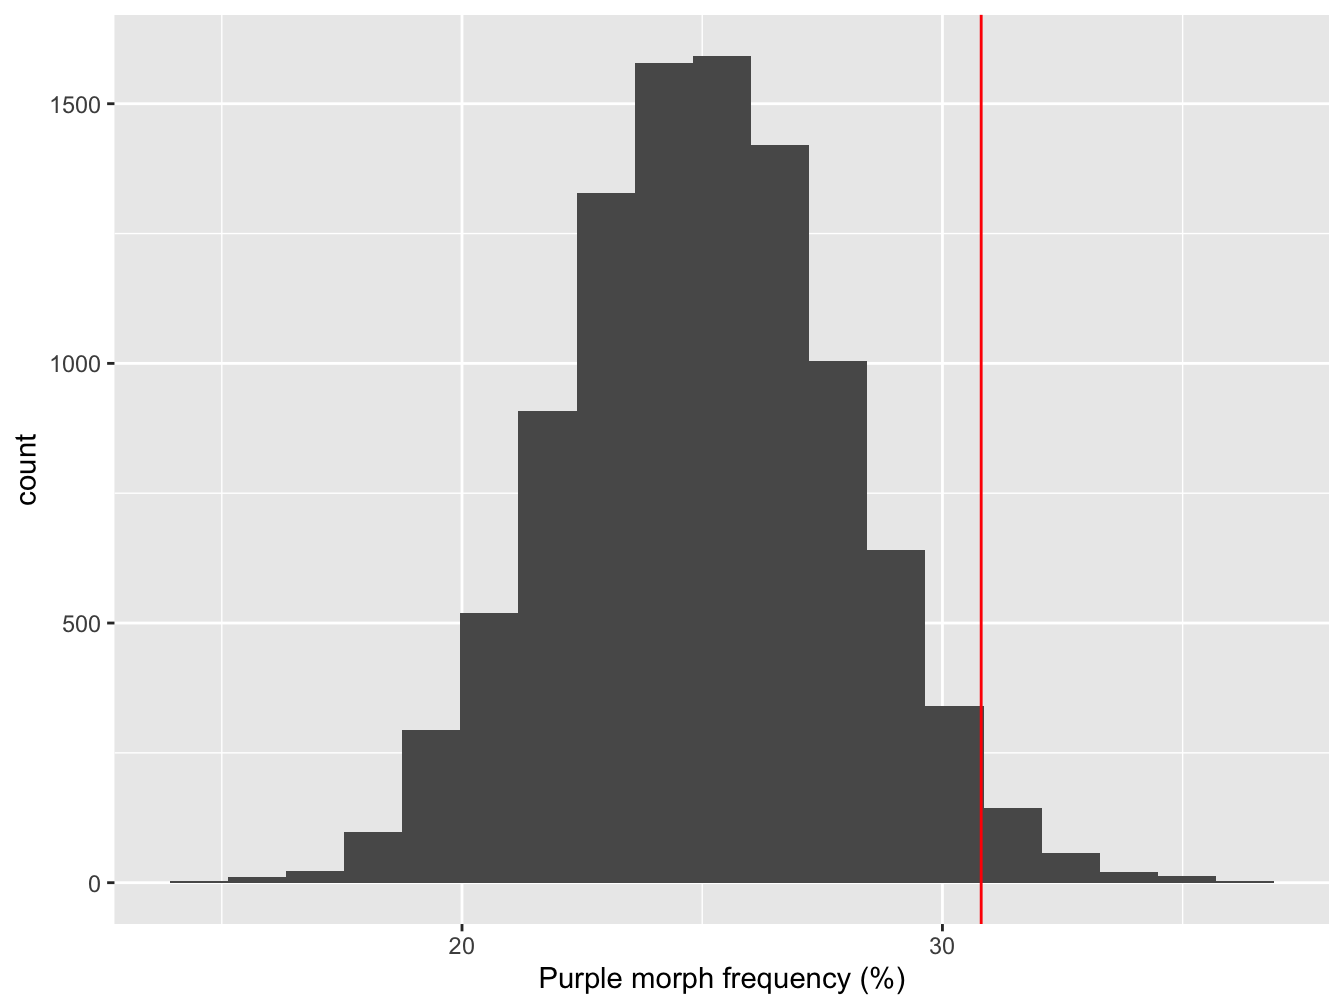
\includegraphics[width=0.75\linewidth]{intro-bio-stats-book_files/figure-latex/boot-samp-dist-25-1} 

}

\caption{Sampling distribution of purple morph frequency under the null hypothesis}\label{fig:boot-samp-dist-25}
\end{figure}

The red line shows where the point estimate from the true sample lies. What does this tells us? It looks like the observed purple morph frequency would be quite unlikely to have arisen through sampling variation if the population frequency really was 25\%. We can say this because the observed frequency (red line) lies at the end of one `tail' of the sampling distribution over on the right.

We need to be able to make a more precise statement than this though. Instead of `eyeballing' the distribution, we can quantify how often the values of the bootstrapped null distribution ended up greater than the observed estimate:

\begin{Shaded}
\begin{Highlighting}[]
\NormalTok{p\_value }\OtherTok{\textless{}{-}} \FunctionTok{sum}\NormalTok{(null\_dist }\SpecialCharTok{\textgreater{}}\NormalTok{ mean\_point\_est) }\SpecialCharTok{/}\NormalTok{ n\_samp}
\NormalTok{p\_value}
\end{Highlighting}
\end{Shaded}

\begin{verbatim}
## [1] 0.0238
\end{verbatim}

This number (generally denoted `\emph{p}') is called a \textbf{\emph{p}-value}.

\hypertarget{interpreting-the-p-value}{%
\subsection*{Interpreting the p-value}\label{interpreting-the-p-value}}
\addcontentsline{toc}{subsection}{Interpreting the p-value}

What are we supposed to do with the finding \emph{p} = 0.0238? This is the probability of obtaining a result equal to, or `more extreme', than that which was actually observed, \emph{assuming that the hypothesis under consideration (the null hypothesis) is true}. The null hypothesis is an hypothesis of no effect (or no difference), and so a low \emph{p}-value can be interpreted as evidence for an effect being present.

It's worth reading that a few times because it is not at all intuitive\ldots{}

In our example, it appears that the purple morph frequency we observed is fairly unlikely to occur if its frequency in the new population really was 25\%. In biological terms, we take the low \emph{p}-value as evidence for a difference in purple morph frequency among the populations, i.e.~the data support the prediction that the purple morph is present at a frequency greater than 25\% in the new study population.

One important question remains: How small does a \emph{p}-value have to be before we are happy to conclude that the effect we're interested in is probably present? In practice, we do this by applying a threshold, called a \textbf{significance level}. If the \emph{p}-value is less than the chosen significance level, we say the result is said to be \textbf{statistically significant}. Very often, we use a significance level of \emph{p} \textless{} 0.05 (5\%).

Why do we use a significance level of \emph{p} \textless{} 0.05? The short answer is that this is just a convention. Nothing more. There is nothing special about the 5\% threshold other than the fact that it's the one most often used. Statistical significance has nothing to do with biological significance. Unfortunately, many people are very uncritical about their use of this arbitrary threshold, to the extent that it can be very hard to publish a scientific study if it doesn't contain `statistically significant' results.

\hypertarget{concluding-remarks}{%
\section{Concluding remarks}\label{concluding-remarks}}

We just carried out a type of statistical test called a \textbf{significance test}. It was a bit convoluted reasoning, but the chain of reasoning we just employed underlies all the significance tests we use in this book. The precise details of how to construct such tests will vary from one problem to the next, but ultimately, when using frequentist ideas we always\ldots{}

\begin{enumerate}
\def\labelenumi{\arabic{enumi}.}
\item
  assume that there is actually no `effect' (the \textbf{null hypothesis}), where an effect is expressed in terms of one or more population parameters,
\item
  construct the corresponding \textbf{null distribution} of the estimated parameter by working out what would happen if we were to take frequent samples in the `no effect' situation,
\end{enumerate}

(This is why the word `frequentist' is used to describe this flavour of statistics.)

\begin{enumerate}
\def\labelenumi{\arabic{enumi}.}
\setcounter{enumi}{2}
\tightlist
\item
  then compare the estimated population parameter to the null distribution to arrive at a \textbf{\emph{p}-value}, which evaluates how frequently the result, or a more extreme result, would be observed under the hypothesis of no effect.
\end{enumerate}

We used the bootstrap to operationalise that process for our example (i.e.~make it real). Bootstrapping is certainly a useful tool, but it is also an advanced technique that can be difficult to apply in many settings. We won't use it anymore---the bootstrap was introduced here to demonstrate how frequentist reasoning works.

We will focus on simple, `off-the-shelf' statistical tools in this book. The good news is we don't need to understand the low-level details to use these tools effectively. As long as we can identify the null hypothesis and understand how to interpret the associated \emph{p}-values we should be in a good position to apply them. These two ideas---null hypotheses and \emph{p}-values---are so important, we're going to consider them in much greater detail over the next two chapters.

\hypertarget{statistical-comparisons}{%
\chapter{Statistical comparisons}\label{statistical-comparisons}}

\hypertarget{making-comparisons}{%
\section{Making comparisons}\label{making-comparisons}}

Scientific inquiry often requires us to evaluate predictions about differences between populations. The simplest such case involves just two populations, e.g.

`Does enzyme activity differ among control and drug-treated cell lines?'

`Do maize plants photosynthesise at different rates at 25°C and 20°C?'

`Do purple and green plants differ in their biomass?'

In this setting, we're evaluating whether or not two \emph{statistical populations} are different in some way. To do this, we have to step through the same kind of process discussed in the last few chapters.

This chapter demonstrates how to compare two populations by employing ideas like null hypotheses and \emph{p}-values. The goal is not really to learn how to compare populations---instead, we want to continue developing our understanding of significance tests and evaluate predictions.

As we do this, we're going to introduce a new component of the frequentist machine called a `test statistic'. This is an important idea---it will crop up every time we introduce a new type of statistical test.

\hypertarget{morph-weights-eg}{%
\subsection{A new example}\label{morph-weights-eg}}

Let's continue with the familiar purple and green plants example. This time, instead of working with morph frequencies, we'll consider plant size. We introduce this by stepping through the process introduced in the \protect\hyperlink{learning-from-data}{learning from data} chapter:

\textbf{Question, hypothesis and prediction:} We think the purple and green morph plants might be different in some way. Specifically, we want to address the question: Why have the purple morphs increased in frequency in the new population? Our working hypothesis is that purple plants are fitter than green plants. Since fitness is closely related to seed production, and seed production is typically positively correlated with plant size, we predict that purple morphs should be larger in the new population.

\textbf{Statistical populations:} What statistical populations are we interested in? This time, we will conceive of each morph as its own statistical population. That means there are now two distinct statistical populations in play: a purple plant population and a green plant population. This change of focus from our earlier analysis where we considered all the plants as one population is perfectly valid. Statistical populations are not really fixed things---they are defined by the problem we're tackling.

\textbf{Variables:} Which variable should we study? An obvious way to address a prediction of size differences of plants is to measure the weight of individuals of each morph in our samples. To be more precise, `dry weight biomass' is the standard, reliable measure of how `big' a plant is. Dry weight mass is a numeric variable measured on a ratio scale (zero means `nothing').

\textbf{Population parameters:} We predict that purple morphs are larger than green morphs. What do we mean by that? We probably don't mean that every purple plant is bigger than every green plant. Instead, we need to know if purple plants are \emph{generally} bigger than green ones. This is a statement about `central tendency'---we want to evaluate whether purple plants are larger than green plants, \emph{on average}. The population parameters of interest are, therefore, the \emph{mean} dry weights of each morph.

\textbf{Gather samples:} The next step is to gather appropriate samples. Since this is a made-up example, we'll cut to the chase. We have already seen the samples we're going to use. When we read in the `MORPH\_DATA.CSV' in the previous chapter, we found a numeric variable called \texttt{Weight}. This contains our dry weight biomass information. The categorical \texttt{Colour} variable analysed in the last chapter tells us which kind of colour morph each observation corresponds to.

Now we're ready to tackle the remaining steps in the `learning from data' process: estimating the population parameter(s), estimating uncertainty, and answering the question. We work through each of these steps in detail next.

\begin{infobox}{action}

\hypertarget{section-1}{%
\subsubsection*{}\label{section-1}}
\addcontentsline{toc}{subsubsection}{}

Once again, the best way to understand what follows is by working through the example, though you can also make good progress through careful reading. In any case, the code again assumes that `MORPH\_DATA.CSV' has been read into a tibble called \texttt{morph\_data}.

\end{infobox}

\hypertarget{examine-the-data}{%
\subsection{Examine the data}\label{examine-the-data}}

The first step is to calculate point estimates of the mean dry weight of each morph. These are our `best guess' of the population means. It can also be useful to know something about the sample size and variability of dry weight in each sample. We can summarise variability using the standard deviation (\texttt{sd}) of each sample. Here is how to do this with \textbf{dplyr}:

\begin{Shaded}
\begin{Highlighting}[]
\CommentTok{\# using morph data...}
\NormalTok{morph\_data }\SpecialCharTok{\%\textgreater{}\%} 
  \CommentTok{\# ...group the data by colour morph category}
  \FunctionTok{group\_by}\NormalTok{(Colour) }\SpecialCharTok{\%\textgreater{}\%} 
  \CommentTok{\# ... calculate the mean, sd and sample size of weight in each category}
  \FunctionTok{summarise}\NormalTok{(}\AttributeTok{mean =} \FunctionTok{mean}\NormalTok{(Weight), }
            \AttributeTok{sd =} \FunctionTok{sd}\NormalTok{(Weight),}
            \AttributeTok{samp\_size =} \FunctionTok{n}\NormalTok{())}
\end{Highlighting}
\end{Shaded}

\begin{verbatim}
## # A tibble: 2 x 4
##   Colour  mean    sd samp_size
##   <chr>  <dbl> <dbl>     <int>
## 1 Green   708.  150.       173
## 2 Purple  767.  156.        77
\end{verbatim}

This shows the mean dry weight of the purple morph is indeed greater than that of the green morph. Maybe our hypothesis is true. The standard deviation estimates indicate that the dry weight of purple morphs is also a bit more variable than the green morphs.

These numbers are point estimates taken from limited samples. If we sampled the populations again, sampling variation would lead to different estimates. We're not yet in a position to conclude that purple morphs are bigger than green morphs because we don't know if the difference is just down to `luck'.

We should also visualise the sample distributions of colour morph weights. We could do this in a variety of ways but since we only have two samples we may as well use a fairly information-rich summary. Histograms are a good choice when we have a reasonable amount of data:

\begin{Shaded}
\begin{Highlighting}[]
\FunctionTok{ggplot}\NormalTok{(morph\_data, }\FunctionTok{aes}\NormalTok{(}\AttributeTok{x =}\NormalTok{ Weight)) }\SpecialCharTok{+} 
  \FunctionTok{geom\_histogram}\NormalTok{(}\AttributeTok{binwidth =} \DecValTok{50}\NormalTok{) }\SpecialCharTok{+} 
  \FunctionTok{facet\_wrap}\NormalTok{(}\SpecialCharTok{\textasciitilde{}}\NormalTok{Colour, }\AttributeTok{ncol =} \DecValTok{1}\NormalTok{) }\CommentTok{\# \textless{}{-} separate histogram for each colour morph!}
\end{Highlighting}
\end{Shaded}

\begin{figure}

{\centering 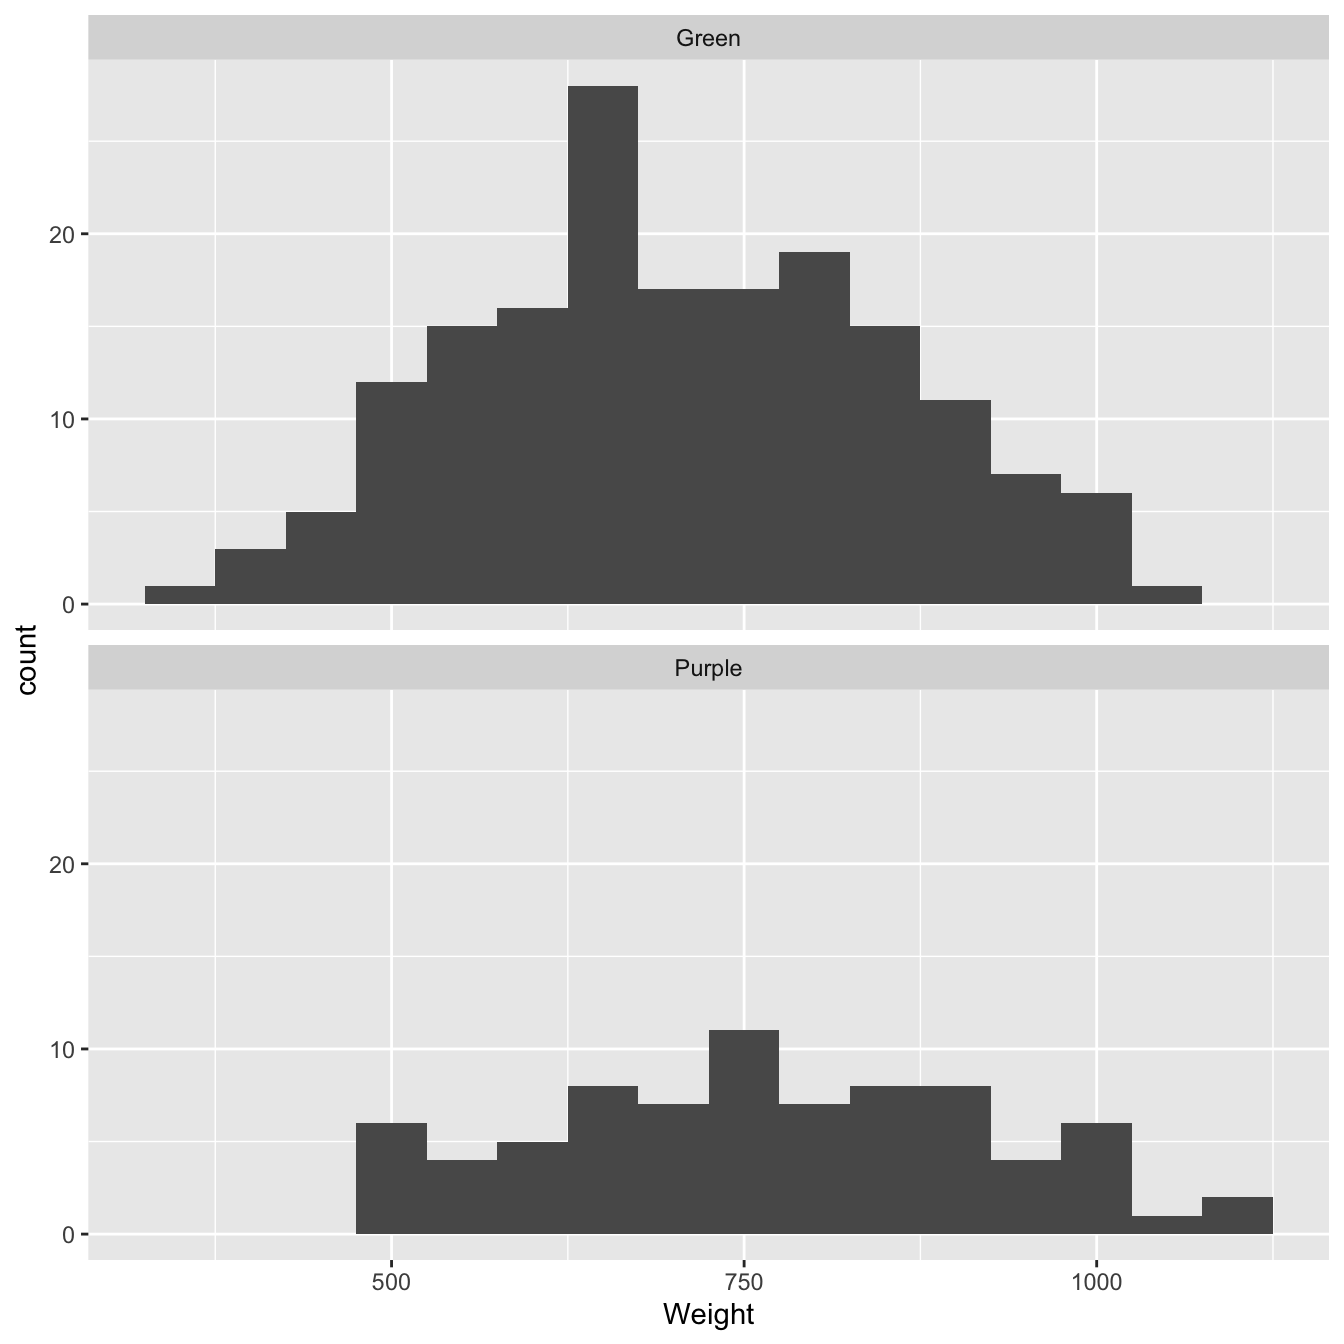
\includegraphics[width=0.75\linewidth]{intro-bio-stats-book_files/figure-latex/two-morph-dist-1} 

}

\caption{Size distributions of purple and green morph samples}\label{fig:two-morph-dist}
\end{figure}

What does this plot tell us? We're interested in the degree of similarity between the two samples. It looks like purple morph individuals tend to have higher dry weights than green morphs. We already knew this, of course. What the plot confirms is that the difference is probably not due to a few extreme cases (`outliers').

It looks like the histograms confirm there might be a general difference in the size of the two morphs. However, there is also a lot of overlap between the two dry weight distributions. Maybe the difference between the sample means is simply a consequence of sampling variation? We need to construct a statistical test to address this question.

\hypertarget{constructing-a-test}{%
\section{Constructing a test}\label{constructing-a-test}}

We will develop a frequentist test to evaluate whether the two population means are likely to be different. Regardless of the precise details, this kind of problem involves a four-step process:

\begin{enumerate}
\def\labelenumi{\arabic{enumi}.}
\item
  First, we \emph{assume} there is no difference between the population means. That is, we hypothesise that all the data are sampled from a pair of populations with the same population mean. To put it another way, we pretend there is really only one population. We know about this trick. It's a statement of the \textbf{null hypothesis}.
\item
  Next, we use information in the real samples to work out what would happen if we were to repeatedly take many new samples in this hypothetical situation of `no difference'. We summarise this by calculating the null distribution of a suitable \textbf{test statistic} (\textless-- this is something new).
\item
  We then ask, ``if there were no difference between the two groups, what is the probability that we would observe a difference that is the same as, or more extreme than, the one we observed in the true sample?'' We know about this number too. It's a \textbf{\emph{p}-value}.
\item
  If the observed difference is sufficiently improbable, we conclude that we have found a \textbf{statistically significant} result. A statistically significant result is one that is inconsistent with the hypothesis of no difference.
\end{enumerate}

This chain of logic is very similar to that used to construct the statistical test in the previous chapter. The main elaboration here is the introduction of the test statistic. When dealing with comparisons involving more than one parameter we need to work with a single numeric summary of `the effect of interest', however defined. Its purpose is to summarise the effect as a single number so that we can construct a statistical test. That's why it is called the `test statistic'.

There are many different kinds of test statistic and many different ways to realise the above process. We're going to use something called a \textbf{permutation test} here. We're not using this because we want to learn how to apply it. Instead, just as with the bootstrap, the permutation test offers a simple way to see how frequentist tests work without getting lost in mathematical detail.

\hypertarget{permutation-tests}{%
\subsection{Permutation tests}\label{permutation-tests}}

A hypothesis of `no difference' between the mean dry weights of purple and green morphs implies the following: the labels `purple' and `green' are meaningless because the two morphs are effectively sampled from the same population. These labels don't carry any real information, meaning they may as well have been randomly assigned to each individual.

This suggests we can evaluate the statistical significance of the observed difference as follows:

\begin{enumerate}
\def\labelenumi{\arabic{enumi}.}
\tightlist
\item
  Make a copy of the original purple and green dry weights sample, but do so by randomly assigning the labels `purple' and `green' to the new copy of the data. Do this in such a way that the original sample sizes are preserved. The process of assigning random labels is called \textbf{permutation}.
\end{enumerate}

(We have to preserve the original sample sizes because we want to mimic the sampling process that we used, i.e.~we want to hold everything constant apart from the labelling of individuals.)

\begin{enumerate}
\def\labelenumi{\arabic{enumi}.}
\setcounter{enumi}{1}
\item
  Repeat the permutation scheme many times until we have a large number of artificial samples; 1000-10000 randomly permuted samples may be sufficient.
\item
  For each permuted sample, calculate whatever test statistic captures the relevant information. In our example, this is the \emph{difference} between the mean dry weight of purple and green morphs in each permuted sample.
\end{enumerate}

(It doesn't matter which way round we calculate the difference.)

\begin{enumerate}
\def\labelenumi{\arabic{enumi}.}
\setcounter{enumi}{3}
\tightlist
\item
  Compare the observed test statistic from the real sample to the distribution of sample statistics from the randomly permuted samples.
\end{enumerate}

This scheme is called a permutation test because it involves random permutation of the group labels. Why is this useful? \emph{Each unique random permutation yields an observation from the null distribution of the difference among sample means, under the assumption that this difference is zero in the population.} We can use this to assess whether or not the observed difference is consistent with the hypothesis of no difference by looking at where it lies relative to this null distribution.

\hypertarget{carrying-out-a-permutation-test}{%
\subsection{Carrying out a permutation test}\label{carrying-out-a-permutation-test}}

It's easy to implement a permutation test in R. We won't show the code this time because it uses quite a few tricks that won't be needed again. It is worth having a quick look at the permuted samples, though. The first 40 values are:

\emph{Sample 1-}

\begin{verbatim}
##     Green    Purple    Purple     Green     Green    Purple     Green    Purple 
##  714.3592  693.4924  556.2063  653.6619  672.5207  661.0097  445.1001  481.5068 
##     Green     Green     Green     Green    Purple    Purple     Green     Green 
##  647.6679  858.4820  567.4104  597.1629  718.7132  539.8551  753.0170  807.7700 
##    Purple    Purple     Green     Green     Green     Green     Green     Green 
## 1085.7036  926.4972  617.1209  632.5897  859.7013  815.4634  666.7693  573.5907 
##     Green     Green    Purple     Green    Purple    Purple     Green     Green 
##  694.2877  836.6883  665.8489  617.7895  590.5936  775.8980  686.6790  813.4272 
##     Green     Green     Green    Purple     Green     Green     Green    Purple 
##  506.3904  566.9971  629.5894  878.2477  823.1128  542.7877  507.7345  786.2809
\end{verbatim}

\emph{Sample 2-}

\begin{verbatim}
##    Purple     Green     Green     Green     Green     Green    Purple    Purple 
##  714.3592  693.4924  556.2063  653.6619  672.5207  661.0097  445.1001  481.5068 
##    Purple     Green     Green    Purple    Purple     Green    Purple     Green 
##  647.6679  858.4820  567.4104  597.1629  718.7132  539.8551  753.0170  807.7700 
##    Purple     Green     Green     Green    Purple    Purple     Green    Purple 
## 1085.7036  926.4972  617.1209  632.5897  859.7013  815.4634  666.7693  573.5907 
##    Purple     Green     Green    Purple     Green     Green     Green     Green 
##  694.2877  836.6883  665.8489  617.7895  590.5936  775.8980  686.6790  813.4272 
##    Purple     Green     Green     Green    Purple     Green     Green    Purple 
##  506.3904  566.9971  629.5894  878.2477  823.1128  542.7877  507.7345  786.2809
\end{verbatim}

The data from each permutation are stored as numeric vectors, where each element of the vector is named according to the morph type it corresponds to---these are `the labels' referred to above. The set of numbers does not vary among permuted samples. The \emph{only} difference between them is the labelling which has been randomly assigned in each permuted sample.

The difference between the mean dry weights in the first permutation is 4.0700017, while in the second sample, the difference is -19.9656492. What matters for our test is the distribution of these differences over the complete set of permutations. This is the approximation to the sampling distribution of the difference between means under the null hypothesis---i.e.~it's our null distribution.

We can visualise this null distribution by making a histogram that summarises the 2500 mean differences from the permuted samples:

\begin{figure}

{\centering 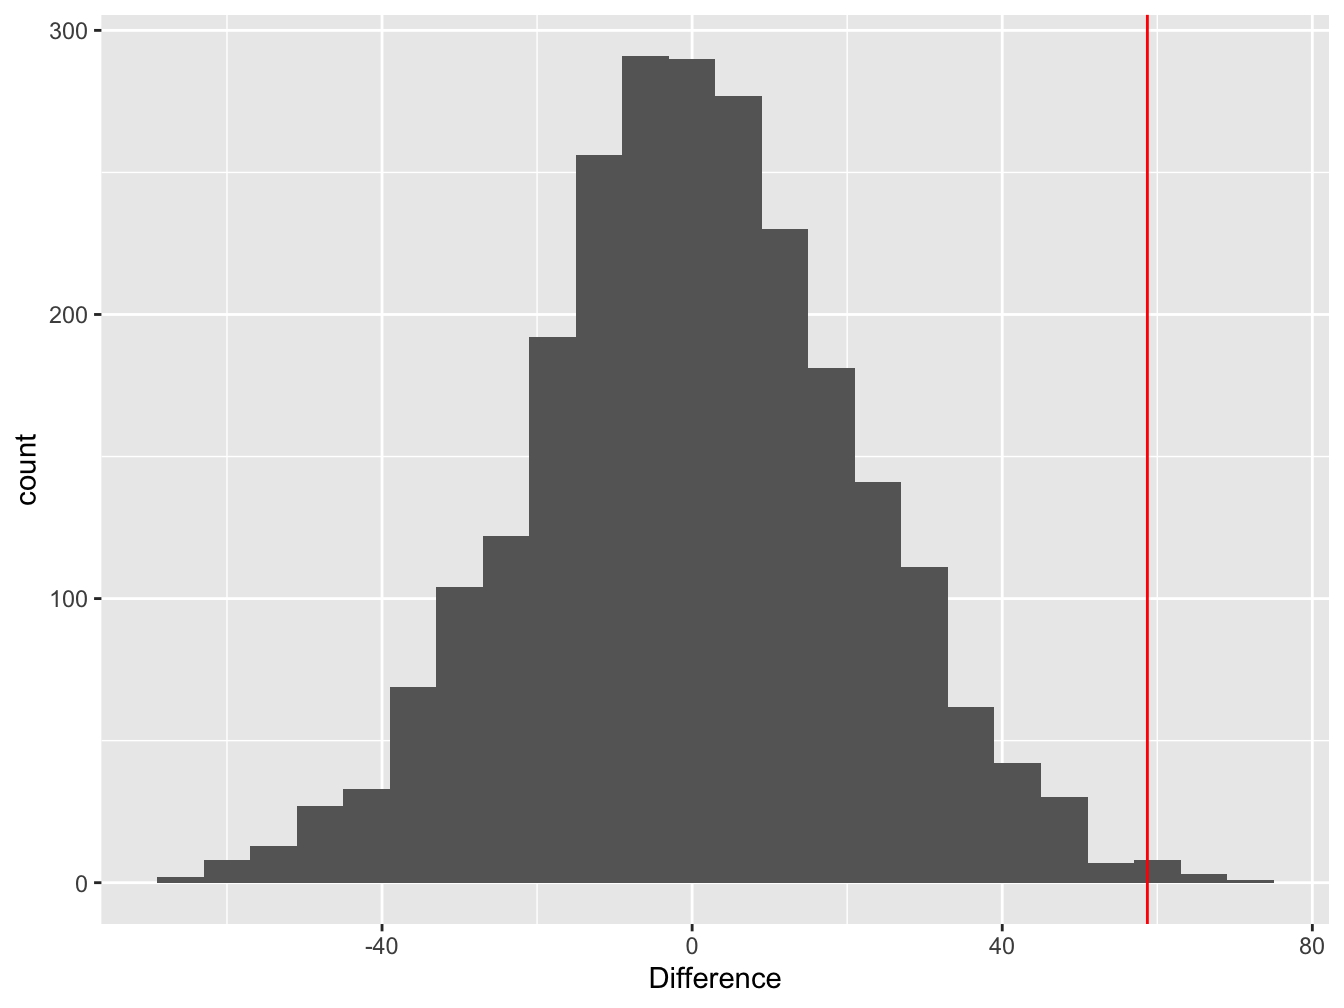
\includegraphics[width=0.8\linewidth]{intro-bio-stats-book_files/figure-latex/permute-dist-1} 

}

\caption{Difference between means of permuted samples}\label{fig:permute-dist}
\end{figure}

Notice that the distribution is centred at zero. This makes perfect sense---if we take a set of numbers and randomly allocate them to groups, on average, we expect the difference between the means of the groups to be zero.

The red line shows the estimated difference between the mean purple and green morph dry weights \emph{in the real sample}. This is the test statistic. The key thing to notice here is the location of the test statistic within the null distribution.

In this example, the estimated difference lies at the end of the right `tail' of the null distribution. What does that tell us? It suggests the observed difference (the red line) is unlikely to arise through pure sampling variation if the two population means were identical.

So\ldots{} it looks like the data are inconsistent with the null hypothesis of no difference. What we need is a number to quantify this inconsistency---the all-important \emph{p}-value.

\hypertarget{calculating-the-p-value}{%
\subsection*{\texorpdfstring{Calculating the \emph{p}-value}{Calculating the p-value}}\label{calculating-the-p-value}}
\addcontentsline{toc}{subsection}{Calculating the \emph{p}-value}

We use the null distribution to quantify the probability of ending up with the observed difference under the null hypothesis. Only 10 out of the 2500 permutations ended up being equal to, or `more extreme' (more positive) than, the observed difference. This means the probability of finding a difference in the means equal to, or more positive than, the observed difference is about, \emph{p} = 10/2500 = 0.004. This is the \emph{p}-value for our significance test.

Let's run through the interpretation of that \emph{p}-value. Here's the general chain of logic again\ldots{} The \emph{p}-value is the probability of obtaining a test statistic equal to, or `more extreme' than, the estimated value, assuming the null hypothesis is true. The null hypothesis is one of no effect, so a small \emph{p}-value can be interpreted as evidence for the effect (e.g.~a difference between means) being present. That's a weird way to seek evidence for the presence of an effect, but that's how frequentist statistics works.

How low does the \emph{p}-value actually have to be before we decide we have `enough evidence'? Less than 0.01? Less than 0.001? Any threshold is somewhat arbitrary to be honest, but in biology, a significance threshold of \emph{p} \textless{} 0.05 is conventionally used. If we find \emph{p} \textless{} 0.05, then we conclude that we found a `statistically significant' effect at the 5\% level.

Here's how this logic applies to our example\ldots{} The permutation test assumed there was no difference between the purple and green morphs, so the low \emph{p}-value indicates that the estimated difference between the mean dry weight of purple and green morphs was unlikely to have occurred by chance \emph{if} there is really no difference at the population level. We interpret the low \emph{p}-value as evidence for the existence of a difference in mean dry weight among the populations of purple and green morphs. Since \emph{p} = 0.004, we say we found a statistically significant difference at the 5\% level.

Here's how we might summarise our analysis in in a written report:

\begin{quote}
The mean dry weight biomass of purple plants (77) was significantly greater than that of green plants (173) (one-tailed permutation test, p\textless0.05).
\end{quote}

We report the sample sizes used, the type of test employed, and the significance threshold we passed (not the raw \emph{p}-value).

\begin{infobox}{information}

\hypertarget{directional-tests}{%
\subsubsection*{Directional tests}\label{directional-tests}}
\addcontentsline{toc}{subsubsection}{Directional tests}

The test we just did is a `one-tailed' test. It's called a `one-tailed' because we only looked at one end of the null distribution. This kind of test is appropriate for evaluating directional predictions (e.g.~purple \textgreater{} green). If, instead of testing whether purple plants were larger than green plants, we just want to know if they were different in some way (i.e.~in either direction), we should use a `two-tailed' test. These work by looking at both ends of the null distribution. We won't do this here though---the one- vs two-tailed distinction is discussed in the \protect\hyperlink{one-two-tailed-tests}{one-tailed vs.~two-tailed tests} supplementary chapter.

\end{infobox}

\hypertarget{what-have-we-learned}{%
\section{What have we learned?}\label{what-have-we-learned}}

Our goal was not really to learn how permutation tests work. Just as with bootstrapping in the previous chapter---we just used it to demonstrate the logic of how frequentist statistics work. In this instance, we wanted to see how to evaluate a difference between two groups. The basic ideas are no different from those introduced in the previous chapter\ldots{}

\begin{enumerate}
\def\labelenumi{\arabic{enumi}.}
\item
  define what constitutes an `effect' (e.g.~a difference between means), then assume that there is `no effect'---i.e.~define the \textbf{null hypothesis},
\item
  select an appropriate \textbf{test statistic} that can distinguish between the presence of an `effect' and `no effect',
\end{enumerate}

(In practice, each kind of statistical test uses a standard test statistic. We don't have to pick these ourselves.)

\begin{enumerate}
\def\labelenumi{\arabic{enumi}.}
\setcounter{enumi}{2}
\item
  construct the corresponding \textbf{null distribution} of the test statistic by working out what would happen if we were to take frequent samples in the `no effect' situation,
\item
  and finally, use the null distribution and the observed test statistic to calculate a \_\_\emph{p}-value\_\_that quantifies how frequently the observed difference, or a more extreme difference, would be observed under the hypothesis of no effect.
\end{enumerate}

We only actually introduced one new idea in this chapter. When evaluating differences among populations, we need to work with a single number that can distinguish between `effect' and `no effect'. This is called the test statistic. Sometimes this can be expressed in terms of familiar quantities like means (we just used a difference between means above). However, this isn't always the case. For example, we can use something called an \emph{F}-ratio to evaluate the statistical significance of differences among more than two means. We'll get to these kinds of tests later. For now, our task is to explore simple `parametric tests'. These kinds of tests allow us to ask questions without resorting to things bootstrapping or permutation tests.

\hypertarget{hypotheses-and-p-values}{%
\chapter{\texorpdfstring{Hypotheses and \emph{p}-values}{Hypotheses and p-values}}\label{hypotheses-and-p-values}}

\begin{figure}

{\centering 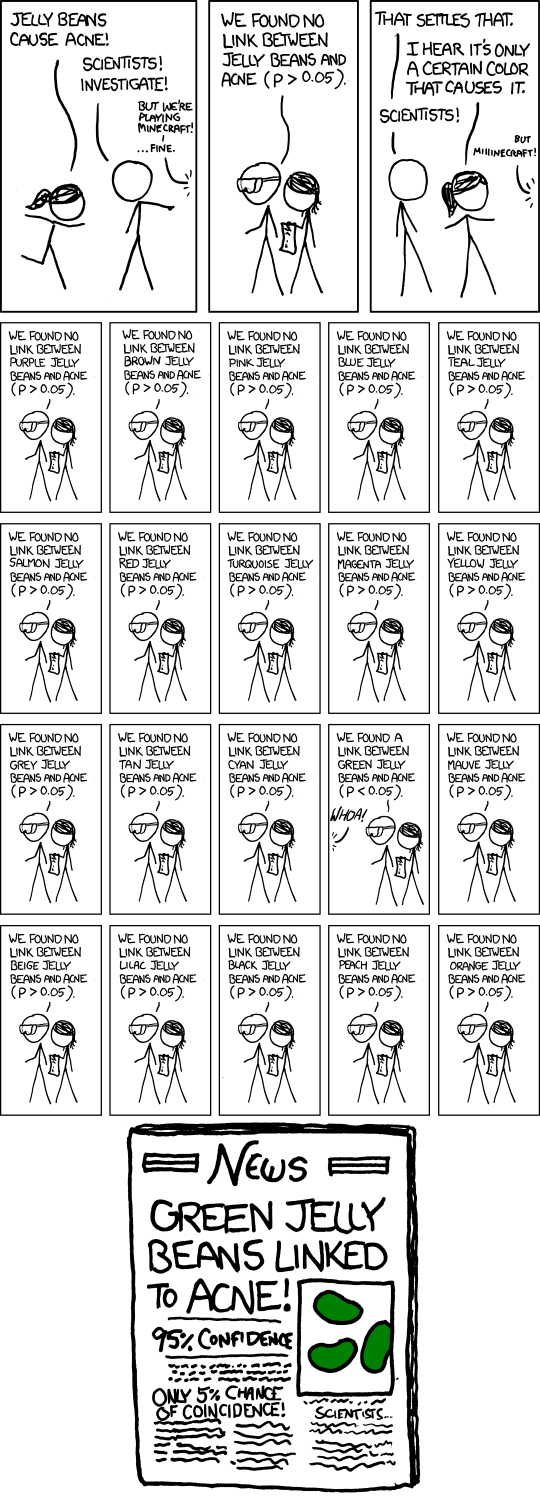
\includegraphics[width=0.5\linewidth]{./images/significant_xkcd} 

}

\caption{Significant: [xkcd.com](https://xkcd.com/882)}\label{fig:jellybeans}
\end{figure}

\hypertarget{a-few-words-about-the-null-hypothesis}{%
\section{A few words about the null hypothesis}\label{a-few-words-about-the-null-hypothesis}}

When using frequentist statistics, we are always asking what would happen if we continually sampled from a population \emph{where the effect we are interested in is not present}. This idea of an hypothetical `no effect' situation is so important that it has a special name; it is called \textbf{the null hypothesis}. Every kind of statistical test (in this book at least) works by first specifying a particular null hypothesis. It is hard to understand a statistical test's result if we don't know its null hypothesis.

\hypertarget{hypotheses-and-null-hypotheses}{%
\subsection{Hypotheses and null hypotheses}\label{hypotheses-and-null-hypotheses}}

When discussing \protect\hyperlink{stages-hypotheses}{the scientific process}, we said that an hypothesis is a statement of a proposed process or mechanism responsible for an observed pattern or effect. We have also seen that in statistics, we encounter `hypothesis' used differently. In particular, we often see \textbf{null hypotheses} (often written in statistics books as H\textsubscript{0}).

The null hypothesis is a statement of what we would expect to see if there is no effect of the factor we are looking at (e.g., plant morphology) on the variable that we measure (e.g., dry weight biomass). So in the second plant morph example, our null hypothesis was \emph{There is no difference in mean biomass of purple and green plants}. All frequentist statistical tests work by specifying a null hypothesis and then evaluating the observed data to see if they deviate from the null hypothesis in a way that is inconsistent with sampling variation. This may seem like a rather odd approach, but this is how frequentist tests work.

It is important to be aware of what a null hypothesis is, and what it is used for, so that we can interpret the results of statistical tests. However, in a general discussion of an analysis, we normally refer to the effect we are actually interested in. This is called the \emph{test hypothesis} or the \emph{alternative hypothesis} (often denoted H\textsubscript{1} in statistics books). The alternative hypothesis is essentially a statement of the effect we are expecting (or hoping!) to see, e.g., purple and green plants differ in their mean size. It is a statement of whatever is implied if the null hypothesis is not true.

Having sorted out the different types of hypotheses in play, we can use a particular frequentist technique to evaluate the observed result against that expected if the null hypothesis was true. The test gives us a probability (\emph{p}-value) telling us how likely it is that we would have got the result we observe, or a more extreme result, if the null hypothesis was really true. If the value is sufficiently small we judge it unlikely that we would have seen this result if the null hypothesis was true. Consequently, we say we \emph{reject the null hypothesis} (i.e.~reject the notion that there is no difference). This is not the same as `proving' the alternative hypothesis is true. We can't prove anything by collecting data or carrying out an experiment.

If the \emph{p}-value is large, then it is quite likely that we could have ended up with the observed result if the null hypothesis was true, i.e.~it is probably due to sampling variation. In this case, we cannot reject the null hypothesis. Note that we say that we ``\emph{do not reject the null hypothesis}''. This is not the same as accepting that the null hypothesis is true, paradoxical though this may seem. One possible reason for this is that if we only have a small sample, there may be an effect of the factor we are looking at, but we can't detect it because we don't have enough data.

\begin{infobox}{information}

\hypertarget{a-p-value-is-not-an-evidence-summary}{%
\subsubsection*{\texorpdfstring{A \emph{p}-value is not an evidence summary}{A p-value is not an evidence summary}}\label{a-p-value-is-not-an-evidence-summary}}
\addcontentsline{toc}{subsubsection}{A \emph{p}-value is not an evidence summary}

A null hypothesis significance test gives us a probability (the \emph{p}-value) of how likely it is that we would have got the result we observe, or a more extreme result, if the null hypothesis was true. The `result' is a property of the data and the test describes how likely the data are under a null hypothesis. A \emph{p}-value is \textbf{not} a measure of evidence in the conventional sense or a statement about the likelihood that any particular hypothesis is true or not.

\end{infobox}

\hypertarget{report-the-null-hypothesis}{%
\subsection{Report the null hypothesis?}\label{report-the-null-hypothesis}}

It's important to realise that we \textbf{do not report null hypotheses when communicating science}. The null hypothesis is nothing more a device for setting up a frequentist statistical test. It is not an interesting or useful hypothesis in its own right. Again, for the avoidance of doubt\ldots{} there's absolutely no need to state the null hypothesis of each and every test we use in a report or a presentation. Focus on substantive biological hypotheses instead.

\hypertarget{interpreting-and-reporting-p-values}{%
\section{\texorpdfstring{Interpreting and reporting \emph{p}-values}{Interpreting and reporting p-values}}\label{interpreting-and-reporting-p-values}}

It is important to understand the meaning of the probabilities generated by frequentist tests. We have already said a \emph{p}-value is the proportion of occasions on which we would expect to see a result at least as extreme as the one you actually observed if the null hypothesis (of no effect) was true. Conventionally, we accept a result as statistically significant if \emph{p} \textless{} 0.05 (also expressed as 5\%). This threshold is called the \textbf{significance level} of a test. We've said it before, but it is worth repeating: there is nothing special about the \emph{p} \textless{} 0.05 significance level! It is just a widely used convention.

\begin{infobox}{warning}

\hypertarget{section-2}{%
\subsubsection*{}\label{section-2}}
\addcontentsline{toc}{subsubsection}{}

We will always use the \emph{p} = 0.05 threshold in this book. Try to remember this---we won't constantly remind you of it. Why use that significance level? There's no particularly special reason. We're simply following a somewhat arbitrary convention that applies to simple analyses of small datasets.

\end{infobox}

A probability of 0.05 is a chance of 1 in 20. This means that if there really was no effect of the factor we are investigating, we would expect to get a result significant at \emph{p}=0.05 about 5 times in 100 samples. To envisage it more easily, it is slightly less than the chance of tossing a coin 4 times and getting 4 heads in a row (\emph{p}=0.0625). It's not all that rare, really. This puts a `significant' result into context. Would we launch a new drug on the market on the evidence of the strength of four heads coming up in a row when a coin is tossed? Probably not!

\hypertarget{careful-with-those-p-values}{%
\subsection{\texorpdfstring{Careful with those \emph{p}-values}{Careful with those p-values}}\label{careful-with-those-p-values}}

This is a good time to issue an important warning about \emph{p}-values. Frequentist \emph{p}-values are counter-intuitive quantities that are easily (and often) misinterpreted. Whole books have been written about the problems associated with them. We don't have time to really cover the issues here, but here are a few key observations:

\begin{itemize}
\item
  Scientists tend to use \emph{p}=0.05 to define `significance', but \emph{p}=0.055 is really no different from \emph{p}=0.045. It would be irrational to reject an idea completely just on the basis of a result of \emph{p}=0.055, while at the same time being prepared to invest large amounts of time and money implementing policies based on a result of \emph{p}=0.045.
\item
  The exact value of \emph{p} is affected by the size of the true effect being studied, the amount of data being analysed, and how appropriate a statistical model is for those data. It's very easy to arrive at a tiny \emph{p}-value, when an effect is weak or even absent, by using a statistical model that is inappropriate for the data in hand.
\item
  A significance test works out how likely our data are under a null hypothesis. The resulting \emph{p}-value is not a measure of evidence or a statement about the likelihood a hypothesis is true or not. That's a shame, because those latter kinds of probabilities are the sort of thing most of us have in mind when we think about evaluating hypotheses. That doesn't change the fact that a \emph{p}-value is not the thing we want it to be!
\item
  A consequence of the previous point is that the relationship between the `strength of an effect' and its associated \emph{p}-value is complicated. It is simply not correct to equate the size of a \emph{p}-value with the weight of evidence for the effect being present, nor is correct to interpret a \emph{p}-value a statement about how big the effect is.
\end{itemize}

The take-home message: \emph{p}-values are hard to interpret and only represent one possible (non-intuitive) source of information when answering scientific questions. They are not the `final word' on truth.

\hypertarget{presenting-p-values}{%
\subsection{\texorpdfstring{Presenting \emph{p}-values}{Presenting p-values}}\label{presenting-p-values}}

R will typically display \emph{p}-values from a statistical significance test to six decimal places (e.g.~\emph{p} = 0.003672). However, when we write about them, the results from tests are usually presented as one of the following four categories:

\begin{itemize}
\item
  \emph{p} \textgreater{} 0.05, for results which are not statistically significant (sometimes also written as `NS'),
\item
  \emph{p} \textless{} 0.05, for results where 0.01 \textless{} \emph{p} \textless{} 0.05,
\item
  \emph{p} \textless{} 0.01, for results where 0.001 \textless{} \emph{p} \textless{} 0.01,
\item
  \emph{p} \textless{} 0.001 for results where \emph{p} \textless{} 0.001,
\end{itemize}

This presentation stems from the fact that statistical tests often had to be calculated by hand in the days before everyone had access to a computer. The significance of the result was difficult to calculate directly, so it would have been looked up in a special table. We still use this style because the value of \emph{p} does not have a simple interpretation in terms of weight of evidence or effect sizes. Knowing which category a \emph{p}-value falls into provides sufficient information to roughly judge `how significant' the result is.

\begin{infobox}{warning}

\hypertarget{significance-thresholds-vs.-p-values}{%
\subsubsection*{\texorpdfstring{Significance thresholds vs.~\emph{p}-values}{Significance thresholds vs.~p-values}}\label{significance-thresholds-vs.-p-values}}
\addcontentsline{toc}{subsubsection}{Significance thresholds vs.~\emph{p}-values}

The significance level is used to determine whether or not a result is deemed to be `statistically significant'. We use \emph{p} \textless{} 0.05 in this book, and we will generally adopt the above categories to report the results of a test. Don't confuse the category used to report the \emph{p}-value with the actual significance level an investigator is using. Just because someone writes `\emph{p} \textless{} 0.01' when they report the results of a test, it does not mean that they were working at the 1\% significance level (\emph{p} = 0.01).

\end{infobox}

It's usually sufficient to use the four categories above when writing about the significance of a statistical test, though occasionally, giving the actual probability can be appropriate. For example, it can be informative to know that a test yielded \emph{p} = 0.06 rather than simply quoting it just as \emph{p} \textgreater{} 0.05 or NS. This is because \emph{p} is so close to the significance threshold. While not wholly convincing, it is still suggestive of the possibility that an effect is present.

\begin{infobox}{information}

\hypertarget{the-asterisks-convention}{%
\subsubsection*{The asterisks convention}\label{the-asterisks-convention}}
\addcontentsline{toc}{subsubsection}{The asterisks convention}

It is common to see ranges of probabilities coded with asterisks in tables and figures:

\begin{itemize}
\tightlist
\item
  \texttt{*} for \emph{p} = 0.05\ldots0.01,
\item
  \texttt{**} for \emph{p} = 0.01\ldots0.001,
\item
  \texttt{***} for \emph{p} \textless{} 0.001.
\end{itemize}

This convention is sometimes used because it offers a compact way to represent the results of a significance test. It's fine to adopt it in tables and figures. However, people do not use the asterisks convention in the text of a report.

\end{infobox}

\hypertarget{biological-vs.-statistical-significance}{%
\section{Biological vs.~statistical significance}\label{biological-vs.-statistical-significance}}

A final, but vital, point: do not confuse statistical significance with biological significance. A result may be statistically highly significant (say \emph{p} \textless{} 0.001) but biologically trivial. To give a real example, in a study of the factors determining the distribution of freshwater invertebrates in a river, the pH of water was measured in the open water and in the middle of the beds of submerged vegetation. There was a statistically significant difference in pH (\emph{p} \textless{} 0.01) but the mean pH values were 7.1 in the open water and 6.9 in the weeds. This is a very small effect, and almost certainly of no importance at all to the invertebrates.

The significance of a result depends on a combination of three things (1) the size of the true effect in the population, (2) the variability of the data, and (3) the sample size. Even a tiny effect can be significant if the sample size is very large. Do not automatically equate a significant result with a large biological effect. Plot the data, inspect the estimates, and consider the biological implications of the difference. The statistical results provide some guidance in separating genuine differences from random variation, but they can't tell us whether the difference is biologically interesting or important---that's the scientist's job!

\hypertarget{part-simple-statistics}{%
\part{Simple Statistics}\label{part-simple-statistics}}

\hypertarget{parametric-statistics}{%
\chapter{Parametric statistics}\label{parametric-statistics}}

\hypertarget{introduction}{%
\section{Introduction}\label{introduction}}

The majority of statistical tools used in this book share one important feature---they are underpinned by a mathematical model of some kind. Because a mathematical model lurks in the background, this particular flavour of statistics called \textbf{parametric statistics}. In this context, the word `parametric' refers to the fact that a mathematical model's behaviour depends on one or more quantities known as `parameters'.

We are \textbf{not} going to study the mathematical details of these models. However, it is important to understand the \textbf{assumptions} underlying a statistical model. Assumptions are the aspects of a system that we accept as true, or at least nearly true. If our assumptions are not reasonable, we can't be sure that the results of our analysis (e.g.~a statistical test) will be reliable. We always need to evaluate the assumptions of an analysis to determine whether or not we trust it.

Ultimately, we want to understand, in approximate terms, how a model and its assumptions lead to a particular statistical test. We have already explored aspects of this process in the last few chapters, such as sampling variation, null distributions, and \emph{p}-values. By thinking about models and their assumptions we can connect these abstract ideas to the practical side of `doing statistics'. Our goal in this chapter is to introduce a few more concepts required to make these connections.

\hypertarget{math-models}{%
\section{Mathematical models}\label{math-models}}

A mathematical model is a description of a system using the language and concepts of mathematics. That `system' could be more or less anything scientists study---the movement of planets in a solar system, the carbon cycle of our planet, changes in abundance and distribution of a species, the development of an organ, or the spread of a plasmid conferring antibiotic resistance.

In the frequentist world, a statistical model is a type of mathematical model that describes how samples of data are generated from a hypothetical population. We're only going to consider only a small subset of the huge array of statistical models people routinely use. Conceptually, the parametric models we use in this book describe data in terms of a \textbf{systematic component} and a \textbf{random component}:

\[\text{Observed Data} = \text{Systematic Component} + \text{Random Component}\] What are these two components?

\begin{itemize}
\item
  The systematic component of a model describes the structure, or the relationships, in the data. When people refer to `the model', this is the bit they usually care about.
\item
  The random component captures the leftover ``noise'' in the data. This is essentially the part of the data that the systematic component of the model fails to describe.
\end{itemize}

This is best understood by example. In what follows, we're going to label the individual values in the sample \(y_i\). The \(i\) in this label indexes the individual values; it takes values 1, 2, 3, 4, \ldots{} and so on. We can think of the collection of the \(y_i\)'s as the variable we're interested in.

The simplest kind of model we might consider is one that describes a single variable. A model for these data can be written: \(y_i = a + \epsilon_i\). In this model:

\begin{itemize}
\item
  The systematic component is given by \(a\). This is usually thought of as the population mean.
\item
  The random component is given by \(\epsilon_i\), which describes how the individual values deviate from the mean.
\end{itemize}

A more complicated model might consider the relationship between the values of \(y_i\) and another variable. We'll call this second variable \(x_i\). A model for these data could be written as: \(y_i = a + b \times x_i + \epsilon_i\). In this model:

\begin{itemize}
\item
  The systematic component is the \(a + b \times x_i\) bit. This is just the equation of a straight line, with intercept \(a\) and slope \(b\).
\item
  The random component is given by the \(\epsilon_i\). Now, this term describes how the individual values deviate from the line.
\end{itemize}

These two descriptions have not yet completely specified our example models. We need to make one more assumption to complete them. The values of the \(\epsilon_i\) differ from one observation to the next because they describe the noise in the system. For this reason, \(\epsilon_i\) is thought of as a statistical variable, which means we also need to specify its \emph{distribution}.

What is missing from our description so far is, therefore, a statement about the distribution of the \(\epsilon_i\). We need to formally set out what kinds of values it is allowed to take and how likely those different values are. The distributional assumption is almost always the same in this book: we assume that the \(\epsilon_i\) are drawn from a \textbf{normal distribution}.

\hypertarget{parametric-stats}{%
\section{The normal distribution}\label{parametric-stats}}

Most people have encountered the normal distribution at one point or another, even if they didn't realise it at the time. Here is a histogram of 100000 values drawn from a normal distribution:

\begin{figure}

{\centering 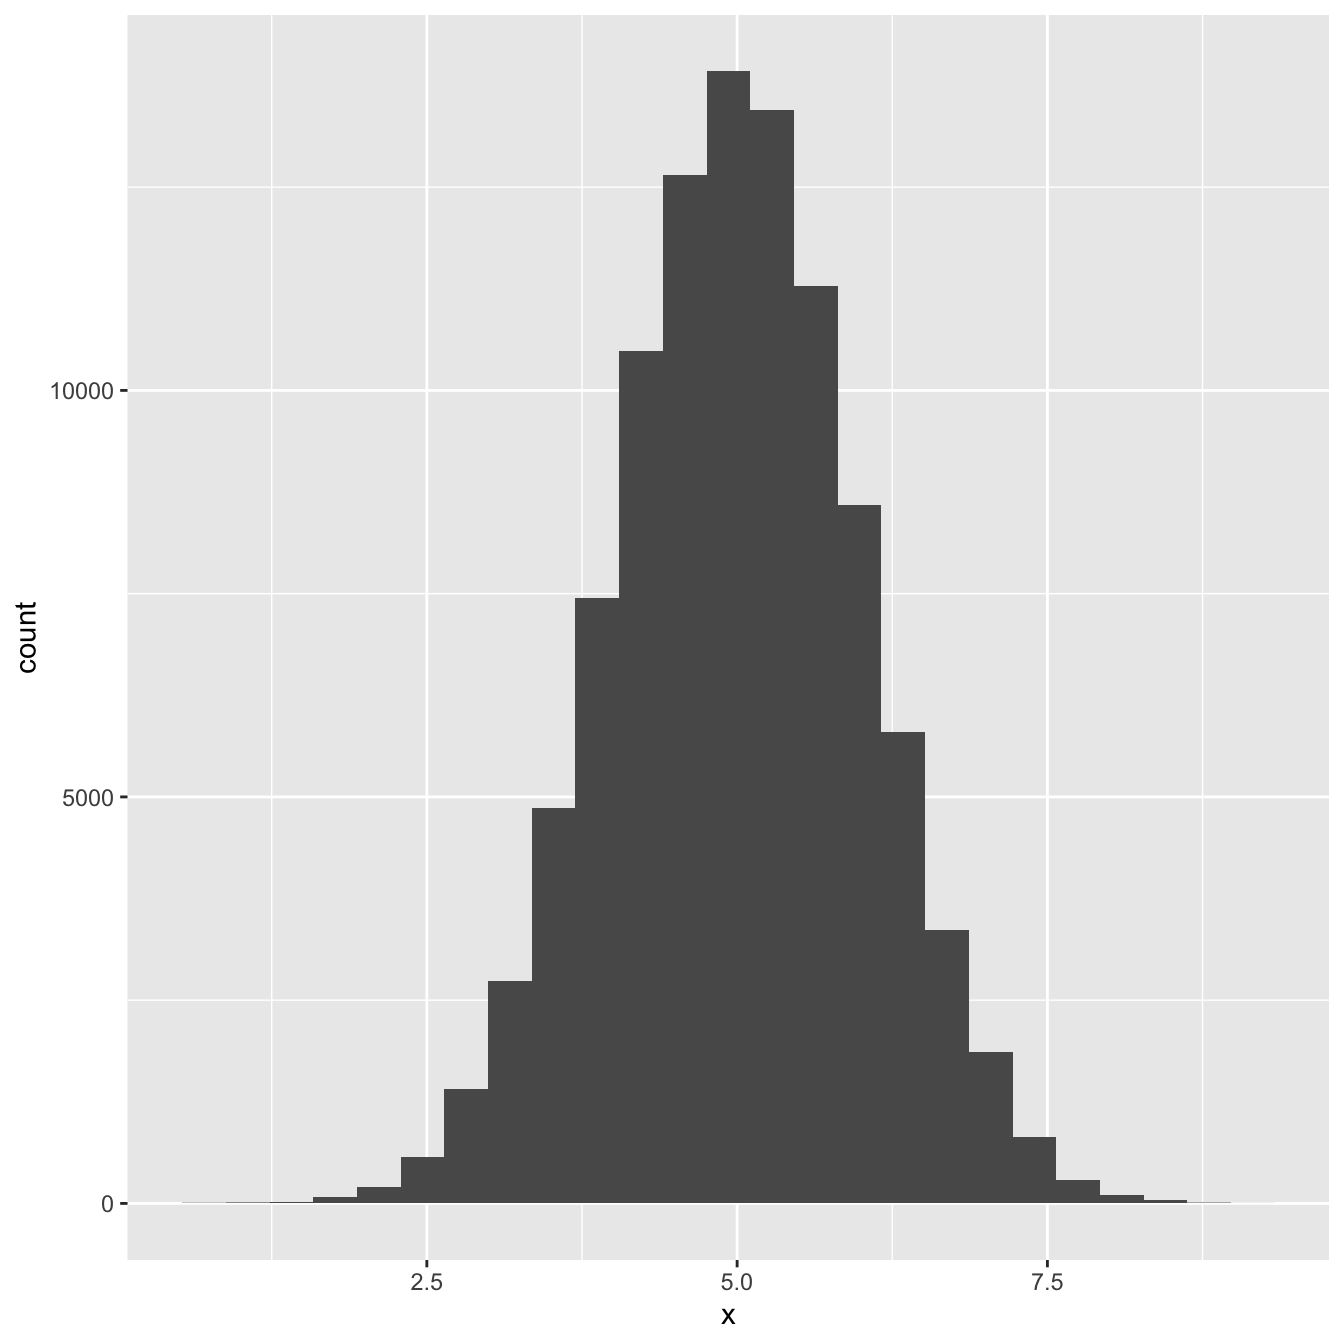
\includegraphics[width=0.6\linewidth]{intro-bio-stats-book_files/figure-latex/norm-dist-eg-1} 

}

\caption{Distribution of a large sample of normally distributed variable}\label{fig:norm-dist-eg}
\end{figure}

Does that look familiar? The normal distribution is sometimes called the `Gaussian distribution', or more colloquially, the `bell-shaped curve'. We don't have time in this book to study this distribution in any detail. Instead, we'll simply list some key facts about the normal distribution that relate to the statistical models we'll be using later on:

\begin{enumerate}
\def\labelenumi{\arabic{enumi}.}
\item
  The normal distribution is appropriate for numeric variables measured on an interval or ratio scale. Strictly speaking, the variable should also be continuous, though a normal distribution can provide a decent approximation for some kinds of discrete numeric data.
\item
  The normal distribution is completely described by its mean (its central tendency) and its standard deviation (its dispersion). If we know these two quantities for a particular normal distribution, we know everything there is to know about that distribution.
\item
  If a variable is normally distributed, then about 95\% of its values will fall inside an interval that is 4 standard deviations wide: the upper bound is equal to the \(\text{Mean} + 2 \times \text{S.D.}\); the lower bound is equal to \(\text{Mean} - 2 \times \text{S.D.}\).
\item
  When we add or subtract two normally distributed variables to create a new variable, the resulting variable will also be normally distributed. Similarly, if we multiply a normally distributed by a number to create a new variable, the resulting variable will still be normally distributed.
\end{enumerate}

The mathematical properties of the normal distribution are very well understood. This has made it possible for mathematicians to determine how the sampling distribution of means and variances behaves when the underlying variables are normally distributed. This knowledge underpins many of the statistical tests we use in this book.

\hypertarget{standard-error-of-the-mean}{%
\subsection{Standard error of the mean}\label{standard-error-of-the-mean}}

Let's consider a simple example. We want to estimate the standard error associated with a sample mean. If we're happy to assume that the sample was drawn from a normal distribution, then there's no need to resort to computationally expensive techniques like bootstrapping to work this out.

There is a well-known formula for calculating the standard error once we assume normality. If \(s^2\) is the variance of the sample, and \(n\) is the sample size, the standard error is given by:

\[\text{Standard error of the mean} = \sqrt{\frac{s^2}{n}}\]

That's it, if we know the variance and the size of a sample, it's easy to estimate the standard error of its mean \emph{if we're happy to assume the sample came from a normally distributed variable}\footnote{In fact, the equation for the standard error of a mean applies when we have a big sample, even if that sample did not come from a normally distributed variable. This result is a consequence of that `the central limit theorem' mentioned in this chapter.}.

In fact, as a result of rule \#4 above, we can calculate the standard error of \emph{any quantity} that involves adding or subtracting the means of samples drawn from normal distributions.

\hypertarget{the-t-distribution}{%
\subsection{\texorpdfstring{The \emph{t} distribution}{The t distribution}}\label{the-t-distribution}}

The normal distribution is usually the first distribution people learn about in a statics course. The reasons for this are:

\begin{itemize}
\tightlist
\item
  it crops up a lot as a consequence of something called `the central limit theorem', and
\item
  many other important distributions are related to the normal distribution in some way.
\end{itemize}

We're not going to worry about the central limit theorem here. However, we do need to consider one more distribution. One of the most important of those `other distributions' is Student's \emph{t}-distribution\footnote{Why is it called Student's \emph{t}? The \emph{t}-distribution was discovered by W.G. Gosset, a statistician employed by the Guinness Brewery. He published his statistical work under the pseudonym of `Student', because Guinness would have claimed ownership of his work if he had used his real name.}.

This distribution arises whenever:

\begin{itemize}
\tightlist
\item
  we take a sample from a normally distributed variable,
\item
  estimate the population mean from the sample,
\item
  and then divide the mean by its standard error.
\end{itemize}

The sampling distribution of this new quantity has a particular form. It follows a Student's \emph{t}-distribution.

Student's \emph{t}-distribution arises all the time in relation to means. For example, what happens if we take samples from a pair of normal distributions, calculate the difference between their estimated means, and then divide this difference by its standard error? The sampling distribution of the scaled difference between means also follows a Student's \emph{t}-distribution.

Because it involves rescaling a mean by its standard error, the form of a \emph{t}-distribution only depends on one thing: the sample size. This may not sound like an important result, but it really is, because it allows us to construct simple statistical tests to evaluate differences between means. We'll be relying on this result in the next two chapters as we learn about so-called `\emph{t}-tests'.

\hypertarget{one-sample-t-tests}{%
\chapter{\texorpdfstring{One sample \emph{t}-tests}{One sample t-tests}}\label{one-sample-t-tests}}

\hypertarget{when-do-we-use-a-one-sample-t-test}{%
\section{\texorpdfstring{When do we use a one-sample \emph{t}-test?}{When do we use a one-sample t-test?}}\label{when-do-we-use-a-one-sample-t-test}}

The one-sample \emph{t}-test is a very simple statistical test. It is used when we have a sample of a numeric variable and we want to compare its population mean to a particular value. The one-sample \emph{t}-test evaluates whether the population mean is likely to be different from this value. The expected value could be any value we are interested in. Here are a couple of specific examples:

\begin{itemize}
\item
  We have developed a theoretical model of foraging behaviour that predicts an animal should leave a food patch after 10 minutes. Suppose we have data on the actual time spent by 25 animals observed foraging in the patch. In that case, we could test whether the mean foraging time is `significantly different' from the prediction using a one-sample~\emph{t}-test.
\item
  We are monitoring sea pollution and have collected a series of water samples from a beach. We wish to test whether the mean density of faecal coliforms---bacteria indicative of sewage discharge---can be regarded as greater than the legislated limit. A one-sample \emph{t}-test will test whether the mean value for the beach as a whole exceeds this limit.
\end{itemize}

Let's see if we can get a sense of how these tests would work.

\hypertarget{how-does-the-one-sample-t-test-work}{%
\section{\texorpdfstring{How does the one-sample \emph{t}-test work?}{How does the one-sample t-test work?}}\label{how-does-the-one-sample-t-test-work}}

Imagine we have taken a sample of some variable, and we want to evaluate whether its mean is different from some number (the `expected value').

Here's an example of what these data might look like if we had used a sample size of 50:

\begin{figure}

{\centering 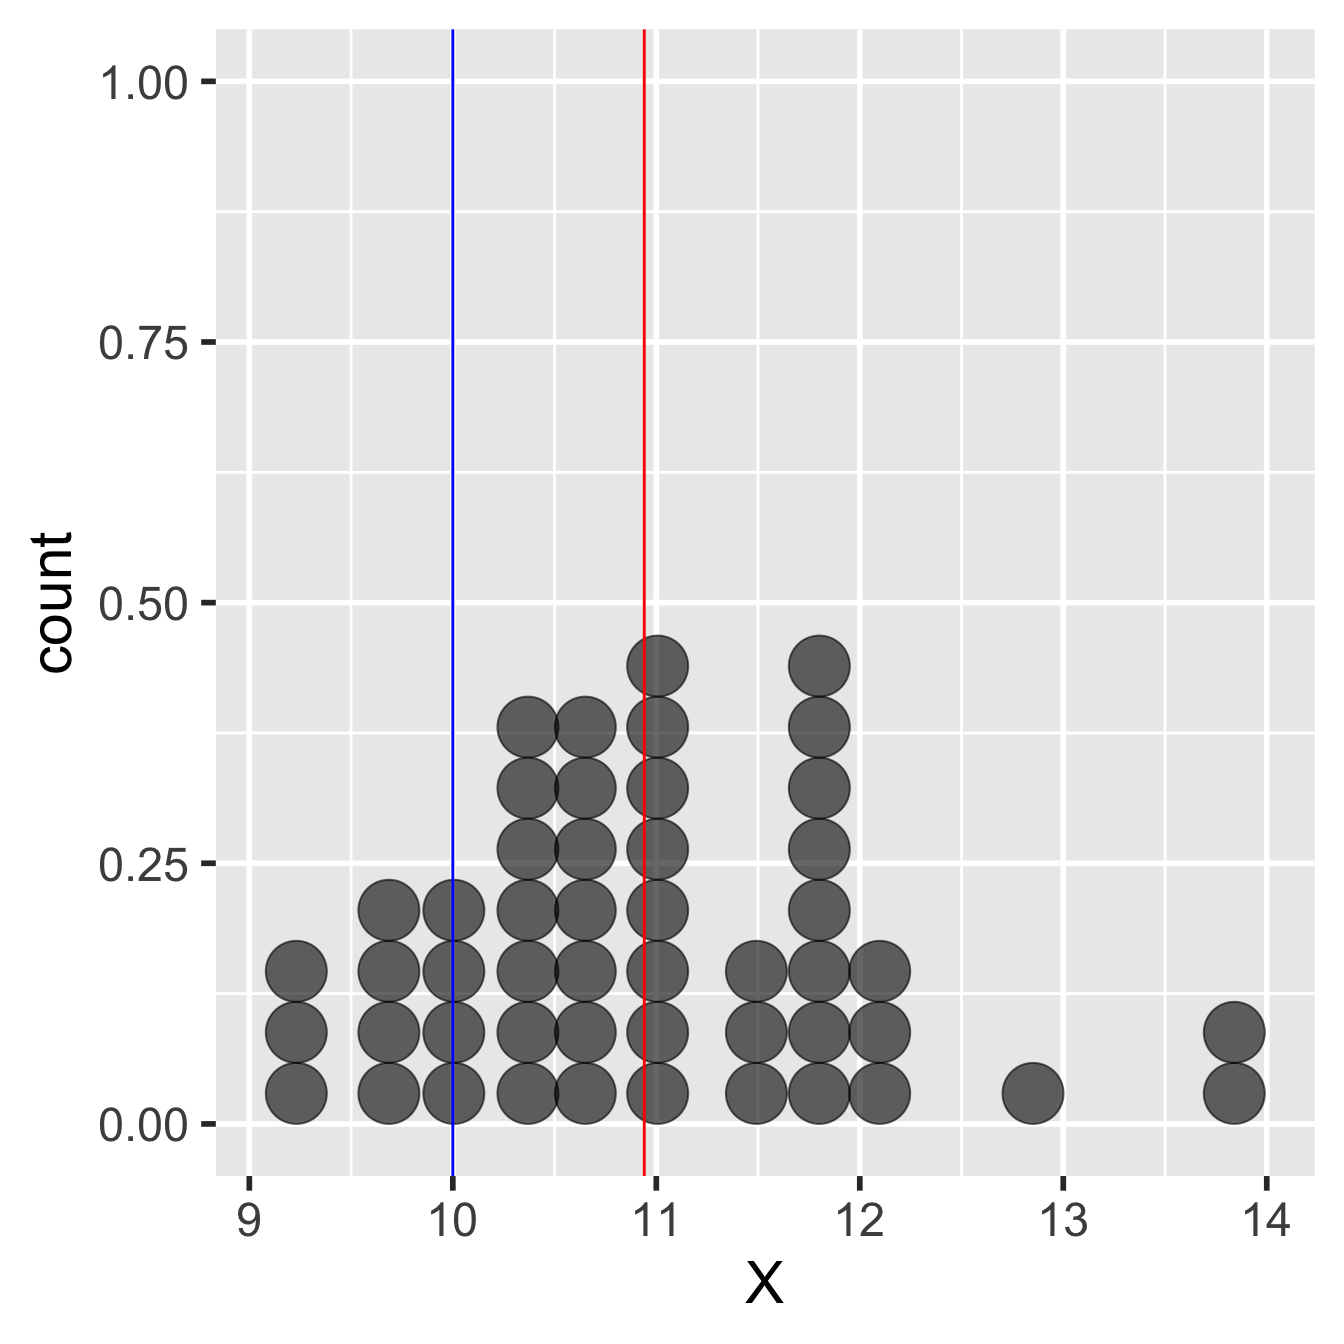
\includegraphics[width=0.55\linewidth]{intro-bio-stats-book_files/figure-latex/one-t-eg-samps-1} 

}

\caption{Example of data used in a one-sample t-test}\label{fig:one-t-eg-samps}
\end{figure}

We're calling the variable `X' in this example. It needs a label, and `X' is as good as any other. The red line shows the sample mean. This is a bit less than 11. The blue line shows the expected value. This is 10, so this example could correspond to the foraging study mentioned above.

The observed sample mean is about one unit larger than the expected value. How do we decide whether the population mean is really different from the expected value? Perhaps the difference between the observed and expected value is due to sampling variation. Here's how a frequentist tackles this kind of question:

\begin{enumerate}
\def\labelenumi{\arabic{enumi}.}
\item
  Set up an appropriate null hypothesis, i.e.~an hypothesis of `no effect' or `no difference'. The null hypothesis in this type of question is that \emph{the population mean is equal to the expected value}.
\item
  Work out what the sampling distribution of a sample mean looks like under the null hypothesis. This is the null distribution. Because we're now using a parametric approach, we will assume this has a particular form.
\item
  Finally, we use the null distribution to assess how likely the observed result is under the null hypothesis. This is the \emph{p}-value calculation that we use to summarise our test.
\end{enumerate}

This chain of reasoning is no different from that developed in the bootstrapping example from earlier. We're just going to make an extra assumption this time to allow us to use a one-sample \emph{t}-test. This extra assumption is that \emph{the variable (`X') is normally distributed in the population}. When we make this normality assumption, the whole process of carrying out the statistical test is actually very simple because the null distribution will have a known mathematical form---it ends up being a \emph{t}-distribution.

We can use this knowledge to construct the test of statistical significance. Instead of using the whole sample, as we did with the bootstrap, now we only need three simple pieces of information to construct the test: the sample size, the sample variance, and the sample mean. The one-sample \emph{t}-test is then carried out as follows:

\textbf{Step 1.} Calculate the sample mean. This happens to be our `best guess' of the unknown population mean. However, its role in the one-sample \emph{t}-test is to allow us to construct a test statistic in the next step.

\textbf{Step 2.} Estimate the standard error of \emph{the sample mean}. This gives us an idea of how much sampling variation we expect to observe. The standard error doesn't depend on the true value of the mean, so the standard error of the sample mean is also the standard error of any mean under any particular null hypothesis.

This second step boils down to applying a simple formula involving the sample size and the standard deviation of the sample:

\[\text{Standard Error of the Mean} = \sqrt{\frac{s^2}{n}}\]

\ldots where \(s^2\) is the square of the standard deviation (the sample variance) and \(n\) is for the sample size. This is the formula introduced in the \protect\hyperlink{parametric-statistics}{parametric statistics} chapter. The standard error of the mean gets smaller as the sample size grows or the sample variance shrinks.

\textbf{Step 3.} Calculate a `test statistic' from the sample mean and standard error. We calculate this by dividing the sample mean (step 1) by its estimated standard error (step 2):

\[\text{t} = \frac{\text{Sample Mean}}{\text{Standard Error of the Mean}}\]

If our normality assumption is reasonable, this test-statistic follows a \emph{t}-distribution. This is guaranteed by the normality assumption. So this particular test statistic is also a \emph{t}-statistic. That's why we label it \emph{t}. This knowledge leads to the final step\ldots{}

\textbf{Step 4.} Compare the \emph{t}-statistic to the theoretical predictions of the \emph{t}-distribution to assess the statistical significance of the difference between observed and expected value. We calculate the probability that we would have observed a difference with a magnitude as large as, or larger than, the observed difference, if the null hypothesis were true. That's the \emph{p}-value for the test.

We could step through the actual calculations involved in these steps in detail, using R to help us, but there's no need to do this. We can let R handle everything for us. But first, we should review the assumptions of the one-sample \emph{t}-test.

\hypertarget{assumptions-of-the-one-sample-t-test}{%
\subsection{\texorpdfstring{Assumptions of the one-sample \emph{t}-test}{Assumptions of the one-sample t-test}}\label{assumptions-of-the-one-sample-t-test}}

Several assumptions need to be met in order for a one-sample~\emph{t}-test to be valid. Some of these are more important than others. We'll start with the most important and work down the list in reverse order of importance:

\begin{enumerate}
\def\labelenumi{\arabic{enumi}.}
\tightlist
\item
  \textbf{Independence.} In rough terms, independence means each observation in the sample does not `depend on' the others. We'll discuss this more carefully when we consider the \protect\hyperlink{experimental-design}{principles of experimental design}. The key thing to know now is why this assumption matters: if the data are not independent, the \emph{p}-values generated by the one-sample \emph{t}-test will be unreliable.
\end{enumerate}

(In fact, the \emph{p}-values will be too small when the non-independence assumption is broken. That means we risk the false conclusion that a difference is statistically significant when in reality, it is not)

\begin{enumerate}
\def\labelenumi{\arabic{enumi}.}
\setcounter{enumi}{1}
\item
  \textbf{Measurement scale.} The variable being analysed should be measured on an interval or ratio scale, i.e.~it should be a numeric variable of some kind. Applying a one-sample~\emph{t}-test to a variable that is not measured on one of these scales doesn't make much sense.
\item
  \textbf{Normality.} The one-sample \emph{t}-test will only produce completely reliable \emph{p}-values when the variable is normally distributed in the population. However, this assumption is less important than many people think. The \emph{t}-test is robust to mild departures from normality when the sample size is small, and when the sample size is large, the normality assumption hardly matters at all.
\end{enumerate}

We don't have the time to explain why the normality assumption is not too important for large samples, but we can at least state the reason: it is a consequence of that central limit theorem we mentioned in the last chapter.

\hypertarget{evaluating-the-assumptions}{%
\subsection{Evaluating the assumptions}\label{evaluating-the-assumptions}}

The first two assumptions---independence and measurement scale---are aspects of experimental design. We can only evaluate these by thinking carefully about how the data were gathered and what was measured. It's too late to do anything about these after we have collected our data.

What about that 3\textsuperscript{rd} assumption---normality? One way to evaluate this is by visualising the sample distribution. For small samples, if the sample distribution looks approximately normal then it's probably fine to use the \emph{t}-test. For large samples, we don't even need to worry about a moderate departure from normality\footnote{It's hard to say what constitutes a `large' sample. If we're lucky enough to be working with hundreds of observations it's fine to ignore mild departures from normality. If we're working with 10s of observations we probably need to pay a bit more attention to the normality assumption in a \emph{t}-test.}.

\hypertarget{carrying-out-a-one-sample-t-test-in-r}{%
\section{\texorpdfstring{Carrying out a one-sample \emph{t}-test in R}{Carrying out a one-sample t-test in R}}\label{carrying-out-a-one-sample-t-test-in-r}}

\begin{infobox}{action}

\hypertarget{section-3}{%
\subsubsection*{}\label{section-3}}
\addcontentsline{toc}{subsubsection}{}

As usual, a good way to understand what follows is by working through the example. Remember, the code again assumes that `MORPH\_DATA.CSV' has been read into a tibble called \texttt{morph\_data}.

\end{infobox}

We'll use the plant morph example again to learn how to carry out a one-sample \emph{t}-test in R. Remember, the data were `collected' to 1) compare the frequency of purple morphs to a prediction and 2) compare the mean dry weight of purple and green morphs. Neither of these questions can be tackled with a one-sample \emph{t}-test.

Instead, let's pretend that we unearthed a report from 30 years ago that found the mean size of purple morphs to be 710 grams. We want to evaluate whether the mean size of purple plants in the contemporary population is different from this expectation, because we think they may have adapted to local conditions.

We only need the purple morph data for this example, so we should first \texttt{filter} the data to get hold of only the purple plants:

\begin{Shaded}
\begin{Highlighting}[]
\CommentTok{\# get just the purple morphs}
\NormalTok{purple\_morphs }\OtherTok{\textless{}{-}} \FunctionTok{filter}\NormalTok{(morph\_data, Colour }\SpecialCharTok{==} \StringTok{"Purple"}\NormalTok{)}
\end{Highlighting}
\end{Shaded}

The \texttt{purple\_morphs} data set has two columns: \texttt{Weight} contains the dry weight biomass of purple plants, and \texttt{Colour} indicates which sample (plant morph) an observation belongs to. We don't need the \texttt{Colour} column anymore because we've just removed all the green plants, but there's no harm in leaving it in.

\hypertarget{visualising-the-data-and-checking-the-assumptions}{%
\subsection{Visualising the data and checking the assumptions}\label{visualising-the-data-and-checking-the-assumptions}}

We start by calculating a few summary statistics and visualising the sample distribution of purple morph dry weights. That's right\ldots{} always check the data before carrying out a statistical analysis! We already looked over these data in the \protect\hyperlink{statistical-comparisons}{Statistical comparisons} chapter. However, we'll proceed as though this is the first time we've seen them to demonstrate a complete workflow.

Here is the \textbf{dplyr} code to produce the descriptive statistics:

\begin{Shaded}
\begin{Highlighting}[]
\NormalTok{purple\_morphs }\SpecialCharTok{\%\textgreater{}\%} 
  \FunctionTok{summarise}\NormalTok{(}\AttributeTok{mean =} \FunctionTok{mean}\NormalTok{(Weight), }
            \AttributeTok{sd =} \FunctionTok{sd}\NormalTok{(Weight),}
            \AttributeTok{samp\_size =} \FunctionTok{n}\NormalTok{())}
\end{Highlighting}
\end{Shaded}

\begin{verbatim}
## # A tibble: 1 x 3
##    mean    sd samp_size
##   <dbl> <dbl>     <int>
## 1  767.  156.        77
\end{verbatim}

We have 77 purple plants in the sample. Not bad but we should keep an eye on the normality assumption. Let's check this by making a histogram with the sample of purple plant dry weights:

\begin{Shaded}
\begin{Highlighting}[]
\FunctionTok{ggplot}\NormalTok{(purple\_morphs, }\FunctionTok{aes}\NormalTok{(}\AttributeTok{x =}\NormalTok{ Weight)) }\SpecialCharTok{+} 
  \FunctionTok{geom\_histogram}\NormalTok{(}\AttributeTok{binwidth =} \DecValTok{50}\NormalTok{)}
\end{Highlighting}
\end{Shaded}

\begin{figure}

{\centering 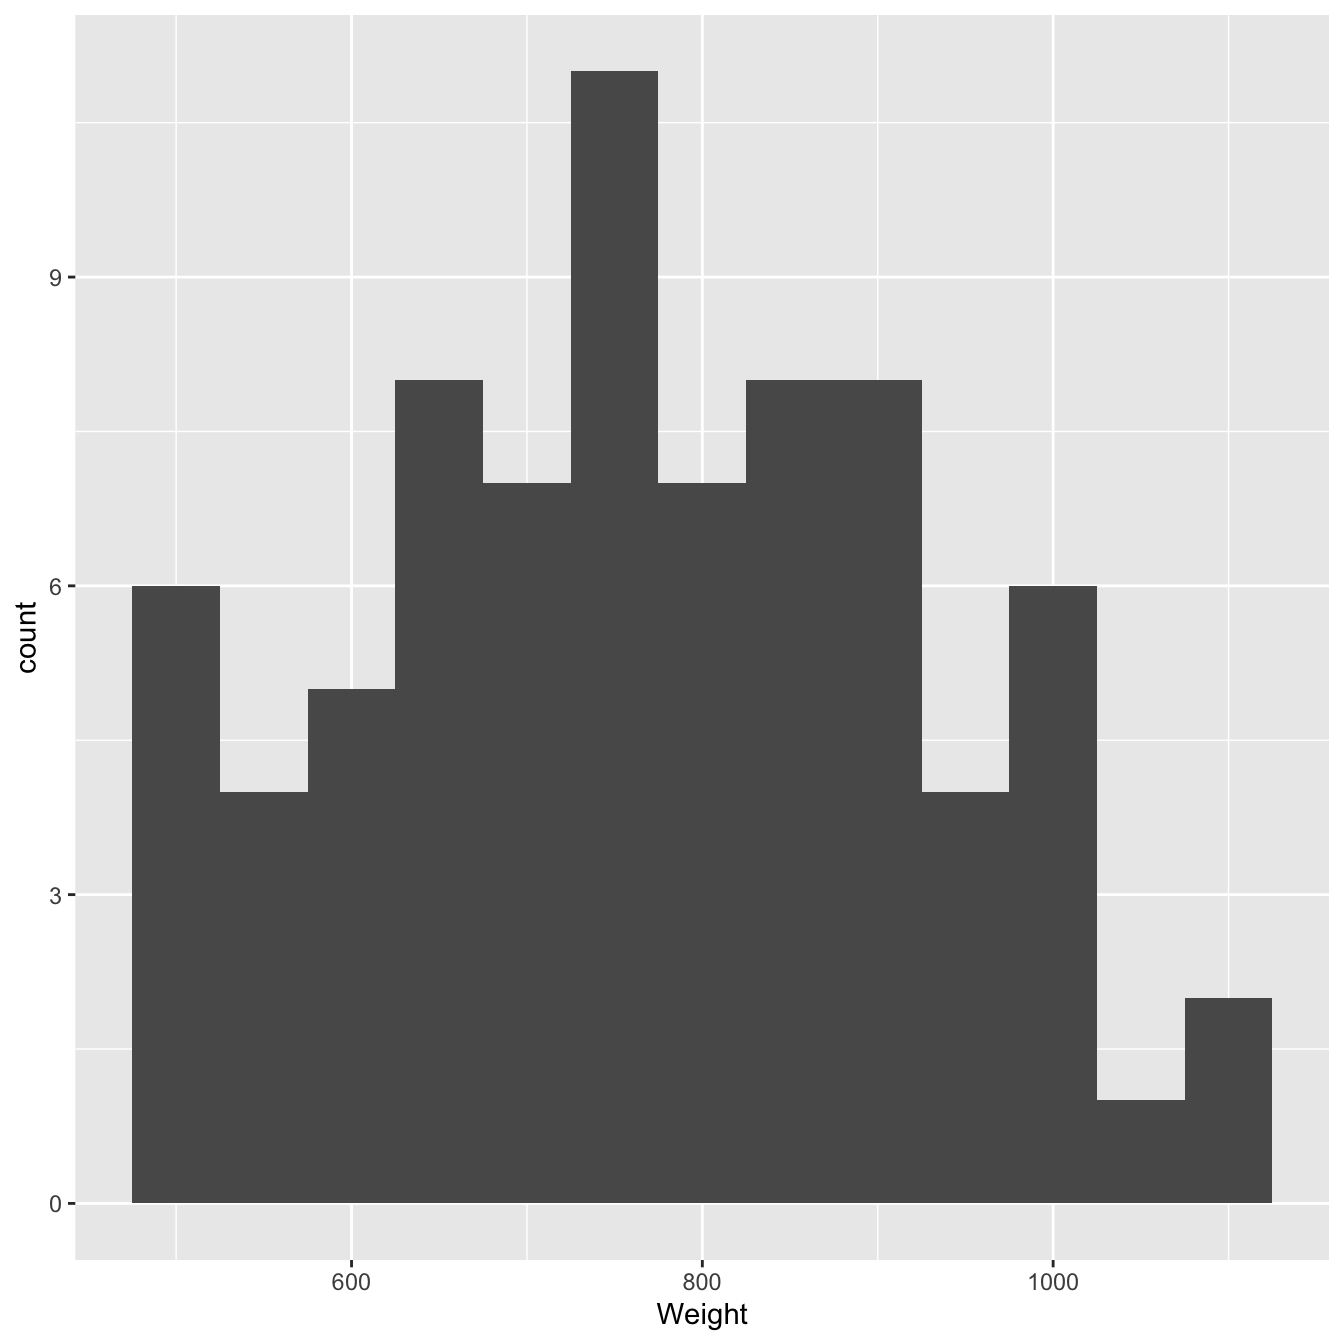
\includegraphics[width=0.6\linewidth]{intro-bio-stats-book_files/figure-latex/purple-morph-dist-again-1} 

}

\caption{Size distributions of purple morph dry weight sample}\label{fig:purple-morph-dist-again}
\end{figure}

These is nothing too `non-normal' about this sample distribution---it's roughly bell-shaped---so it seems reasonable to assume it came from normally distributed population.

\hypertarget{carrying-out-the-test}{%
\subsection{Carrying out the test}\label{carrying-out-the-test}}

It's easy to carry out a one-sample \emph{t}-test in R. We use a function called \texttt{t.test} (no surprises there). Remember, \texttt{Weight} contains the dry weight biomass of purple plants. Here's the R code to carry out a one-sample \emph{t}-test:

\begin{Shaded}
\begin{Highlighting}[]
\FunctionTok{t.test}\NormalTok{(purple\_morphs}\SpecialCharTok{$}\NormalTok{Weight, }\AttributeTok{mu =} \DecValTok{710}\NormalTok{)}
\end{Highlighting}
\end{Shaded}

We have suppressed the output because we initially want to focus on how to use the \texttt{t.test} function. We have to assign two arguments to control what the function does:

\begin{enumerate}
\def\labelenumi{\arabic{enumi}.}
\item
  The first argument (\texttt{purple\_morphs\$Weight}) is simply a numeric vector containing the sample values. Sadly we can't give \texttt{t.test} a data frame when doing a one-sample test. Instead, we have to pull out the column we're interested in using the \texttt{\$} operator.
\item
  The second argument (called \texttt{mu}) sets the expected value to which we want to compare the sample mean. So \texttt{mu\ =\ 710} tells the function to compare the sample mean to a value of 710. This can be any value we like, and the correct value depends on the question we're asking.
\end{enumerate}

That's it for setting up the test. Here is the R code for the test again, this time with the output included:

\begin{Shaded}
\begin{Highlighting}[]
\FunctionTok{t.test}\NormalTok{(purple\_morphs}\SpecialCharTok{$}\NormalTok{Weight, }\AttributeTok{mu =} \DecValTok{710}\NormalTok{)}
\end{Highlighting}
\end{Shaded}

\begin{verbatim}
## 
##  One Sample t-test
## 
## data:  purple_morphs$Weight
## t = 3.1811, df = 76, p-value = 0.002125
## alternative hypothesis: true mean is not equal to 710
## 95 percent confidence interval:
##  731.1490 801.9787
## sample estimates:
## mean of x 
##  766.5638
\end{verbatim}

The first line tells us what kind of \emph{t}-test we used. This says: \texttt{One\ Sample\ t-test}. OK, now we know that we used the one-sample \emph{t}-test (there are other kinds). The next line reminds us about the data. This says: \texttt{data:\ \ purple\_morphs\$Weight}, which is R-speak for 'we compared the mean of the \texttt{Weight} variable to an expected value. Which value? This is given later.

The third line of text is the most important. This says: \texttt{t\ =\ 3.1811,\ df\ =\ 76,\ p-value\ =\ 0.002125}. The first part of this, \texttt{t\ =\ 3.1811}, is the test statistic, i.e.~the value of the \emph{t}-statistic. The second part, \texttt{df\ =\ 76}, summarise the `degrees of freedom'. This is required to work out the \emph{p}-value. It also tells us something about how much `power' our statistical test has (see the box below). The third part, \texttt{p-value\ =\ 0.002125}, is the all-important \emph{p}-value.

That \emph{p}-value indicates a statistically significant difference between the mean dry weight biomass and the expected value of 710 g (\emph{p} is less than 0.05). Because the \emph{p}-value is less than 0.01 but greater than 0.001, we report this as `\emph{p} \textless{} 0.01'. Read through the \protect\hyperlink{presenting-p-values}{Presenting \emph{p}-values} section again if this logic is confusing.

The fourth line of text (\texttt{alternative\ hypothesis:\ true\ mean\ is\ not\ equal\ to\ 710}) tells us the alternative to the null hypothesis (H\textsubscript{1}). More importantly, this reminds us which expected value was used to formulate the null hypothesis (mean = 710).

The next two lines show us the `95\% confidence interval' for the difference between the means. We don't need this information now, but we can think of this interval as a rough summary of the likely values of the `true' mean\footnote{In reality, a frequentist confidence interval is more complicated than that but this book probably isn't the right place to get into that discussion. Take our word for it though---confidence intervals are odd things.}.

The last few lines summarise the sample mean. This might be useful if we had not already calculated.

\begin{infobox}{information}

\hypertarget{a-bit-more-about-degrees-of-freedom}{%
\subsubsection*{A bit more about degrees of freedom}\label{a-bit-more-about-degrees-of-freedom}}
\addcontentsline{toc}{subsubsection}{A bit more about degrees of freedom}

Degrees of freedom (abbreviated d.f. or df) are closely related to the idea of sample size. The greater the degrees of freedom associated with a test, the more likely it is to detect an effect if it's present. To calculate the degrees of freedom, we start with the sample size, and then reduce this number by one for every quantity (e.g.~a mean) we had to calculate to construct the test.

Calculating degrees of freedom for a one-sample \emph{t}-test is easy. The degrees of freedom are just n-1, where n is the number of observations in the sample. We lose one degree of freedom because we have to calculate one sample mean to construct the test.

\end{infobox}

\hypertarget{summarising-the-result}{%
\subsection{Summarising the result}\label{summarising-the-result}}

Having obtained the result, we now need to write our conclusion. We are testing a scientific hypothesis, so we must always return to the original question to write the conclusion. In this case, the appropriate conclusion is:

\begin{quote}
The mean dry weight biomass of purple plants is significantly different from the expectation of 710 grams (\emph{t} = 3.18, d.f. = 76, \emph{p} \textless{} 0.01).
\end{quote}

This is a concise and unambiguous statement in response to our initial question. The statement indicates the result of the statistical test \textbf{and} which value was used in the comparison. It is sometimes appropriate to give the values of the sample mean in the conclusion:

\begin{quote}
The mean dry weight biomass of purple plants (767 grams) is significantly different from the expectation of 710 grams (\emph{t} = 3.18, d.f. = 76, \emph{p} \textless{} 0.01).
\end{quote}

Notice that we include details of the test in the conclusion. However, keep in mind that when writing scientific reports, the reporting of any statistical test should be a conclusion like the one above. \textbf{Simply writing \emph{t} = 3.18 or \emph{p} \textless{} 0.01 is not an adequate.}

There are a number of common questions that arise when presenting \emph{t}-test results:

\begin{enumerate}
\def\labelenumi{\arabic{enumi}.}
\item
  \textbf{What do I do if \emph{t} is negative?} Don't worry. A \emph{t}-statistic can come out negative or positive, it simply depends on which order the two samples are entered into the analysis. Since the absolute value of \emph{t} determines the \emph{p}-value, when presenting the results, just ignore the minus sign and give \emph{t} as a positive number.
\item
  \textbf{How many significant figures for \emph{t}?} The \emph{t}-statistic is conventionally given to 3 significant figures. This is because, in terms of the \emph{p}-value generated, there is almost no difference between, say, \emph{t} = 3.1811 and \emph{t} = 3.18.
\item
  \textbf{Upper or lower case} The \emph{t} statistic should always be written as lower case when writing it in a report (as in the conclusions above). Similarly, d.f. and \emph{p} are always best as lower case. Some statistics we encounter later are written in upper case, but even with these, d.f. and \emph{p} should be lower case.
\item
  \textbf{How should I present \emph{p}?} There are various conventions in use for presenting \emph{p}-values. We discussed these in the \protect\hyperlink{hypotheses-and-p-values}{Hypotheses and \emph{p}-values} chapter. Learn them! It's not possible to understand scientific papers or prepare reports properly without knowing these conventions.
\end{enumerate}

\begin{infobox}{warning}

\hypertarget{p-0.00-its-impossible-p-1e-16-whats-that}{%
\subsubsection*{p = 0.00? It's impossible! p = 1e-16? What's that?}\label{p-0.00-its-impossible-p-1e-16-whats-that}}
\addcontentsline{toc}{subsubsection}{p = 0.00? It's impossible! p = 1e-16? What's that?}

Some statistics packages will sometimes give a probability of \emph{p} = 0.00. This does not mean the probability was really zero. A probability of zero would mean an outcome was impossible, even though it happened! When a computer package reports \emph{p} = 0.00 it just means that the probability was `very small' and ended up being rounded down to 0.

R typically uses a slightly different convention for presenting small probabilities. A very small probability is given as \texttt{p-value\ \textless{}\ 2.2e-16}. What does 2.2e-16 mean? This is R-speak for scientific notation, i.e.~\(2.2e^{-16}\) is equivalent to \(2.2 \times 10^{-16}\).

It is fine to report a result like this as \emph{p} \textless{} 0.001; definitely do not write something like \emph{p} = 2.2e-16.

\end{infobox}

\hypertarget{two-sample-t-test}{%
\chapter{\texorpdfstring{Two-sample \emph{t}-test}{Two-sample t-test}}\label{two-sample-t-test}}

\hypertarget{when-do-we-use-a-two-sample-t-test}{%
\section{\texorpdfstring{When do we use a two-sample \emph{t}-test?}{When do we use a two-sample t-test?}}\label{when-do-we-use-a-two-sample-t-test}}

The two-sample \emph{t}-test is a parametric version of the permutation procedure we studied in the \protect\hyperlink{statistical-comparisons}{statistical comparisons} chapter. The test can be used to compare the means of a numeric variable sampled from two independent populations. A two-sample t-test aims to evaluate whether or not a mean is different in the two populations. Here are two examples:

\begin{itemize}
\item
  We're studying how the dietary habits of Scandinavian eagle-owls vary among seasons. We suspect that the dietary value of a prey item is different in the winter and summer. To evaluate this prediction, we measure the size of Norway rat skulls in the pellets of eagle-owls in summer and winter, and then compare the mean size of rat skulls in each season using a two-sample \emph{t}-test.
\item
  We're interested in the costs of anti-predator behaviour in \emph{Daphnia} spp. We conducted an experiment where we added predator kairomones---chemicals that signal the presence of a predator---to jars containing individual \emph{Daphnia}. There is a second control group where no kairomone was added. The change in body size of individuals was measured after one week. We could use a two-sample \emph{t}-test to compare the mean growth rate in the control and treatment groups.
\end{itemize}

\hypertarget{how-does-the-two-sample-t-test-work}{%
\section{\texorpdfstring{How does the two-sample \emph{t}-test work?}{How does the two-sample t-test work?}}\label{how-does-the-two-sample-t-test-work}}

Imagine we have taken a sample of a variable from two populations, labelled `A' and `B'. We'll call the variable `X' again. Here's an example of how these kinds of data might look if we had a sample of 50 items from each population:

\begin{figure}

{\centering 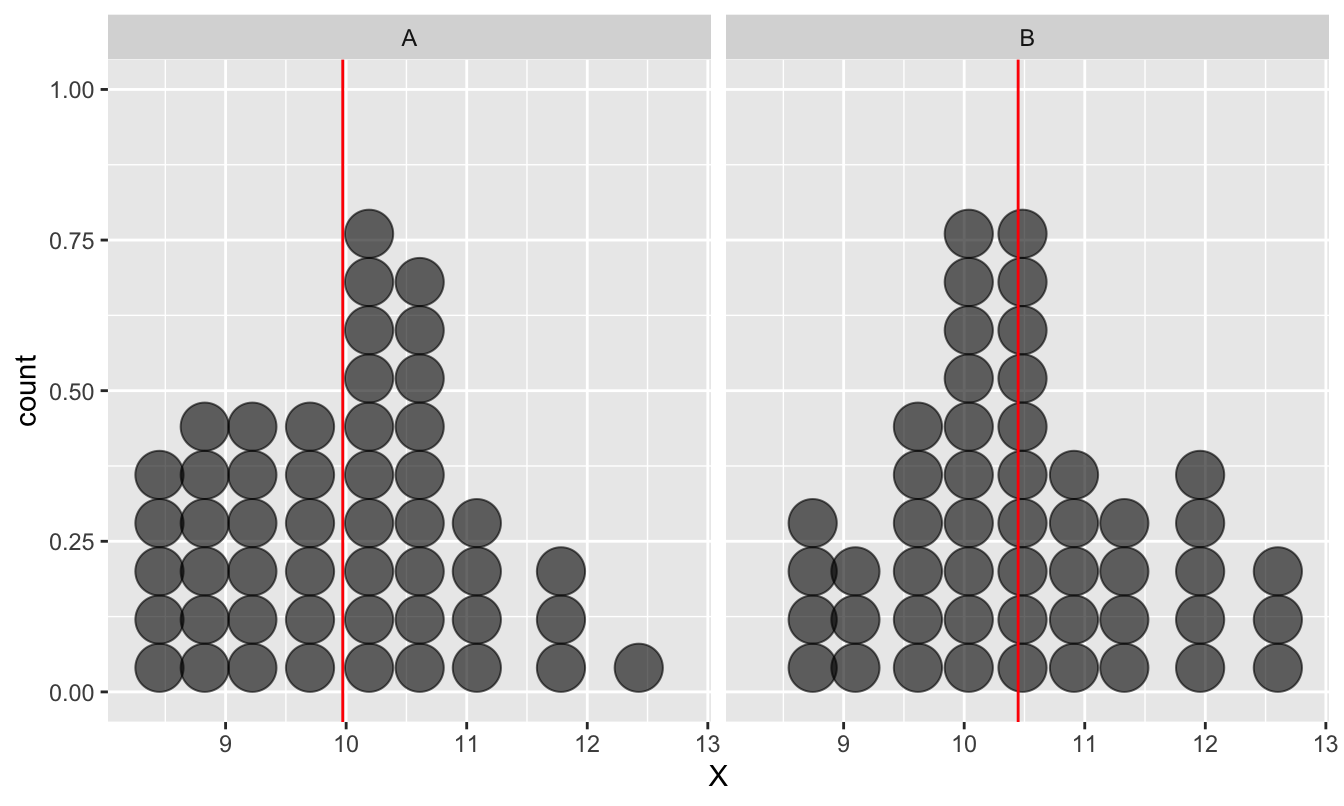
\includegraphics[width=0.8\linewidth]{intro-bio-stats-book_files/figure-latex/two-t-eg-samps-1} 

}

\caption{Example of data used in a two-sample t-test}\label{fig:two-t-eg-samps}
\end{figure}

The first thing to notice is the two distributions overlap quite a lot. However, this observation isn't necessarily all that significant. Why? Because we're not interested in the raw values of `X' in the two samples. It's the \emph{difference between the means} that our test is going to focus on.

The red lines show the mean of each sample. Sample B has a larger mean than sample A. The question is, how do we decide whether this difference is `real', or purely a result of sampling variation?

Using a frequentist approach, we tackle this question by first setting up the appropriate null hypothesis. The null hypothesis here is one of no difference between the population means (they are equal). We then have to work out what the null distribution looks like. This is the sampling distribution of the difference between sample means under the null hypothesis. Once we have the null distribution worked out, we can calculate a \emph{p}-value.

How is this different from the permutation test? The logic is virtually identical. The one key difference is that we have to make an extra assumption to use the two-sample \emph{t}-test. We assume the variable is normally distributed in each population. If this assumption is valid, then the null distribution will have a known form---a \emph{t}-distribution.

We only need a few pieces of information to carry out a two-sample \emph{t}-test. These are basically the same quantities needed to construct the one-sample \emph{t}-test, except now there are two samples involved. We need the sample sizes of groups A and B, the sample variances and the estimated difference between the sample means of X in A and B.

How does a two-sample \emph{t}-test work in practice? It is carried out as follows:

\textbf{Step 1.} Calculate the two sample means, then calculate the difference between these estimates. This estimate is our `best guess' of the true difference between means. As with the one-sample test, its role in the two-sample \emph{t}-test is as a test statistic.

\textbf{Step 2.} Estimate the standard error of \emph{the difference between the sample means} under the null hypothesis of no difference. This gives us an idea of how much sampling variation we expect to observe in the estimated difference if there were actually no difference between the means.

There are a number of different options for estimating this standard error. Each one makes a different assumption about the variability of the two populations. Whatever choice we make, the calculation always boils down to a simple formula involving sample sizes and variances. The standard error gets smaller when the sample sizes grow, or when the sample variances shrink. That's the important point.

\textbf{Step 3.} We can calculate the test statistic once we have estimated the difference between sample means and its standard error. This is a type of \emph{t}-statistic, which we calculate by dividing the difference between sample means (from step 1) by the estimated standard error of the difference (from step 2):

\[\text{t} = \frac{\text{Difference Between Sample Means}}{\text{Standard Error of the Difference}}\]

This \emph{t}-statistic is guaranteed to follow a \emph{t}-distribution if the normality assumption is met. This knowledge leads to the final step\ldots{}

\textbf{Step 4.} Compare the test statistic to the theoretical predictions of the \emph{t}-distribution to assess the statistical significance of the observed difference. That is, we calculate the probability that we would have observed a difference between means with a magnitude as large as, or larger than, the observed difference, if the null hypothesis were true. That's the \emph{p}-value for the test.

We will not step through the various calculations involved in these steps. The formula for the standard two-sample \emph{t}-test and its variants are summarised on the \href{https://en.wikipedia.org/wiki/Student\%27s_t-test\#Independent_two-sample_t-test}{\emph{t}-test Wikipedia page}. There's no need to learn these because we can get R to handle the calculations for us.

Before we do that, we need to review the assumptions of the two-sample \emph{t}-test.

\hypertarget{assumptions-of-the-two-sample-t-test}{%
\subsection{\texorpdfstring{Assumptions of the two-sample \emph{t}-test}{Assumptions of the two-sample t-test}}\label{assumptions-of-the-two-sample-t-test}}

Several assumptions need to be met for a two-sample \emph{t}-test to be valid. These are essentially the same as those for the one-sample version. Starting with the most important and working down in decreasing order of importance, these are:

\begin{enumerate}
\def\labelenumi{\arabic{enumi}.}
\item
  \textbf{Independence.} Remember what we said in our discussion of the one-sample \emph{t}-test? If the data are not independent, the \emph{p}-values generated by the test will be too small, and even mild non-independence can be a serious problem. The same is true of the two-sample \emph{t}-test.
\item
  \textbf{Measurement scale.} The variable we are working with should be measured on an interval or ratio scale, which means it will be numeric. It makes little sense to apply a two-sample \emph{t}-test to a categorical variable of some kind.
\item
  \textbf{Normality.} The two-sample \emph{t}-test will produce reliable \emph{p}-values if the variable is normally distributed in each population. However, the two-sample \emph{t}-test is fairly robust to mild departures from normality and this assumption matters little when the sample sizes are large.
\end{enumerate}

\hypertarget{evaluating-the-assumptions-1}{%
\subsection{Evaluating the assumptions}\label{evaluating-the-assumptions-1}}

How do we evaluate the first two assumptions? As with the one-sample test, these are aspects of experimental design---we can only evaluate them by thinking about the data we've collected.

We can evaluate the normality assumption by plotting the sample distribution \emph{of each group} using, for example, a pair of histograms or dot plots. We must examine the distribution in each group, not the distribution of the combined sample. If both samples looks approximately normal then we can proceed with the test. If we think we can see a departure from normality, we should consider our sample sizes before proceeding. Remember that the test is robust to mild departures when sample sizes are large (e.g.~\textgreater100 observations in each group).

\hypertarget{what-about-the-equal-variance-assumption}{%
\subsection{\texorpdfstring{What about the \emph{equal variance} assumption?}{What about the equal variance assumption?}}\label{what-about-the-equal-variance-assumption}}

It is sometimes said that a two-sample \emph{t}-test requires the variability (`variance') of each sample to be the same, or at least quite similar. This would be true if we used the original version of Student's two-sample \emph{t}-test. However, R doesn't use this version of the test by default. R uses the ``Welch'' two-sample \emph{t}-test. This version of the test does not rely on the equal variance assumption. As long as we stick with this version of the \emph{t}-test, the equal variance assumption isn't something we need to worry about.

\begin{infobox}{information}

\hypertarget{should-we-use-students-original-two-sample-t-test}{%
\subsubsection*{\texorpdfstring{Should we use Student's original two-sample \emph{t}-test?}{Should we use Student's original two-sample t-test?}}\label{should-we-use-students-original-two-sample-t-test}}
\addcontentsline{toc}{subsubsection}{Should we use Student's original two-sample \emph{t}-test?}

The original `equal-variance' two-sample \emph{t}-test is a little more powerful than the Welch version. That is, it is more likely to detect a difference in means (if present). However, the increase in statistical power is really quite small if the sample sizes of each group are similar and the original test is only correct when the population variances are identical. Since we can never prove the `equal variance' assumption---we can only ever reject it---it is generally safer to just use the Welch two-sample \emph{t}-test.

One last warning. Student's two-sample \emph{t}-test assumes the variances of \emph{the populations} are identical. It is the population variances, not the sample variances, that matter. There are methods for comparing variances, and people sometimes suggest using these to select `the right' \emph{t}-test. This is bad advice. For reasons just outlined, there's little advantage to using Student's version of the test if the variances really are the same. What's more, the process of picking the test based on the results of another statistical test affects the reliability of the resulting \emph{p}-values.

\end{infobox}

\hypertarget{carrying-out-a-two-sample-t-test-in-r}{%
\section{\texorpdfstring{Carrying out a two-sample \emph{t}-test in R}{Carrying out a two-sample t-test in R}}\label{carrying-out-a-two-sample-t-test-in-r}}

\begin{infobox}{action}

\hypertarget{section-4}{%
\subsubsection*{}\label{section-4}}
\addcontentsline{toc}{subsubsection}{}

We're going to use the plant morph example one last time. And yes, the code below assumes `MORPH\_DATA.CSV' has been read into a tibble called \texttt{morph\_data}.

\end{infobox}

We'll use the plant morph size example again to learn the workflow for two-sample \emph{t}-tests in R. We'll use the test to evaluate whether or not the mean dry weight of purple plants is different from that of green plants. The background to \emph{why} this comparison is worth doing was covered in the \protect\hyperlink{statistical-comparisons}{statistical comparisons} chapter. We considered this comparison using a permutation test in that chapter. It's much simpler to use a two-sample \emph{t}-test, as we are about to find out\ldots{}

\hypertarget{visualising-the-data-and-checking-the-assumptions-1}{%
\subsection{Visualising the data and checking the assumptions}\label{visualising-the-data-and-checking-the-assumptions-1}}

We start by calculating a few descriptive statistics and visualising the sample distributions of the green and purple morph dry weights. We already did this in the \protect\hyperlink{statistical-comparisons}{statistical comparisons} chapter, but here's the \textbf{dplyr} code for the descriptive statistics again:

\begin{Shaded}
\begin{Highlighting}[]
\NormalTok{morph\_data }\SpecialCharTok{\%\textgreater{}\%} 
  \CommentTok{\# group the data by plant morph}
  \FunctionTok{group\_by}\NormalTok{(Colour) }\SpecialCharTok{\%\textgreater{}\%} 
  \CommentTok{\# calculate the mean, standard deviation and sample size}
  \FunctionTok{summarise}\NormalTok{(}\AttributeTok{mean =} \FunctionTok{mean}\NormalTok{(Weight), }
            \AttributeTok{sd =} \FunctionTok{sd}\NormalTok{(Weight),}
            \AttributeTok{samp\_size =} \FunctionTok{n}\NormalTok{())}
\end{Highlighting}
\end{Shaded}

\begin{verbatim}
## # A tibble: 2 x 4
##   Colour  mean    sd samp_size
##   <chr>  <dbl> <dbl>     <int>
## 1 Green   708.  150.       173
## 2 Purple  767.  156.        77
\end{verbatim}

As we already know, the purple plants tend to be bigger than green plants. The sample sizes are 173 (green plants) and 77 (purple plants). These are good-sized samples, which means we probably don't need to be too obsessed with the normality assumption. However, we still need to visualise the sample distributions to be sure they aren't too odd or contain obvious outliers:

\begin{Shaded}
\begin{Highlighting}[]
\FunctionTok{ggplot}\NormalTok{(morph\_data, }\FunctionTok{aes}\NormalTok{(}\AttributeTok{x =}\NormalTok{ Weight)) }\SpecialCharTok{+} 
  \FunctionTok{geom\_histogram}\NormalTok{(}\AttributeTok{binwidth =} \DecValTok{50}\NormalTok{) }\SpecialCharTok{+} 
  \FunctionTok{facet\_wrap}\NormalTok{(}\SpecialCharTok{\textasciitilde{}}\NormalTok{Colour, }\AttributeTok{ncol =} \DecValTok{1}\NormalTok{)}
\end{Highlighting}
\end{Shaded}

\begin{figure}

{\centering 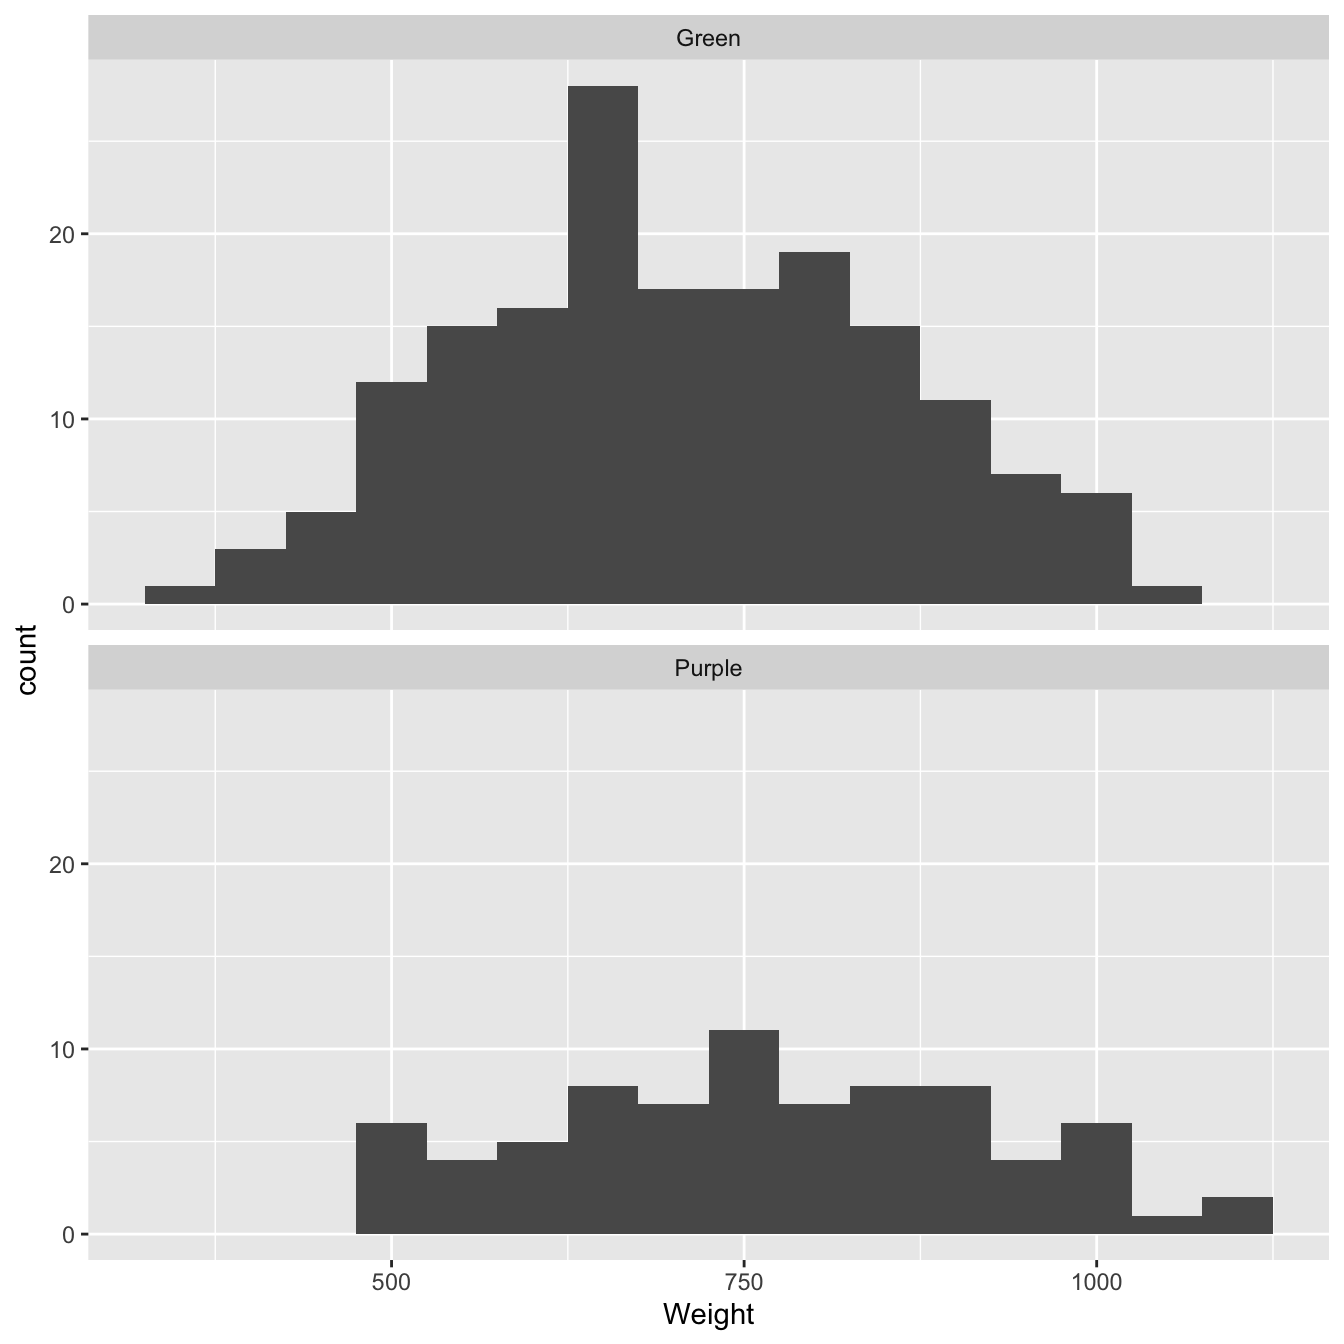
\includegraphics[width=0.6\linewidth]{intro-bio-stats-book_files/figure-latex/two-morph-dist-again-1} 

}

\caption{Size distributions of purple and green morph samples}\label{fig:two-morph-dist-again}
\end{figure}

There is nothing too `non-normal' about the two samples in this example, so it's reasonable to assume they both came from normally distributed populations.

\hypertarget{carrying-out-the-test-1}{%
\subsection{Carrying out the test}\label{carrying-out-the-test-1}}

The function we need to carry out a two-sample \emph{t}-test in R is the \texttt{t.test} function, i.e.~the same functions used for the one-sample test.

Remember, \texttt{morph\_data} has two columns: \texttt{Weight} contains the dry weight biomass of each plant, and \texttt{Colour} is an index variable that indicates which sample (plant morph) an observation belongs to. Here's the code to carry out the two-sample \emph{t}-test:

\begin{Shaded}
\begin{Highlighting}[]
\FunctionTok{t.test}\NormalTok{(Weight }\SpecialCharTok{\textasciitilde{}}\NormalTok{ Colour,  morph\_data)}
\end{Highlighting}
\end{Shaded}

We suppressed the output, for now, to focus on how to use the function. We have to assign two arguments:

\begin{enumerate}
\def\labelenumi{\arabic{enumi}.}
\item
  The first argument is something called a \textbf{formula}. We know this because it includes a `tilde' symbol: \texttt{\textasciitilde{}}. The variable name on the left of the \texttt{\textasciitilde{}} must be the variable whose mean we want to compare (\texttt{Weight}). The variable on the right must be the indicator variable that says which group each observation belongs to (\texttt{Colour}).
\item
  The second argument is the name of the data frame that contains the variables listed in the formula.
\end{enumerate}

Let's take a look at the output:

\begin{Shaded}
\begin{Highlighting}[]
\FunctionTok{t.test}\NormalTok{(Weight }\SpecialCharTok{\textasciitilde{}}\NormalTok{ Colour,  morph\_data)}
\end{Highlighting}
\end{Shaded}

\begin{verbatim}
## 
##  Welch Two Sample t-test
## 
## data:  Weight by Colour
## t = -2.7808, df = 140.69, p-value = 0.006165
## alternative hypothesis: true difference in means between group Green and group Purple is not equal to 0
## 95 percent confidence interval:
##  -100.46812  -16.97476
## sample estimates:
##  mean in group Green mean in group Purple 
##             707.8424             766.5638
\end{verbatim}

The first line reminds us what kind of \emph{t}-test we used. This says: \texttt{Welch\ two-sample\ t-test}, so we know that we used the Welch version of the test that accounts for the possibility of unequal variance. The next line reminds us about the data. This says: \texttt{data:\ Weight\ by\ Colour}, which is R-speak for `we compared the means of the \texttt{Weight} variable, where the group membership is defined by the values of the \texttt{Colour} variable'.

The third line of text is the most important. This says: \texttt{t\ =\ -2.7808,\ d.f.\ =\ 140.69,\ p-value\ =\ 0.006165}. The first part, \texttt{t\ =\ -2.7808}, is the test statistic (i.e.~the value of the \emph{t}-statistic). The second part, \texttt{df\ =\ 140.69}, summarise the `degrees of freedom' (see the box below). The third part, \texttt{p-value\ =\ 0.006165}, is the all-important p-value. This says there is a statistically significant difference in the mean dry weight biomass of the two colour morphs, because \emph{p}\textless0.05. Because the \emph{p}-value is less than 0.01 but greater than 0.001, we would report this as `\emph{p} \textless{} 0.01'.

The fourth line of text (\texttt{alternative\ hypothesis:\ true\ difference\ in\ means\ is\ not\ equal\ to\ 0}) reminds us of the alternative to the null hypothesis (H\textsubscript{1}). This isn't hugely important or interesting.

The next two lines show us the `95\% confidence interval' for the difference between the means. Just as with the one-sample \emph{t}-test we can think of this interval as a rough summary of the likely values of the true difference (again, a confidence interval is more complicated than that in reality).

The last few lines summarise the sample means of each group. This could be useful if we did not bother to calculate these already.

\begin{infobox}{information}

\hypertarget{a-bit-more-about-degrees-of-freedom-1}{%
\subsubsection*{A bit more about degrees of freedom}\label{a-bit-more-about-degrees-of-freedom-1}}
\addcontentsline{toc}{subsubsection}{A bit more about degrees of freedom}

In the original version of the two-sample \emph{t}-test (the one that assumes equal variances), the degrees of freedom of the test are given by (n\textsubscript{A}-1) + (n\textsubscript{B}-1), where n\textsubscript{A} is the number of observations in sample A, and n\textsubscript{B} the number of observations in sample B. The plant morph data included 77 purple plants and 173 green plants, so if we had used the original version of the test we would have (77-1) + (173-1) = 248 d.f.

The Welch version of the \emph{t}-test reduces the degrees of freedom by using a formula that takes into account the difference in variance in the two samples. The greater the difference in the two sample sizes, the smaller the number of degrees of freedom becomes:

\begin{itemize}
\item
  When the sample sizes are similar, the adjusted d.f. will be close to that in the original version of the two-sample \emph{t}-test.
\item
  When the sample sizes are very different, the adjusted d.f. will be close to the sample size of the smallest sample.
\end{itemize}

Notice that the `unequal sample size accounting' results in degrees of freedom that are not whole numbers.

We don't need to know all of this to use the test. Here's the important point: whatever flavour of \emph{t}-test we're using, a test with high degrees of freedom is more powerful than one with low degrees of freedom, i.e.~the higher the degrees of freedom, the more likely we are to detect an effect if it is present. This is why degrees of freedom matter.

\end{infobox}

\hypertarget{summarising-the-result-1}{%
\subsection{Summarising the result}\label{summarising-the-result-1}}

Having obtained the result, we need to report it. We should go back to the original question to do this. In our example, the appropriate summary is:

\begin{quote}
Mean dry weight biomass of purple and green plants differs significantly (Welch's t = 2.78, d.f. = 140.7, \emph{p} \textless{} 0.01), with purple plants being the larger.
\end{quote}

This is a concise and unambiguous statement in response to our initial question. The statement indicates the result of the statistical test \textbf{and} which of the mean values is the larger (readers usually want to know this). Alternatively, we might prefer to give the values of the two means:

\begin{quote}
The mean dry weight biomass of purple plants (767 grams) is significantly greater than that of green plants (708 grams) (Welch's \emph{t} = 2.78, d.f. = 140.7, \emph{p} \textless{} 0.01)
\end{quote}

When writing scientific reports, the result of any statistical test should be a statement like the one above---simply writing t = 2.78 or p \textless{} 0.01 is not an adequate conclusion!

\hypertarget{part-correlation-and-regression}{%
\part{Correlation and Regression}\label{part-correlation-and-regression}}

\hypertarget{correlation-tests}{%
\chapter{Correlation tests}\label{correlation-tests}}

We're going to consider `correlation' in this chapter. A correlation is a statistical measure of \textbf{association} between two variables. An association is any relationship between the variables that makes them dependent in some way: knowing the value of one variable gives you information about the possible values of the other.

The terms `association' and `correlation' are often used interchangeably but strictly speaking, correlation has a narrower definition. Correlation analysis quantifies the degree to which an association tends to a certain pattern via a measure called a \textbf{correlation coefficient}. For example, the correlation coefficient studied below---Pearson's correlation coefficient---measures the degree to which two variables tend toward a straight line relationship.

There are different methods for quantifying correlation, but these all share a number of properties:

\begin{enumerate}
\def\labelenumi{\arabic{enumi}.}
\tightlist
\item
  If there is no relationship between the variables, the correlation coefficient will be zero. The closer to 0 the value, the weaker the relationship. A perfect correlation will be either -1 or +1, depending on the direction. This is illustrated in the figure below:
\end{enumerate}

\begin{center}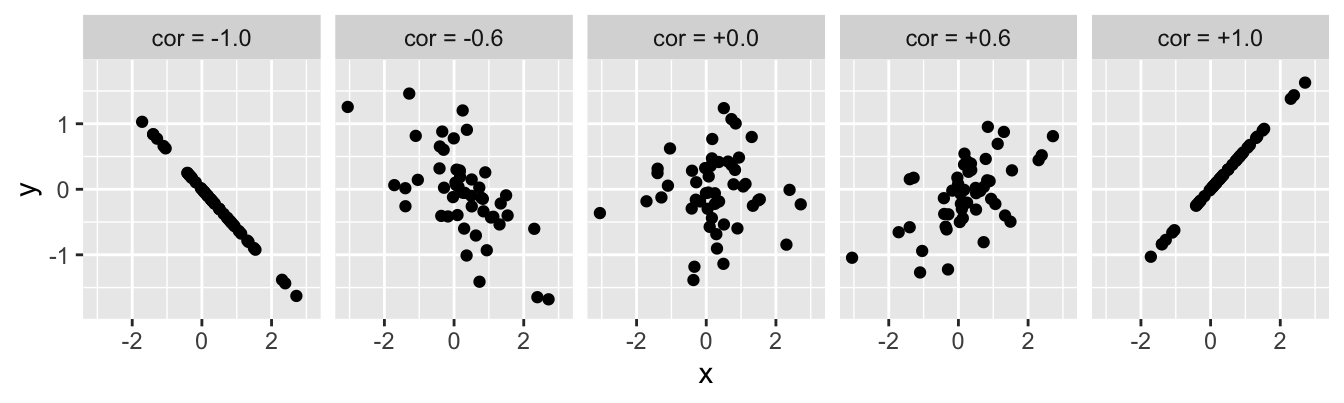
\includegraphics[width=0.8\linewidth]{intro-bio-stats-book_files/figure-latex/cor-strength-eg-1} \end{center}

\begin{enumerate}
\def\labelenumi{\arabic{enumi}.}
\setcounter{enumi}{1}
\item
  The value of a correlation coefficient indicates the direction and strength of the association, but it says nothing about the steepness of the relationship. A correlation coefficient is just a number, so it can't tell us exactly how one variable depends on the other.
\item
  Correlation coefficients do not describe `directional' or `casual' relationships. We can't use correlations to make predictions about one variable based on knowledge of another or make statements about the effect of one variable on the other.
\item
  A correlation coefficient doesn't tell us whether an association is likely to be `real' or not. We have to use a statistical significance test to evaluate whether a correlation may be different from zero. Like any statistical test, this requires certain assumptions about the variables to be met.
\end{enumerate}

We're going to make sense of all this by studying one particular correlation coefficient in this chapter: \textbf{Pearson's product-moment correlation coefficient} (\(r\)). Various measures of association exist, so why focus on this one? Well\ldots{} once you know how to work with one type of correlation in R, it isn't hard to use another. Pearson's product-moment correlation coefficient is the most well-known, which means it is as good a place as any to learn about correlation analysis.

\hypertarget{pearsons-product-moment-correlation}{%
\section{Pearson's product-moment correlation}\label{pearsons-product-moment-correlation}}

What do we need to know about Pearson's product-moment correlation? Let's start with the naming conventions. People often use ``Pearson's correlation coefficient'' or ``Pearson's correlation'' as a convenient shorthand because writing ``Pearson's product-moment correlation coefficient'' all the time soon becomes tedious. If we want to be concise, we can use the standard mathematical symbol to denote Pearson's correlation coefficient---lower case `\(r\)'.

The one thing we absolutely have to know about Pearson's correlation coefficient is that it is \textbf{a measure of linear association between numeric variables}. This means Pearson's correlation is appropriate when numeric variables follow a `straight-line' relationship. That doesn't mean they have to be perfectly related, by the way. It simply means there shouldn't be any `curviness' to their pattern of association\footnote{If non-linear associations \emph{are} apparent it's generally better to use a different correlation coefficient (we'll consider one alternative later in the book).}.

Finally, calculating Pearson's correlation coefficient serves to \emph{estimate} the strength of an association. An estimate can't tell us whether that association is likely to be `real' or not. We need a statistical test to tackle that question. There is a standard parametric test associated with Pearson's correlation coefficient. Unfortunately, this does not have its own name. We will call it ``Pearson's correlation test'' to distinguish the test from the coefficient. Just keep in mind these are not `official' names.

\hypertarget{pearsons-correlation-test}{%
\subsection{Pearson's correlation test}\label{pearsons-correlation-test}}

The logic underpinning Pearson's correlation test is the same as we've seen in previous tests:

\begin{enumerate}
\def\labelenumi{\arabic{enumi}.}
\tightlist
\item
  Define a null hypothesis.
\item
  Calculate an appropriate test statistic.
\item
  Work out the null distribution of that statistic.
\item
  Use this to calculate a~\emph{p}-value from the observed coefficient.
\end{enumerate}

We won't work through the details other than to note a few important aspects:

\begin{itemize}
\tightlist
\item
  When working with Pearson's correlation coefficient, the `no effect' null hypothesis corresponds to one of zero (linear) association between the two variables (\(r=0\)).
\item
  The test statistic associated with \(r\) turns out to be a \emph{t}-statistic. This has nothing to do with comparing means---\emph{t}-statistics pop up all the time in frequentist statistics.
\end{itemize}

Like any parametric technique, Pearson's correlation test makes several assumptions. These need to be met in order for the statistical test to be reliable. The assumptions are:

\begin{itemize}
\tightlist
\item
  Both variables are measured on an interval or ratio scale.
\item
  The two variables are normally distributed (in the population).
\item
  The relationship between the variables is linear.
\end{itemize}

The first two requirements should not need any further explanation at this point---we've seen them before in the context of the one- and two-sample \emph{t}-tests. The third one stems from Pearson's correlation coefficient being a measure of linear association.

Only the linearity assumption needs to be met for Pearson's correlation coefficient (\(r\)) to be a valid measure of association. As long as the relationship between two variables is linear, \(r\) produces a sensible measure of association. However, the first two assumptions need to be met for the associated statistical test to be appropriate.

That's enough background and abstract concepts. Let's see how to perform correlation analysis in R using Pearson's correlation coefficient.

\hypertarget{pearsons-product-moment-correlation-coefficient-in-r}{%
\section{Pearson's product-moment correlation coefficient in R}\label{pearsons-product-moment-correlation-coefficient-in-r}}

\begin{infobox}{action}

\hypertarget{section-5}{%
\subsubsection*{}\label{section-5}}
\addcontentsline{toc}{subsubsection}{}

We will use a new data set to demonstrate correlation analysis. The data live in a file called `BRACKEN.CSV'. The code below assumes those data have been read into a tibble called \texttt{bracken}. Set that up if you plan to work along.

\end{infobox}

The plant morph example is not suitable for correlation analysis. We need a new example to motivate a workflow for correlation tests in R. The example we're going use is about the association between ferns and heather\ldots{}

Bracken fern (\emph{Pteridium aquilinum}) is a common plant in many upland areas. A land manager needs to know whether there is any association between bracken and heather (\emph{Calluna vulgaris}) in these areas. To determine whether the two species are associated, she sampled 22 plots at random and estimated the density of bracken and heather in each plot. The data are the mean \emph{Calluna} standing crop (g m\textsuperscript{-2}) and the number of bracken fronds per m\textsuperscript{2}.

\hypertarget{visualising-the-data-and-checking-the-assumptions-2}{%
\subsection{Visualising the data and checking the assumptions}\label{visualising-the-data-and-checking-the-assumptions-2}}

We can start by printing some information about the \texttt{bracken} data:

\begin{Shaded}
\begin{Highlighting}[]
\FunctionTok{glimpse}\NormalTok{(bracken)}
\end{Highlighting}
\end{Shaded}

\begin{verbatim}
## Rows: 22
## Columns: 2
## $ Calluna <dbl> 980, 760, 613, 489, 498, 416, 589, 510, 459, 680, 471, 145, 25~
## $ Bracken <dbl> 2.3, 1.4, 4.0, 3.6, 4.3, 4.0, 6.3, 6.5, 8.3, 8.2, 8.1, 9.1, 8.~
\end{verbatim}

There are 22 observations (rows) and two variables (columns) in this data set. The two variables, \texttt{Calluna} and \texttt{Bracken}, contain the estimates of heather and bracken abundance in each plot, respectively.

We should always explore the data thoroughly before carrying out any kind of statistical analysis. To begin, we can visualise the form of the association with a scatter plot:

\begin{Shaded}
\begin{Highlighting}[]
\FunctionTok{ggplot}\NormalTok{(bracken, }\FunctionTok{aes}\NormalTok{(}\AttributeTok{x =}\NormalTok{ Calluna, }\AttributeTok{y =}\NormalTok{ Bracken)) }\SpecialCharTok{+}
  \FunctionTok{geom\_point}\NormalTok{()}
\end{Highlighting}
\end{Shaded}

\begin{center}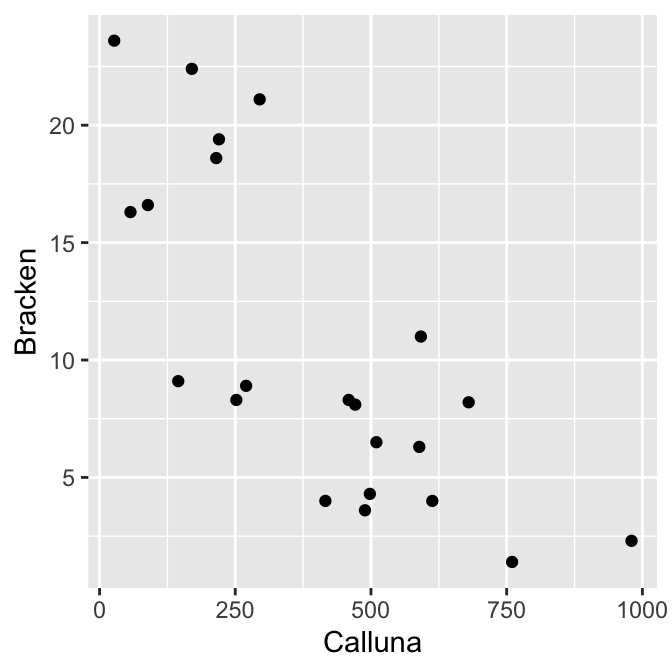
\includegraphics{intro-bio-stats-book_files/figure-latex/bracken-calluna-scatter-1} \end{center}

There appears to be a strong negative association between the species' abundances, and the relationship seems to follow a `straight line' pattern. It looks like Pearson's correlation is a reasonable measure of association for these data.

We will confirm this with a significance test. Is it appropriate to carry out the test? We're dealing with numeric variables measured in ratio scale (assumption 1). What about their distributions (assumptions 2)? Here's a quick visual summary:

\begin{Shaded}
\begin{Highlighting}[]
\FunctionTok{ggplot}\NormalTok{(bracken, }\FunctionTok{aes}\NormalTok{(}\AttributeTok{x =}\NormalTok{ Calluna)) }\SpecialCharTok{+} \FunctionTok{geom\_dotplot}\NormalTok{(}\AttributeTok{binwidth =} \DecValTok{100}\NormalTok{)}
\FunctionTok{ggplot}\NormalTok{(bracken, }\FunctionTok{aes}\NormalTok{(}\AttributeTok{x =}\NormalTok{ Bracken)) }\SpecialCharTok{+} \FunctionTok{geom\_dotplot}\NormalTok{(}\AttributeTok{binwidth =} \DecValTok{2}\NormalTok{)}
\end{Highlighting}
\end{Shaded}

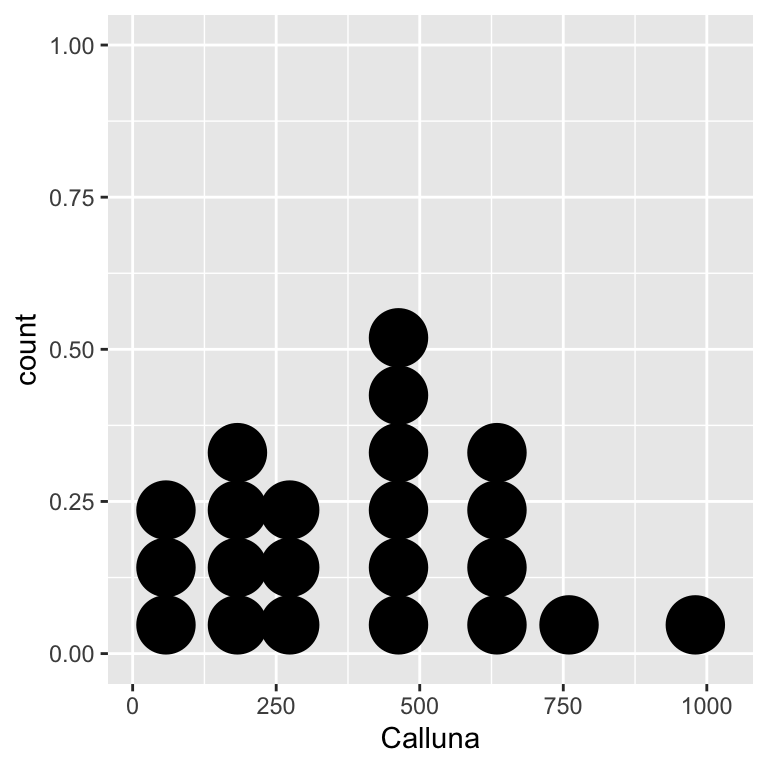
\includegraphics[width=0.4\linewidth]{intro-bio-stats-book_files/figure-latex/bracken-calluna-dist-1} 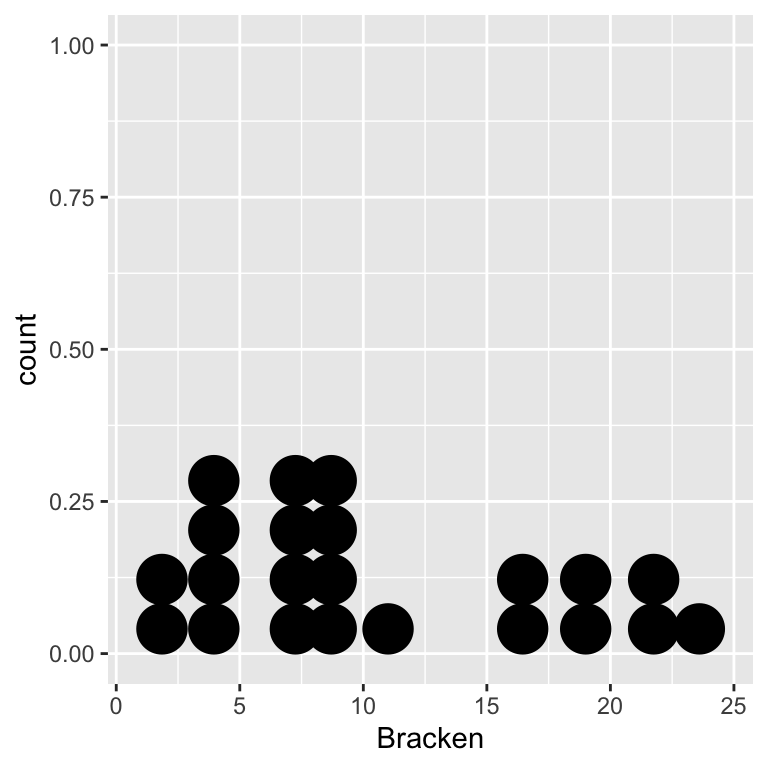
\includegraphics[width=0.4\linewidth]{intro-bio-stats-book_files/figure-latex/bracken-calluna-dist-2}

These dot plots suggest the normality assumption is met, i.e.~both distributions are roughly `bell-shaped'.

That's all three assumptions met---the variables are on a ratio scale, dot the normality assumption is met, and the abundance relationship is linear. It looks like the statistical test will give reliable results.

\hypertarget{doing-the-test}{%
\subsection{Doing the test}\label{doing-the-test}}

Let's proceed with the analysis\ldots{} Carrying out a correlation analysis in R is straightforward. We use the \texttt{cor.test} function to do this:

\begin{Shaded}
\begin{Highlighting}[]
\FunctionTok{cor.test}\NormalTok{(}\SpecialCharTok{\textasciitilde{}}\NormalTok{ Calluna }\SpecialCharTok{+}\NormalTok{ Bracken, }\AttributeTok{method =} \StringTok{"pearson"}\NormalTok{, }\AttributeTok{data =}\NormalTok{ bracken)}
\end{Highlighting}
\end{Shaded}

We have suppressed the output here to focus on how the function works:

\begin{itemize}
\item
  We use the R formula syntax to determine which pair of variables are analysed. The \texttt{cor.test} function expects the two variable names to appear to the right of the \texttt{\textasciitilde{}}, separated by a \texttt{+} symbol, with nothing on the left.
\item
  We use \texttt{method\ =\ "pearson"} to control which type of correlation coefficient was calculated. The default method is Pearson's correlation, but it never hurts to be explicit, so we wrote \texttt{method\ =\ "pearson"} anyway.
\item
  When we use the formula syntax, as we are doing here, we have to tell the function where to find the variables. That's the \texttt{data\ =\ bracken} part.
\end{itemize}

Notice \texttt{cor.test} uses a different convention from the \texttt{t.test} function for the formula argument of. \texttt{t.test} places one variable on the left and the other variable on the right-hand side of the \texttt{\textasciitilde{}} (e.g.~\texttt{Calluna\ \textasciitilde{}\ Bracken}), whereas \texttt{cor.test} requires both two variables to appear to the right of the \texttt{\textasciitilde{}}, separated by a \texttt{+} symbol. This convention exists to emphasise the absence of `directionality' in correlations, i.e.~neither variable has a special status. This will probably make more sense after covering `regression' in later chapters.

The output from the \texttt{cor.test} is, however, very similar to that produced by the \texttt{t.test} function. Here it is:

\begin{verbatim}
## 
##  Pearson's product-moment correlation
## 
## data:  Calluna and Bracken
## t = -5.2706, df = 20, p-value = 3.701e-05
## alternative hypothesis: true correlation is not equal to 0
## 95 percent confidence interval:
##  -0.8960509 -0.5024069
## sample estimates:
##        cor 
## -0.7625028
\end{verbatim}

We won't step through most of this as its meaning should be clear. The \texttt{t\ =\ -5.2706,\ df\ =\ 20,\ p-value\ =\ 3.701e-05} line is the one we really care about:

\begin{itemize}
\tightlist
\item
  The first part says that the test statistic associated with the test is a \emph{t}-statistic, where \texttt{t\ =\ -5.27}. Remember, this has nothing to do with `comparing means'.
\item
  Next, we see the degrees of freedom for the test. Can you see where this comes from? It is \(n-2\), where \(n\) is the sample size. Together, the degrees of freedom and the \emph{t}-statistic determine the \emph{p}-value.
\item
  The \emph{t}-statistic and associated \emph{p}-value are generated under the null hypothesis of zero correlation (\(r = 0\)). Since \emph{p} \textless{} 0.05, we conclude that there is a statistically significant correlation between bracken and heather.
\end{itemize}

What is the actual correlation between bracken and heather densities? That's given at the bottom of the test output: \(-0.76\). As expected from the scatter plot, there is quite a strong negative association between bracken and heather densities.

\hypertarget{reporting-the-result}{%
\subsection{Reporting the result}\label{reporting-the-result}}

When using Pearson's method, we should report the value of the correlation coefficient, the sample size, and the \emph{p}-value\footnote{People occasionally report the value of the correlation coefficient, the \emph{t}-statistic, the degrees of freedom, and the \emph{p}-value. We won't do this.}. Here's how to report the results of this analysis:

\begin{quote}
There is a negative correlation between bracken and heather among the study plots (r=-0.76, n=22, p \textless{} 0.001).
\end{quote}

Notice that we stated the direction of the association. After all, that's what matters to the land manager.

\hypertarget{next-steps}{%
\section{Next steps}\label{next-steps}}

When we summarised the result, we did not say that bracken is having a negative \emph{effect} on the heather, or \emph{vice versa}. It might well be true that bracken has a negative effect on heather. However, our correlation analysis only characterises the association between bracken and heather\footnote{There is a second subtler limitation to this analysis: it was conducted using data from an observational study. If we want to say something about how bracken \emph{affects} heather then we have to conduct an experimental manipulation (e.g.~removing bracken from some plots).}. If we want to make statements about one species is related to the other, we need use a different kind of analysis. That's the focus of our next topic: simple linear regression.

\hypertarget{relationships-and-regression}{%
\chapter{Relationships and regression}\label{relationships-and-regression}}

\hypertarget{introduction-1}{%
\section{Introduction}\label{introduction-1}}

Much of biology is concerned with relationships between numeric variables. For example:

\begin{itemize}
\tightlist
\item
  We sample fish and measure their length and weight because we want to understand how weight changes with length.
\item
  We survey grassland plots and measure soil pH and species diversity to understand how species diversity depends on soil pH.
\item
  We manipulate temperature and measure fitness in insects because we want to describe their thermal tolerance.
\end{itemize}

In the previous chapter, we learnt about one technique for analysing associations between numeric variables (correlation). A correlation coefficient quantifies the strength and direction of an association between two variables: it will be close to zero if there is no association between the variables, whereas a strong association is implied if the coefficient is near -1 or +1. A correlation coefficient tells us nothing about the form of a relationship. Nor does it allow us to predict the value of one variable from the value of a second variable.

In contrast to correlation, a regression analysis allows us to make precise statements about how one numeric variable depends on the values of another. Graphically, we can evaluate such dependencies using a scatter plot. We may be interested in knowing:

\begin{enumerate}
\def\labelenumi{\arabic{enumi}.}
\tightlist
\item
  Are the variables related or not? There's not much point in studying a relationship that isn't there:
\end{enumerate}

\begin{center}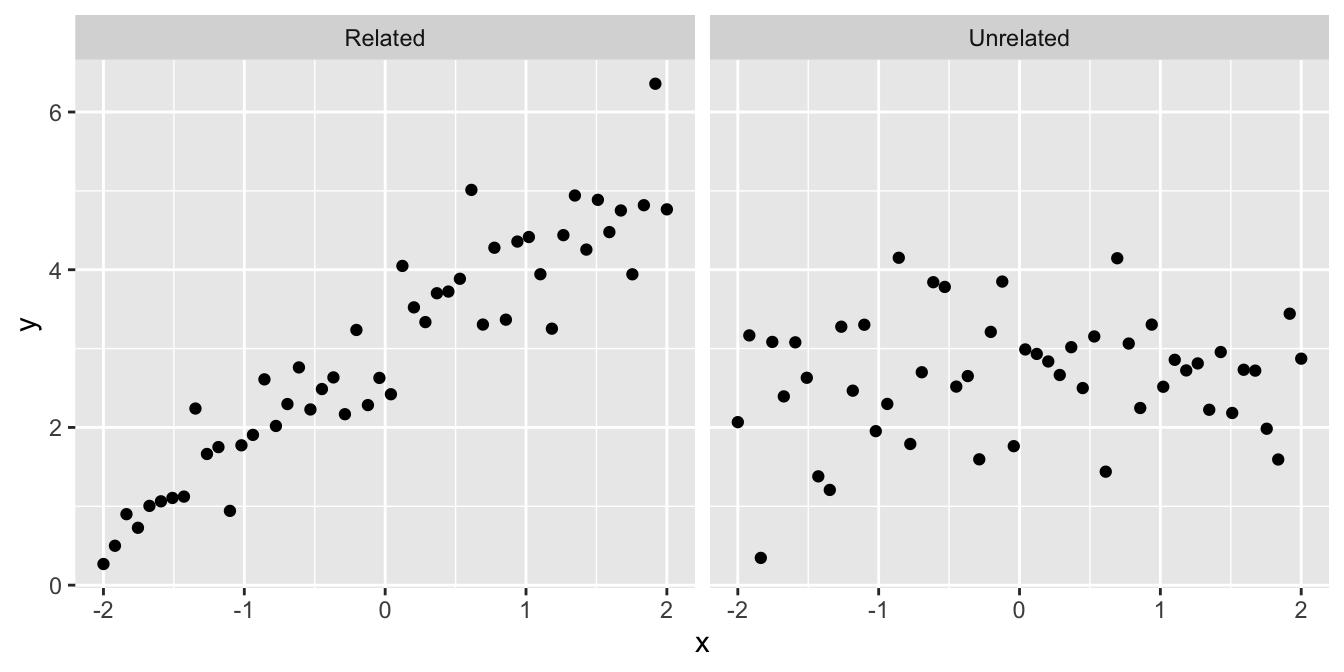
\includegraphics[width=0.6\linewidth]{intro-bio-stats-book_files/figure-latex/reg-eg-related-1} \end{center}

\begin{enumerate}
\def\labelenumi{\arabic{enumi}.}
\setcounter{enumi}{1}
\tightlist
\item
  Is the relationship positive or negative? Sometimes we can answer a scientific question just by knowing the direction of a relationship:
\end{enumerate}

\begin{center}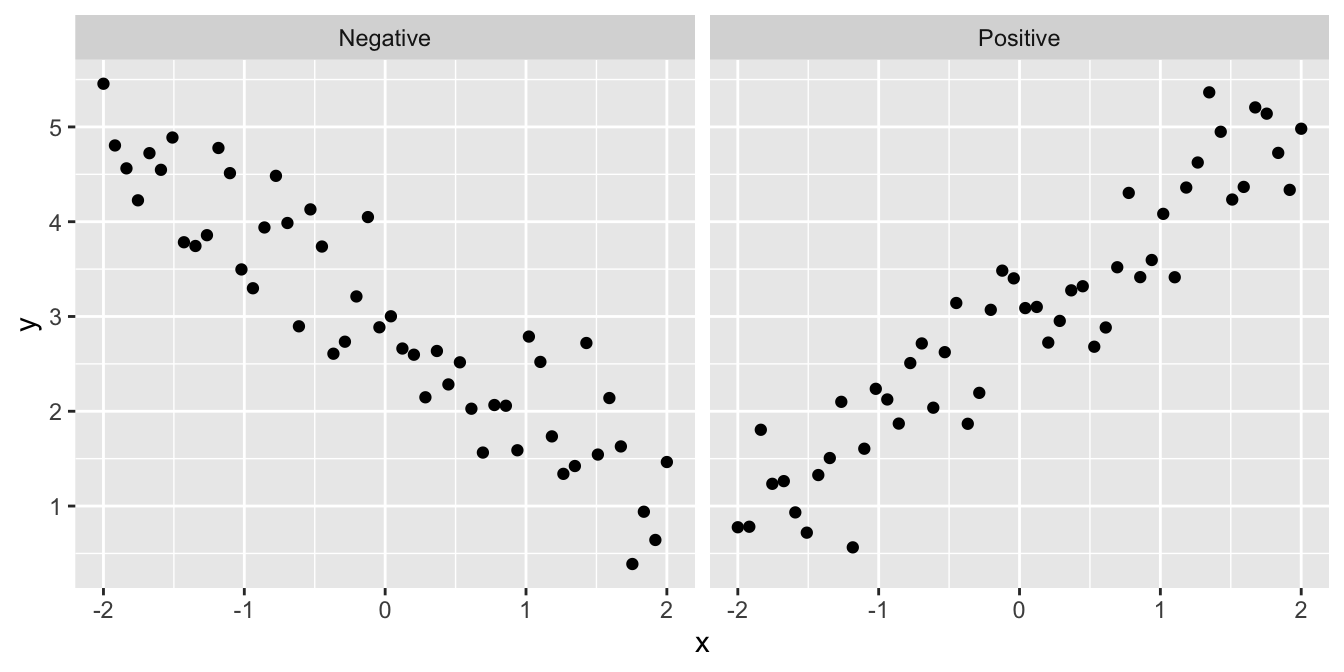
\includegraphics[width=0.6\linewidth]{intro-bio-stats-book_files/figure-latex/reg-eg-posneg-1} \end{center}

\begin{enumerate}
\def\labelenumi{\arabic{enumi}.}
\setcounter{enumi}{2}
\tightlist
\item
  Is the relationship a straight line or a curve? It is important to know the form of a relationship if we want to make predictions:
\end{enumerate}

\begin{center}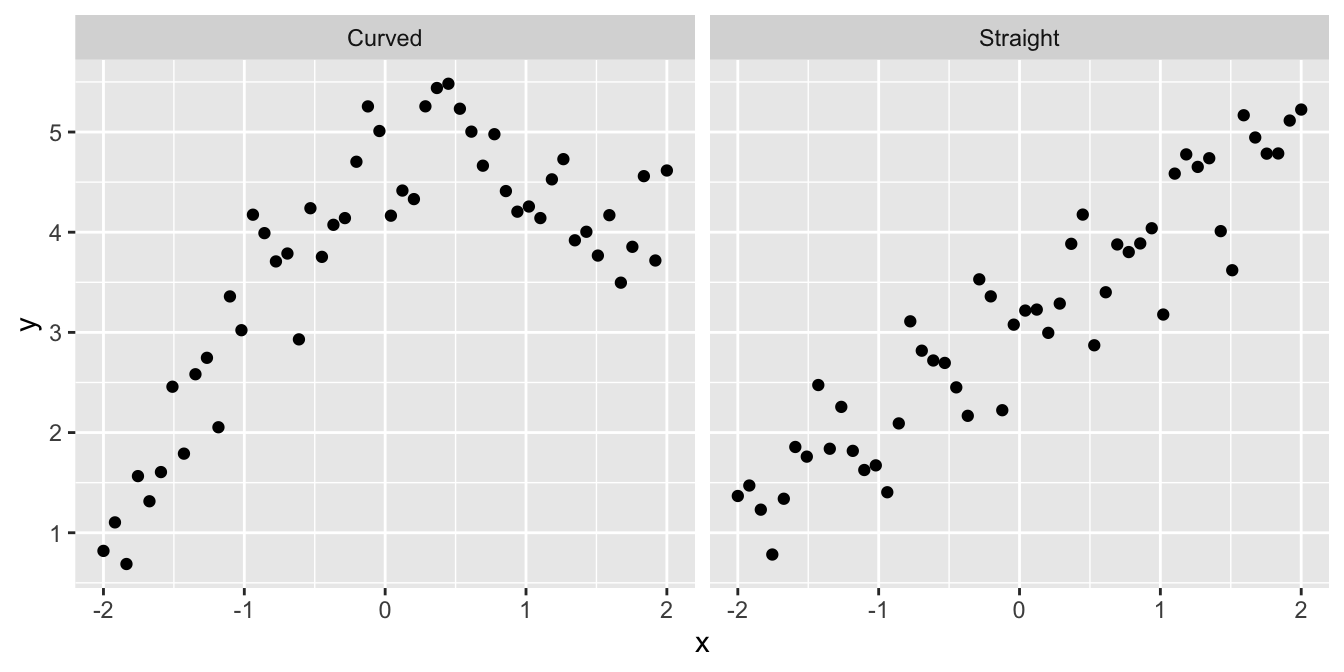
\includegraphics[width=0.6\linewidth]{intro-bio-stats-book_files/figure-latex/reg-eg-linornot-1} \end{center}

Although sometimes it may be obvious that there is a relationship between two variables from a plot of one against the other, at other times it may not. Take a look at the following:

\begin{center}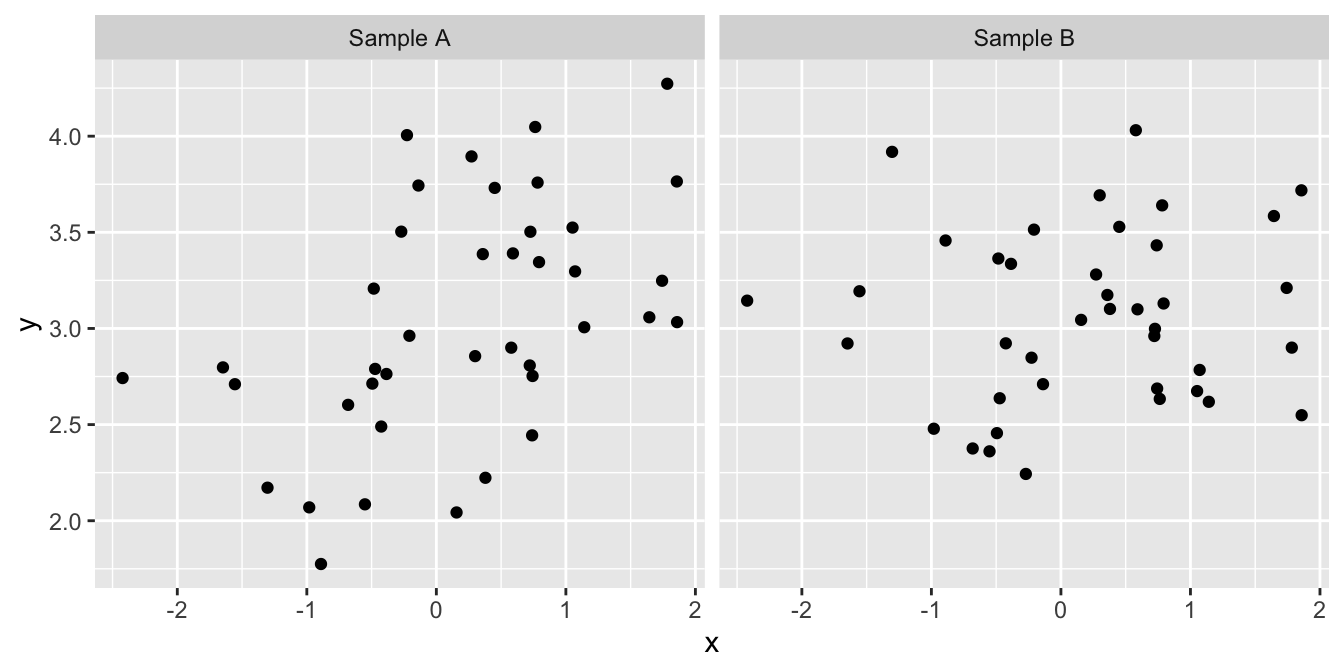
\includegraphics[width=0.7\linewidth]{intro-bio-stats-book_files/figure-latex/reg-eg-confidence-1} \end{center}

We might not be very confident in judging which, if either, of these plots provides evidence of a positive relationship between the two variables. Maybe the pattern we perceive can just be explained by sampling variation, or perhaps it can't. We need a procedure---a statistical test---to evaluate how likely the relationship could have arisen as a result of sampling variation. In addition to judging the statistical significance of a relationship, we may also be interested in describing the relationship mathematically -- i.e.~finding the equation of the best fitting line through the data.

A linear regression analysis allows us to do all this.

\hypertarget{what-does-linear-regression-do}{%
\section{What does linear regression do?}\label{what-does-linear-regression-do}}

\textbf{Simple linear regression} allows us to \emph{predict} how one variable (the \textbf{response variable}) \emph{responds} or \emph{depends} on to another (the \textbf{predictor variable}), assuming a straight-line relationship.

\begin{itemize}
\item
  What does the word `simple' mean here? Simple linear regression is a regression model which only accounts for one predictor variable. If more than one predictor variable is considered, the correct term to describe the resulting model is `multiple regression'. Multiple regression is a very useful tool, but we're only going to study simple regression in this book.
\item
  What does the word `linear' mean here? In statistics, the word linear is used in two slightly different but closely related ways. When discussing simple linear regression, the term linear is often understood to mean that the relationship follows a straight line. That's all. The more technical definition concerns the relationship between the parameters of a statistical model. We don't need to worry about that one here.
\end{itemize}

Writing `simple linear regression' all the time becomes tedious, so we'll often write `linear regression' or `regression'. Just keep in mind that we're always referring to simple linear regression in this book. These regression models account for a straight-line relationship between two numeric variables, i.e.~they describe how the response variable changes in response to the values of the predictor variable. It is conventional to label the response variable as `\(y\)' and the predictor variable as `\(x\)'. When we present such data graphically, the response variable always goes on the \(y\)-axis and the predictor variable on the \(x\)-axis. Try not to forget this convention!

\begin{infobox}{information}

\hypertarget{response-predictor-or-dependent-independent}{%
\subsubsection*{`response / predictor' or `dependent / independent'?}\label{response-predictor-or-dependent-independent}}
\addcontentsline{toc}{subsubsection}{`response / predictor' or `dependent / independent'?}

Another way to describe linear regression is that it finds the straight-line relationship which best describes the dependence of one variable (the \textbf{dependent variable}) on the other (the \textbf{independent variable}). The dependent vs.~independent and response vs.~predictor conventions for variables in a regression are equivalent. They only differ in the words they use to describe the variables involved.

To avoid confusion, we will stick with response / predictor naming convention in this course.

\end{infobox}

How do we decide how to select which is to be used as the response variable and which as the predictor variable? The decision is straightforward in an experimental setting: the manipulated variable is the predictor variable, and the measured outcome is the response variable. Consider the thermal tolerance example from earlier. The temperature was manipulated in that experiment, so it must be designated the predictor variable. Moreover, \emph{a priori} (before conducting the experiment), we can reasonably suppose that temperature changes may cause changes in enzyme activity, but the reverse seems pretty unlikely.

Things are not so clear cut when working with data from an observational study. Indeed, the `response vs predictor' naming convention can lead to confusion because the term `response variable' tends to make people think in terms of causal relationships, i.e.~that variation in the the predictor somehow \emph{causes} changes in the response variable. Sometimes that is true, such as in the experimental setting described above. However, deciding to call one variable a response and the other a predictor should not be taken to automatically imply a casual relationship between them.

Finally, it matters which way round we designate the response and predictor variable in a regression analysis. Suppose we have two variables A and B. In that case, the relationship we find from a regression will not be the same for A against B as for B against A. Choosing which variable to designate as the response boils down to working out which of the variables needs to be explained (response) in terms of the other (predictor).

\hypertarget{how-does-simple-linear-regression-work}{%
\section{How does simple linear regression work?}\label{how-does-simple-linear-regression-work}}

\hypertarget{finding-the-best-fit-line}{%
\subsection{Finding the best fit line}\label{finding-the-best-fit-line}}

If we draw a straight line through a set of points on a graph then, unless they form a perfect straight line, some points will lie close to the line and others further away. The vertical distances between the line and each point (i.e.~measured parallel to the \(y\)-axis) have a special name. They are called the \emph{residuals}. Here's a visual example:

\begin{figure}

{\centering 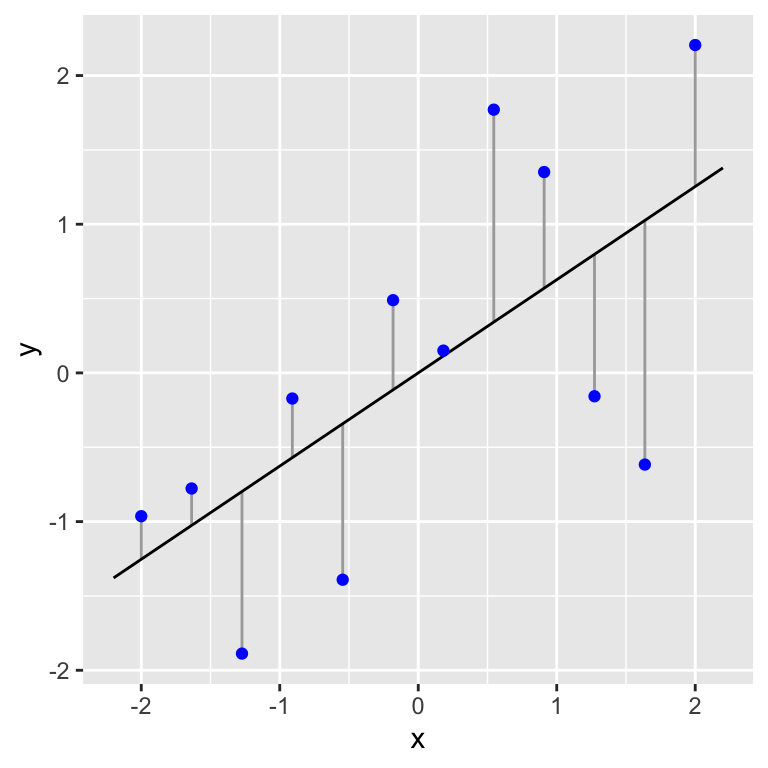
\includegraphics{intro-bio-stats-book_files/figure-latex/reg-eg-with-resids1-1} 

}

\caption{Example of data (blue points) used in a simple regression. A fitted line and the associated residuals (vertical lines) are also shown}\label{fig:reg-eg-with-resids1}
\end{figure}

In this plot the blue points are the data and the vertical lines represent the residuals. The residuals represent the `left over' variation after the line has been fitted through the data. They indicate how well the line fits the data. If all the points lay close to the line, the variability of the residuals would be low relative to the overall variation in the response variable, \(y\). When the observations are more scattered around the line, the variability of the residuals would be large relative to the variation in the response variable, \(y\).

Regression works by finding the line which minimises the size of the residuals in some sense. We'll explain exactly how in a moment. The following illustration indicates the principle of this process:

\begin{center}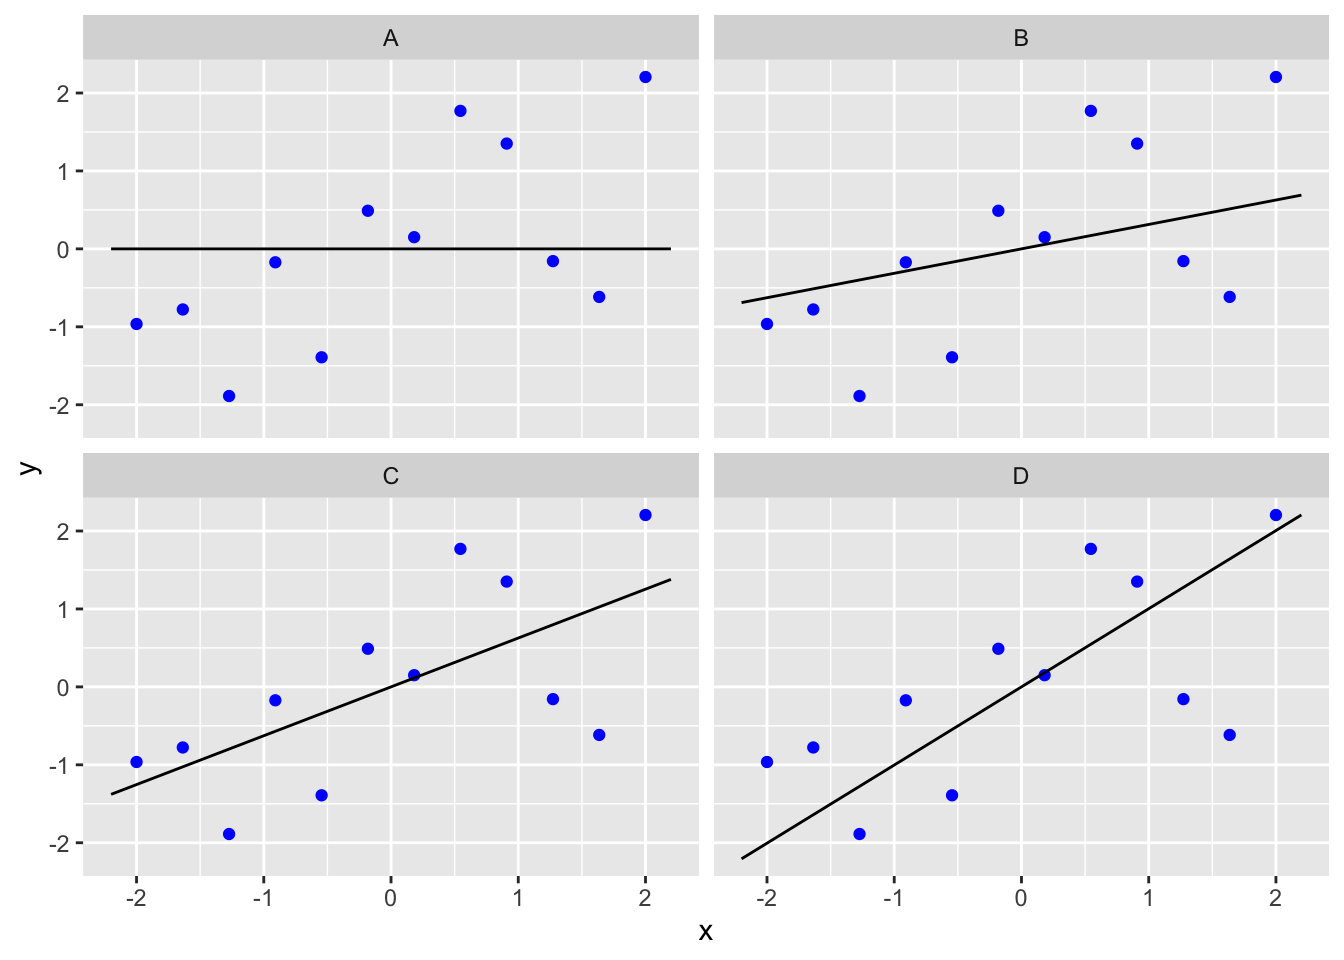
\includegraphics[width=0.7\linewidth]{intro-bio-stats-book_files/figure-latex/reg-eg-four-plots1-1} \end{center}

The data are identical in all four graphs, but in the top left-hand graph a horizontal line (i.e.~no effect of \(x\) on \(y\)) has been fitted, while on the remaining three graphs sloping lines of different magnitude have been fitted.

\begin{infobox}{action}

\hypertarget{which-line-is-best}{%
\subsubsection*{Which line is best?}\label{which-line-is-best}}
\addcontentsline{toc}{subsubsection}{Which line is best?}

One of the four lines is the `line of best' fit from a regression analysis. Spend a few moments looking at the four figures. Which line seems to fit the data best? Why do you think this line is `best'?

\end{infobox}

Let's visualise the data, the candidate lines and the residuals:

\begin{center}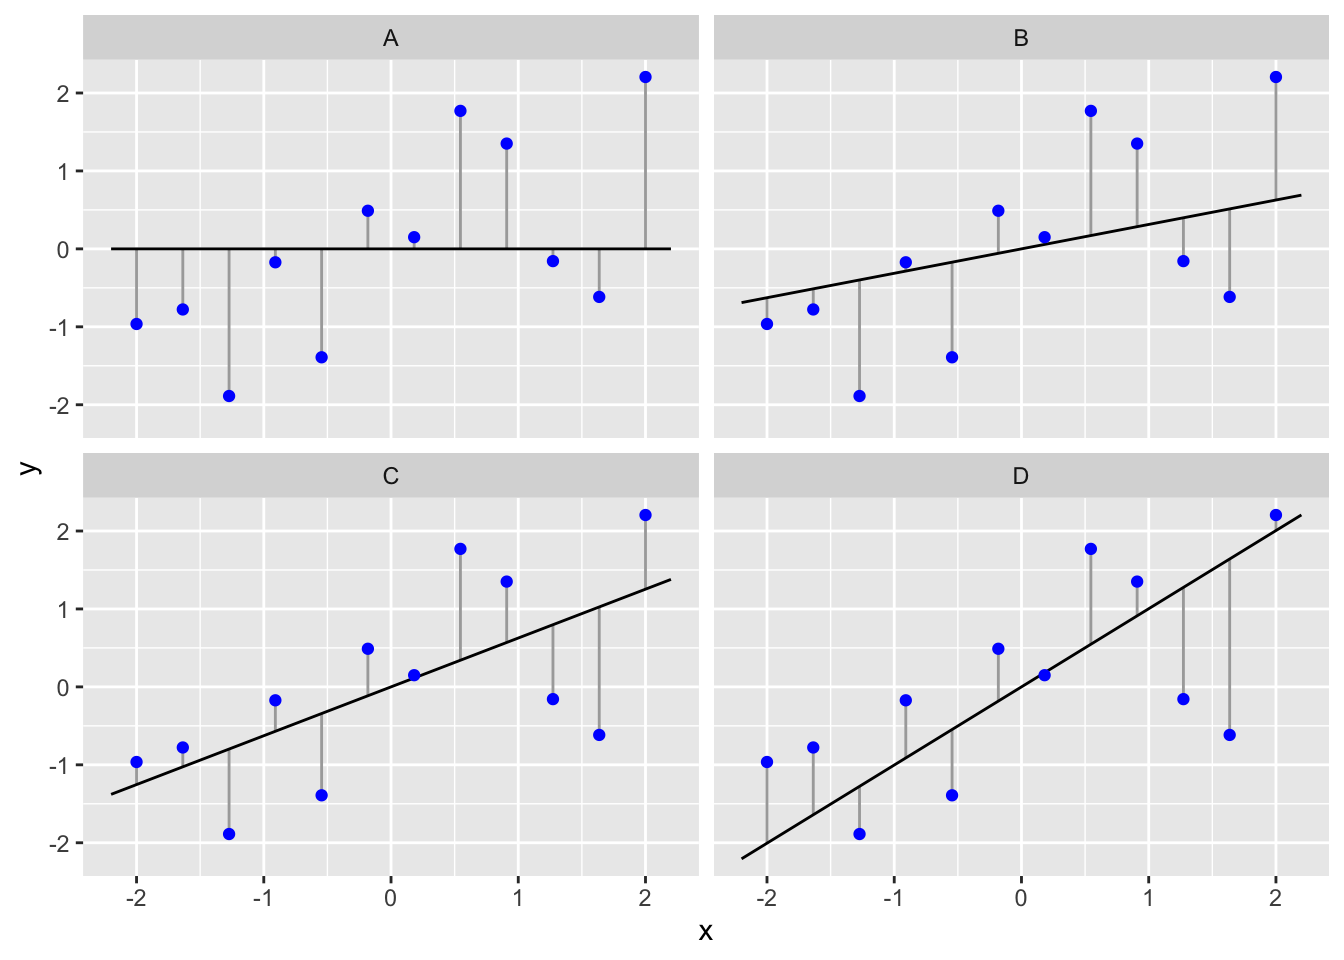
\includegraphics[width=0.7\linewidth]{intro-bio-stats-book_files/figure-latex/reg-eg-four-plots2-1} \end{center}

We said that regression works by finding the intercept and slope that minimises the vertical distances between the line and each observation in some way\footnote{Notice that it is the vertical distance that matters, not the perpendicular distance from the line.}. In fact, it minimises something called the `sum of squares' of these distances: we calculate a sum of squares for a particular set of observations and a fitted line by squaring the residual distances and adding all of these up. This quantity is called the \textbf{residual sum of squares}. The line with the \emph{lowest} residual sum of squares is the best line because it `explains' the most variation in the response variable.

You should be able to see that, for the horizontal line (`A'), the residual sum of squares is larger than any of the other three plots with the sloping lines. This suggests that the sloping lines fit the data better. Which one is best among the three we've plotted? To get at this, we need to calculate the residual sum of squares for each line:

\begin{verbatim}
##   Line    Residual Sum of Squares
## 1    A                   17.55067
## 2    B                   11.97966
## 3    C                   10.12265
## 4    D                   12.79674
\end{verbatim}

So it looks like the line in panel C is the best fitting line among the candidates. In fact, it is the best fit line among all possible candidates. Did you manage to guess this by looking at the lines and the raw data? If not, think about why you got the answer wrong. Did you consider the vertical distances or the perpendicular distances?

\begin{infobox}{warning}

\hypertarget{know-your-residuals}{%
\subsubsection*{Know your residuals}\label{know-your-residuals}}
\addcontentsline{toc}{subsubsection}{Know your residuals}

It is important to understand what a residual represents. Why? Because they pop up all the time when working with statistical models (not only regression, in fact). It is hard to understand what R is telling you about a model without knowing about these residual things.

\end{infobox}

\hypertarget{what-do-you-get-out-of-a-regression}{%
\section{What do you get out of a regression?}\label{what-do-you-get-out-of-a-regression}}

A regression analysis involves two activities:

\begin{itemize}
\item
  \textbf{Interpretation.} When we `fit' a regression model to data we estimate the coefficients of a best-fit straight line through the data. This is the equation that best describes how the \(y\) (response) variable \emph{responds to} the \(x\) (predictor) variable. To put it in slightly more technical terms, it describes the \(y\) variable as a function of the \(x\) variable. This model may be used to understand how the variables are related or make predictions.
\item
  \textbf{Inference.} It is not enough to just estimate the regression equation. Before we can use it, we need to determine whether there is a statistically significant relationship between the \(x\) and \(y\) variables. That is, the analysis will tell us whether an apparent association is likely to be real or just a chance outcome resulting from sampling variation.
\end{itemize}

\hypertarget{interpreting-a-regression}{%
\subsection{Interpreting a regression}\label{interpreting-a-regression}}

What is the form of the relationship? The equation for a straight-line relationship is \(y = a + b \times x\), where

\begin{itemize}
\item
  \(y\) is the response variable,
\item
  \(x\) is the predictor variable,
\item
  \(a\) is the intercept (i.e.~where the line crosses the \(y\) axis), and
\item
  \(b\) is the slope of the line.
\end{itemize}

The \(a\) and the \(b\) are referred to as the \emph{coefficients} (or \emph{parameters}) of the line. The slope of the line is often the coefficient we care about most. It tells us the amount by which \(y\) changes for a change of one unit in \(x\). If the value of \(b\) is positive (i.e.~a plus sign in the above equation) this means the line slopes upwards to the right. A negative slope (\(y = a - bx\)) means the line slopes downwards to the right. The diagram below shows the derivation of an equation for a straight line.

\begin{center}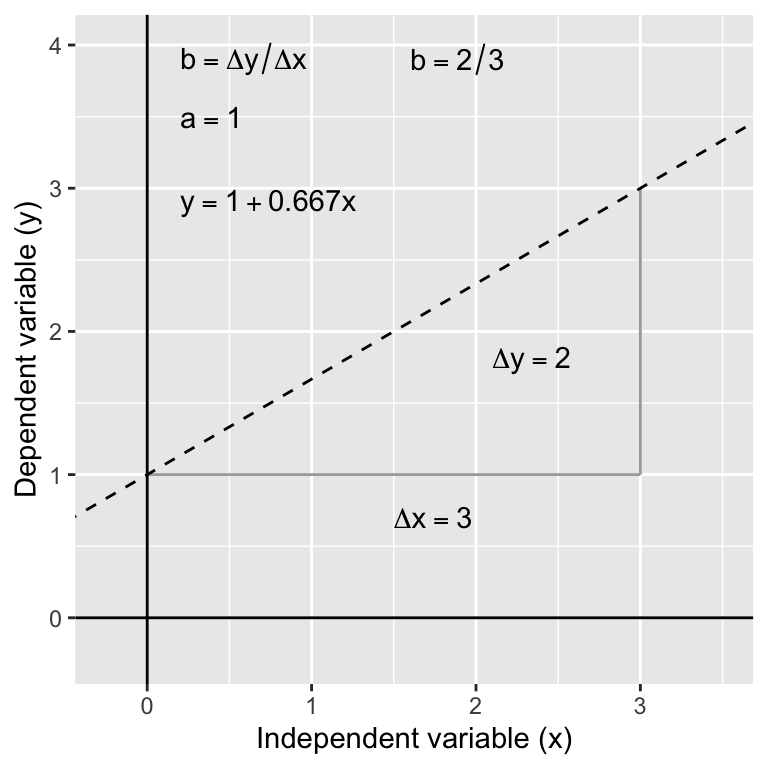
\includegraphics{intro-bio-stats-book_files/figure-latex/reg-line-explain-1} \end{center}

Having the equation for a relationship allows us to predict the value of the \(y\) variable for any value of \(x\). For example, in the thermal tolerance example, we want an equation that will allow us to work out how fitness changes with temperature. Such predictions can be made by hand (see below) or using R (details later).

In the above diagram, the regression equation is: \(y = 1 + 0.66 x\). So to find the value of \(y\) at \(x = 2\) we use: \(y = 1 + (0.667 \times 2) = 2.32\). Obviously, by finding \(y\) values for 2 (or preferably 3) different \(x\) values from the equation, the actual line can easily be plotted on a graph manually if required---plot the values and join the dots! It's much easier to use R to do this kind of thing though.

\begin{infobox}{information}

\hypertarget{regression-involves-a-statistical-model}{%
\subsubsection*{Regression involves a statistical model}\label{regression-involves-a-statistical-model}}
\addcontentsline{toc}{subsubsection}{Regression involves a statistical model}

A simple linear regression is underpinned by a statistical model. If you skim back through the \protect\hyperlink{parametric-statistics}{parametric statistics} chapter, you will see that the equation \(y = a + b \times x\) represents the `systematic component' of the regression model. This bit describes the component of variation in \(y\) that is explained by the model for the dependence of \(y\) on \(x\). The residuals correspond to the `random component' of the model. These represent the component of variation in the \(y\) variable that our regression model fails to describe.

\end{infobox}

\hypertarget{evaluating-hypotheses-inference}{%
\subsection{Evaluating hypotheses (`inference')}\label{evaluating-hypotheses-inference}}

More than one kind of significance test can be carried out with a simple linear regression. We're going to focus on the most common test: an \emph{F} test of whether the slope coefficient is significantly different from 0. This addresses the important question, ``Is there a relationship?''

How do we do this? We play exactly the same kind of gambit we used to develop the earlier significance tests:

\begin{enumerate}
\def\labelenumi{\arabic{enumi}.}
\item
  We start with a null hypothesis of `no effect'. This corresponds to the hypothesis that the slope of the regression is zero.
\item
  We then work out what the distribution of some kind of test statistic should look like under the null hypothesis. The test statistic in this case is called the \emph{F}-ratio.
\item
  We then calculate a \emph{p}-value by asking how likely it is that we would see the observed test statistic, or a more extreme value, if the null hypothesis were really true.
\end{enumerate}

It's not so critical that someone understands the mechanics of an \emph{F}-test to use it. However, knowing a bit about where is comes from does help to demystify the output produced by R. To that end, let's step through the calculations involved in the \emph{F} test using the example data shown in the above four-panel plot.

\hypertarget{total-variation}{%
\subsubsection*{Total variation}\label{total-variation}}
\addcontentsline{toc}{subsubsection}{Total variation}

We first need to calculate something called the \textbf{total sum of squares}. The figure below shows the raw data (blue points) and the grand mean (i.e.~the sample mean).

\begin{center}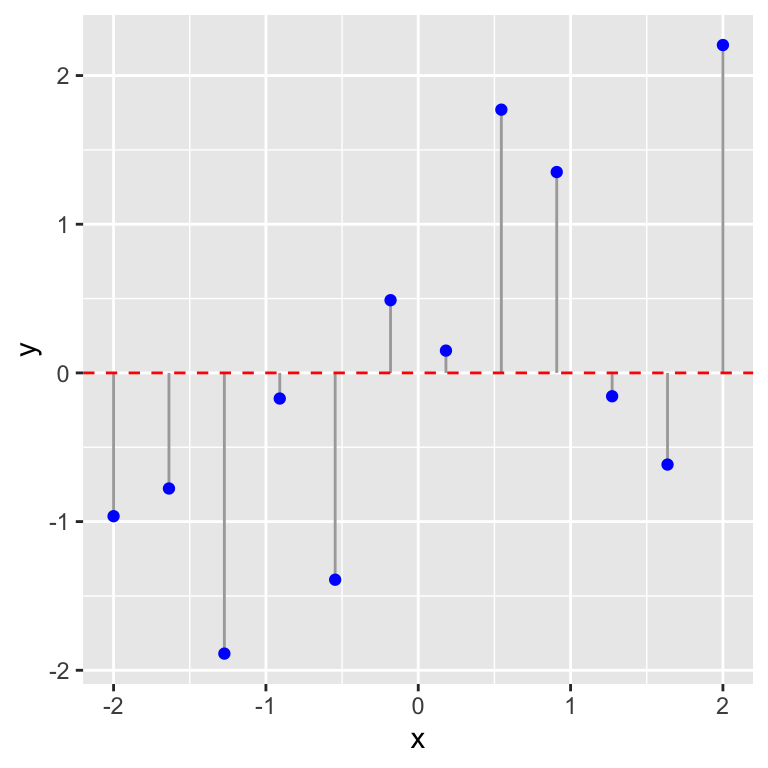
\includegraphics{intro-bio-stats-book_files/figure-latex/reg-eg-total-1} \end{center}

The vertical lines show the distance between each observation and the grand mean. These vertical lines are just the residuals from a model where the slope of the line is set to zero. What we need to do is quantify the variability of these residuals. We can't just add them up, because by definition, they have to sum to zero, i.e.~they are calculated relative to the grand mean.

Instead, we calculate the total sum of squares by taking each residual in turn, squaring it, and then adding up all the squared values. We call this the total sum of squares because it is a measure of the total variability in the response variable, \(y\). This number is 17.55 for the data in the figure above.

\hypertarget{residual-variation}{%
\subsubsection*{Residual variation}\label{residual-variation}}
\addcontentsline{toc}{subsubsection}{Residual variation}

Next we need to calculate the \textbf{residual sum of squares}. We have already seen how this calculation works because it is used in the calculation of the best fit line---the best fit line is the one that minimises the residual sum of squares. Let's plot this line along with the associated residuals of this line again:

\begin{center}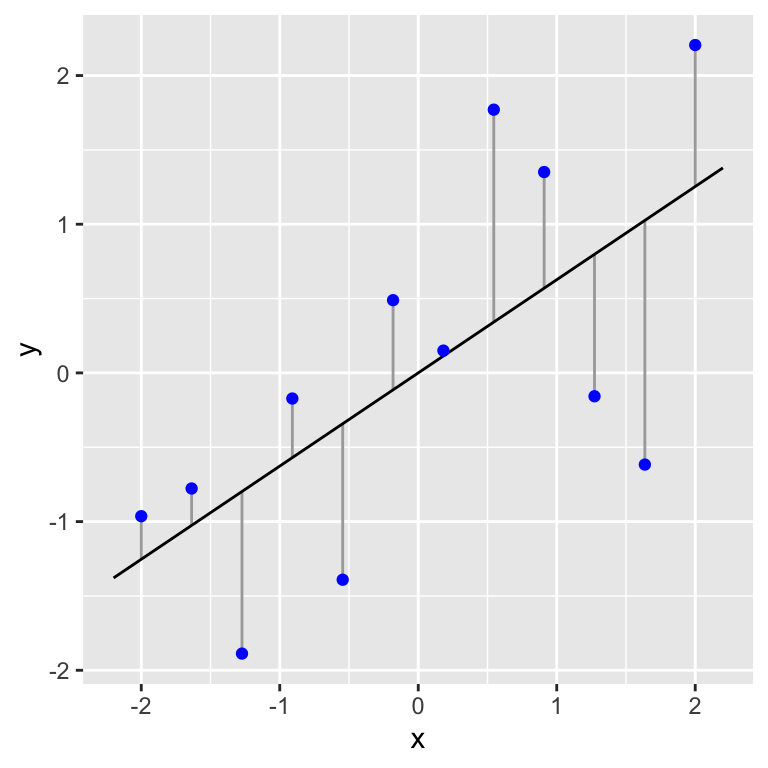
\includegraphics{intro-bio-stats-book_files/figure-latex/reg-eg-with-resids2-1} \end{center}

The vertical lines show the distance between each observation and the best fit line. We need to quantify the variability of these residuals. Again, we can't just add up the deviations because they have to sum to zero as a result of how the best fit line is found. Instead we calculate the residual sum of squares by taking each residual in turn, squaring it, and then adding up all the squared values. This number is 10.12 for the figure above. We call this the residual, or error, sum of squares because it is a measure of the variation in \(y\) that is `left over' after accounting for the influence of the predictor variable \(x\).

\hypertarget{explained-variation}{%
\subsubsection*{Explained variation}\label{explained-variation}}
\addcontentsline{toc}{subsubsection}{Explained variation}

Once the total sum of squares and the residual sum of squares are known, we can calculate the quantity we really want: the \textbf{explained sum of squares}. This is a measure of the variation in \(y\) that is explained by the influence of the predictor variable \(x\). We calculate this by subtracting the residual sum of squares from the total sum of squares. This makes intuitive sense: if we subtract the variation in \(y\) we can't explain (residual) from all the variation in \(y\) (total), we end up with the amount `explained' by the regression. This number is 7.43 for the example.

\hypertarget{degrees-of-freedom-mean-squares-and-f-tests}{%
\subsubsection*{\texorpdfstring{Degrees of freedom, mean squares and \emph{F} tests}{Degrees of freedom, mean squares and F tests}}\label{degrees-of-freedom-mean-squares-and-f-tests}}
\addcontentsline{toc}{subsubsection}{Degrees of freedom, mean squares and \emph{F} tests}

The problem with sums of squares is that they are a function of sample size. The more data we have, the larger our sum of squares will get. The solution to this problem is to convert them into a measure of variability that doesn't scale with sample size. We need to calculate \textbf{degrees of freedom} (written as df, or d.f.) to do this. We came across the concept of degrees of freedom when we studied the \emph{t}-test. The idea is closely related to sample size. It is difficult to give a precise definition, but roughly speaking, the degrees of freedom of a statistic is a measures of how much information it is based on (bigger is better).

Each of the measures of variability we just calculated for the simple linear regression has a degrees of freedom associated with it. We need the explained and error degrees of freedom:

\begin{itemize}
\item
  Explained d.f. = 1
\item
  Error d.f. = (Number of observations - 2)
\end{itemize}

Don't worry if those seem a little cryptic. We don't need to carry out degrees of freedom calculations by hand because R will do them for us. We'll think about degrees of freedom a bit more when we start to learn about ANOVA models.

The reason degrees of freedom matter is because we can use them to standardise the sum of squares to account for sample size. The calculations are very simple. We take each sum of squares and divide it by its associated degrees of freedom. The resulting quantity is called a \textbf{mean square} (it's the mean of squared deviations): \[
\text{Mean Square} = \frac{\text{Sum of Squares}}{\text{Degrees of Freedom}}
\] A mean square is actually an estimate of variance. Remember the variance? It is one of the standard measures of a distribution's dispersion, or spread.

Now for the important bit. The two mean squares can be compared by calculating the ratio between them, which is designated by the letter \emph{F}:

\[F = \mbox{Variance Ratio} = \frac{\mbox{Explained Mean Square}}{\mbox{Residual Mean Square}}\]

This is called the \emph{F} ratio, or sometimes, the variance ratio. If the explained variation is large compared to the residual variation, then the \emph{F} ratio will be large. Conversely, if the explained variation is relatively small the \emph{F} ratio will be small. We can see where this is heading\ldots{}

The \emph{F} ratio is a type of test statistic---if the value of \emph{F} is sufficiently large, we judge it to be statistically significant. For this judgement to be valid, we have to make one key assumption about the population from which the data has been sampled: we assume the residuals are drawn from a normal distribution. If this assumption is correct, it can be shown that the distribution of the \emph{F} ratio under the null hypothesis (the `null distribution') has a particular form: it follows a theoretical distribution called an \emph{F}-distribution. And yes, that's why the variance ratio is called `\emph{F}'.

All this means we can assess statistical significance of the slope coefficient by comparing the \emph{F} ratio calculated from a sample to this theoretical distribution. This procedure is called an \emph{F} test. The \emph{F} ratio is 7.34 in our example. This is quite high, which indicates that the slope is likely to be significantly different from 0.

We need more than an \emph{F} ratio to calculate a \emph{p}-value. We also need to consider the degrees of freedom of the test. Furthermore, because this test involves an \emph{F} ratio, \textbf{there are two different degrees of freedom to consider}: the explained and residual df's. Try to remember that fact---\emph{F} ratio tests involve a pair of degrees of freedom.

We could calculate a \emph{p}-value now by messing around with tables of \emph{F} ratios and degrees of freedom. However, it is much easier to let R do this for us when working with a regression model. That's what we're going to do in the next chapter, so for now, we'll leave significance tests alone.

\hypertarget{correlation-or-regression}{%
\section{Correlation or regression?}\label{correlation-or-regression}}

Before we finish up, it is worth pausing to review the difference between regression and correlation analyses. Whilst regression and correlation are both concerned with associations between numeric variables, they are different techniques and each is appropriate under distinct circumstances. This is a frequent source of confusion. Which technique is required for a particular analysis depends on

\begin{itemize}
\tightlist
\item
  the way the data were collected and
\item
  the goal of the analysis.
\end{itemize}

There are two broad questions to consider---

\hypertarget{where-do-the-data-come-from}{%
\subsubsection*{Where do the data come from?}\label{where-do-the-data-come-from}}
\addcontentsline{toc}{subsubsection}{Where do the data come from?}

Think about how the data have been collected. If they are from a study where one of the variables has been experimentally manipulated, then choosing the best analysis is easy. We should use a regression analysis, in which the predictor variable is the experimentally manipulated variable and the response variable is the measured outcome. The fitted line from a regression analysis describes how the outcome variable \emph{depends on} the manipulated variable---it describes the causal relationship between them.

It is generally inappropriate to use correlation to analyse data from an experimental setting. A correlation analysis examines association but does not imply the dependence of one variable on another. Since there is no distinction of response or predictor variables, it doesn't matter which way round we do a correlation. In fact, the phrase `which way round' doesn't even make sense in the context of a correlation.

If the data are from a so-called `observational study' where someone took measurements, but nothing was actually manipulated experimentally, then either method may be appropriate.

\hypertarget{what-is-the-goal-of-the-analysis}{%
\subsubsection*{What is the goal of the analysis?}\label{what-is-the-goal-of-the-analysis}}
\addcontentsline{toc}{subsubsection}{What is the goal of the analysis?}

Think about what question is being asked. A correlation coefficient only quantifies the strength and direction of an association between variables---it tells us nothing about the form of a relationship. Nor does it allow us to make predictions about the value of one variable from the values of a second. A regression does allow this because it involves fitting a line through the data---i.e.~regression involves \textbf{a model} for the relationship.

This means that if the goal is to understand the form of a relationship between two variables, or to use a fitted model to make predictions, we have to use regression. If we just want to know whether two variables are associated or not, the direction of the association, and whether the association is strong or weak, then a correlation analysis is sufficient. It is better to use a correlation analysis when the extra information produced by a regression is not needed, because the former will be simpler and potentially more robust.

\hypertarget{regression-in-R}{%
\chapter{Simple regression in R}\label{regression-in-R}}

Our goal in this chapter is to learn how to work with regression models in R. We'll start with the example problem and the data, and then work through model fitting, significance testing, and finally, presenting the results.

\hypertarget{introduction-2}{%
\section{Introduction}\label{introduction-2}}

A plant physiologist studying the process of germination in the broad bean (\emph{Vicia faba}) is interested in the relationship between the activity of the enzyme amylase and the temperature at which the germinating beans are kept. As part of this work, she carries out an experiment to find the relationship between glucose release (from the breakdown of starch by amylase) and temperature (over the range 2 - 20C). The data obtained from such an experiment are given below.

\begin{longtable}[]{@{}lllllllllll@{}}
\toprule
& & & & & & & & & & \\
\midrule
\endhead
Temperature (\(C\)) & 2 & 4 & 6 & 8 & 10 & 12 & 14 & 16 & 18 & 20 \\
Glucose (\(\mu g\) \(mg^{-1}\) dry weight) & 1.0 & 0.5 & 2.5 & 1.5 & 3.2 & 4.3 & 2.5 & 3.5 & 2.8 & 5.6 \\
\bottomrule
\end{longtable}

We want to work out whether there a statistically significant relationship between temperature and glucose release (and hence, presumably, amylase activity). That's a job for linear regression.

\begin{infobox}{action}

\hypertarget{section-6}{%
\subsubsection*{}\label{section-6}}
\addcontentsline{toc}{subsubsection}{}

We will be using this new data set to demonstrate how to conduct simple regression in R. The data live in the `GLUCOSE.CSV' file. The code below assumes those data have been read into a tibble called \texttt{vicia\_germ}. Set that up if you plan to work along.

\end{infobox}

\hypertarget{first-steps}{%
\subsection{First steps}\label{first-steps}}

We start by using \texttt{glimpse} to see what resides within \texttt{vicia\_germ}:

\begin{Shaded}
\begin{Highlighting}[]
\FunctionTok{glimpse}\NormalTok{(vicia\_germ)}
\end{Highlighting}
\end{Shaded}

\begin{verbatim}
## Rows: 10
## Columns: 2
## $ Temperature <dbl> 2, 4, 6, 8, 10, 12, 14, 16, 18, 20
## $ Glucose     <dbl> 1.0, 0.5, 2.5, 1.5, 3.2, 4.3, 2.5, 3.5, 2.8, 5.6
\end{verbatim}

There are just two numeric variables. The first column (\texttt{Temperature}) contains the information about the experimental temperature treatments, and the second column (\texttt{Glucose}) contain the glucose measurements.

Notice that we refer to the different temperatures as `experimental treatments'. This is because these data are from an experiment where temperature was controlled by the investigator. We'll discuss this terminology in more detail in the \protect\hyperlink{principles-experimental-design}{Principles of Experimental Design} chapter.

\hypertarget{visualising-the-data}{%
\subsection{Visualising the data}\label{visualising-the-data}}

We should visualise the data next so that we understand it more. A simple scatter plot will do:

\begin{Shaded}
\begin{Highlighting}[]
\FunctionTok{ggplot}\NormalTok{(vicia\_germ, }\FunctionTok{aes}\NormalTok{(}\AttributeTok{x =}\NormalTok{ Temperature, }\AttributeTok{y =}\NormalTok{ Glucose)) }\SpecialCharTok{+} 
  \FunctionTok{geom\_point}\NormalTok{()}
\end{Highlighting}
\end{Shaded}

\begin{center}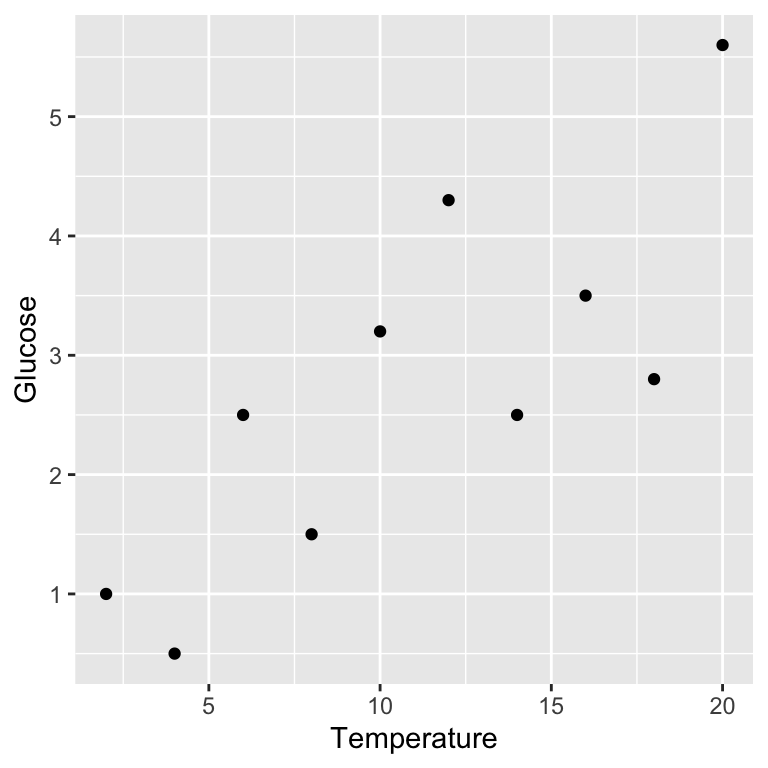
\includegraphics[width=0.5\linewidth]{intro-bio-stats-book_files/figure-latex/reg-worked-scatterplot-1} \end{center}

Remember, \texttt{Glucose} is the response variable and \texttt{Temperature} is the predictor variable, so they belong on the \(y\) and \(x\) axes, respectively.

\begin{infobox}{warning}

\hypertarget{variables-and-axes}{%
\subsubsection*{Variables and axes}\label{variables-and-axes}}
\addcontentsline{toc}{subsubsection}{Variables and axes}

Be careful when you produce a scatter plot to summarise data in a regression analysis. You need to make sure the two variables are plotted the right way around with respect to the \(x\) and \(y\) axes: place the response variable on the \(y\) axis and the predictor on the \(x\) axis. Nothing says, ``I don't know what I'm doing,'' quite like mixing up the axes.

\end{infobox}

Because linear regression involves fitting a straight line through our data, it only makes sense to fit this model if the relationship between the two variables is linear. Plotting our data lets us see whether or not there appears to be a linear relationship. The scatter plot we produced above suggests that, in this case, the relationship between \(x\) and \(y\) is linear.

\begin{infobox}{warning}

\hypertarget{assumptions}{%
\subsubsection*{Assumptions}\label{assumptions}}
\addcontentsline{toc}{subsubsection}{Assumptions}

A linear relationship between the predictor and response variables is not the only assumption that we have to make when we fit a linear regression. We'll come back to the other assumptions and how to check whether they have been met in the \protect\hyperlink{assumptions-diagnostics}{Assumptions} and \protect\hyperlink{regression-diagnostics}{Diagnostics} chapters, respectively. For now you should just be aware that there are assumptions that you should check when working with your own data.

\end{infobox}

\hypertarget{model-fitting-and-significance-tests}{%
\section{Model fitting and significance tests}\label{model-fitting-and-significance-tests}}

Carrying out a regression analysis in R is a two step process.

The first step involves a process known as \emph{fitting the model} (or just \emph{model fitting}). In effect, this is the step where R calculates the best fit line, along with a large amount of additional information needed to generate the results in step two. We call this step model fitting because, well, we end up fitting the straight line model to the data.

How do we fit a linear regression model in R? We will do it using the \texttt{lm} function. The letters `lm' in this function name stand for `linear model'. We won't say much more at this point other than point out that a linear regression is a particular case of a general linear model. R doesn't have a special regression function.

Here is how we fit a linear regression in R using the enzyme data:

\begin{Shaded}
\begin{Highlighting}[]
\NormalTok{vicia\_model }\OtherTok{\textless{}{-}} \FunctionTok{lm}\NormalTok{(Glucose }\SpecialCharTok{\textasciitilde{}}\NormalTok{ Temperature, }\AttributeTok{data =}\NormalTok{ vicia\_germ)}
\end{Highlighting}
\end{Shaded}

This should look quite familiar. We have to assign two arguments:

\begin{enumerate}
\def\labelenumi{\arabic{enumi}.}
\item
  The first argument is a \textbf{formula}. We know this because it includes a `tilde' symbol: \texttt{\textasciitilde{}}. The variable name on the left of the \texttt{\textasciitilde{}} should be the response variable. The variable name on the right should be the predictor variable. These are \texttt{Glucose} and \texttt{Temperature}, respectively. Make sure you get these the right way round when carrying out regression.
\item
  The second argument is the name of the data frame or tibble object that contains the two variables listed in the formula (\texttt{vicia\_germ}).
\end{enumerate}

\begin{infobox}{information}

\hypertarget{how-does-r-knows-we-want-to-carry-out-a-regression}{%
\subsubsection*{How does R knows we want to carry out a regression?}\label{how-does-r-knows-we-want-to-carry-out-a-regression}}
\addcontentsline{toc}{subsubsection}{How does R knows we want to carry out a regression?}

How does R know we want to use regression? After all, we didn't specify this anywhere. The answer is that R looks at what type of variable \texttt{Temperature} is. It is numeric, and so R automatically carries out a regression. If it had been a factor or a character vector (representing a categorical variable), R would have carried out a different kind of analysis, called a one-way Analysis of Variance (ANOVA). Many of the models we examine in this course are very similar and can be fitted using the \texttt{lm} function. The only thing that really distinguishes them is the type of variables that appear to the right of the \texttt{\textasciitilde{}} in a formula: if they are categorical variables, we end up fitting an ANOVA model, while numeric variables lead to a regression.

The key message is that you have to keep a close eye on the type of variables you are modelling to understand what kind of model R will fit.

\end{infobox}

Notice that we did not print the results to the console. Instead, we assigned the result a name (\texttt{vicia\_model}). This now refers to a fitted \textbf{model object}. What happens if we print a regression model object to the console?

\begin{Shaded}
\begin{Highlighting}[]
\FunctionTok{print}\NormalTok{(vicia\_model)}
\end{Highlighting}
\end{Shaded}

\begin{verbatim}
## 
## Call:
## lm(formula = Glucose ~ Temperature, data = vicia_germ)
## 
## Coefficients:
## (Intercept)  Temperature  
##      0.5200       0.2018
\end{verbatim}

This prints a quick summary of the model we fitted and some information about the `coefficients' of the model. The coefficients are the intercept and slope of the fitted line: the intercept is always labelled \texttt{(Intercept)} and the slope is labelled with the name of the predictor variable (\texttt{Temperature} in this case). We'll come back to these coefficients once we have looked at how to compute \emph{p}-values.

The second step of a regression analysis involves using the fitted model to assess statistical significance. We usually want to determine whether the slope is significantly different from zero. That is, we want to know if the relationship between the \(x\) and \(y\) variables is likely to be real or just the result of sampling variation. Carrying out the required \emph{F} test is actually very easy. The test relies on a function called \texttt{anova}. To use this function, all we have to do is pass it one argument---the name of the fitted regression model object:

\begin{Shaded}
\begin{Highlighting}[]
\FunctionTok{anova}\NormalTok{(vicia\_model)}
\end{Highlighting}
\end{Shaded}

\begin{verbatim}
## Analysis of Variance Table
## 
## Response: Glucose
##             Df  Sum Sq Mean Sq F value   Pr(>F)   
## Temperature  1 13.4411 13.4411  14.032 0.005657 **
## Residuals    8  7.6629  0.9579                    
## ---
## Signif. codes:  0 '***' 0.001 '**' 0.01 '*' 0.05 '.' 0.1 ' ' 1
\end{verbatim}

Let's step through the output to see what it means. The first line informs us that we are looking at an Analysis of Variance Table---a set of statistical results derived from a general tool called Analysis of Variance. The second line reminds us what response variable we analysed (\texttt{Glucose}). Those parts are simple to describe at least, though the Analysis of Variance reference may seem a little cryptic. In a nutshell, every time we carry out an \emph{F}-test we are performing some kind of Analysis of Variance because the test boils down to a ratio of two variances.

The important part of the output is the table at the end:

\begin{verbatim}
##             Df  Sum Sq Mean Sq F value   Pr(>F)    
## Temperature  1 13.4411 13.4411  14.032 0.005657 ** 
## Residuals    8  7.6629  0.9579
\end{verbatim}

This summarises the different parts of the \emph{F}-test calculations: \texttt{Df} -- degrees of freedom, \texttt{Sum\ Sq} -- the sum of squares, \texttt{Mean\ Sq} -- the mean square, \texttt{F\ value} -- the \emph{F}-statistic, \texttt{Pr(\textgreater{}F)} -- the p-value. These were touched on in the last chapter.

The \emph{F}-statistic (variance ratio) is the key term. When working with a regression model, this quantifies how much variability in the data is explained when we include the best fit slope term in the model. Larger values indicate a stronger relationship between \(x\) and \(y\). The \emph{p}-value gives the probability that the relationship could have arisen through sampling variation if there were no real association. As always, a \emph{p}-value of less than 0.05 is taken as evidence that the relationship is real, i.e.~the result is statistically significant.

We should also note down the two degrees of freedom given in the table because these will be needed when we report the results.

\hypertarget{extracting-a-little-more-information}{%
\subsection{Extracting a little more information}\label{extracting-a-little-more-information}}

There is a second function, called \texttt{summary}, that can be used to extract a little more information from the fitted regression model:

\begin{Shaded}
\begin{Highlighting}[]
\FunctionTok{summary}\NormalTok{(vicia\_model)}
\end{Highlighting}
\end{Shaded}

\begin{verbatim}
## 
## Call:
## lm(formula = Glucose ~ Temperature, data = vicia_germ)
## 
## Residuals:
##      Min       1Q   Median       3Q      Max 
## -1.35273 -0.77909 -0.08636  0.74227  1.35818 
## 
## Coefficients:
##             Estimate Std. Error t value Pr(>|t|)   
## (Intercept)  0.52000    0.66858   0.778  0.45909   
## Temperature  0.20182    0.05388   3.746  0.00566 **
## ---
## Signif. codes:  0 '***' 0.001 '**' 0.01 '*' 0.05 '.' 0.1 ' ' 1
## 
## Residual standard error: 0.9787 on 8 degrees of freedom
## Multiple R-squared:  0.6369, Adjusted R-squared:  0.5915 
## F-statistic: 14.03 on 1 and 8 DF,  p-value: 0.005657
\end{verbatim}

This is easiest to understand if we step through the constituent parts of the output. The first couple of lines just remind us about the model we fitted

\begin{verbatim}
## Call: 
## lm(formula = Glucose ~ Temperature, data = vicia_germ)
\end{verbatim}

The next couple of lines aren't really all that useful---they summarise some properties of the residuals--so we'll ignore these.

The next few lines comprise a table that summarises some useful information about the coefficients of the model (the intercept and slope):

\begin{verbatim}
## Coefficients: 
##             Estimate Std. Error t value Pr(>|t|)    
## (Intercept)  0.52000    0.66858   0.778  0.45909    
## Temperature  0.20182    0.05388   3.746  0.00566 **
\end{verbatim}

The \texttt{Estimate} column shows us the estimated intercept and slope of the regression. We saw these earlier when we printed the fitted model object to the console.

Staying with this table, the next three columns (\texttt{Std.\ Error}, \texttt{t\ value} and \texttt{Pr(\textgreater{}\textbar{}t\textbar{})}) show us the standard error associated with each coefficient, the corresponding \emph{t}-statistics, and the \emph{p}-values. Remember standard errors? These measure the uncertainty of the sampling distributions associated with various estimates from a sample. We discussed standard errors in the context of sample means. One can calculate a standard error for many different kinds of quantities, including the intercept and slope of a regression model.

We can use the standard errors to evaluate the significance of the coefficients via \emph{t}-statistics. In this case, the \emph{p}-values associated with these \emph{t}-statistics indicate that the intercept is not significantly different from zero (\emph{p}\textgreater0.05), but that the slope is significantly different from zero (\emph{p}\textless0.01).

Notice that the \emph{p}-value associated with the slope coefficient is the same as the one we found when we used the \texttt{anova} function. This is not a coincidence---\texttt{anova} and \texttt{summary} test the same thing when working with simple linear regression models. \textbf{This is not generally true for other models involving the \texttt{lm} function.}

The only other part of the output from summary that is of interest now is the line containing the \texttt{Multiple\ R-squared} value:

\begin{verbatim}
## Multiple R-squared:  0.6369, Adjusted R-squared:  0.5915
\end{verbatim}

This shows the \(R\)-squared (\(R^{2}\)) of our model. It tells you what proportion (sometimes expressed as a percentage) of the variation in the data is accounted for by the fitted line. If \(R^{2}=1\) the line passes through all the points on the graph (all the variation is accounted for) and if \(R^{2}\approx 0\%\) the line explains little or none of the variation in the data. The \(R^{2}\) value here is 0.64. This is very respectable but still indicates that there are other sources of variation which remain unexplained by the line (e.g.~differences between beans, inaccuracies in the assay technique)\footnote{The \texttt{Adjusted\ R-squared:} value can be ignored in this analysis---it is used when doing a form of regression called \emph{multiple regression}, in which there is more than one \(x\) variable.}.

\hypertarget{present-results}{%
\section{Presenting results}\label{present-results}}

From the preceding analysis we can conclude:

\begin{quote}
There is a significant positive relationship between the incubation temperature (°C) and glucose released (\(\mu g mg^{-1}\) dry weight) in germinating bean seeds (\(y=0.52+0.20x\), F=14, d.f.=1,8, \emph{p}\textless0.01).
\end{quote}

Don't forget to quote both degrees of freedom in the result. These are obtained from the ANOVA table produced by \texttt{anova} and should be given as the slope degrees of freedom first (which is always 1), followed by the error degrees of freedom.

If the results are being presented only in the text, it is usually appropriate to specify the regression equation and the significance of the relationship. This allows the reader to see in which direction and how steep the relationship is and perhaps use the equation in further calculations. It may also be useful to give the units of measurement---though these should already be stated in the Methods. Often, however, we will want to present the results as a figure, showing the original data and the fitted regression line. In this case, most of the statistical detail can go in the figure legend instead.

\hypertarget{plotting-the-fitted-line-and-the-data}{%
\subsection{Plotting the fitted line and the data}\label{plotting-the-fitted-line-and-the-data}}

We already know how to make a scatter plot. The only new trick we need to learn is how to add the fitted line. Remember the output from the summary table---this gave us the intercept and slope of the best fit line. We could extract these (there is a function called \texttt{coef} that does this), and using our knowledge of the equation of a straight line, use them to then calculate a series of points on the fitted line. However, there is an easier way to do this using the \texttt{predict} function.

\begin{infobox}{action}

\hypertarget{section-7}{%
\subsubsection*{}\label{section-7}}
\addcontentsline{toc}{subsubsection}{}

This next part on predictions is usually confusing at first. Don't worry! You may have to come back to it a few times before it sinks in. At first reading, try to focus on the logic of the calculations without worrying too much about the details.

\end{infobox}

To use \texttt{predict}, we have to let R know the values of the predictor variable for which we want predictions. In the bean example, the temperature was varied from 2-20 °C, so it makes sense to predict glucose concentrations over this range. Therefore the first step in making predictions is to generate a sequence of values from 2 to 20, placing these inside a data frame:

\begin{Shaded}
\begin{Highlighting}[]
\NormalTok{pred\_data }\OtherTok{\textless{}{-}} \FunctionTok{data.frame}\NormalTok{(}\AttributeTok{Temperature =} \FunctionTok{seq}\NormalTok{(}\DecValTok{2}\NormalTok{, }\DecValTok{20}\NormalTok{, }\AttributeTok{length.out =} \DecValTok{25}\NormalTok{))}
\end{Highlighting}
\end{Shaded}

We learned about the \texttt{seq} function last year. Here, we used it to make a sequence of 25 evenly spaced numbers from 2 to 20. If you can't remember what it does, ask a demonstrator to explain it to you (and use \texttt{View} to look at \texttt{pred\_data}). Notice that we gave the sequence the exact same name as the predictor variable in the regression (\texttt{Temperature}). \textbf{This is important}: the name of the numeric sequence we plan to make predictions from has to match the name of the predictor variable in the fitted model object.

Once we have set up a data frame to predict from (\texttt{pred\_data}) we are ready to use the \texttt{predict} function:

\begin{Shaded}
\begin{Highlighting}[]
\FunctionTok{predict}\NormalTok{(vicia\_model, pred\_data)}
\end{Highlighting}
\end{Shaded}

\begin{verbatim}
##         1         2         3         4         5         6         7         8 
## 0.9236364 1.0750000 1.2263637 1.3777273 1.5290909 1.6804546 1.8318182 1.9831818 
##         9        10        11        12        13        14        15        16 
## 2.1345455 2.2859091 2.4372727 2.5886364 2.7400000 2.8913636 3.0427273 3.1940909 
##        17        18        19        20        21        22        23        24 
## 3.3454545 3.4968182 3.6481818 3.7995454 3.9509091 4.1022727 4.2536363 4.4050000 
##        25 
## 4.5563636
\end{verbatim}

This take two arguments: the first is the name of the model object (\texttt{vicia\_model}); the second is the data frame (\texttt{pred\_data}) containing the values of the predictor variable at which we want to make predictions. The predict function generated the predicted values in a numeric vector and printed these to the console.

To be useful, we need to capture these somehow, and because we want to use \textbf{ggplot2}, these need to be kept inside a data frame. We can use mutate to do this:

\begin{Shaded}
\begin{Highlighting}[]
\NormalTok{pred\_data }\OtherTok{\textless{}{-}} \FunctionTok{mutate}\NormalTok{(pred\_data, }\AttributeTok{Glucose =} \FunctionTok{predict}\NormalTok{(vicia\_model, pred\_data))}
\end{Highlighting}
\end{Shaded}

Look at the first 10 rows of the resulting data frame:

\begin{Shaded}
\begin{Highlighting}[]
\FunctionTok{head}\NormalTok{(pred\_data, }\DecValTok{10}\NormalTok{)}
\end{Highlighting}
\end{Shaded}

\begin{verbatim}
##    Temperature   Glucose
## 1         2.00 0.9236364
## 2         2.75 1.0750000
## 3         3.50 1.2263637
## 4         4.25 1.3777273
## 5         5.00 1.5290909
## 6         5.75 1.6804546
## 7         6.50 1.8318182
## 8         7.25 1.9831818
## 9         8.00 2.1345455
## 10        8.75 2.2859091
\end{verbatim}

The \texttt{pred\_data} is set out much like the data frame containing the experimental data. It has two columns, called \texttt{Glucose} and \texttt{Temperature}, but instead of data, it contains predictions from the model. Plotting these predictions along with the data is now easy:

\begin{Shaded}
\begin{Highlighting}[]
\FunctionTok{ggplot}\NormalTok{(pred\_data, }\FunctionTok{aes}\NormalTok{(}\AttributeTok{x =}\NormalTok{ Temperature, }\AttributeTok{y =}\NormalTok{ Glucose)) }\SpecialCharTok{+} 
  \FunctionTok{geom\_line}\NormalTok{() }\SpecialCharTok{+} \FunctionTok{geom\_point}\NormalTok{(}\AttributeTok{data =}\NormalTok{ vicia\_germ) }\SpecialCharTok{+} 
  \FunctionTok{xlab}\NormalTok{(}\StringTok{"Temperature (°C)"}\NormalTok{) }\SpecialCharTok{+} \FunctionTok{ylab}\NormalTok{(}\StringTok{"Glucose concentration"}\NormalTok{) }\SpecialCharTok{+} 
  \FunctionTok{theme\_bw}\NormalTok{(}\AttributeTok{base\_size =} \DecValTok{22}\NormalTok{)}
\end{Highlighting}
\end{Shaded}

\begin{center}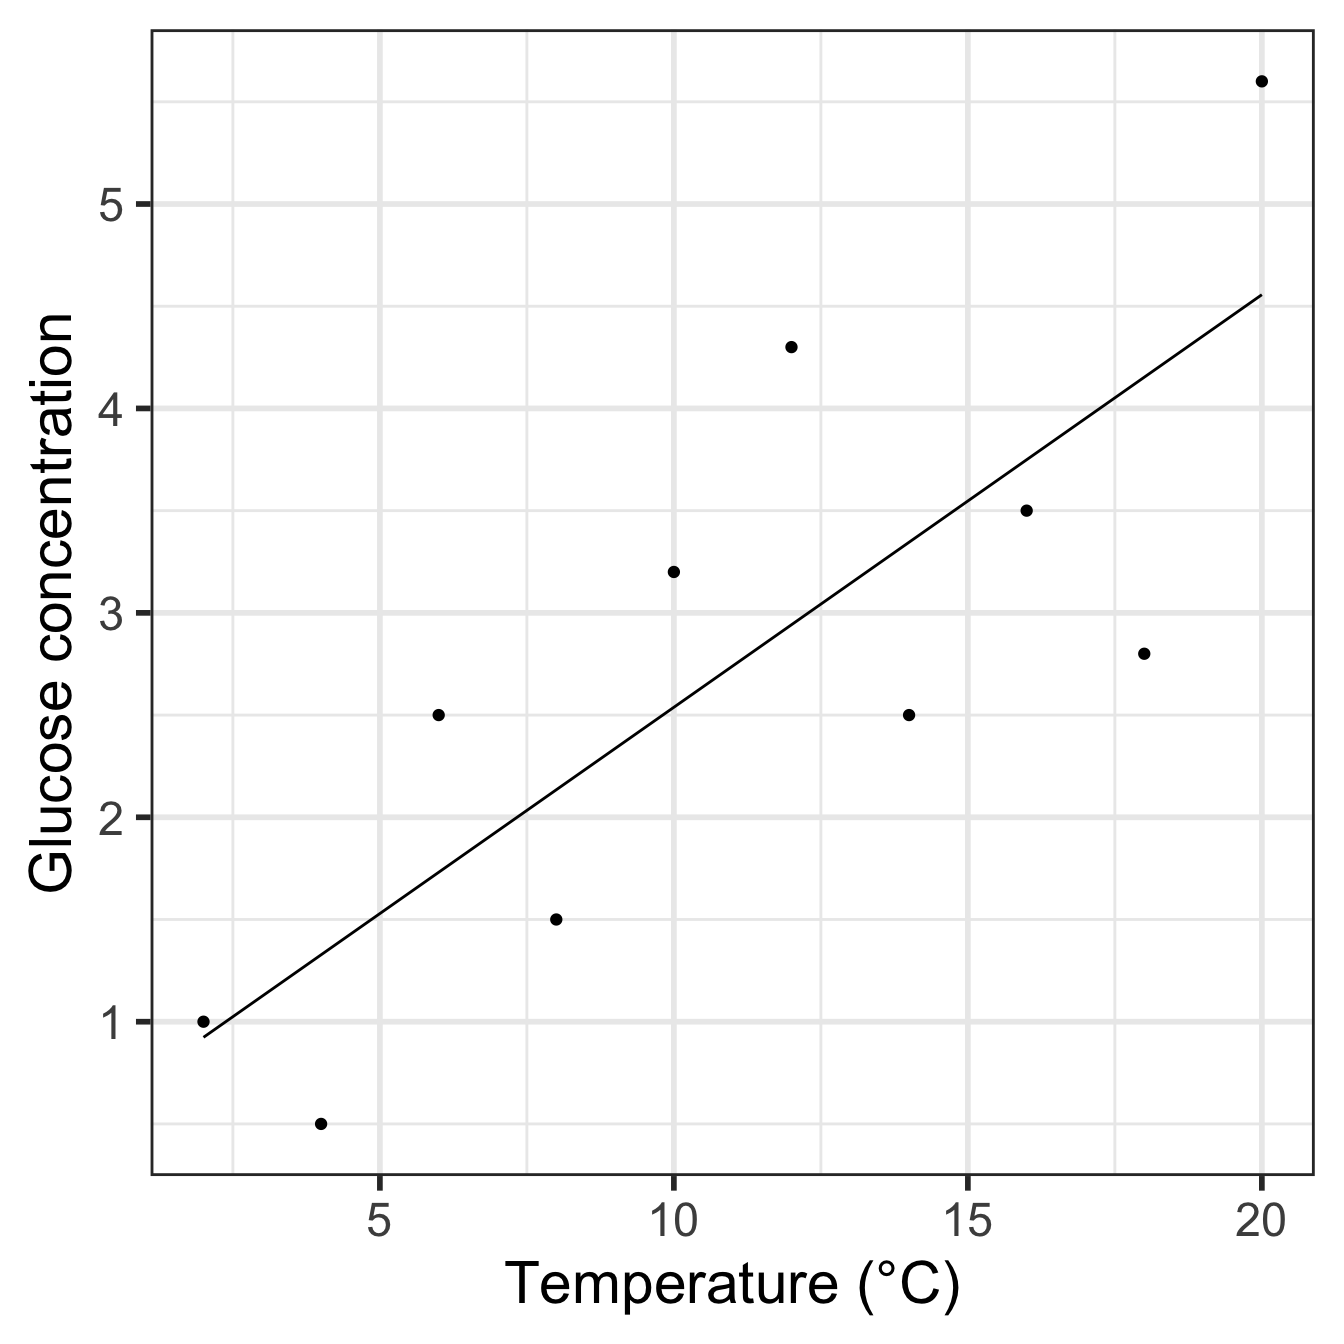
\includegraphics[width=0.6\linewidth]{intro-bio-stats-book_files/figure-latex/reg-worked-publication-1} \end{center}

Notice that we have to make \textbf{ggplot2} use the \texttt{vicia\_germ} data (i.e.~the raw data) when adding the points. We also threw in a little theming to make the plot look nicer.

Here is a quick summary of what we just did:

\begin{itemize}
\tightlist
\item
  Using \texttt{seq} and \texttt{data.frame}, we made a data frame with one column containing the values of the predictor variable we want predictions at.
\item
  We then used the \texttt{predict} function to generate these predictions, adding them to the prediction data with \texttt{mutate}.
\item
  Finally, we used \textbf{ggplot2} to plot the predicted values of the response variable against the predictor variable, remembering to include the data.
\end{itemize}

\hypertarget{regression-causation}{%
\section{What about causation?}\label{regression-causation}}

No discussion of regression would be complete without a little sermon on the fact that just because you observe a (significant) relationship between two variables, this does not necessarily mean that the two variables are causally linked. Suppose we find a negative relationship between the density of oligochaete worms (the response variable) and the density of trout (the predictor variable) in a sample of different streams. In that case, this need not indicate that the trout reduce the numbers of oligochaetes. Oligochaete numbers are often very high in slow-flowing, silty streams where they live in the sediments, whereas trout prefer faster flowing, well-oxygenated, stony streams. A negative correlation could occur simply for that reason. There are many situations in biology where a relationship between two variables can occur, not because there is a causal link between them but because each is related to a third variable (e.g.~habitat).

This difficulty must always be considered when interpreting relationships between variables in data collected from non-experimental situations. However, it is often said that regression analysis can never be used to infer a causal link because of this problem. This is incorrect. What is important is how the data are generated, not the statistical model used to analyse them.

Imagine ten plants were randomly assigned to be grown under ten different light intensities, with all other conditions held constant. In those circumstances it would be entirely proper to analyse the effect of light level on plant height by a regression of plant height (\(y\)) against light level (\(x\)) and, if a significant positive straight-line relationship was found, to conclude that increased light level caused increased plant height. But the fact that we are experimentally producing an effect in plants randomly allocated to each light level is what gives us the confidence to draw a conclusion about causality. Light might not be the direct causal agent---maybe another factor (e.g.~temperature) is varying along with light and causing the effect---but it must be at least indirectly related to plant growth because it was experimentally manipulated.

\hypertarget{part-one-way-anova}{%
\part{One-way ANOVA}\label{part-one-way-anova}}

\hypertarget{introduction-to-one-way-anova}{%
\chapter{Introduction to one-way ANOVA}\label{introduction-to-one-way-anova}}

\hypertarget{intro}{%
\section{Introduction}\label{intro}}

A two-sample \emph{t}-test evaluates whether the mean of a numeric variable changes among two groups. The obvious question is, what happens if we need to compare differences among the means of such a variable measured in more than two groups? It may be tempting to test every pair of means using a two-sample~\emph{t}-test. However, this procedure is statistically flawed. In this chapter, we will introduce a new method to assess the statistical significance of differences among several means simultaneously. This is called~\textbf{Analysis of Variance}~(abbreviated to ANOVA).

ANOVA is one of those statistical terms that unfortunately has two slightly different usages:

\begin{enumerate}
\def\labelenumi{\arabic{enumi}.}
\tightlist
\item
  In its most general sense, ANOVA refers to a methodology for evaluating statistical significance. It often pops up when working with a statistical model known as the `general linear model'. Simple linear regression is one special case of the general linear model\footnote{In fact, whenever we see an \emph{F}-ratio in a statistical test it means we're carrying out an Analysis of Variance of some kind.}.
\item
  In its more narrow sense, the term ANOVA is used to describe a particular type of statistical model. When used like this, ANOVA refers to a class of model used to compare means among two or more groups. The ANOVA-as-a-model is the focus of this chapter.
\end{enumerate}

ANOVA models underpin the analysis of many different kinds of experimental data---they are one of the main `work horses' of data analysis. As with many statistical models, we can use ANOVA without really understanding the details of how it works. However, when interpreting the results of statistical tests associated with ANOVA, it is helpful to have a basic conceptual understanding of how it works. The goal of this chapter is to provide this basic understanding.

We'll do this by exploring the simplest type of ANOVA model: \textbf{One-way Analysis of Variance.} One-way Analysis of Variance allows us to \emph{predict} how the mean value of a numeric variable (the \textbf{response variable}) \emph{responds} or \emph{depends} on the values of a categorical variable (the \textbf{predictor variable}). This statement is just another way of way of saying that the ANOVA model compares means among groups defined by the categorical variable.

It is no coincidence that this sounds a lot like our description of simple regression. ANOVA and regression are both special cases of the general linear model. This observation explains why:

\begin{enumerate}
\def\labelenumi{\arabic{enumi}.}
\tightlist
\item
  regression and ANOVA can be described with a common language (e.g.~response vs predictor variables), and
\item
  the workflows for developing ANOVA and regression analyses are actually very similar in terms of what we have to do in R.
\end{enumerate}

\hypertarget{why-do-we-need-anova-models}{%
\section{Why do we need ANOVA models?}\label{why-do-we-need-anova-models}}

The corncrake, \emph{Crex crex}, underwent severe declines in the UK thought to be due to changes in farming practices. Captive breeding and reintroduction programmes were introduced to try to help supplement the wild population. The scientists in charge of the breeding programme wanted to determine the success of 4 different supplements (the predictor variable) for increasing initial growth (the response variable) in the captive-bred hatchlings. They conducted an experiment in which groups of 8 hatchlings were fed with different supplements. A fifth group of 8 hatchlings served as the control group---they were given the base diet with no supplements. At the end of the experiment, they measured how much weight each hatchling had gained over the week.

We can plot the weight gain of 8 hatchlings on each of the supplements (this is the raw data), along with the means of each supplement group, the standard error of the mean, and the sample mean of all the data (the `global' mean):

\begin{center}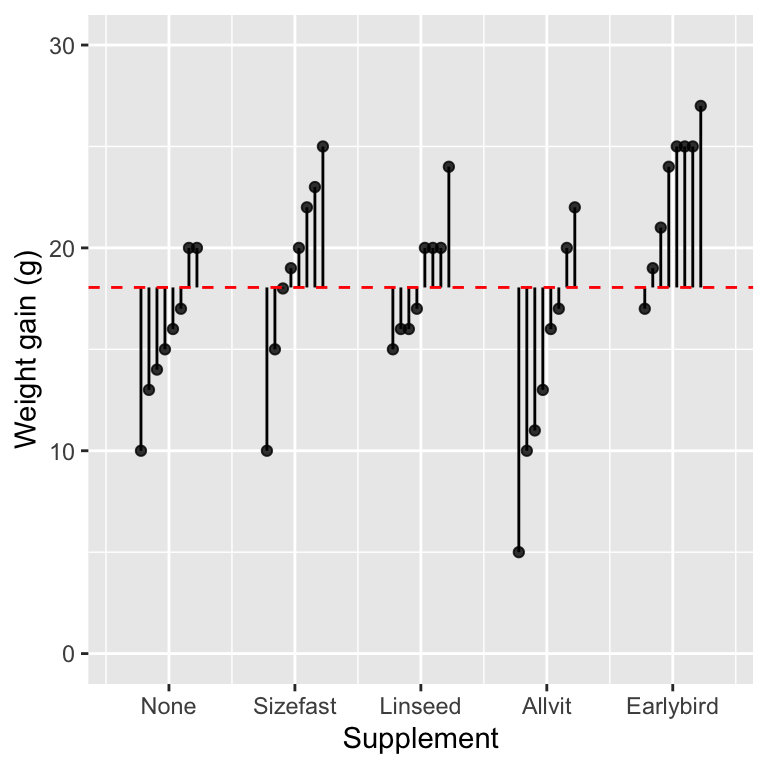
\includegraphics{intro-bio-stats-book_files/figure-latex/unnamed-chunk-95-1} \end{center}

The grey points are the raw data, the means and standard error of each group are in blue, and the overall sample mean is shown by the dashed red line. We can see that there seem to be differences \emph{among} the means: hatchlings in each of the different groups often deviate quite a lot from the global mean (the dashed line). This would seem likely to be an effect of the supplements they are on. At the same time, there is still a lot of variation \emph{within} each group: not all of the hatchlings on the same supplements have the same weight gain.

Perhaps all of this could be explained away as sampling variation---that is, the supplements make no difference at all to weight gain and all we're observing are chance variations. We need a statistical test (or tests) to decide whether these differences are `real'.

It might be tempting to use \emph{t}-tests to compare each mean value with every other mean. This would involve ten \emph{t}-tests on all possible comparisons of the 5 different supplements. Remember, if there is no effect of supplement, then each time we do a \emph{t}-test, there is a chance that we will get a false significant result. Using the conventional \emph{p} = 0.05 significance level, there is a 1 in 20 chance of getting such `false positives'. However, doing several such tests increases the overall risk of finding at least one false positive. In fact, doing ten \emph{t}-tests gives about a 40\% chance of at least one test giving a false positive, even though the individual tests are conducted with \emph{p} = 0.05.

That doesn't sound like a very good way to do science. We need a reliable way to determine whether several means are different or not without increasing the chance of getting a spurious result. That's the job of Analysis of Variance (ANOVA). Just as a two-sample \emph{t}-test compares means between two groups, ANOVA compares means among two \emph{or more} groups. Its name raises an obvious question: if the job of an ANOVA model is to compares means, why is it called Analysis of \emph{Variance}? Let's find out\ldots{}

\hypertarget{how-does-anova-work}{%
\section{How does ANOVA work?}\label{how-does-anova-work}}

The key to understanding ANOVA is to realise that it works by quantifying and comparing different sources of variation in the data. We start with the total variation in the response variable---the variation among all the units in the study---and then partition this into two sources:

\begin{enumerate}
\def\labelenumi{\arabic{enumi}.}
\item
  Variation attributed to the different groups in the data (e.g.~the supplement groups). This is called the `between-group' variation and is equivalent to the `explained variation' described in the regression chapter. It quantifies the variation that is `explained' by the different means. This is the source of variation we usually care about. If this is very low, it means group membership doesn't explain much variation.
\item
  Variation due to other, unmeasured sources. This second source of variation is usually referred to as the `within-group' variation because it applies to experimental units within each group. This quantifies the variation due to everything else that isn't accounted for by the treatments. Within-group variation is also called the `error variation'. We'll mostly use this latter term because it is a bit more general.
\end{enumerate}

ANOVA does compare means, but it does this by looking at changes in variation. That might seem odd, but it works. If the amount of variation among treatments is sufficiently large compared to the within-group variation, this suggests that the treatments are probably having an effect. This means that to understand ANOVA, we have to keep three sources of variation in mind: the total variation, the between-group variation, and the error variation.

We'll get a sense of how this works by carrying on with the corncrake example. We'll look at how to quantify the different sources of variation, and then move on to evaluate statistical significance using these quantities. The thing to keep in mind is that the logic of these calculations is no different from that used to carry out a regression analysis. The only real difference is that we fit means to different groups when working with an ANOVA model instead of fitting a line through the data. Regression and ANOVA both aim to partition (i.e.~split up) the variation in a numeric variable into the parts we can explain and an unexplained leftover part.

\hypertarget{total-variation-1}{%
\subsubsection*{Total variation}\label{total-variation-1}}
\addcontentsline{toc}{subsubsection}{Total variation}

The figure below shows the weight gain of each hatchling in the study and the grand mean (i.e.~we have not plotted the group-specific means).

\begin{center}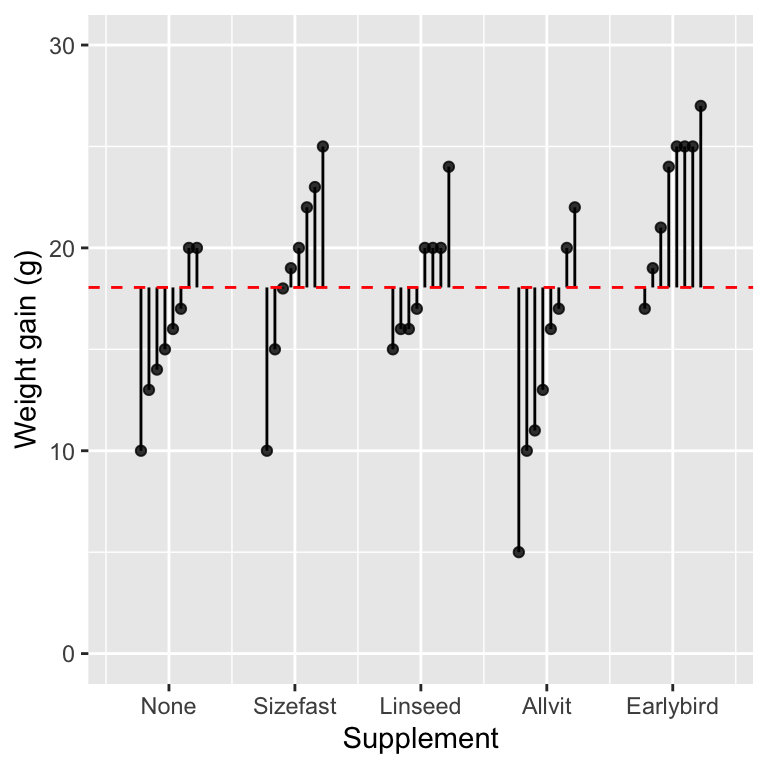
\includegraphics{intro-bio-stats-book_files/figure-latex/unnamed-chunk-98-1} \end{center}

The vertical lines show the distance between each observation and the grand mean---we have ordered the data within each group to make the plot a little tidier. A positive deviation occurs when a point is above the line, and a negative deviation corresponds to a case where the point is below the line. We're not interested in the direction of these deviations. We need to quantify the variability of the deviations. This is a feature of their magnitude (i.e.~the length of the lines).

What measure of variability should we use? We can't add up the deviations because they add to zero. Instead, we apply the same idea introduced in the \protect\hyperlink{relationships-and-regression}{Relationships and regression} chapter: the measure of variability we need is based on the `sum of squares' (abbreviated SS) of the deviations. A sum of squares is calculated by taking each deviation in turn, squaring it, and adding up the squared values. Here are the numeric values of the deviations shown graphically above:

\begin{verbatim}
##  [1]  -5.05   1.95  -1.05  -2.05  -3.05  -4.05  -8.05   1.95  -3.05  -0.05
## [11]  -8.05   3.95   4.95   0.95   6.95   1.95   1.95   5.95  -1.05  -2.05
## [21]   1.95   1.95  -3.05  -2.05   3.95 -13.05  -8.05  -2.05  -7.05  -1.05
## [31]   1.95  -5.05  -1.05   6.95   5.95   6.95   6.95   0.95   8.95   2.95
\end{verbatim}

The sum of squares of these numbers is 967.9. This is called the total sum of squares, because this measure of variability completely ignores the information about treatment groups. It measures the total variability in the response variable, calculated relative to the grand mean.

\hypertarget{residual-variation-1}{%
\subsubsection*{Residual variation}\label{residual-variation-1}}
\addcontentsline{toc}{subsubsection}{Residual variation}

The next component of variability we need relates to the within-group variation. Let's replot the original figure showing the weight gain of each hatchling (points), the mean of each supplement group (horizontal blue lines), and the grand mean:

\begin{center}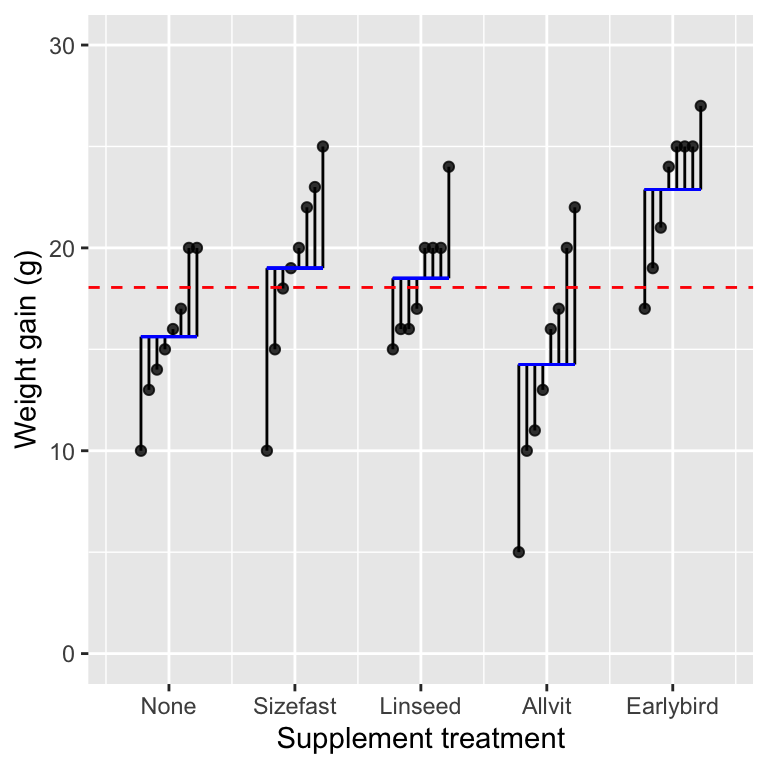
\includegraphics{intro-bio-stats-book_files/figure-latex/unnamed-chunk-100-1} \end{center}

The vertical lines show something new this time. They display the distance between each observation and the group-specific means. They summarise the variation among hatchlings \emph{within} treatment groups. Here are the numeric values of these deviations:

\begin{verbatim}
##  [1] -9.250 -5.625 -9.000 -4.250 -3.250 -2.625 -1.250 -1.625 -0.625 -4.000
## [11] -3.500  0.375 -2.500 -2.500  1.750  1.375 -1.500  2.750 -5.875 -1.000
## [21]  0.000 -3.875  4.375  4.375  1.000  1.500  1.500  1.500  5.750 -1.875
## [31]  3.000  7.750  4.000  5.500  1.125  6.000  2.125  2.125  2.125  4.125
\end{verbatim}

These values are a type of residual: they quantify the `left over' variation after accounting for differences due to treatment groups. Once again, we can summarise this variability as a single number by calculating the associated sum of squares: we take each deviation in turn, square it, and then add up the squared values. The sum of squares of these numbers is (610.25). This is called the residual sum of squares\footnote{You will sometimes see something called error sum of squares, or possibly, the within-group sum of squares. These are just different names for the residual sum of squares.}. It is a measure of the variability that may be attributed to differences among individuals after controlling for the effect of different groups.

\hypertarget{between-group-variation}{%
\subsubsection*{Between-group variation}\label{between-group-variation}}
\addcontentsline{toc}{subsubsection}{Between-group variation}

The last component of variability we need relates to the between group variation. We'll replot the figure one more time, but this time we'll show just the group-specific means (blue points), the overall grand mean (dashed red line), and the deviations of each group mean from the grand mean:

\begin{center}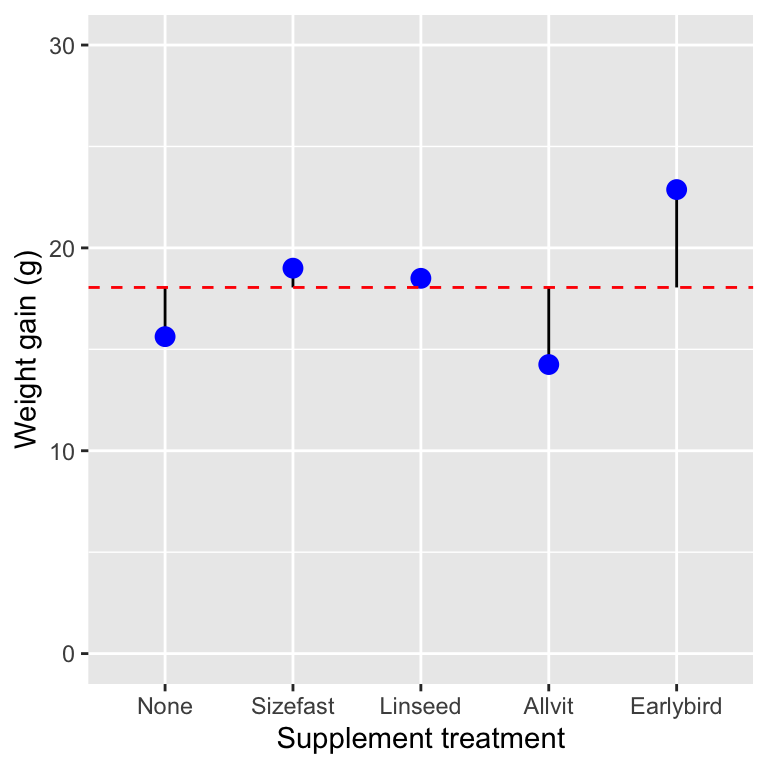
\includegraphics{intro-bio-stats-book_files/figure-latex/unnamed-chunk-102-1} \end{center}

Now the vertical lines show the distance between each group-specific mean and the grand mean. We have five different treatment groups, so there are only five lines. These lines show the variation due to differences among treatment groups. Here are the numeric values of these deviations:

\begin{verbatim}
## [1] -2.425  0.950  0.450 -3.800  4.825
\end{verbatim}

These values quantify the variation that can be attributed to differences among treatments. Once again, we can summarise this variability as a single number by calculating the associated sum of squares---this number is called the treatment sum of squares. This is the same as the `explained sum of squares' discussed in the context of regression. It is a measure of the variability attributed to differences among treatments.

This is 44.71 in the corncrake example. Notice that this is much smaller than the total sum of squares and the residual sum of squares. This isn't all that surprising as it is based on five numbers, whereas the other two measures of variability are based on all the observations.

\hypertarget{degrees-of-freedom}{%
\subsection{Degrees of freedom}\label{degrees-of-freedom}}

The raw sums of squares in ANOVA are a function of sample size and the number of groups. To be useful, we need to convert them into measures of variability that don't scale with the size of a data set. We use \textbf{degrees of freedom} (written as df, or d.f.) to do this. We came across the concept of degrees of freedom when we studied regression: the degrees of freedom associated with a sum of squares quantifies how much `information' it is based on. Each of the three sums of squares we just calculated has a different degrees of freedom calculation associated with it:

\begin{itemize}
\tightlist
\item
  Total d.f. = (Number of observations - 1)
\item
  Treatment d.f. = (Number of treatment groups - 1)
\item
  Error d.f. = (Number of observations - Number of treatment groups)
\end{itemize}

The way to think about these is as follows. We start out with a degrees of freedom equal to the total number of deviations associated with a sum of squares. We then `lose' one degree of freedom for every mean we have to calculate to work out the deviations. Here is how this works in the corncrake example:

\begin{itemize}
\item
  Total d.f. = 40 - 1 = 39 --- The total sum of squares was calculated using all 40 observations in the data, and the deviations were calculated relative to 1 mean (the grand mean).
\item
  Treatment d.f. = 5 - 1 = 4 --- The treatment sum of squares was calculated using the 5 treatment group means, and the deviations were calculated relative to 1 mean (the grand mean).
\item
  Error d.f. = 40 - 5 = 35 --- The error sum of squares was calculated using all 40 observations in the data, and the deviations were calculated relative to 5 means (the treatment group means).
\end{itemize}

Don't worry too much if that seems confusing. We generally don't have to carry out degrees of freedom calculations by hand because R will do them for us. We have reviewed them because knowing where they come from can help understand the output of an ANOVA significance test.

\hypertarget{mean-squares-variance-ratios-and-f-tests}{%
\subsection{Mean squares, variance ratios, and F-tests}\label{mean-squares-variance-ratios-and-f-tests}}

Once we know how to calculate the degrees of freedom, we can use them to standardise each of the sums of squares. The calculations are very simple. We take each sum of squares and divide it by its associated degrees of freedom. The resulting quantity is called a \textbf{mean square} (abbreviated as MS): \[
\text{Mean square} = \frac{\text{Sum of squares}}{\text{Degrees of freedom}}
\] We stated what a mean square represents when discussing regression: it is an estimate of a variance. The mean squares from an ANOVA quantify the variability of the whole sample (total MS), the variability explained by treatment group (treatment MS), and the unexplained residual variation (residual MS).

ANOVA quantifies the strength of the treatment effect by comparing the treatment mean square to the residual mean square. When the treatment MS is large relative to the residual MS, this suggests that the treatments are more likely to be having an effect. In practise, they are compared by calculating the ratio between them (designated by the letter \emph{F}):

\[F = \mbox{Variance ratio} = \frac{\mbox{Variance due to treatments}}{\mbox{Error variance}}\]

This is the equivalent to the \emph{F}-ratio mentioned in the context of regression. When the variation among treatment means (treatment MS) is large compared to the variation due to other factors (residual MS), the~\emph{F}-ratio will be large. If the variation among treatment means is small relative to the residual variation, the~\emph{F}-ratio will be small.

How do we decide when the \emph{F}-ratio is large enough? That is, how do we judge a result to be statistically significant? We play out the usual `gambit':

\begin{enumerate}
\def\labelenumi{\arabic{enumi}.}
\item
  We assume that there is no difference between the population means of each treatment group. That is, we hypothesise that the data in each group were sampled from a single population with one overall global mean.
\item
  Next, we use information in the sample to help us work out what would happen if we were to repeatedly take samples in this hypothetical situation. The `information' in this case corresponds to the mean squares.
\item
  We then ask, `if there is no difference between the groups, what is the probability that we would observe a variance ratio that is the same as, or more extreme than, the one we observed in the real sample?'
\item
  If the observed variance ratio is sufficiently improbable, then we conclude that we have found a `statistically significant' result, i.e.~one that is inconsistent with the hypothesis of no difference.
\end{enumerate}

In order to work through these calculations, we make one key assumption about the population from which the data in each treatment group has been sampled. We assume that the residuals are normally distributed. Once we make this assumption the distribution of the \emph{F}-ratio under the null hypothesis (the `null distribution') has a particular form: it follows an \emph{F} distribution. This means we assess the statistical significance of differences between means by comparing the \emph{F}-ratio calculated from a sample of data to the theoretical \emph{F} distribution.

This procedure is ``methodology for evaluating statistical significance'' we alluded to at the start of this chapter. The resulting \emph{F}-test is no different from the significance testing methodology we outlined for regression models. The important point is that this procedure uses only one comparison---the treatment variation and the error variation---rather than the ten individual \emph{t}-tests that would have been required to compare all the pairs.

One thing to be aware of is that the \emph{F}-tests are typically global tests of significance: they indicate whether groups are different but don't tell us anything about which groups might be driving a significant result. That kind of question needs another test. We will examine one such test in the multiple comparison chapter later.

\hypertarget{different-kinds-of-anova-model}{%
\section{Different kinds of ANOVA model}\label{different-kinds-of-anova-model}}

There are many different flavours of ANOVA model. The one we've just been learning about is called a one-way ANOVA. It's called one-way ANOVA because it involves only one factor: supplement type (this includes the control). If we had considered two factors---e.g.~supplement type and amount of food---we would have to use something called a two-way ANOVA. A design with three factors is called a three-way ANOVA, and\ldots{} you get the idea.

There are many other ANOVA models, each of which is used to analyse a specific type of experimental design. We will only consider three different types of ANOVA in this book: one-way ANOVA, two-way ANOVA, and ANOVA for one-way, blocked design experiments.

\hypertarget{questions}{%
\section{Some common questions about ANOVA}\label{questions}}

To finish off with, three common questions that often arise:

\hypertarget{can-anova-only-be-applied-to-experimental-data}{%
\subsection{Can ANOVA only be applied to experimental data?}\label{can-anova-only-be-applied-to-experimental-data}}

We have been discussing ANOVA in the context of a designed experiment (i.e.~we talked about treatments and control groups). Although ANOVA was developed to analyse experimental data, which is where it is most powerful, it can be used in an observational setting. As long as we're careful about how we sample different groups, we can use ANOVA to analyse their differences. The main difference between ANOVA for experimental and observational studies arises in the interpretation of the results. If the data aren't experimental, we can't say anything concrete about the causal nature of observed among-group differences.

\hypertarget{do-we-need-equal-replication}{%
\subsection{Do we need equal replication?}\label{do-we-need-equal-replication}}

One of the frequent problems with biological data is we often don't have equal replication. Even if we started with equal replication in our design, all sorts of things conspire to upset even the best-designed experiments. For example, plants and animals have a habit of dying before we have gathered all our data: a pot may get dropped or a culture contaminated. Does this matter? Not really. One-way ANOVA does not require equal replication and will work just fine where sample sizes differ between treatments.

\hypertarget{can-anova-be-done-with-only-two-treatments}{%
\subsection{Can ANOVA be done with only two treatments?}\label{can-anova-be-done-with-only-two-treatments}}

Although the~\emph{t}-test provides a convenient way of testing means from two treatments, nothing stops you from doing an ANOVA on two treatments. A~\emph{t}-test (assuming equal variances) and ANOVA on the same data should give the same~\emph{p}-value (in fact, the~\emph{F}-statistic from the ANOVA will be the square of the~\emph{t}-value from the~\emph{t}-test). However, one advantage to the~\emph{t}-test is that you can do the version of the test that allows for unequal variances---something a standard ANOVA does not do. There is a version of Welch's test for one-way ANOVA, but we won't study it in this book (look at the \texttt{oneway.test} function if you are interested).

\hypertarget{one-way-anova-in-R}{%
\chapter{One-way ANOVA in R}\label{one-way-anova-in-R}}

Our goal in this chapter is to learn how to work with one-way ANOVA models in R. As we did with regression, we'll do this by working through an example. We'll start with the problem and the data, then work through model fitting, significance testing, and finally, present the results.

\hypertarget{introduction-3}{%
\section{Introduction}\label{introduction-3}}

We will use the corncrake example from the last chapter to demonstrate how to conduct a one-way ANOVA in R. Recall that these data show the results of an experiment comparing the weight gain of eight corncrake hatchlings on each of four supplements and one control diet.

\begin{infobox}{action}

\hypertarget{section-8}{%
\subsubsection*{}\label{section-8}}
\addcontentsline{toc}{subsubsection}{}

The data live in the `CORN\_CRAKE.CSV' file. The code below assumes those data have been read into a tibble called \texttt{corn\_crake}. Set that up if you plan to work along.

\end{infobox}

\hypertarget{first-steps-1}{%
\subsection{First steps}\label{first-steps-1}}

What lives inside the \texttt{corn\_crake} data set? There are no surprises:

\begin{Shaded}
\begin{Highlighting}[]
\FunctionTok{glimpse}\NormalTok{(corn\_crake)}
\end{Highlighting}
\end{Shaded}

\begin{verbatim}
## Rows: 40
## Columns: 2
## $ Supplement <chr> "None", "None", "None", "None", "None", "None", "None", "No~
## $ WeightGain <dbl> 13, 20, 17, 16, 15, 14, 10, 20, 15, 18, 10, 22, 23, 19, 25,~
\end{verbatim}

There are 40 observations in the data set and 2 variables (columns), called \texttt{Supplement} and \texttt{WeightGain}.

\hypertarget{visualising-the-data-1}{%
\subsection{Visualising the data}\label{visualising-the-data-1}}

We should plot our data before we even consider fitting a model. One way to do this is by creating a boxplot:

\begin{Shaded}
\begin{Highlighting}[]
\FunctionTok{ggplot}\NormalTok{(corn\_crake, }\FunctionTok{aes}\NormalTok{(}\AttributeTok{x =}\NormalTok{ Supplement, }\AttributeTok{y =}\NormalTok{ WeightGain)) }\SpecialCharTok{+} 
  \FunctionTok{geom\_boxplot}\NormalTok{()}
\end{Highlighting}
\end{Shaded}

\begin{center}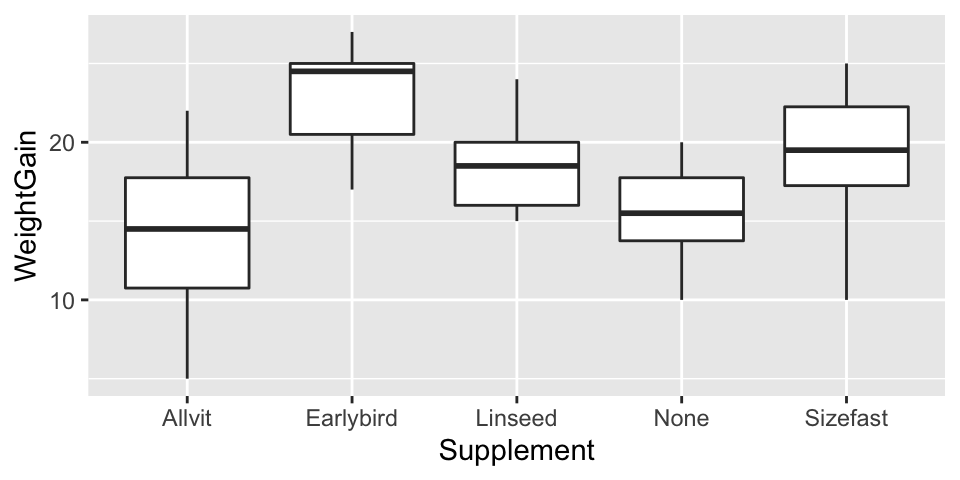
\includegraphics{intro-bio-stats-book_files/figure-latex/unnamed-chunk-107-1} \end{center}

At this point, we just want to get an idea of what our data look like. We don't need to worry about customising the plot to make it look nice.

\begin{infobox}{action}

\hypertarget{examine-the-plot}{%
\subsubsection*{Examine the plot}\label{examine-the-plot}}
\addcontentsline{toc}{subsubsection}{Examine the plot}

Have a look at the plot and think about what it means biologically. Which supplement seems to have had the biggest effect? Do all of the supplements increase growth relative to the control?

\end{infobox}

\hypertarget{model-fitting-and-significance-tests-1}{%
\section{Model fitting and significance tests}\label{model-fitting-and-significance-tests-1}}

Carrying out ANOVA in R is quite simple, but as with regression, there is more than one step.

The first involves a process known as \emph{fitting the model} (or just \emph{model fitting}). This is the step where R calculates the relevant means and the additional information needed to generate the results in step two. We call this step model fitting because an ANOVA is a type of model for our data: it is a model that allows the mean of a variable to vary among groups.

How do we fit an ANOVA model in R? We use the \texttt{lm} function again. Remember what the letters `lm' stand for? They stand for `(general) linear model'. An ANOVA model is just another special case of that general linear model. Here is how we fit a one-way ANOVA in R, using the corncrake data:

\begin{Shaded}
\begin{Highlighting}[]
\NormalTok{corncrake\_model }\OtherTok{\textless{}{-}} \FunctionTok{lm}\NormalTok{(WeightGain }\SpecialCharTok{\textasciitilde{}}\NormalTok{ Supplement, }\AttributeTok{data =}\NormalTok{ corn\_crake)}
\end{Highlighting}
\end{Shaded}

By now, this kind of thing is probably starting to look familiar. We have to assign two arguments:

\begin{enumerate}
\def\labelenumi{\arabic{enumi}.}
\item
  The first argument is a formula. We know this because it includes a `tilde' symbol: \texttt{\textasciitilde{}}. The variable name on the left of the \texttt{\textasciitilde{}} must be the numeric response variable whose means we want to compare among groups. The variable on the right should be the indicator (or predictor) variable that says which group each observation belongs to. These are \texttt{WeightGain} and \texttt{Supplement}, respectively.
\item
  The second argument is the name of the data frame that contains the two variables listed in the formula.
\end{enumerate}

\begin{infobox}{information}

\hypertarget{how-does-r-know-which-model-to-use}{%
\subsubsection*{How does R know which model to use?}\label{how-does-r-know-which-model-to-use}}
\addcontentsline{toc}{subsubsection}{How does R know which model to use?}

How does R know we want to use an ANOVA model? After all, we didn't specify this anywhere. The answer is that R looks at what type of vector \texttt{Supplement} is. It is a categorical character vector, and so R carries out an ANOVA. It would do the same if \texttt{Supplement} had been a factor. However, if the values of \texttt{Supplement} had been stored as numbers then R would not have fitted an ANOVA. Instead, it would have assumed we meant to fit a regression model, which is seldom appropriate. \textbf{This is why we never store categorical variables as numbers in R.}

Avoid using numbers to encode the values of a categorical variable if you want to avoid making mistakes when fitting models!

\end{infobox}

Notice that we did not print the results to the console. Instead, we assigned the result a name ---\texttt{corncrake\_model} now refers to a \textbf{model object}. What happens if we print this to the console?

\begin{Shaded}
\begin{Highlighting}[]
\NormalTok{corncrake\_model}
\end{Highlighting}
\end{Shaded}

\begin{verbatim}
## 
## Call:
## lm(formula = WeightGain ~ Supplement, data = corn_crake)
## 
## Coefficients:
##         (Intercept)  SupplementEarlybird    SupplementLinseed  
##              14.250                8.625                4.250  
##      SupplementNone   SupplementSizefast  
##               1.375                4.750
\end{verbatim}

Not a great deal. Printing a fitted model object to the console is not very useful when working with ANOVA. We just see a summary of the model we fitted and some information about the model coefficients. Yes, an ANOVA model has coefficients, just like a regression does.

\begin{infobox}{warning}

\hypertarget{assumptions-1}{%
\subsubsection*{Assumptions}\label{assumptions-1}}
\addcontentsline{toc}{subsubsection}{Assumptions}

The one-way ANOVA model has a series of assumptions about how the data are generated. This point in the workflow would be a good place to evaluate whether or not these may have been violated. However, we're going to tackle this later in the \protect\hyperlink{assumptions-diagnostics}{Assumptions} and \protect\hyperlink{regression-diagnostics}{Diagnostics} chapters. For now, it is enough to be aware that there are assumptions associated with one-way ANOVA and that you should evaluate these when working with your own data.

\end{infobox}

\hypertarget{interpreting-the-results}{%
\subsection{Interpreting the results}\label{interpreting-the-results}}

We really want a~\emph{p}-value to help us determine whether there is statistical support for a difference among the group means. That is, we need to calculate things like degrees of freedom, sums of squares, mean squares, and the \emph{F}-ratio. This is step 2.

We use the \texttt{anova} function to do this:

\begin{Shaded}
\begin{Highlighting}[]
\FunctionTok{anova}\NormalTok{(corncrake\_model)}
\end{Highlighting}
\end{Shaded}

\begin{verbatim}
## Analysis of Variance Table
## 
## Response: WeightGain
##            Df Sum Sq Mean Sq F value   Pr(>F)   
## Supplement  4 357.65  89.413  5.1281 0.002331 **
## Residuals  35 610.25  17.436                    
## ---
## Signif. codes:  0 '***' 0.001 '**' 0.01 '*' 0.05 '.' 0.1 ' ' 1
\end{verbatim}

Notice that all we did was pass the \texttt{anova} function one argument: the name of the fitted model object. Let's step through the output to see what it means. The first line just informs us that we are looking at an ANOVA table, i.e.~a table of statistical results from an analysis of variance. The second line just reminds us of what variable we analysed.

The important information is in the table that follows:

\begin{verbatim}
##            Df Sum Sq Mean Sq F value   Pr(>F)    
## Supplement  4 357.65  89.413  5.1281 0.002331 ** 
## Residuals  35 610.25  17.436
\end{verbatim}

This is an Analysis of Variance Table. It summarises the parts of the ANOVA calculation: \texttt{Df} -- degrees of freedom, \texttt{Sum\ Sq} -- the sum of squares, \texttt{Mean\ Sq} -- the mean square, \texttt{F\ value} -- the \emph{F}-ratio (i.e.~variance ratio), \texttt{Pr(\textgreater{}F)} -- the \emph{p}-value.

The \emph{F}-ratio (variance ratio) is the key term. This is the test statistic. It measures how large and consistent the differences between the means of the five different treatments are. Larger values indicate clearer differences between means, in just the same way that large values of Student's \emph{t} indicate clearer differences between means in the two sample situation.

The \emph{p}-value gives the probability that the observed differences between the means, or a more extreme difference, could have arisen through sampling variation under the null hypothesis. What is the null hypothesis: it is one of no effect of treatment, i.e.~the null hypothesis is that all the means are the same. As always, the \emph{p}-value of 0.05 is used as the significance threshold, and we take \emph{p} \textless{} 0.05 as evidence that at least one of the treatments is having an effect. For the corncrake data, the value is 5.1, and the probability (\emph{p}) of getting an \emph{F}-ratio this large is given by R as 0.0023, i.e.~less than 0.05. This provides good evidence that there are differences in weight gain between at least some of the treatments.

So far so good. The test that we have just carried out is called the \textbf{global test of significance}. It goes by this name because it doesn't tell us anything about which means are different. The analyses suggest that there is an effect of supplement on weight gain. Still, some uncertainty remains because we have only established that there are differences among at least some supplements. A global test doesn't say which supplements are better or worse. This could be very important. If the significant result is generated by all supplements being equally effective (hence differing from the control but not from each other) we would draw very different conclusions than if the result was a consequence of one supplement being very effective and all the others being useless. Our result could even be produced by the supplements all being less effective than the control!

So having got a significant result in the ANOVA, we should always look at the means of the treatments to understand where the differences actually lie. We did this in the previous chapter but here is the figure again anyway:

\begin{center}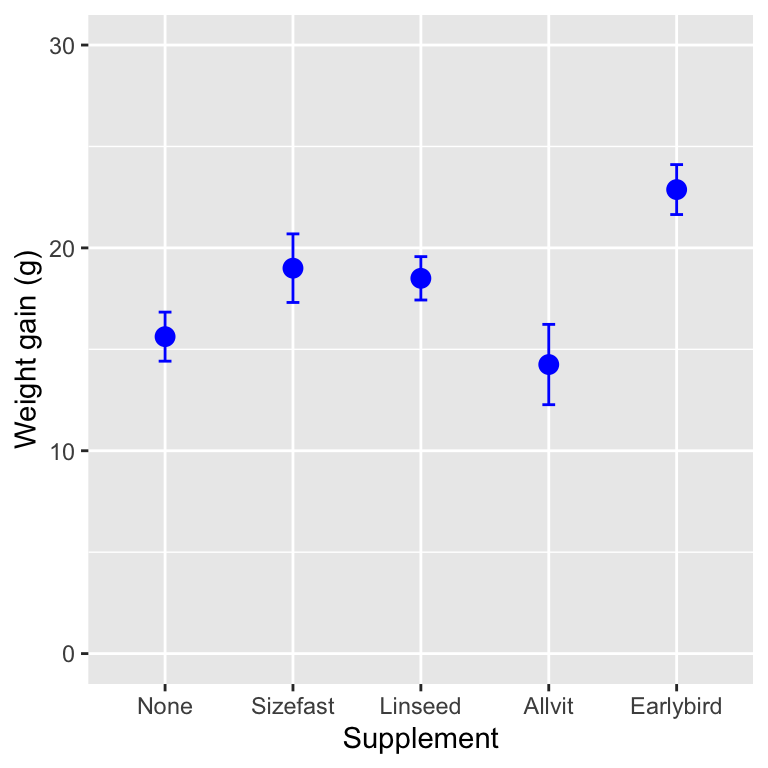
\includegraphics{intro-bio-stats-book_files/figure-latex/diet-summary-all-1} \end{center}

What looking at the means tells us is that the effect of the supplements is generally to increase weight gain (with one exception, `Allvit') relative to the control group (`None'), and that it looks as though `Earlybird' is the most effective, followed by `Sizefast' and `Linseed'.

Often inspection of the means in this way will tell us all we need to know and no further work will be required. However, sometimes it is desirable to have a more rigorous way of testing where the significant differences between treatments occur. A number of tests exist as `add ons' to ANOVA which enable you to do this. These are called \textbf{post hoc multiple comparison tests} (sometimes just `multiple comparison tests'). We'll see how to conduct these later.

\hypertarget{summarise-results-anova}{%
\section{Presenting results}\label{summarise-results-anova}}

As with all tests, it will be necessary to summarise the result in a written form. With an ANOVA on several treatments, we always need to at least summarise the result of the global test of significance, for example:

\begin{quote}
There was a significant effect of supplement on the weight gain of the corncrake hatchlings (ANOVA: F=5.1; d.f.= 4,35; p\textless0.01).
\end{quote}

There are several things to notice here:

\begin{itemize}
\item
  The degrees of freedom are always quoted as part of the result, and\ldots there are \emph{two values for the degrees of freedom} to report in ANOVA because it involves \emph{F}-ratios. These are obtained from the ANOVA table and should be given as the treatment degrees of freedom first, followed by the error degrees of freedom. Order matters. Don't mix it up.
\item
  The degrees of freedom are important because, like a \emph{t}-statistic, the significance of an \emph{F}-ratio depends on the degrees of freedom, and giving them helps the reader to judge the result you are presenting. A large value may not be very significant if the sample size is small, a smaller may be highly significant if the sample sizes are large.
\item
  The \emph{F}-ratio rarely needs to be quoted to more than one decimal place.
\end{itemize}

When it comes to presenting the results in a report, it helps to present the means, as the statement above cannot entirely capture the results. We could use a table to do this, but tables are ugly and difficult to interpret. A good figure is much better.

Box and whiskers plots and multi-panel dot plots or histograms are exploratory data analysis tools. We use them at the beginning of an analysis to understand the data, but we don't tend to present them in project reports or scientific papers. Since ANOVA is designed to compare means, a minimal plot needs to show the point estimates of each group-specific mean, along with a measure of their uncertainty. We often use the standard error of the means to summarise this uncertainty.

In order to be able to plot these quantities we first have to calculate them. We can do this using \texttt{dplyr}. Here's a reminder of the equation for the standard error of a mean: \[
SE = \frac{\text{Standard deviation of the sample}}{\sqrt{\text{Sample size}}} = \frac{SD}{\sqrt{n}}
\] So, the required \texttt{dplyr} code is:

\begin{Shaded}
\begin{Highlighting}[]
\CommentTok{\# get the mean and the SE for each supplement}
\NormalTok{corncrake\_stats }\OtherTok{\textless{}{-}} 
\NormalTok{  corn\_crake }\SpecialCharTok{\%\textgreater{}\%} 
  \FunctionTok{group\_by}\NormalTok{(Supplement) }\SpecialCharTok{\%\textgreater{}\%} 
  \FunctionTok{summarise}\NormalTok{(}\AttributeTok{Mean =} \FunctionTok{mean}\NormalTok{(WeightGain), }\AttributeTok{SE =} \FunctionTok{sd}\NormalTok{(WeightGain)}\SpecialCharTok{/}\FunctionTok{sqrt}\NormalTok{(}\FunctionTok{n}\NormalTok{()))}
\CommentTok{\# print to the console}
\NormalTok{corncrake\_stats}
\end{Highlighting}
\end{Shaded}

\begin{verbatim}
## # A tibble: 5 x 3
##   Supplement  Mean    SE
##   <chr>      <dbl> <dbl>
## 1 Allvit      14.2  1.98
## 2 Earlybird   22.9  1.23
## 3 Linseed     18.5  1.07
## 4 None        15.6  1.21
## 5 Sizefast    19    1.69
\end{verbatim}

Notice that we used the \texttt{n} function to get the sample size. The rest of this R code should be quite familiar by now. We gave the data frame containing the group-specific means and standard errors the name \texttt{corncrake\_stats}.

We have a couple of different options for making a good summary figure. The first plots a point for each mean and places error bars around this to show ±1 SE. In order to do this using \texttt{ggplot2} we have to add \emph{two layers}---the first specifies the points (the means) and the second specifies the error bar (the SE). Here is how to do this:

\begin{Shaded}
\begin{Highlighting}[]
\FunctionTok{ggplot}\NormalTok{(}\AttributeTok{data =}\NormalTok{ corncrake\_stats, }
       \FunctionTok{aes}\NormalTok{(}\AttributeTok{x =}\NormalTok{ Supplement, }\AttributeTok{y =}\NormalTok{ Mean, }\AttributeTok{ymin =}\NormalTok{ Mean }\SpecialCharTok{{-}}\NormalTok{ SE, }\AttributeTok{ymax =}\NormalTok{ Mean }\SpecialCharTok{+}\NormalTok{ SE)) }\SpecialCharTok{+} 
  \CommentTok{\# this adds the means}
  \FunctionTok{geom\_point}\NormalTok{(}\AttributeTok{colour =} \StringTok{"blue"}\NormalTok{, }\AttributeTok{size =} \DecValTok{3}\NormalTok{) }\SpecialCharTok{+} 
  \CommentTok{\# this adds the error bars}
  \FunctionTok{geom\_errorbar}\NormalTok{(}\AttributeTok{width =} \FloatTok{0.1}\NormalTok{, }\AttributeTok{colour =} \StringTok{"blue"}\NormalTok{) }\SpecialCharTok{+} 
  \CommentTok{\# controlling the appearance}
  \FunctionTok{scale\_y\_continuous}\NormalTok{(}\AttributeTok{limits =} \FunctionTok{c}\NormalTok{(}\DecValTok{0}\NormalTok{, }\DecValTok{30}\NormalTok{)) }\SpecialCharTok{+} 
  \CommentTok{\# use sensible labels}
  \FunctionTok{xlab}\NormalTok{(}\StringTok{"Supplement treatment"}\NormalTok{) }\SpecialCharTok{+} \FunctionTok{ylab}\NormalTok{(}\StringTok{"Weight gain (g)"}\NormalTok{) }\SpecialCharTok{+}
  \CommentTok{\# flip x and y axes}
  \FunctionTok{coord\_flip}\NormalTok{() }\SpecialCharTok{+}
  \CommentTok{\# use a more professional theme}
  \FunctionTok{theme\_bw}\NormalTok{()}
\end{Highlighting}
\end{Shaded}

\begin{center}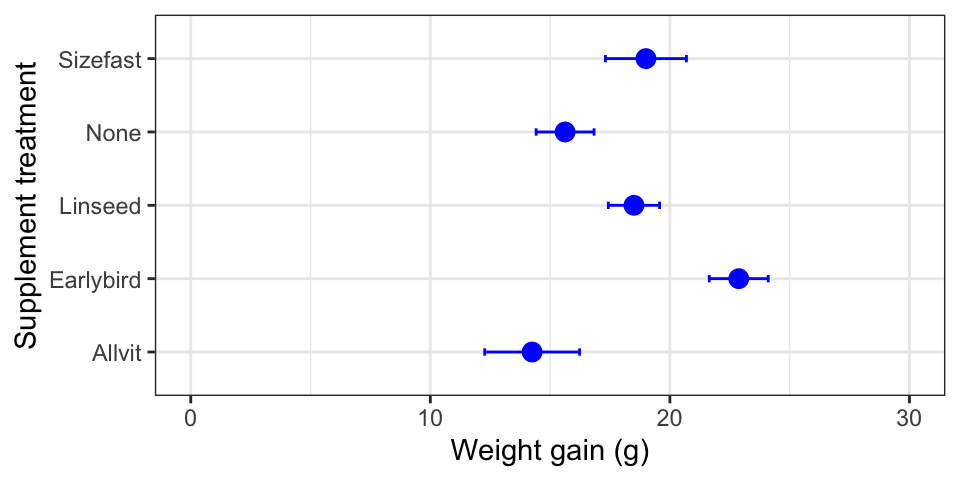
\includegraphics{intro-bio-stats-book_files/figure-latex/diet-summary-initial-1} \end{center}

First, notice that we set the \texttt{data} argument in \texttt{ggplot} to be the data frame containing the summary statistics (not the original raw data). Second, we set up four aesthetic mappings: \texttt{x}, \texttt{y}, \texttt{ymin} and \texttt{ymax}. Third, we added one layer using \texttt{geom\_point}. This adds the individual points based on the \texttt{x} and \texttt{y} mappings. Fourth, we added a second layer using \texttt{geom\_errorbar}. This adds the error bars based on the \texttt{x}, \texttt{ymin} and \texttt{ymax} mappings. Finally we adjusted the y limits and the labels (this last step is optional). Ask a demonstrator to step through this with you if you are confused by it.

\begin{infobox}{information}

\hypertarget{factors}{%
\subsubsection*{Factors}\label{factors}}
\addcontentsline{toc}{subsubsection}{Factors}

Now is good time to take a short detour to remind ourselves about factors. In the world of experimental design, the word `factor' is used to describe a controlled variable where the levels---i.e.~its different values or categories---are set by the experimenter. R includes a special type of vector for representing factors. This is called, rather sensibly, a factor. One can get quite a long way in R-land without using factors. However, we inevitably end up using them because so much of R's plotting and statistical modelling machinery rely on factors. We are going to need to them to help us reorder the groups in our plot.

\end{infobox}

Take a close look at that last figure. Is there anything wrong with it? The control group in this study is the no diet group (`None'). Conventionally, we display the control groups first. R hasn't done this because the different categories of \texttt{Supplement} are presented in alphabetical order by default. One way to change that order if by converting \texttt{Supplement} to a factor and define the order we want as we do so. Here is how to do this using \texttt{dplyr} and a function called \texttt{factor}:

\begin{Shaded}
\begin{Highlighting}[]
\NormalTok{corncrake\_stats }\OtherTok{\textless{}{-}} 
\NormalTok{  corncrake\_stats }\SpecialCharTok{\%\textgreater{}\%} 
  \FunctionTok{mutate}\NormalTok{(}\AttributeTok{Supplement =} \FunctionTok{factor}\NormalTok{(Supplement, }
                             \AttributeTok{levels =} \FunctionTok{c}\NormalTok{(}\StringTok{"None"}\NormalTok{, }\StringTok{"Sizefast"}\NormalTok{, }\StringTok{"Linseed"}\NormalTok{, }\StringTok{"Allvit"}\NormalTok{, }\StringTok{"Earlybird"}\NormalTok{)))}
\end{Highlighting}
\end{Shaded}

We use \texttt{mutate} to update \texttt{Supplement}, using the \texttt{factor} function to redefine the levels of \texttt{Supplement} and overwrite the original. Now, when we rerun the \texttt{ggplot2} code we end up with a figure like this:

\begin{center}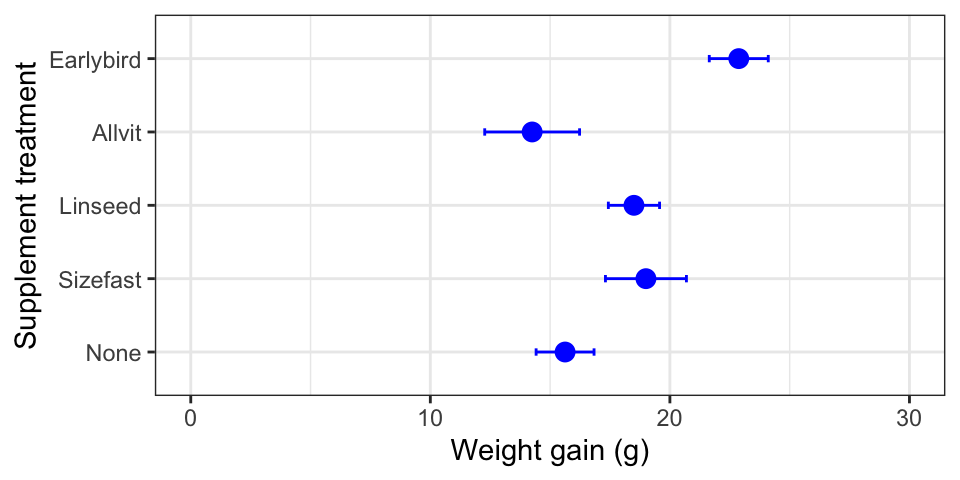
\includegraphics{intro-bio-stats-book_files/figure-latex/diet-summary-releveled-1} \end{center}

The treatments are presented in the order specified with the \texttt{levels} argument. Problem solved!

A bar plot is another popular visualisation for summarising the results of an ANOVA. We only have to change one thing about the last chunk of \texttt{ggplot2} code to make a bar plot. Instead of using \texttt{geom\_point}, we use \texttt{geom\_col} (we'll drop the \texttt{coord\_flip} bit too):

\begin{Shaded}
\begin{Highlighting}[]
\FunctionTok{ggplot}\NormalTok{(}\AttributeTok{data =}\NormalTok{ corncrake\_stats, }
       \FunctionTok{aes}\NormalTok{(}\AttributeTok{x =}\NormalTok{ Supplement, }\AttributeTok{y =}\NormalTok{ Mean, }\AttributeTok{ymin =}\NormalTok{ Mean }\SpecialCharTok{{-}}\NormalTok{ SE, }\AttributeTok{ymax =}\NormalTok{ Mean }\SpecialCharTok{+}\NormalTok{ SE)) }\SpecialCharTok{+} 
  \CommentTok{\# this adds the means}
  \FunctionTok{geom\_col}\NormalTok{(}\AttributeTok{fill =} \StringTok{"lightgrey"}\NormalTok{, }\AttributeTok{colour =} \StringTok{"grey"}\NormalTok{) }\SpecialCharTok{+} 
  \CommentTok{\# this adds the error bars}
  \FunctionTok{geom\_errorbar}\NormalTok{(}\AttributeTok{width =} \FloatTok{0.1}\NormalTok{, }\AttributeTok{colour =} \StringTok{"black"}\NormalTok{) }\SpecialCharTok{+} 
  \CommentTok{\# controlling the appearance}
  \FunctionTok{scale\_y\_continuous}\NormalTok{(}\AttributeTok{limits =} \FunctionTok{c}\NormalTok{(}\DecValTok{0}\NormalTok{, }\DecValTok{30}\NormalTok{)) }\SpecialCharTok{+} 
  \CommentTok{\# use sensible labels}
  \FunctionTok{xlab}\NormalTok{(}\StringTok{"Supplement treatment"}\NormalTok{) }\SpecialCharTok{+} \FunctionTok{ylab}\NormalTok{(}\StringTok{"Weight gain (g)"}\NormalTok{) }\SpecialCharTok{+} 
  \CommentTok{\# use a more professional theme}
  \FunctionTok{theme\_bw}\NormalTok{()}
\end{Highlighting}
\end{Shaded}

\begin{center}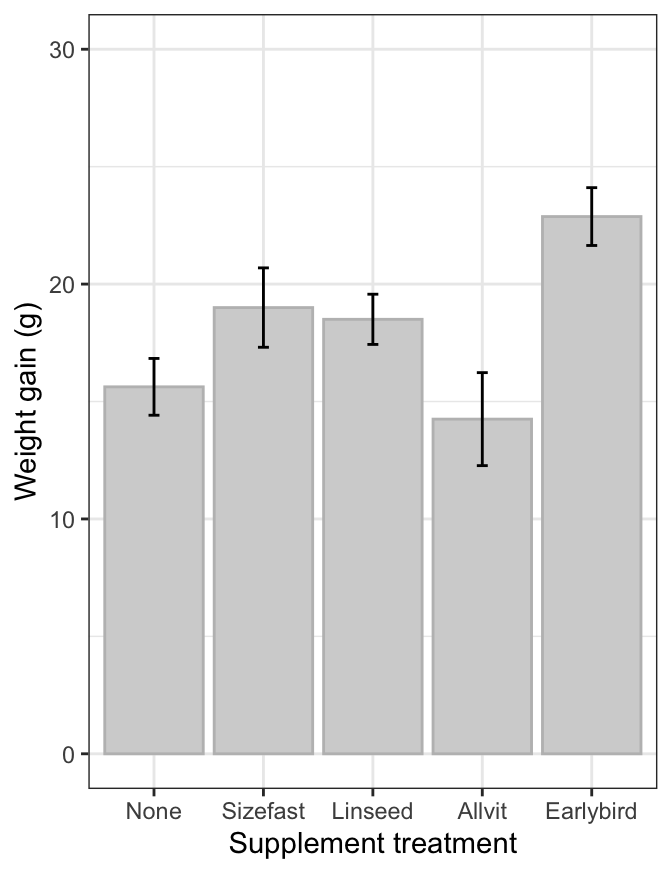
\includegraphics{intro-bio-stats-book_files/figure-latex/diet-summary-points-1} \end{center}

\hypertarget{multiple-comparison-tests-chapter}{%
\chapter{Multiple comparison tests}\label{multiple-comparison-tests-chapter}}

In the \protect\hyperlink{one-way-anova-in-R}{One-way ANOVA in R} chapter, we learned how to examine the global hypothesis of no difference between means. That test does not evaluate \emph{which} means might be driving a significant result. For example, in the corncrake example, we found evidence of a significant effect of dietary supplement on the mean hatchling growth rate. However, our analysis did not tell us which supplements are better or worse and did not make any statements about which supplements differ significantly from each other. The purpose of this chapter is to examine one method for assessing where the differences lie.

\hypertarget{post-hoc-multiple-comparisons-tests}{%
\section{Post hoc multiple comparisons tests}\label{post-hoc-multiple-comparisons-tests}}

The general method we will use is called a \textbf{post hoc multiple comparisons test}. The phrase `post hoc' refers to the fact that these tests are conducted without any particular prior comparisons in mind. The words `multiple comparisons' refer to the fact that they consider many different pairwise comparisons. There are quite a few multiple comparison tests---Scheffé's test, the Student-Newman-Keuls test, Duncan's new multiple range test, Dunnett's test, \ldots{} (the list goes on and on). Each one applies to particular circumstances, and none is universally accepted as `the best'. We are going to work with the most widely used test: the \textbf{Tukey multiple comparison test}. This test is also known as Tukey's Honestly Significant Difference (Tukey HSD) test\footnote{N.B. Try to avoid a common mistake: it is \emph{Tukey}, after its originator, the statistician Prof.~John Tukey, not Turkey, a large domesticated bird which has made no useful contributions to statistical theory or practice.}.

People tend to favour Tukey's HSD test because it is `conservative': the test has a low false-positive rate compared to the alternatives. A false positive occurs when a test turns up a statistically significant result for an effect that is not there. A low false-positive rate is a good thing. It means that if we find a significant difference, we can be more confident it is `real'. The cost of using the Tukey HSD test is that it isn't as powerful as alternatives: the test turns up a lot of false negatives. A false negative occurs when a test fails to produce a statistically significant result for an effect when it is present. A test with a high false-negative rate tends to miss effects.

One line of thinking says post hoc multiple comparisons tests of any kind should never be undertaken. We shouldn't carry out an experiment without a prior prediction of what will happen---we should know which comparisons need to be made and should only undertake those particular comparisons rather than making every possible comparison. Nonetheless, post hoc multiple comparisons tests are easy to apply and widely used, so there is value in knowing how to use them. The Tukey HSD test at least tends to guard against picking up non-existent effects.

\hypertarget{mult-comp-R}{%
\section{Tukey's HSD test in R}\label{mult-comp-R}}

We will use the corncrake example to illustrate how to use R to carry out and interpret Tukey's HSD test.

\begin{infobox}{action}

\hypertarget{section-9}{%
\subsubsection*{}\label{section-9}}
\addcontentsline{toc}{subsubsection}{}

The code below assumes CORN\_CRAKE.CSV has been read into a tibble called \texttt{corn\_crake}. It also assumes a one-way ANOVA model for the effect of diet supplement on hatchling growth rate has already been fitted and given the name \texttt{corncrake\_model}:

\begin{Shaded}
\begin{Highlighting}[]
\NormalTok{corncrake\_model }\OtherTok{\textless{}{-}} \FunctionTok{lm}\NormalTok{(WeightGain }\SpecialCharTok{\textasciitilde{}}\NormalTok{ Supplement, }\AttributeTok{data =}\NormalTok{ corn\_crake)}
\end{Highlighting}
\end{Shaded}

\end{infobox}

In the \protect\hyperlink{one-way-anova-in-R}{One-way ANOVA in R} chapter, we saw how to use \texttt{anova} on a model object to evaluate whether means differ, for example:

\begin{Shaded}
\begin{Highlighting}[]
\FunctionTok{anova}\NormalTok{(corncrake\_model)}
\end{Highlighting}
\end{Shaded}

\begin{verbatim}
## Analysis of Variance Table
## 
## Response: WeightGain
##            Df Sum Sq Mean Sq F value   Pr(>F)   
## Supplement  4 357.65  89.413  5.1281 0.002331 **
## Residuals  35 610.25  17.436                    
## ---
## Signif. codes:  0 '***' 0.001 '**' 0.01 '*' 0.05 '.' 0.1 ' ' 1
\end{verbatim}

That gives us the result of the global significance test. Unfortunately, we need different functions to carry out the Tukey HSD test. First, we convert the linear model object into a different kind of model object using the \texttt{aov} function:

\begin{Shaded}
\begin{Highlighting}[]
\NormalTok{corncrake\_aov }\OtherTok{\textless{}{-}} \FunctionTok{aov}\NormalTok{(corncrake\_model)}
\end{Highlighting}
\end{Shaded}

We don't need to understand too much about what this is doing. In a nutshell, \texttt{aov} does some extra calculations needed to perform a Tukey HSD test. We gave the new object a name (\texttt{corncrake\_aov}) because we need to use it in the next step.

It's easy to perform a Tukey HSD test once we have the `aov' version of our model. There are a few different options. Here is how to do this using the \texttt{TukeyHSD} function:

\begin{Shaded}
\begin{Highlighting}[]
\FunctionTok{TukeyHSD}\NormalTok{(corncrake\_aov, }\AttributeTok{ordered =} \ConstantTok{TRUE}\NormalTok{)}
\end{Highlighting}
\end{Shaded}

Pay attention! We applied the \texttt{TukeyHSD} function to the `aov' object, \emph{not} the original \texttt{lm} object. We have suppressed the output for now. Before we review it we need to get an idea of what it is going to show us.

The \texttt{ordered\ =\ TRUE} tells \texttt{TukeyHSD} that we want to order the treatment means from smallest to largest and then apply every pairwise comparison, starting with the smallest mean (`Allvit') and working up through the order. Here are the means ordered from smallest to largest, working left to right:

\begin{longtable}[]{@{}lccccc@{}}
\toprule
& & & & & \\
\midrule
\endhead
Supplement & Allvit & None & Linseed & Sizefast & Earlybird \\
Mean & 14.3 & 15.6 & 18.5 & 19.0 & 22.9 \\
\bottomrule
\end{longtable}

So the \texttt{TukeyHSD} with \texttt{ordered\ =\ TRUE} will first compare `Allvit' to `None', then `Allvit' to `Linseed', then `Allvit' to `Sizefast', then `Allvit' to `Earlybird', then `None' to `Linseed', then `None' to `Sizefast', \ldots{} and so on, until we get to `Sizefast' vs.~`Earlybird'. Let's look at the output:

\begin{verbatim}
##   Tukey multiple comparisons of means
##     95% family-wise confidence level
##     factor levels have been ordered
## 
## Fit: aov(formula = corncrake_model)
## 
## $Supplement
##                     diff       lwr       upr     p adj
## None-Allvit        1.375 -4.627565  7.377565 0.9638453
## Linseed-Allvit     4.250 -1.752565 10.252565 0.2707790
## Sizefast-Allvit    4.750 -1.252565 10.752565 0.1771593
## Earlybird-Allvit   8.625  2.622435 14.627565 0.0018764
## Linseed-None       2.875 -3.127565  8.877565 0.6459410
## Sizefast-None      3.375 -2.627565  9.377565 0.4971994
## Earlybird-None     7.250  1.247435 13.252565 0.0113786
## Sizefast-Linseed   0.500 -5.502565  6.502565 0.9992352
## Earlybird-Linseed  4.375 -1.627565 10.377565 0.2447264
## Earlybird-Sizefast 3.875 -2.127565  9.877565 0.3592201
\end{verbatim}

This table look confusing at first glance. It enables you to look up every pair of treatments, and see whether they are significantly different from each other. Lets see how this works\ldots{} The first four lines compare the Allvit treatment (`Allvit') with each of the other treatments in turn:

\begin{verbatim}
##                     diff       lwr       upr     p adj 
## None-Allvit        1.375 -4.627565  7.377565 0.9638453 
## Linseed-Allvit     4.250 -1.752565 10.252565 0.2707790 
## Sizefast-Allvit    4.750 -1.252565 10.752565 0.1771593 
## Earlybird-Allvit   8.625  2.622435 14.627565 0.0018764
\end{verbatim}

So to look up the difference between the control treatment and the `Allvit' treatment, we read the first results row in the table. This says the means differ by 1.375, the confidence interval associated with this difference is {[}-4.63, 7.38{]}, and that the comparison has a \emph{p}-value of 0.96. So in this case we would conclude that there was a no significant difference between the control treatment and the `Allvit' treatment. We could look up any comparison of the `Allvit' treatment with a different treatment in the next three lines of this portion of the table.

This basic logic extends to the rest of the table. If we want to know whether the `Earlybird' treatment is different from the control, we look up the `Earlybird-None' row:

\begin{verbatim}
##                     diff       lwr       upr     p adj 
## Earlybird-None     7.250  1.247435 13.252565 0.0113786
\end{verbatim}

It looks like the means of the `Earlybird' and `None' levels are significantly different at the \emph{p} \textless{} 0.05 level.

Now we know how to look up any set of comparisons, we need to see whether the difference is significant. The next question is: How should we summarise such a table?

\hypertarget{how-to-summarise-multiple-comparison-results}{%
\subsection{How to summarise multiple-comparison results}\label{how-to-summarise-multiple-comparison-results}}

Summarising the results of multiple comparison tests can be a tricky business. The first rule is: don't present the results like the \texttt{TukeyHSD} function does! A clear summary of the results will help us to interpret them correctly and makes it easier to explain them to others. How should we do this? Let's list the means in order from smallest to largest again:

\begin{longtable}[]{@{}lccccc@{}}
\toprule
& & & & & \\
\midrule
\endhead
Supplement & Allvit & None & Linseed & Sizefast & Earlybird \\
Mean & 14.3 & 15.6 & 18.5 & 19.0 & 22.9 \\
\bottomrule
\end{longtable}

Now, using the table of Tukey results, we can perform a sequence of pairwise comparisons between the supplements starting with the smallest pair\ldots{} `Allvit' and `None'. The appropriate test is in the first table:

\begin{verbatim}
##       diff        lwr        upr      p adj 
##  1.3750000 -4.6275646  7.3775646  0.9638453
\end{verbatim}

The last column gives the \emph{p}-value, which in this case is certainly not significant (it is much greater than 0.05), so we conclude there is no difference between the `Allvit' and `None' treatments. So now we continue with `Allvit', but compare it to the next larger mean (`Linseed'). In this case the values are:

\begin{verbatim}
##      diff       lwr       upr     p adj 
##  4.250000 -1.752565 10.252565  0.270779
\end{verbatim}

The last column gives the \emph{p}-value, which again is not significant, so we conclude there is no difference between the `Allvit' and `Linseed' treatments. So now we continue with `Allvit', but compare it to the next larger mean (`Sizefast'). In this case, the values are:

\begin{verbatim}
##       diff        lwr        upr      p adj 
##  4.7500000 -1.2525646 10.7525646  0.1771593
\end{verbatim}

Once again, this difference is not significant, so we conclude there is no difference between the `Allvit' and `Sizefast' treatments either. So again, we continue with `Allvit', which we compare to the next larger mean (`Earlybird').

\begin{verbatim}
##       diff        lwr        upr      p adj 
##  8.6250000  2.6224354 14.6275646  0.0018764
\end{verbatim}

This time the \emph{p}-value is clearly less than 0.05, so we conclude that this pair of treatments are significantly different. We record this by marking `Allvit', `None', `Linseed' and `Sizefast' to indicate that they don't differ from each other. We'll use the letter `b' to do this.

\begin{longtable}[]{@{}lccccc@{}}
\toprule
& & & & & \\
\midrule
\endhead
Supplement & Allvit & None & Linseed & Sizefast & Earlybird \\
Mean & 14.3 & 15.6 & 18.5 & 19.0 & 22.9 \\
& b & b & b & b & \\
\bottomrule
\end{longtable}

The `b' defines a group of treatment means---`Allvit', `None', `Linseed' and `Sizefast'---which are not significantly different from one another. It doesn't matter which letter we use by the way (the reason for using `b' here will become apparent in a moment).

The means are ordered from smallest to largest, which means we can forget about `None', `Linseed' and `Sizefast' treatments for a moment---if they are not significantly different from `Allvit' they can't be significantly different from one another.

We move on to `Earlybird', but now, we \emph{work back down} the treatments to see if we can define another overlapping group of means that are not significantly different from one another. When we do this, we find that `Earlybird' is not significantly different from `Linseed' and `Sizefast', but that it is significantly different from `None'. This forms a second `not significantly different' group. We will denote this with a new letter (`a') in our table:

\begin{longtable}[]{@{}lccccc@{}}
\toprule
& & & & & \\
\midrule
\endhead
Supplement & Allvit & None & Linseed & Sizefast & Earlybird \\
Mean & 14.3 & 15.6 & 18.5 & 19.0 & 22.9 \\
& b & b & b & b & \\
& & & a & a & a \\
\bottomrule
\end{longtable}

If there were additional treatments with a mean that was greater than `Earlybird', we would have to carry on this process, \emph{working back up} from `Earlybird'. Thankfully, there are no more treatments, so we are finished.

This leaves us with a concise and complete summary of where the differences between treatments are, which greatly simplifies the task of interpreting the results. Treatment labels that share a letter represent sets of means that are not different from each other. Treatments that are not linked by one or more shared letters are significantly different.

\begin{infobox}{warning}

\hypertarget{significant-anova-but-no-differences-in-a-tukey-test}{%
\subsubsection*{Significant ANOVA but no differences in a Tukey test?}\label{significant-anova-but-no-differences-in-a-tukey-test}}
\addcontentsline{toc}{subsubsection}{Significant ANOVA but no differences in a Tukey test?}

ANOVA and the Tukey HSD test are different tests, with different goals. Because of this, it is possible to end up with a significant result from ANOVA, indicating at least one difference between means, but fail to get any differences detected by the Tukey test. This situation can arise when there are many group means being compared and the ANOVA result is marginal (close to \emph{p} = 0.05).

When this happens, there isn't much we can do except make the best interpretation we can from inspecting the data, and be suitably cautious in the conclusions we draw. It might be tempting to run a new \emph{post hoc} analysis using a different kind of test. Don't do this. It is a terrible strategy for doing statistics because this kind of practise is guaranteed to increase the chances of finding a false positive.

\end{infobox}

\hypertarget{doing-it-the-easy-way}{%
\subsection{Doing it the easy way\ldots{}}\label{doing-it-the-easy-way}}

The results table we produced is concise and complete but no reasonable person would say it was easy to arrive at. Fortunately, someone has written an R function to do this for us. It isn't part of `base R' though, so we have to install a package to use it. The package we need is called \texttt{agricolae}:

\begin{Shaded}
\begin{Highlighting}[]
\FunctionTok{install.packages}\NormalTok{(}\StringTok{"agricolae"}\NormalTok{)}
\end{Highlighting}
\end{Shaded}

Once this has been installed and then loaded, we can use its \texttt{HSD.test} function to find the `not significantly different' groups via a Tukey HSD test:

\begin{Shaded}
\begin{Highlighting}[]
\FunctionTok{HSD.test}\NormalTok{(corncrake\_aov, }\StringTok{"Supplement"}\NormalTok{, }\AttributeTok{console=}\ConstantTok{TRUE}\NormalTok{)}
\end{Highlighting}
\end{Shaded}

\begin{verbatim}
## 
## Study: corncrake_aov ~ "Supplement"
## 
## HSD Test for WeightGain 
## 
## Mean Square Error:  17.43571 
## 
## Supplement,  means
## 
##           WeightGain      std r Min Max
## Allvit        14.250 5.599745 8   5  22
## Earlybird     22.875 3.482097 8  17  27
## Linseed       18.500 3.023716 8  15  24
## None          15.625 3.420004 8  10  20
## Sizefast      19.000 4.780914 8  10  25
## 
## Alpha: 0.05 ; DF Error: 35 
## Critical Value of Studentized Range: 4.065949 
## 
## Minimun Significant Difference: 6.002565 
## 
## Treatments with the same letter are not significantly different.
## 
##           WeightGain groups
## Earlybird     22.875      a
## Sizefast      19.000     ab
## Linseed       18.500     ab
## None          15.625      b
## Allvit        14.250      b
\end{verbatim}

The \texttt{console\ =\ TRUE} argument tells the function to print the results for us. That's a lot of output, but we can ignore most of it. The part that matters most is the table at the very end. This shows the group identities as letters, the treatment names, and the treatment means. If we compare that table with the one we just made, we can see they convey the same information. The package labels each group with a letter. For example, we can see that `Linseed' and `SizeFast' are both members of the `a' and `b' group.

So, there is no need to build these Tukey HSD tables by hand. Use the \texttt{HSD.test} function in the \texttt{agricolae} package instead. Why did we do it the long way first? Well, the usual reasoning applies: it helps us understand how the `letters notation' works.

\hypertarget{summarise}{%
\section{Summarising and presenting the results of a Tukey test}\label{summarise}}

As with any statistical test it will usually be necessary to summarise the Tukey HSD test in a written form. This gets quite complicated when both the global significance test and the multiple comparisons tests need to be presented. In most cases, it is best to summarise the ANOVA results and concentrate on those comparisons that relate to the original hypothesis we were interested in. Then, refer to a table or figure for the additional detail. For example\ldots{}

\begin{quote}
There was a significant effect of supplement on the weight gain of hatchlings (ANOVA: F=5.1; d.f.= 4,35; p\textless0.01) (Figure 1). The only supplement that led to a significantly higher rate of weight gain than the control group was Earlybird (Tukey multiple comparisons test, p \textless{} 0.05).
\end{quote}

When it comes to presenting the results in a report, we really need some way of presenting the means, and the results of the multiple comparison test, as the statement above cannot entirely capture the form of the results. The information can often be conveniently incorporated into a table or figure, using more or less the same format as the output from the \texttt{HSD.test} function in the \texttt{agricolae} package.

An example table might be:

\begin{longtable}[]{@{}cc@{}}
\toprule
\textbf{Supplement} & Mean weight gain (g) \\
\midrule
\endhead
Earlybird & 22.9\textsuperscript{a} \\
Sizefast & 19.0\textsuperscript{ab} \\
Linseed & 18.5\textsuperscript{ab} \\
None & 15.6\textsuperscript{b} \\
Allvit & 14.3\textsuperscript{b} \\
\bottomrule
\end{longtable}

However we present it, we need to provide some explanation to set out:

\begin{itemize}
\tightlist
\item
  what test we did,
\item
  what the letter codes mean, and
\item
  the critical threshold we used to judge significance.
\end{itemize}

In this case the information could be presented in a table legend:

\begin{quote}
Table 1: Mean weight gain of hatchlings in the five supplement treatments. Means followed by the same letter did not differ significantly (Tukey test, p\textgreater0.05).
\end{quote}

Letter coding can also be used effectively in a figure. Again, we must ensure all the relevant information is given in the figure legend.

\hypertarget{part-experimental-design}{%
\part{Experimental Design}\label{part-experimental-design}}

\hypertarget{principles-experimental-design}{%
\chapter{Principles of experimental design}\label{principles-experimental-design}}

\hypertarget{introduction-4}{%
\section{Introduction}\label{introduction-4}}

The data we use to test hypotheses may be generated by recording information from natural systems (`observational studies') or by carrying out some sort of experiment in which the system under study is manipulated in some way (`experimental studies'). There is often considerable scope for deliberately arranging the system to generate data in the best way to test a particular effect when conducting experiments. For this reason, we tend to use the term `design' primarily in the context of experiments. However, collecting data in both situations requires thought and planning, and many considerations of what is termed experimental design apply equally to observational and experimental studies\footnote{It is worth noting that in reports \emph{experiment} and \emph{observation} should always be distinguished. If we have carried out observations on a natural system of any sort, but where there has been no experimental manipulation of any aspect of the system, that is not an experiment. It would be inappropriate to write in a report: ``This experiment consisted of measuring mean stomatal density from thirty trees growing at a range of altitudes.'' Instead, we might write: ``We conducted an observational study measuring mean stomatal density from thirty trees growing at a range of altitudes.''}.

The underlying principle of experimental design is:~\emph{to extract data from a system so that variation in the data can be unambiguously attributed to the particular process we are investigating}.

To do this, we need to know how to maximise the~\textbf{statistical power}~of an experiment or data collection protocol. Statistical power is the likelihood that a study will detect an effect when there really is an effect present. In statistics, the word `effect' is an umbrella term for anything measurable we care about, like differences between groups or associations between variables. Statistical power is influenced by: (1) the size of the effect and (2) the size of the sample used to detect it. Bigger effects are easier to detect than smaller effects, while large samples present greater test sensitivity than small samples. A second consideration is that the less variable the data, the smaller the effects we can detect.

Given these facts, there are obviously two things to do when designing an experiment:

\begin{enumerate}
\def\labelenumi{\arabic{enumi}.}
\tightlist
\item
  Use the maximum feasible sample sizes.
\item
  Take steps to minimise the variability in the data\footnote{This variability could be due to all kinds of things: the organisms/material being used; of the experimental conditions; and of the methods of measurement.}.
\end{enumerate}

Exactly what combination of these is appropriate will depend on the subject area. In a physiological experiment using complex apparatus and monitoring equipment, the scope for replication may be very limited. Here maximum effort should be put into experimentally controlling extraneous sources of variation. With the subject material, this may mean using animals of the same age, reared under the same conditions, of the same stock; it may involve using clones of plant material. It will involve running the experiment under controlled conditions of light and temperature and using measurement methods that are as~\emph{precise}~as possible. On the other hand, an ecologist studying an organism in the field may have relatively little scope for experimental control of either the material studied or the environmental conditions and may be forced to make relatively crude measurements. In this case, the best approach is to control what can be controlled and then try and maximise the sample size.

\hypertarget{jargon-busting}{%
\section{Jargon busting}\label{jargon-busting}}

Before we delve further into experimental design concepts, we need to introduce a little bit of statistical jargon. We'll define the terms and then run through an example to better understand them:

\begin{itemize}
\item
  An \textbf{experimental unit} is the physical entity assigned to a treatment (see next definition). Examples of possible experimental units are individual clones or organisms.
\item
  A \textbf{treatment} is any kind of manipulation applied to experimental units. A group of experimental units that all receive the same treatment is called a \textbf{treatment group}.
\item
  Most experiments include one or more complementary groups, called \textbf{control groups}. The experimental units in a control group receive either no treatment or some kind of standard treatment.
\item
  An experimental \textbf{factor} is a collection of related treatments and controls, and the different treatments/controls are called the \textbf{levels} of that factor.
\end{itemize}

Here's an example. Suppose we wanted to compare cattle weight gain on four different dietary supplements to determine which is the most effective. We conducted an experiment in which groups of eight cows are given a particular supplement for one month. A fifth group serves as the control group---they do not receive any supplements. At the end of the experiment, we measure how much weight each cow has gained over the month. In this example, individual cows are the experimental units, dietary supplements are the treatments, and the `no supplement' group is the control group. Together, the four `supplement type' and the `no diet' control constitute the five levels of the `dietary supplement' factor.

Finally, a word of warning---it is common to lump control groups and treatment groups together and just call them `treatments'. This is fine, but be aware of the distinction between the two.

\hypertarget{replication}{%
\section{Replication}\label{replication}}

We cannot do statistics without understanding the idea of~\emph{replication}---the process of assigning several experimental units to the same treatment or combination of treatments. Why does replication matter? Replication affects the power of a statistical test---by increasingly the replication in a study, we increase the sample size available to detect specific effects. Replication is particularly important in biology because the material we work with is often inherently variable and hard to make precise measurements on.~

The basic idea is simple: increased replication = more statistical power. However, we have to be very careful about how we replicate\ldots{}

\hypertarget{independence}{%
\subsection{Independence and pseudoreplication}\label{independence}}

Most statistical tests assume that the data are independent. Independence means that the value of a measurement from one object is not affected by the values of other objects. Common sources of non-independence in biology include:

\begin{itemize}
\tightlist
\item
  genetics - e.g.~if a set of mice are taken from the litter of a single female, they are more likely to be similar to each other than mice taken from the litters of several different females.
\item
  geography - e.g.~samples from sites close together will experience similar microclimate, have similar soil type etc.
\item
  sampling within biological `units' - e.g.~leaves on a tree will be more similar to each other than to leaves from other trees.
\item
  experimental arrangements in the lab - e.g.~plants are grown together in a pot or fish kept in one aquarium will all be affected by the conditions in that pot/aquarium.
\end{itemize}

Non-independence occurs at many levels in biological data, and in statistical testing, the common consequence of non-independence is \emph{pseudoreplication}. Pseudoreplication is an artificial increase in the sample size caused by using non-independent data. It may be easiest to see what this means by example.

Imagine we are interested in whether plants of a particular species produce flowers with different numbers of petals when grown in two different soil types. We have three plants in each soil type, and each plant produces 4 flowers. If we count the petals in a single flower from each plant, and then test the difference using a \emph{t}-test we get the following result:

\begin{longtable}[]{@{}cccccc@{}}
\toprule
\textbf{Soil type} & & \textbf{Num. Petals} & & \textbf{Mean} & \\
\midrule
\endhead
& (Plant 1) & (Plant 2) & (Plant 3) & & \\
\textbf{Soil type A} & 3 & 4 & 5 & 4 & \\
& (Plant 1) & (Plant 2) & (Plant 3) & & \\
\textbf{Soil type B} & 4 & 5 & 6 & 5 & \\
& & & & & \textbf{p = 0.29} \\
\bottomrule
\end{longtable}

The difference is not significant. Now imagine that instead of sampling a single flower from each plant, we counted the petals of all four flowers on each plant and (incorrectly) use all the values in the analysis (giving an apparent sample size of 12 in each treatment):

\begin{longtable}[]{@{}cccccc@{}}
\toprule
\textbf{Soil type} & & \textbf{Num. Petals} & & \textbf{Mean} & \\
\midrule
\endhead
& (Plant 1) & (Plant 2) & (Plant 3) & & \\
\textbf{Soil type A} & 3, 2, 3, 4 & 4, 4, 3, 5 & 3, 6, 7, 4 & 4 & \\
& (Plant 1) & (Plant 2) & (Plant 3) & & \\
\textbf{Soil type B} & 4, 5, 4, 3 & 5, 7, 3, 5 & 6, 5, 7, 6 & 5 & \\
& & & & & \textbf{p = 0.009} \\
\bottomrule
\end{longtable}

The same difference in the means now appears to be highly significant! The problem here is that the flowers within each plant are not independent - there is variation among plants in petal numbers, but within the plant (perhaps for genetic reasons), the number of petals produced is similar. Because of this non-independence, the apparent significance in the final result is spurious. There are only three independent entities in each soil type treatment---the plants---so the first of the two tests here is correct. The second is~\emph{pseudoreplicated}.

To illustrate the effect in a still more obvious way, consider if we were interested in the heights of plants in the two soil types but we only had one plant in Soil A and one in Soil B. If we measure the plants and find they differ somewhat in height, we cannot tell whether this is due to the soil, or just because no two plants are identical. With one plant in each soil, we cannot carry out a statistical test to compare the heights. Now, if it was suggested that we measure the height of each plant 20 times and then used those numbers to do a statistical test to compare the plant heights in the two soils, we would realise that this was an entirely pointless exercise.

There is no more information about the effect of soil type in the two sets of 20 measurements than in the single measurement (except we now know how variable our measuring technique is). And why stop at 20? Why not just keep remeasuring until we have enough numbers to get a significant difference?!

The pitfall of pseudoreplication may seem obvious. However, it can creep into biological studies in quite subtle ways and occurs in a significant number of published studies. One very common problem occurs in ecological studies where different habitats, or experimental plots, are being compared. Say we are looking at zooplankton abundance in two lakes, one with fish and one without. We would normally take a number of samples from each lake and could obviously compare the zooplankton numbers between these two sets of samples. It would be tempting to attribute any differences we observe to the effect of fish. However, this would not be correct.

We have measured the difference in zooplankton between the two lakes (and this is quite a valid thing to do), but the lakes may differ in any number of ways, not just the presence of fish, so it is not correct to interpret our result in relation to the effect of fish. To do this, we would need data on zooplankton abundance in several lakes with fish and several without. In other words, for testing the effect of fish, our replicates should be~\emph{whole lakes}~with and without the relevant factor (fish), not samples from within a single lake.

Surely it is still better to take lots of samples from each site than just one; it must give a more accurate picture? This is true. Taking several measurements or samples from each object guards against the possibility of the results being influenced by a single, possibly unusual, sample. It would be much more reliable to have twenty zooplankton samples from a lake than just one. This is important, but it is not the same as having measurements from more objects (lakes)---true replication---which increases the power of the statistical test to detect differences among experimental units with respect to the particular factor (e.g.~fish / no fish) we are interested in.

In summary, when carrying out an investigation the key question to ask is: What is the \emph{biological unit of replication} relevant to the effect we trying to test? As this implies, the appropriate unit of replication may vary depending on what we are investigating. If we want to test for a difference in the plankton density between two lakes, then taking 10 samples from each lake and comparing them would be the correct approach. But if, as above, we wanted to assess the effect of fish on plankton density, it would be inappropriate---the correct unit of replication in this case is the whole lake and we would therefore want to sample several lakes with and without fish.

\hypertarget{controls}{%
\section{Controls}\label{controls}}

We are told repeatedly, probably starting at primary school, that every experiment must have a control---a reference treatment against which the other treatments can be compared. The idea does sometimes generate confusion since some experiments do not require a control, whereas others may require more than one control. What's more, it can be difficult to pin down what to control for.

In some cases, the appropriate control is obvious. In a toxicity test, we are interested in the mortality due to the toxicant. We want the control to tell us the background mortality rate without toxicants. However, if we measure the movement rates of slugs on surfaces of differing moisture content, no control is required---indeed, none possible. Slugs encounter many different moisture conditions in their daily lives, and there isn't a `control' moisture level.

More tricky is the situation where the objects we are investigating are affected not just by the treatment we are administering but also by other effects of applying that treatment. The use of control treatments can sometimes address this, but these are now not simply the `natural' situation. They may have to be specifically designed to mimic certain aspects of the experiment, not others. These sorts of controls are discussed in more detail below.

\hypertarget{confounded-and-noisy-experiments}{%
\section{Confounded and noisy experiments}\label{confounded-and-noisy-experiments}}

Unwanted variation comes in two forms:

\begin{itemize}
\tightlist
\item
  The first is \emph{confounding variation}. This occurs when one or more other sources of variation work in parallel to the factor we are investigating and make it hard, or impossible, to attribute any effects we see to a single cause unambiguously. Confounding variation is particularly problematic in observational studies because, by definition, we don't manipulate the factors we're interested in.
\item
  The second is \emph{noise}. This describes variation that is unrelated to the factor we are investigating. Noise adds variability to the results so that it is harder to see and detect statistically any effect of that factor. As noted above, much of experimental design is about improving our ability to account for noise in a statistical analysis.
\end{itemize}

We will consider these together because some of the techniques for dealing with them apply to both.

\hypertarget{confounding}{%
\subsection{Confounding}\label{confounding}}

The potential for confounding effects may sometimes be easy to recognise. Suppose we measure growth rates in plants growing at sites of differing altitudes. In that case, several factors all change systematically with altitude (temperature, ultraviolet radiation, precipitation, wind speed, etc.), and it may be hard to use such data to examine the effects of any one of these factors alone. The important thing to remember is that observing a relationship between two variables does not necessarily indicate a causal link. A negative relationship between plant growth and increased precipitation up a mountain may be determined by one or more of the other factors that vary with altitude.

Confounding doesn't just occur in observational studies. Confounding occurs when the administration of a treatment itself generates other unwanted effects---this is called procedural confounding. An example might be in the administration of nutrients to plants. Changing the supply of nitrogen may be done by supplying different levels of a nitrate (NO3) salt (e.g.~Mg(NO3)2 or Ca(NO3)2), but how can we be sure that the effects we see are a consequence of nitrogen addition, rather than effects of the magnesium or calcium cations?

\hypertarget{noise}{%
\subsection{Noise}\label{noise}}

Noise in the data can be generated by the same processes that generate confounding. The difference is that noise is generated even when the confounding factors don't align with the treatments. So, going back to measuring growth rates in plants, if we were looking at growth rates of different subspecies of plant on a mountain, then we might find that we can get five samples from each different subspecies, but the samples are scattered across very different altitudes on the mountain. This will add variation to the estimates of growth rate---this is unwanted noise. On the other hand, if the subspecies grow predominantly at different altitudes, the variation due to altitude is confounded with the variation due to subspecies.

\hypertarget{dealing-with-confounding-effects-and-noise}{%
\section{Dealing with confounding effects and noise}\label{dealing-with-confounding-effects-and-noise}}

Confounding effects occur often in biological work and noise of some sort is always present. Techniques for dealing with such effects include: randomisation, blocking, experimental control, and additional treatments.

\hypertarget{randomisation}{%
\subsection{Randomisation}\label{randomisation}}

Randomisation is fundamental to experimental design. Although we can identify specific confounding factors and explicitly counter using experimental techniques, we can never anticipate all such factors. Randomisation provides an `insurance' against the unpredictable confounding effects encountered in experiments. The basic principle is that each experimental unit should be selected or allocated to a particular treatment, `at random'. This may involve selecting which patients to give a drug and which a placebo at random, or it may include setting out experimental plots at random locations in a field. The important thing is that those who get a particular treatment are randomly selected from all the possible patients or plots.

Randomisation guards against a variety of possible biases and confounding effects, including the inadvertent biases that might be introduced simply in the process of setting up an experiment. For example, if in a toxicological experiment the chemical treatment is set up first and then the control, it may be that the animals caught most easily from the stock tank (the largest? the weakest?) will all end up in the chemical treatment and the remainder in the control, with consequent bias in the death rates observed in the subsequent experiment.

Randomisation is a critical method for guarding against confounding effects. It is the best insurance we have against unwittingly getting another factor working parallel to a treatment. It does not, of course, do anything to reduce noise in the data. In fact, if randomisation removes confounding effectively, it can appear to increase that variation---but it is a necessary cost to pay for being able to interpret treatment effects correctly.

\begin{infobox}{information}

\hypertarget{what-does-at-random-mean}{%
\subsubsection*{What does `at random' mean?}\label{what-does-at-random-mean}}
\addcontentsline{toc}{subsubsection}{What does `at random' mean?}

The \emph{random} bit of the word randomisation has a specific meaning: objects chosen `at random' are chosen \emph{independently with equal probabilities}. How do we achieve this in practice? First, we need a set of random numbers. For example, if we need to assign 10 experimental units to treatments, we might start with a set of random integers: 4, 3, 5, 8, 7, 1, 10, 9, 6, 2 (attaining such a set is easy with R ---~e.g.~\texttt{sample(1:10)}).

Exactly how these numbers are used in setting up the experiment will depend on what is practical. For example, in the toxicological experiment, we might place animals in each of the test containers to be used for the experiment, number each container and then use the first half of the set of random numbers to randomly select half the containers to be the test and use the remainder as the controls.

\end{infobox}

\hypertarget{blocking}{%
\subsection{Blocking}\label{blocking}}

Another way of tackling potential confounding effects, and the general heterogeneity of biological material leading to noise, is to organise experimental material into `blocks'. This technique, called \textbf{blocking}, is arguably the most important experimental design concept after replication. It works as follows:

\begin{enumerate}
\def\labelenumi{\arabic{enumi}.}
\item
  Group the objects being studied into blocks such that variation among objects within blocks is small; variation between blocks may be larger.
\item
  Each treatment should occur at least once within each block\footnote{Actually, there are special types of experimental design that use blocking, but where each treatment does not appear in every block. These are much more advanced than anything we will cover in this book.}.
\end{enumerate}

For example, in an experiment in which mice are reared on three different diets (I, II, III), we might expect the responses of mice from within a particular litter to be fairly similar to each other, but they might be rather different to the responses of mice from different litters. If we have five litters of mice (A \ldots{} E) it would be sensible to select three mice from each litter (at random) to be allocated to each treatment.

\begin{longtable}[]{@{}lcccccc@{}}
\toprule
& & & & & & \\
\midrule
\endhead
& I & \(A_{1}\) & \(B_{1}\) & \(C_{1}\) & \(D_{1}\) & \(E_{1}\) \\
& II & \(A_{2}\) & \(B_{2}\) & \(C_{2}\) & \(D_{2}\) & \(E_{2}\) \\
& II & \(A_{3}\) & \(B_{3}\) & \(C_{3}\) & \(D_{3}\) & \(E_{3}\) \\
\bottomrule
\end{longtable}

Here, \(A_{1}\) denotes the first randomly chosen animal from litter \(A\), \(A_{2}\) denotes the second randomly chosen animal from litter \(A\), and \(A_{3}\) denotes the third randomly chosen animal from litter \(A\). Blocking the design like this is guaranteed to increase the power of the experiment to detect effects of the treatments when there are differences between litters.

In the case of only two treatments (e.g.~if we just had diets I and II), this type of blocking is simply the pairing of treatments we have encountered in the paired-sample t-test. Blocked designs with more than two blocks are typically analysed using Analysis of Variance (ANOVA). We will learn how to apply ANOVA to a blocked experimental design this in later chapters.

Note that randomisation is important here also. Mice were selected at random from each litter to be allocated to each treatment, and litters are essentially `random' in the sense that they are not deliberately chosen to be different in any particular way. We just anticipate that they are likely to be different in some ways.

Blocking crops up in all sorts of experimental (and non-experimental) study designs. Some examples are given below.

\begin{itemize}
\item
  If plants in an experiment on soil water levels are being grown in pots on greenhouse benches, there may be differences in light or temperature at differing distances from the glass. Treatments could be blocked along the gradient---at each position on the bench we have one pot from each treatment. This way, every treatment is represented at each position along the gradient.
\item
  If a field experiment involving several treatments is set up in an environment known to have some spatial variation (e.g., different parts of a field, sections of a river, etc.) setting up one replicate of each treatment in blocks at different locations ensures that no one treatment ends up confounded by some environmental difference, and helps remove noise due to environmental effects in the final analysis.
\item
  An immunity response is being tested using insects kept in a parallel set of laboratory cultures. There are insufficient insects from a single culture to run the whole experiment, so we could set up one replicate of each treatment using insects from each culture. The cultures would be the blocks. We are not interested in the differences between cultures but we want to be able to control and remove variation due to differences between them.
\item
  If the process of collecting and analysing samples from an experiment is very time consuming, we might block the experiment in time. Set up one replicate of each treatment on each of a sequence of days, and then collect the samples after a particular time, again over the same sequence of days. Each replicate has then been run for the same length of time (we would randomize the order in which treatments were sampled each day), and we could then include `days' as a block within the analysis to control for any unknown differences resulting from the different setup, or sample days.
\end{itemize}

It's worth saying again: blocking is one of the most important experimental design concepts. Many experimental settings lend themselves to some kind of blocking scheme. If there is a way to block an experiment, we should do it. Why? Because a study is more likely to detect an effect if it uses a blocked design compared to the equivalent non-blocked version.

\hypertarget{experimental-control}{%
\subsection{Experimental control}\label{experimental-control}}

Obviously, some unwanted variation in data will arise if there is poor measurement or careless implementation of the treatments. In every study we do, we should look at the `protocol' issues and see if they can be improved. This means considering the precision of the measurements we are making in relation to the size of effects we are interested in. There would be no point in timing measurement intervals over which seedling growth was determined to the millisecond, but it would be good to measure seedling height using a standard approach and to the nearest millimetre, rather than centimetre.

The second form of experimental control is where we can use experimental manipulation of some sort to control for factors that might vary among replicates or treatments. At its simplest, this involves controlling the other conditions (e.g.~temperature) so that all treatments experience identical conditions. It may not always be necessary for the conditions to be~\emph{constant}---it may be sufficient that whatever variation occurs is the same for all treatments.

More complex problems arise where the unwanted variation is produced as a by-product of the treatment we administer (procedural confounding again). Suppose we were interested in the effect of leaf litter decomposition on the microbial communities in soils. In that case, we might have an experimental treatment that involves varying the amount of leaf litter placed on the soil surface in test plots. The problem is that this will vary not just the amount of decomposing material entering the soil, but also the physical presence of the leaf litter layer will affect the microclimate at the soil surface (e.g.~the dryness in the surface of the soil). So we might create some sort of artificial litter that can be mixed in with the real litter, but which does not decompose so that each plot has a constant volume of `litter' on the surface, but different amounts of decomposing material entering the soil.

Other situations in which this type of experimental `adjustment' can be used include experiments in which different nutrient solutions have to be adjusted so that they have the same pH or where different temperature treatments have to have humidity adjusted to ensure that it remains constant. In general, this type of approach can be very useful, but it depends on the necessary adjustment being known and sometimes requires continuous monitoring to keep the adjustments correct.

\hypertarget{additional-treatments-designing-in-unwanted-variation}{%
\subsection{Additional treatments: `designing in' unwanted variation}\label{additional-treatments-designing-in-unwanted-variation}}

Often we are faced by situations in which the unwanted variation --- in particular confounding effects --- cannot be removed by manipulating the treatments themselves, but has to be tackled by creating additional treatments whose function is to measure the extent of the unwanted variation, and then allow us to remove it statistically, from the data after the experiment is done. In other words, instead of just designing the experiment with the factor we are interested in, we `design in' the sources of unwanted variation.

\hypertarget{transplants-and-cross-factoring}{%
\subsubsection{Transplants and cross-factoring}\label{transplants-and-cross-factoring}}

Imagine we had an investigation that involved looking at the effects of air pollution on the ability of trees to defend themselves chemically against attack by leaf-mining insects. The obvious thing to do would be to look at trees along a gradient of air pollution and monitor leaf damage by the insects. We might find that the insects attack the trees more in polluted areas. However, the problem here is that the trees growing in areas of high air pollution might be attacked more because they are stressed and less able to invest resources in defending themselves (as hypothesised), or because the insects own natural enemies are less abundant in areas of high air pollution, leading to reduced suppression. One way of escaping this confounding effect would be to take tree saplings from polluted and unpolluted areas and do reciprocal transplants---moving trees from polluted areas into clean areas, and vice versa. This then enables us to separate out to a large extent the effect of tree quality from the effect of insect abundance as we can compare trees that have grown with and without air pollution in both polluted and unpolluted areas.

It is also possible that by careful choice of location, or other elements of design, we can include the unwanted variation as an additional factor in the design without necessarily physically manipulating the subjects, but by sampling material systematically with regard to both the thing we are interested in and the additional unwanted factor(s), so that we can~\emph{cross-factor}~the two. For example, suppose we were interested in how habitat use determines gut parasite load in dogfish. In that case, we might sample dogfish from different habitats and record the sex, age, or size of the fish. It would then be possible to separate the effects of sex or age from those of where the fish were living. If we didn't do this, then both factors would probably contribute unwanted variation or confounding effects (e.g.~male and female dogfish have somewhat different habitat preferences).

\hypertarget{EXPT-DESIGN-PROCEDURAL-CONTROLS}{%
\subsubsection{Procedural controls}\label{EXPT-DESIGN-PROCEDURAL-CONTROLS}}

Confounding effects are not only a problem along natural gradients. The experimental procedures can also introduce them. For example, a marine biologist investigating the effect of crab predation on the density of bivalve molluscs in an estuarine ecosystem might have cages on the mudflats from which crabs are removed and in which any change in bivalve settlement and survival can be monitored. The obvious control for this would be equivalent plots on the adjacent mudflats with normal crab numbers. Suppose the experiment just compares the bivalve density in cages with reduced crab numbers to their density in the adjacent mudflat. In that case, any effects observed could be attributable to crab density, environmental changes brought about by the cages, or disturbance due to the repeated netting to remove crabs. Several additional controls might be useful here. In addition to the proper treatment, bivalve density could be monitored in:

\begin{itemize}
\item
  a `no cage / no disturbance control'---open mudflat adjacent to the experiment (so no cage effects, no added disturbance).
\item
  a `cage control'---crabs at normal density but with a cage (usually done as cage with openings to allow crabs to enter and leave).
\item
  a `disturbance control'---crabs at normal densities, but subject to the same disturbance as the reduced density treatments (cages netted to remove crabs, but all crabs returned to the cages)
\end{itemize}

The latter two could be combined if it wasn't important to separate disturbance and cage effects.

The additional treatments in this sort of situation are effectively additional controls---in fact, they are termed~\emph{procedural controls}---but they are not simply the natural `background' conditions. A classic example of this type of control is the use of placebo treatments in medical trials. For example, if we are investigating the effect of a drug, there may be a confounding effect due to psychological, behavioural or even physiological changes in patients resulting simply from being treated, rather than any active compound in the drug. Therefore, it is common to give the drug to one group of patients and a `placebo' to another group. The placebo is a secondary manipulation designed to equalise the effect of simply `being treated' (i.e.~equivalent treatment process, but with no active component in the substance administered).

\hypertarget{ethics-and-practicality}{%
\section{Ethics and practicality}\label{ethics-and-practicality}}

Although experimental design is often fairly straightforward in principle, the ideal design to test an hypothesis may turn out to be impractical, unaffordable or unethical. All experiments are constrained by practicality and finance. Ethical considerations also constrain a rather smaller but important set. Ethical factors constrain experiments in every biological discipline. However, nowhere is the issue more pronounced than in medicine.

Drug testing presents the classic difficulty. Effective testing of a drug's efficacy depends on comparing patients receiving the drug with closely equivalent patients not doing so, or receiving some alternative treatment. Since one of the treatments will likely be better than another, by definition, at least one group of people have an available and better treatment withheld from them (e.g., Aspinal and Goodman 1995). Thus, as soon as the experimental evidence indicates which treatment is best, it is very hard to justify withholding it from all patients, even if the experimenter feels that further work is necessary.

Good experimental design and appropriate analysis cannot remove ethical, practical or financial problems. Still, they can help ensure that the maximum useful information is returned where time and money are invested in a problem.

\hypertarget{paired-sample-t-test}{%
\chapter{Paired-sample t-test}\label{paired-sample-t-test}}

In the previous chapter, we learned how blocking is a valuable technique for dealing with confounding effects. However, we didn't discuss how we would analyse such data. If we've used a block design, we can't just throw our data at something like a~\emph{t}-test or a standard one-way ANOVA. Remember, one of the assumptions of these tests is the independence of the experimental units, yet a blocked design creates a situation where some units are not independent. In this chapter and the next, we'll consider versions of the~\emph{t}-test and ANOVA that can be used to analyse such non-independent data.

\hypertarget{when-do-we-use-a-paired-sample-t-test}{%
\section{\texorpdfstring{When do we use a paired-sample \emph{t}-test?}{When do we use a paired-sample t-test?}}\label{when-do-we-use-a-paired-sample-t-test}}

There are situations in which data may naturally form pairs of non-independent observations: the first value in sample A is linked to the first value in sample B, the second value in sample A is linked with the second value in sample B, and so on. This is known as a~\emph{paired-sample}~data. A common example of paired-sample data is when we have a group of organisms, and we record some measurements from each organism before and after an experimental treatment. For example, if we were studying heart rate in relation to position (sitting vs standing), we might measure the heart rate of several people in both positions. In this case, the heart rate of a particular person when sitting is paired with the heart rate of the same person when standing.

An experimental design that sets out to produce paired data is known as a~\emph{paired-sample design}. More often than not, paired-sample data arise as a consequence of such deliberate decisions. Why? In biology, we often have the problem that there is a great deal of variation between the units we're studying (individual organisms, tissue samples, etc). There may be so much among-unit variation that the effect of any difference among the situations we're interested in is obscured. Using a paired-sample design gives us a way to control for the among-unit variation and increase the power of our statistical tests. However, we should not use a two-sample~\emph{t}-test when our data have this kind of structure. Let's find out why.

\hypertarget{why-do-we-use-a-paired-sample-design}{%
\section{Why do we use a paired-sample design?}\label{why-do-we-use-a-paired-sample-design}}

Consider the following. A drug company wishes to test two drugs for their effectiveness in treating a rare illness in which glycolipids are poorly metabolised. An effective drug is one that lowers glycolipid concentrations in patients. The company can only find 8 patients willing to cooperate in the early trials of the two drugs. What's more, the 8 patients vary in their age, sex, body weight, severity of symptoms and other health problems.

One way to conduct an experiment that evaluates the effect of the new drug is to randomly assign the 8 patients to one or other drug and monitor their performance. However, this kind of design is very unlikely to detect a statistically significant difference between the treatments. This is because it provides very little replication, yet can we expect considerable variability from one person to another in glycolipid levels before any treatment is applied. This variability would lead to a large standard error in the difference between means.

A solution to this problem is to treat each patient~\emph{with both drugs in turn}~and record the glycolipid concentrations in the blood after taking each drug. One arrangement would be for four patients to start with drug A and four with drug B, and then after a suitable break from the treatments, they could be swapped over onto the other drug. This would give us eight replicate observations on the effectiveness of each drug, and we can determine, for each patient, which drug is more effective.\footnote{This kind of experimental design is called a cross-over study. It can be problematic if, for example, ``carry-over'' effects occur, e.g., the effect of one drug is altered when the other drug has previously been administered. We won't worry about these problems here though.}

The experimental design, and one hypothetical outcome, is represented in the diagram below\ldots{}

\begin{figure}

{\centering 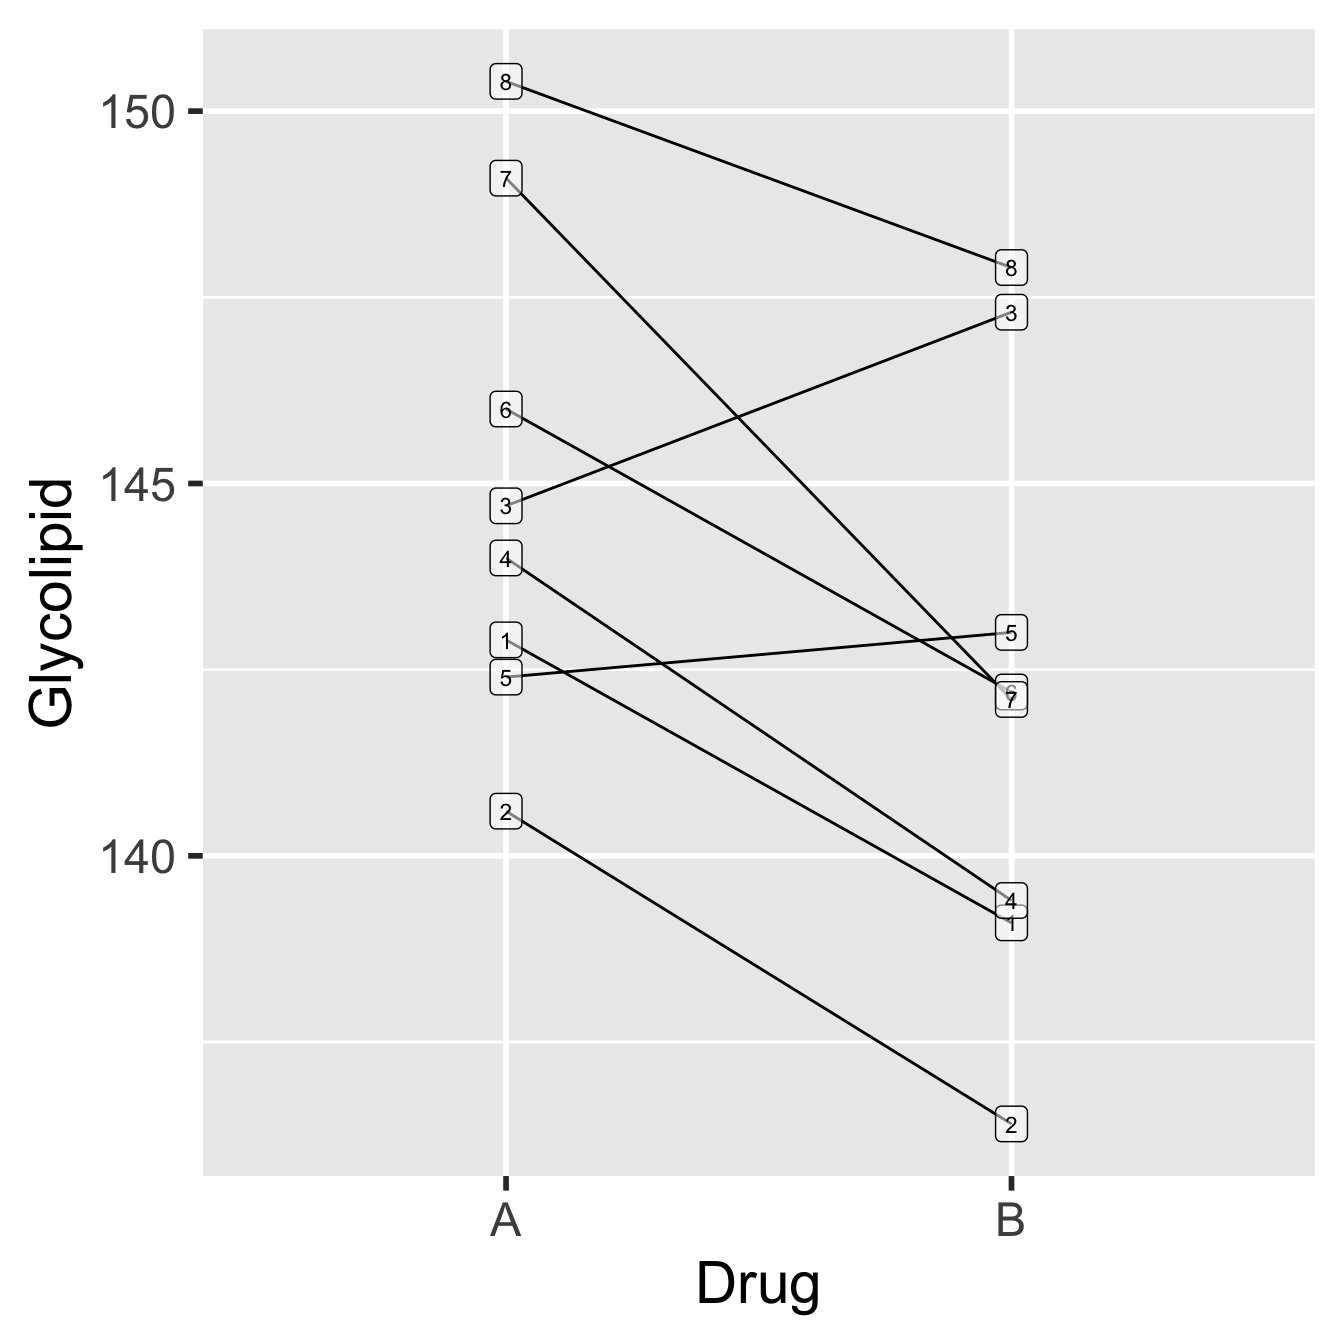
\includegraphics[width=0.5\linewidth]{intro-bio-stats-book_files/figure-latex/drug-linked-1} 

}

\caption{Data from glycolipid study, showing paired design. Each patient is denoted by a unique number.}\label{fig:drug-linked}
\end{figure}

Each patient is represented by a unique number (1-8). The order of the drugs in the plot does not matter---it doesn't mean that Drug A was tested before Drug B just because Drug A appears first. Notice that there is a lot of variability in these data, both in the glycolipid levels of each patient and in the amount by which the drugs differ in their effects (e.g.~the drugs have roughly equal effects for patient 5, while drug B appears to be more effective for patient 2). What can also be inferred from this pattern is that although the glycolipid levels vary a good deal between patients, Drug B seems to reduce glycolipid levels more than Drug A.

The advantage to using a paired-sample design in this case is clear if we look at the results we might have obtained on the same patients, but where they have been divided into two groups of four, giving one group Drug A and one group Drug B:

\begin{figure}

{\centering 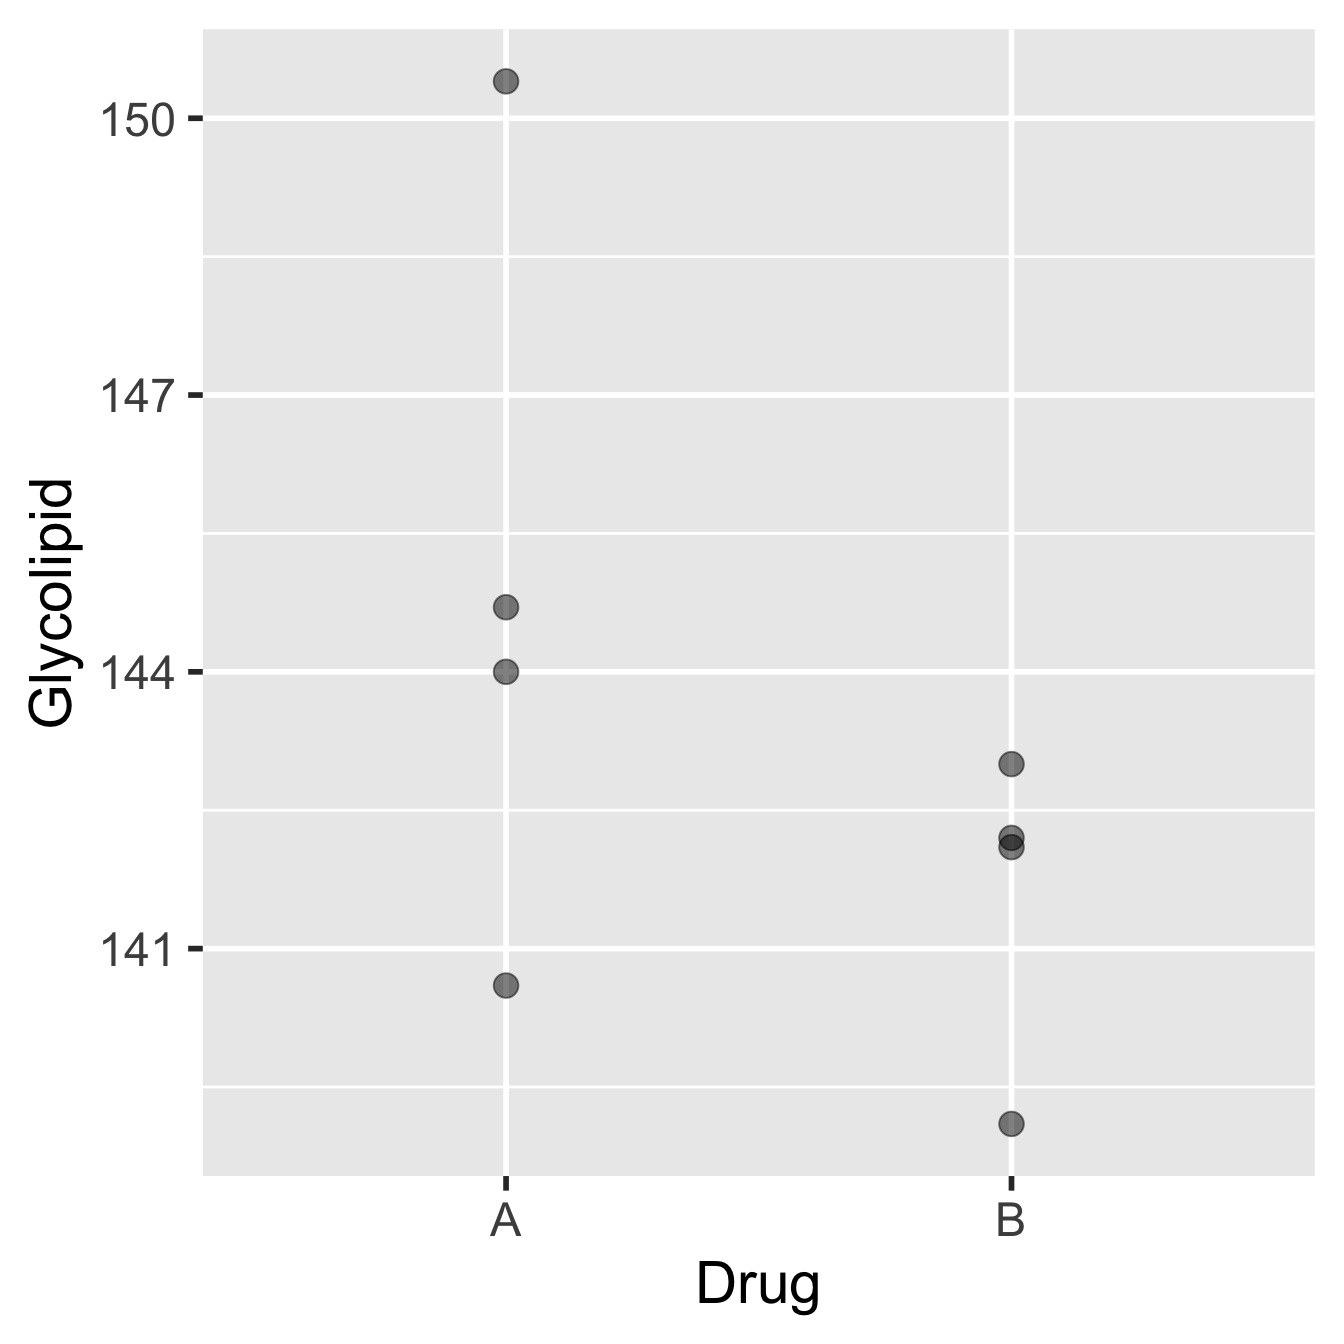
\includegraphics[width=0.5\linewidth]{intro-bio-stats-book_files/figure-latex/drug-not-linked-1} 

}

\caption{Data from glycolipid study, ignoring paired design.}\label{fig:drug-not-linked}
\end{figure}

The patients and their glycolipid levels are identical to those in the previous diagram, but now, patients 2, 3, 4 and 8 (selected at random) were given Drug A, while only patients 1, 5, 6, and 7 were given Drug B. The means of the two groups are different, with Drug B performing better, but the associated standard error are also large relative to this difference. A two-sample~\emph{t}-test would undoubtedly fail to identify a significant difference between the two drugs.

So, it would be quite possible to end up with two groups where there was no apparent difference in the mean glycolipid levels between the two drug treatments even though Drug B seems to be more effective in the majority of patients. The pairing allows us to factor out (i.e.~remove) the variation among individuals and concentrate on the differences between the two treatments. This works by focussing on the differences occurring~\emph{within}~individuals. The result is a much more sensitive evaluation of the effect we're interested in.

The next question is, how do we go about analysing paired data in a way that properly accounts for the structure in the data?

\hypertarget{how-do-you-carry-out-a-t-test-on-paired-samples}{%
\section{\texorpdfstring{How do you carry out a \emph{t}-test on paired samples?}{How do you carry out a t-test on paired samples?}}\label{how-do-you-carry-out-a-t-test-on-paired-samples}}

It should be clear why a paired-sample design might be useful, but how do we construct the right test? The `trick' is to work directly with the differences between pairs of values. In the case of the glycolipid levels illustrated in the first diagram, we noted that there was a greater decrease of glycolipids in 75\% of patients using Drug B compared with Drug A.

If we calculate the actual differences (i.e.~subtracted the value for Drug A from the value for Drug B) for each patient, we might see something like: -3.9, -4.1, 2.5, -4.7, 0.5, -3.7, -6.9, -2.4. Notice that there are only two positive values in this sample of differences, one of which is close to 0. The mean difference is -2.8, i.e.~on average, glycolipid levels are lower with Drug B. Another way of stating this observation is that \emph{within subjects} (patients), the mean difference between drug B and drug A is negative. A paired-sample design focusses on the within-subject (or more generally, within-item) change.

On the other hand, if the two drugs had had similar effects, what would we expect to see? We would expect no consistent difference in glycolipid levels between the Drug A and Drug B treatments. Glycolipid levels are unlikely to remain exactly the same over time. Still, there shouldn't be any pattern to these changes with respect to the drug treatment: some patients will show increases, some decreases, and some no change at all. The mean of the differences, in this case, should be somewhere around zero (though sampling variation will ensure it isn't exactly equal to zero).

So, to carry out a \emph{t}-test on paired-sample data, we have to: 1) find the mean of the difference of all the pairs and 2) evaluate whether this is significantly different from zero. We already know how to do this! \textbf{This is just an application of the one-sample \emph{t}-test}, where the expected value (i.e.~the null hypothesis) is 0. The thing to realise is that although we started out with two sets of values, what matters is the sample of differences between pairs and the population we're interested in a `population of differences'.

When used to analyse paired data in this way, the test is referred to as a paired-sample~\emph{t}-test. This is not wrong, but it is important to remember that a paired-sample~\emph{t}-test is just a one-sample~\emph{t}-test applied to the sample of differences between pairs of associated observations. A paired-sample~\emph{t}-test isn't a new kind of test. Instead, it is a one-sample~\emph{t}-test applied to~\emph{a particular kind of situation}.

\hypertarget{assumptions-of-the-paired-sample-t-test}{%
\subsection{\texorpdfstring{Assumptions of the paired-sample \emph{t}-test}{Assumptions of the paired-sample t-test}}\label{assumptions-of-the-paired-sample-t-test}}

The assumptions of a paired-sample~\emph{t}-test are no different from the one-sample~\emph{t}-test. After all, they boil down to the same test! We just have to be aware of the target sample. The key point to keep in mind is that the sample of differences is important, not the original data. There is no requirement for the original data to be drawn from a normal distribution because the normality assumption applies to the differences. This is very useful because even where the original data seem to be drawn from a non-normal distribution, the differences between pairs can often be acceptably normal. The differences need to be measured on an interval or ratio scale, but this is guaranteed if the original data are on one of these scales.

\hypertarget{carrying-out-a-paired-sample-t-test-in-r}{%
\section{\texorpdfstring{Carrying out a paired-sample \emph{t}-test in R}{Carrying out a paired-sample t-test in R}}\label{carrying-out-a-paired-sample-t-test-in-r}}

R offers the option of a paired-sample \emph{t}-test to save us the effort of calculating differences. It does this for us and then carries out a one-sample test on those differences. We'll look at how to do it the `old fashioned' way first---calculating the differences ourselves and running a one-sample test---before using the short-cut method provided by R. We'll do this using the glycolipid drug example.

\begin{infobox}{action}

\hypertarget{section-10}{%
\subsubsection*{}\label{section-10}}
\addcontentsline{toc}{subsubsection}{}

The data live in the `GLYCOLIPID.CSV' file. The code below assumes those data have been read into a tibble called \texttt{glycolipid}. Set that up if you plan to work along.

\end{infobox}

We start by looking at the data:

\begin{Shaded}
\begin{Highlighting}[]
\FunctionTok{glimpse}\NormalTok{(glycolipid)}
\end{Highlighting}
\end{Shaded}

\begin{verbatim}
## Rows: 16
## Columns: 4
## $ Patient    <dbl> 1, 2, 3, 4, 5, 6, 7, 8, 1, 2, 3, 4, 5, 6, 7, 8
## $ Sex        <chr> "Male", "Female", "Male", "Female", "Female", "Male", "Fema~
## $ Drug       <chr> "A", "A", "A", "A", "A", "A", "A", "A", "B", "B", "B", "B",~
## $ Glycolipid <dbl> 142.9, 140.6, 144.7, 144.0, 142.4, 146.0, 149.1, 150.4, 139~
\end{verbatim}

There are four variables in this data set: \texttt{Patient} indexes the patient identity, \texttt{Sex} is the sex of the patient (we don't need this), \texttt{Drug} denotes the drug treatment, and \texttt{Glycolipid} is the glycolipid level.

Next, we need to calculate the differences between each pair. We can do this with the \texttt{dplyr} functions \texttt{group\_by} and \texttt{summarise}:

\begin{Shaded}
\begin{Highlighting}[]
\NormalTok{glycolipid\_diffs }\OtherTok{\textless{}{-}} 
\NormalTok{  glycolipid }\SpecialCharTok{\%\textgreater{}\%}
  \FunctionTok{group\_by}\NormalTok{(Patient) }\SpecialCharTok{\%\textgreater{}\%}
  \FunctionTok{summarise}\NormalTok{(}\AttributeTok{Difference =} \FunctionTok{diff}\NormalTok{(Glycolipid))}
\end{Highlighting}
\end{Shaded}

What we did was group the data by the values of \texttt{Patient}, and then used a function called \texttt{diff} to calculate the difference between the two Glycolipid concentrations \emph{within each patient}. We stored the result of this calculation in a new data frame called \texttt{glycolipid\_diffs}. This is the data we'll use to carry out the paired-sample \emph{t}-test:

\begin{Shaded}
\begin{Highlighting}[]
\NormalTok{glycolipid\_diffs}
\end{Highlighting}
\end{Shaded}

\begin{verbatim}
## # A tibble: 8 x 2
##   Patient Difference
##     <dbl>      <dbl>
## 1       1     -3.80 
## 2       2     -4.20 
## 3       3      2.60 
## 4       4     -4.60 
## 5       5      0.600
## 6       6     -3.80 
## 7       7     -7    
## 8       8     -2.5
\end{verbatim}

We should check that the differences could plausibly have been drawn from a normal distribution, though keep in mind that the normality assumption is hard to assess with only 8 observations:

\begin{Shaded}
\begin{Highlighting}[]
\FunctionTok{ggplot}\NormalTok{(glycolipid\_diffs, }\FunctionTok{aes}\NormalTok{(}\AttributeTok{x =}\NormalTok{ Difference)) }\SpecialCharTok{+}
  \FunctionTok{geom\_dotplot}\NormalTok{() }\SpecialCharTok{+} \FunctionTok{theme\_grey}\NormalTok{(}\AttributeTok{base\_size =} \DecValTok{22}\NormalTok{)}
\end{Highlighting}
\end{Shaded}

\begin{verbatim}
## Bin width defaults to 1/30 of the range of the data. Pick better value with `binwidth`.
\end{verbatim}

\begin{figure}

{\centering 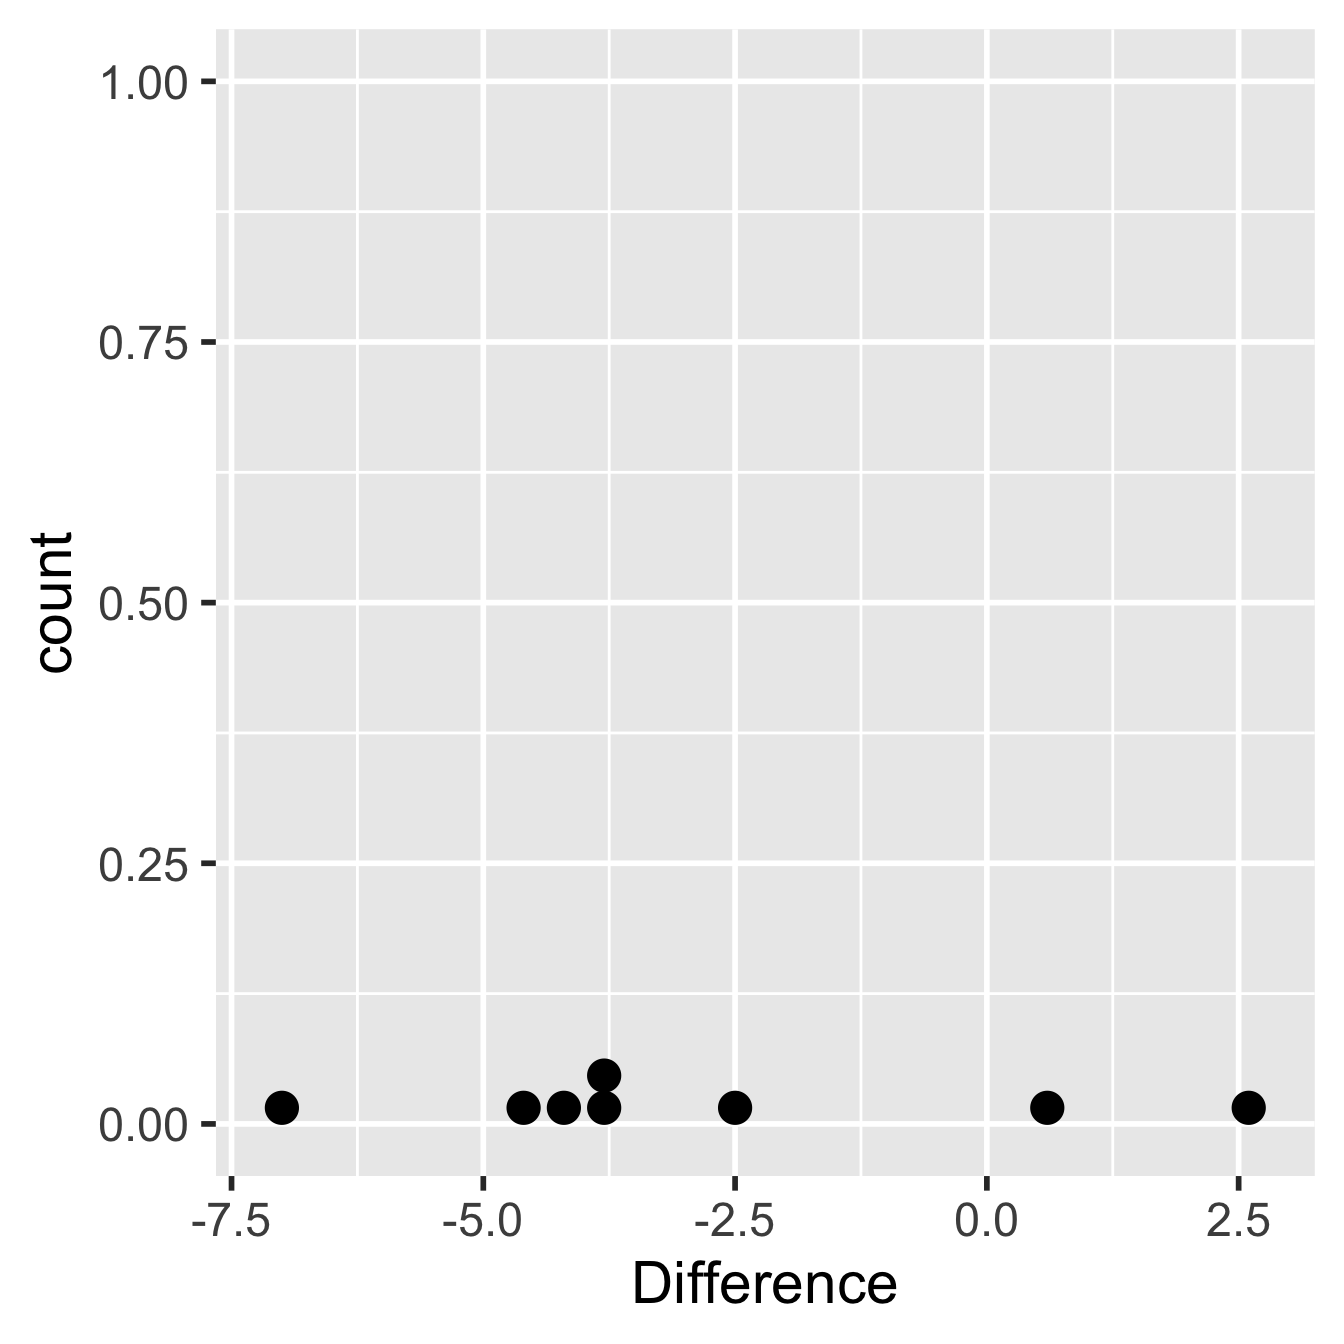
\includegraphics[width=0.5\linewidth]{intro-bio-stats-book_files/figure-latex/glyco-diffs-1} 

}

\caption{Within-individual differences from glycolipid study}\label{fig:glyco-diffs}
\end{figure}

Hmm\ldots{} there really isn't a lot of data to work with here but there's nothing in that plot that screams `non-normal', which means the assumptions have been met as best they can be. Let's proceed to carry out a one-sample \emph{t}-test on the calculated differences. This is easy to do in R:

\begin{Shaded}
\begin{Highlighting}[]
\FunctionTok{t.test}\NormalTok{(glycolipid\_diffs}\SpecialCharTok{$}\NormalTok{Difference)}
\end{Highlighting}
\end{Shaded}

\begin{verbatim}
## 
##  One Sample t-test
## 
## data:  glycolipid_diffs$Difference
## t = -2.6209, df = 7, p-value = 0.03436
## alternative hypothesis: true mean is not equal to 0
## 95 percent confidence interval:
##  -5.397549 -0.277451
## sample estimates:
## mean of x 
##   -2.8375
\end{verbatim}

We don't have to set the \texttt{data} argument to carry out a one-sample \emph{t}-test on the differences. We just passed along the numeric vector of differences extracted from \texttt{glycolipid\_diffs} (using the \texttt{\$} operator). What happened to the \texttt{mu} argument used to set up the null hypothesis? Remember, the null hypothesis is that the population mean is zero. R assumes that this is 0 if we don't supply it, so no need to set it here.

The output is quite familiar\ldots{} The first line reminds us what kind of test we did, and the second line reminds us what data we used to carry out the test. The third line is the important one: \texttt{t\ =\ -2.6209,\ df\ =\ 7,\ *p*-value\ =\ 0.03436}. This gives the \emph{t}-statistic, the degrees of freedom, and the all-important \emph{p}-value associated with the test. The \emph{p}-value tells us that the mean within-individual difference is significant at the \emph{p} \textless{} 0.05 level.

We need to express these results in a clear sentence incorporating the relevant statistical information:

\begin{quote}
Individual patients had significantly lower serum glycolipid concentrations when treated with Drug B than when treated with Drug A (\emph{t} = 2.62, d.f. = 7, \emph{p} \textless{} 0.05).
\end{quote}

There are a couple of things to point out in interpreting the result of such a test:

\begin{enumerate}
\def\labelenumi{\arabic{enumi}.}
\item
  The sample of differences was used in the test, not the sample of paired observations. This means the degrees of freedom for a paired-sample \emph{t} test are one less than the number of differences (= number of pairs); not one, or two, less than the total number of observations.
\item
  Since we used a paired-sample design our conclusion stresses the fact that the use of the Drug B results in a lower glycolipid level in individual patients. It doesn't say that the use of Drug B resulted in lower glycolipid concentrations for everyone given Drug B than for anyone given Drug A.
\end{enumerate}

\hypertarget{using-the-paired-true-argument}{%
\subsection{\texorpdfstring{Using the \texttt{paired\ =\ TRUE} argument}{Using the paired = TRUE argument}}\label{using-the-paired-true-argument}}

R has a built-in procedure for doing paired-sample~\emph{t}-tests in one step. Now that we've done it the hard way, let's try carrying out the test using that built-in procedure. This looks very similar to a two-sample \emph{t}-test, except that we have to set the \texttt{paired} argument of the \texttt{t.test} function to \texttt{TRUE}:

\begin{Shaded}
\begin{Highlighting}[]
\FunctionTok{t.test}\NormalTok{(Glycolipid }\SpecialCharTok{\textasciitilde{}}\NormalTok{ Drug, }\AttributeTok{data =}\NormalTok{ glycolipid, }\AttributeTok{paired =} \ConstantTok{TRUE}\NormalTok{)}
\end{Highlighting}
\end{Shaded}

\begin{verbatim}
## 
##  Paired t-test
## 
## data:  Glycolipid by Drug
## t = 2.6209, df = 7, p-value = 0.03436
## alternative hypothesis: true difference in means is not equal to 0
## 95 percent confidence interval:
##  0.277451 5.397549
## sample estimates:
## mean of the differences 
##                  2.8375
\end{verbatim}

R takes care of the differencing for us, so now we can work with the original \texttt{glycolipid} data rather than the \texttt{glycolipid\_diffs} data frame constructed above. We won't step through the output because it should make sense by this point.

\begin{infobox}{action}

\hypertarget{order-matter}{%
\subsubsection*{Order matter!}\label{order-matter}}
\addcontentsline{toc}{subsubsection}{Order matter!}

Be careful when using the built in procedure for doing paired-sample \emph{t}-tests. The only information R uses to associate pairs of observations is their order in each group. The first observation in the `A' group is paired with the first observation in the `B' group, the second observation in the `A' group is paired with the second observation in the `B' group, and so on. If the items/individuals aren't ordered the same way in each group, the test will be wrong and we'll end up with a meaningless \emph{p}-value!

\end{infobox}

It's nice that R makes it easy to do a paired-sample \emph{t}-test in one step. Just don't forget that this version of the \emph{t}-test is just a one-sample test on paired differences.

\hypertarget{anova-for-randomised-block-designs}{%
\chapter{ANOVA for randomised block designs}\label{anova-for-randomised-block-designs}}

\begin{quote}
\emph{Block what you can; randomize what you cannot.}

George Box
\end{quote}

\hypertarget{randomised-complete-block-designs}{%
\section{Randomised Complete Block Designs}\label{randomised-complete-block-designs}}

We have only considered one type of experimental ANOVA design up until now: the \textbf{Completely Randomised Design} (CRD). The defining feature of a CRD is that treatments are assigned completely at random to experimental units. This is the simplest type of experimental design. Randomisation is a good thing because it prevents systematic biases from creeping in. A CRD approach is often `good enough' in many situations. However, it isn't necessarily the most powerful design---if at all possible, we should use \textbf{blocking} to account for \textbf{nuisance factors}. A nuisance factor affects the response---it creates variation---but is of no interest to the experimenter. The variability induced by nuisance factors should be accounted for at the design stage of an experiment if possible. Let's consider a hypothetical experiment to remind ourselves how blocking works.

Imagine we're evaluating the effect of three different fertiliser application rates on wheat yields (t/ha). We suspect that our experimental fields' soil type and management histories are quite different, leading to significant `field effects' on yield. We don't care about these field effects---they are a nuisance---but we'd like to account for them. There are two factors in play in this setting: the first is the set of experimental treatments (fertiliser application rate); the second is the source of nuisance variation (field). Fertiliser application rate is the `treatment factor', and field is the `blocking factor'.

Here is one way to block the experiment. The essence of the design is that a set of fields are chosen, which may differ in various unknown conditions (soil water, aspect, disturbance, etc.), and within each field, three plots are set up. Each plot receives one of the three fertiliser rate treatments at random. If we chose to work with eight fields, the resulting data might look like this:

\begin{longtable}[]{@{}rllll@{}}
\toprule
& \textbf{Fertilizer} & Control & Absent & High \\
\midrule
\endhead
\textbf{Block} & Field 1 & 9.3 & 8.7 & 10.0 \\
& Field 2 & 8.7 & 7.1 & 9.1 \\
& Field 3 & 9.3 & 8.2 & 10.4 \\
& Field 4 & 9.5 & 8.9 & 10.0 \\
& Field 5 & 9.9 & 9.1 & 10.8 \\
& Field 6 & 8.9 & 8.0 & 9.0 \\
& Field 7 & 8.3 & 6.2 & 8.9 \\
& Field 8 & 9.1 & 7.0 & 8.1 \\
\bottomrule
\end{longtable}

Each treatment level is represented in each field (block), but only once. The experiment is `blocked by field'. Now consider these two questions:

\begin{itemize}
\item
  Why is this design useful? Blocking allows us to partition out the environmental variation due to different field conditions. For example, the three treatments in field 5 produced a relatively high yield, while the yields in field 7 are consistently below average within each treatment. This among field variation is real, and if we hadn't blocked the experiment, it would appear as a `noise' component of our analysis. But since we blocked the experiment, and every treatment is present in every block, we can `remove' the block variation from the noise. Less noise means more statistical power.
\item
  Why is each treatment level represented only once within blocks? This design gives us the best chance of generalising our results. If we are interested in the overall effect of fertiliser, we should prefer to put our effort into including a range of possible environmental conditions. If we only did the experiment in one field, the results might turn out to be rather unusual. We are not interested in the environmental variation as such. We want to know for a range of conditions, whatever they might be, whether there are consistent differences between fertiliser application rates.
\end{itemize}

There are many different ways to introduce blocking into an experiment. The most commonly used design---and the one that is easiest to analyse---is called a \textbf{Randomised Complete Block Design}. The defining feature of this design is that \emph{each block sees each treatment exactly once}. The fertiliser study is an example of a Randomised Complete Block Design (RCBD). The obvious question is: How do we analyse an RCBD? We'll explore that in moment. First, a small detour\ldots.

\hypertarget{analysing-an-rcbd-experiment}{%
\section{Analysing an RCBD experiment}\label{analysing-an-rcbd-experiment}}

Let's consider a new example to drive home how an RCBD works. We want to assess whether there is a difference in the impact that the predatory larvae of three damselfly species (\emph{Enallagma}, \emph{Lestes} and \emph{Pyrrhosoma}) have on the abundance of midge larvae in a pond. We plan to conduct an experiment in which small (1 m\textsuperscript{2}) nylon mesh cages are set up in the pond. All damselfly larvae will be removed from the cages and each cage will then be stocked with 20 individuals of one of the species. After 3 weeks, we will sample the cages and count the density of midge larvae in each. We have 12 cages altogether, so four replicates of each of the three species can be established.

On the face of it, this looks like a one-way design with each species as a treatment. The only problem to resolve is how to distribute the enclosures in the pond. The pond is unlikely to be uniform in depth, substrate, temperature, shade, etc\ldots{} Some of the variation will be obvious, some will not. We have two options: 1) use a CRD and distribute the cages at random, or 2) adopt an RCBD by grouping the cages into clusters of three, placing each cluster at a randomly chosen location, and assigning the three treatments to cages at random within each cluster. These are illustrated below (left = CRD, right = RCBD):

\begin{center}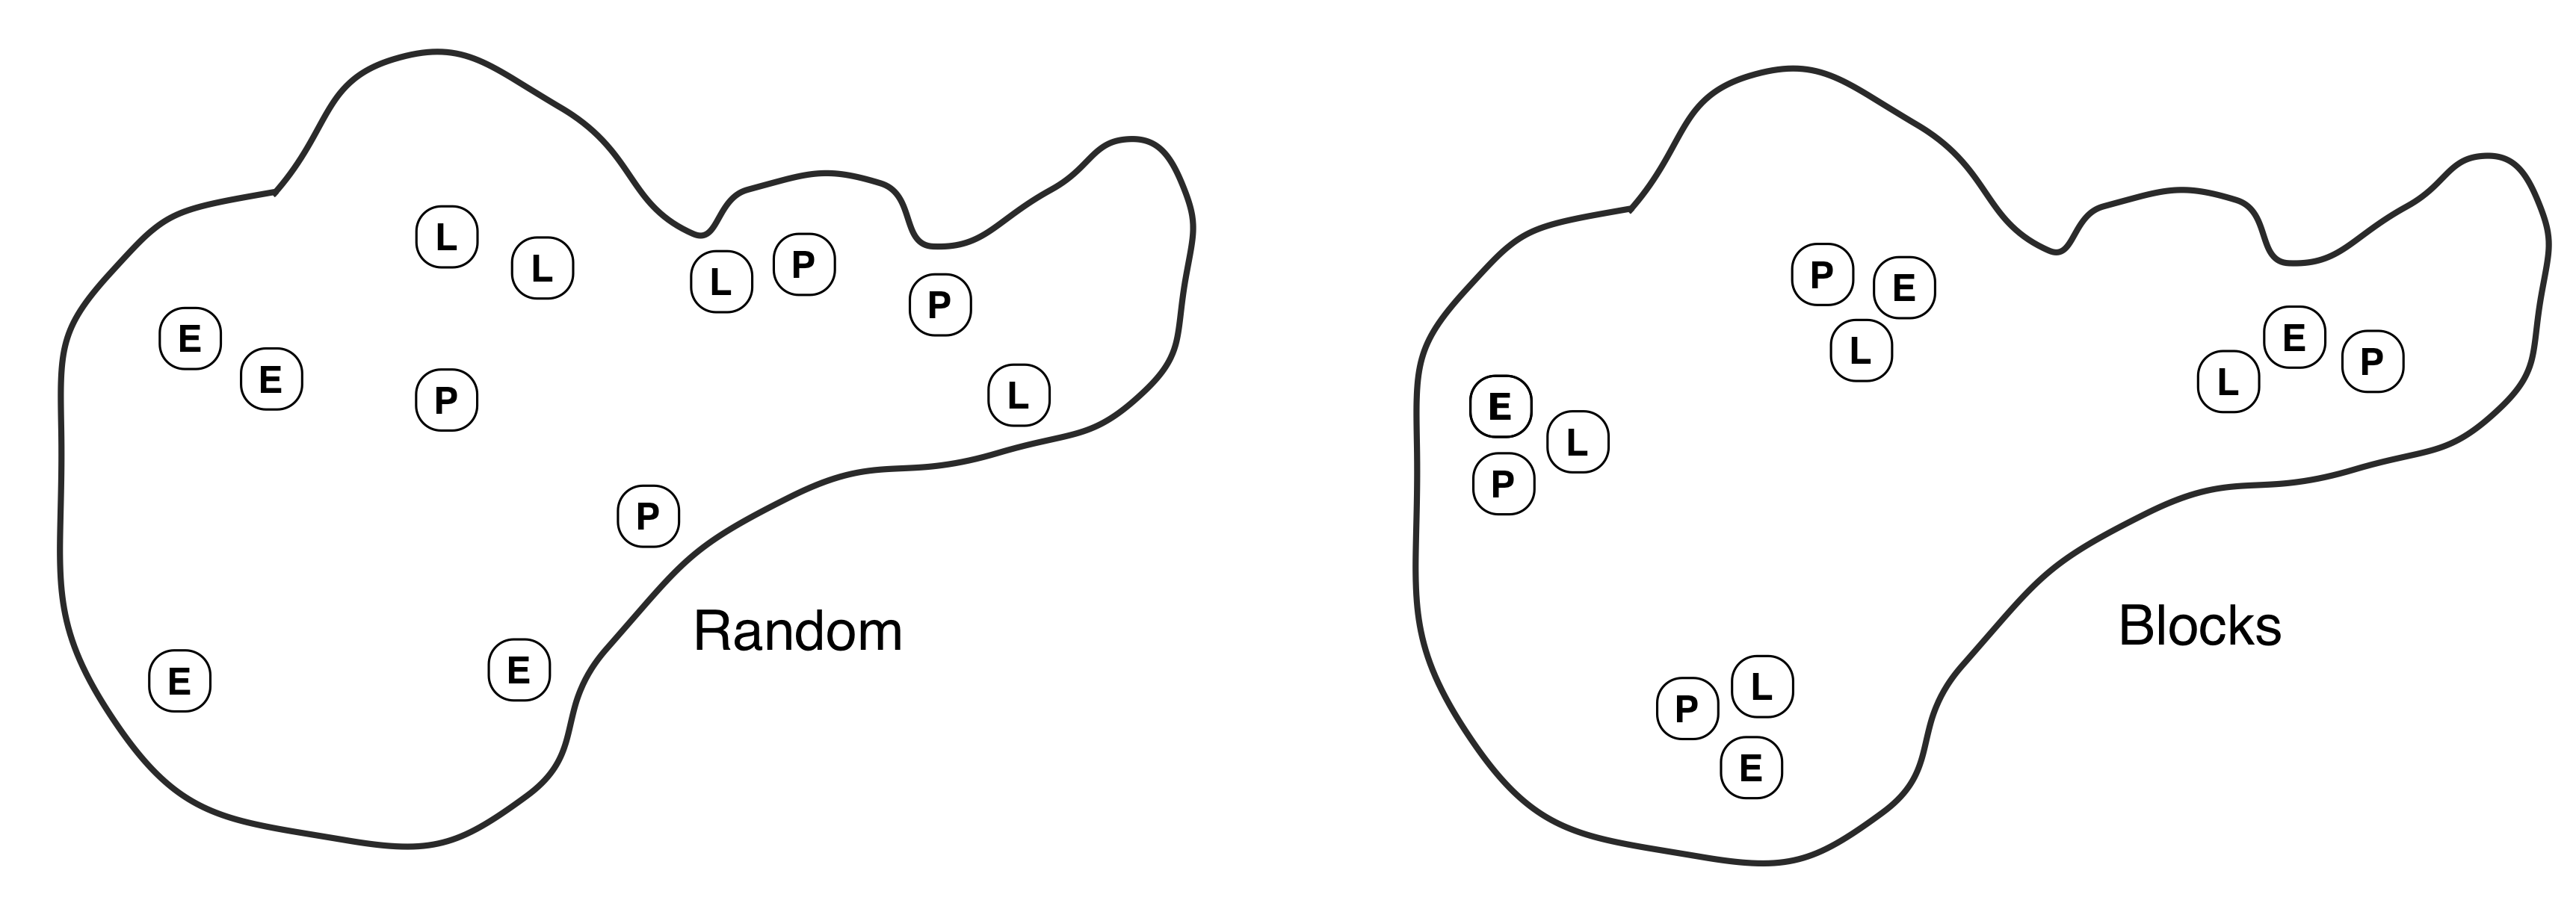
\includegraphics[width=0.75\linewidth]{./images/damselfly-expt-layouts} \end{center}

What are the consequences of the two alternatives? If the cages are distributed at random (CRD), they will cover a wide range of variation in these factors. These sources of variation will almost certainly cause the density of midge larvae to vary around the pond unpredictably, increasing the noise in the data. If we group sets of treatments into clusters, we are creating `spatial blocks'. There may be considerable differences between blocks, but these won't obscure differences between the treatments because all three treatments are present in every block.

\hypertarget{carrying-out-the-analysis-with-r}{%
\section{Carrying out the analysis with R}\label{carrying-out-the-analysis-with-r}}

We'll now illustrate how to analyse data from an RCBD experiment using the damselfly predation example.

\begin{infobox}{action}

\hypertarget{section-11}{%
\subsubsection*{}\label{section-11}}
\addcontentsline{toc}{subsubsection}{}

The data live in the `DAMSELS.CSV' file. The code below assumes those data have been read into a tibble called \texttt{damsels}. Set that up if you plan to work along.

\end{infobox}

The density of midge larvae in each enclosure after 3 weeks are in the \texttt{Midge} variable (number m\(^{-2}\)); codes for species in the \texttt{Species} variable (levels: \emph{Enallagma}, \emph{Lestes} and \emph{Pyrrhosoma}), and the block identities (A, B, C, D) in the third column:

\begin{Shaded}
\begin{Highlighting}[]
\FunctionTok{glimpse}\NormalTok{(damsels)}
\end{Highlighting}
\end{Shaded}

\begin{verbatim}
## Rows: 12
## Columns: 3
## $ Midge   <dbl> 304, 464, 320, 578, 509, 458, 680, 740, 630, 356, 390, 350
## $ Species <chr> "Enallagma", "Lestes", "Pyrrhosoma", "Enallagma", "Lestes", "P~
## $ Block   <chr> "A", "A", "A", "B", "B", "B", "C", "C", "C", "D", "D", "D"
\end{verbatim}

The process of analysing an RCBD experiment is essentially the same as any other type of ANOVA. First, we fit the model using the \texttt{lm} function, and then we use \texttt{anova} to calculate \emph{F}-statistics, degrees of freedom, and \emph{p}-values:

\begin{Shaded}
\begin{Highlighting}[]
\NormalTok{damsels.model }\OtherTok{\textless{}{-}} \FunctionTok{lm}\NormalTok{(Midge }\SpecialCharTok{\textasciitilde{}}\NormalTok{ Species }\SpecialCharTok{+}\NormalTok{ Block, }\AttributeTok{data =}\NormalTok{ damsels)}
\FunctionTok{anova}\NormalTok{(damsels.model)}
\end{Highlighting}
\end{Shaded}

We suppressed the output for now. Notice that we have put two factors on the right-hand side of the \texttt{\textasciitilde{}} symbol. This tells R that we want to fit a model that accounts for the main effects of \texttt{Species} and \texttt{Block}. We have to put a \texttt{+} between terms to delineate them (this is not optional).

\begin{infobox}{warning}

\hypertarget{careful-with-your-and}{%
\subsubsection*{\texorpdfstring{Careful with your \texttt{+} and \texttt{*}}{Careful with your + and *}}\label{careful-with-your-and}}
\addcontentsline{toc}{subsubsection}{Careful with your \texttt{+} and \texttt{*}}

Notice that we used the `plus' symbol (\texttt{+}) to include the blocking factor in the model: \texttt{Species\ +\ Block}. R also allows us to use the `times' symbol (\texttt{*}) in a model formula, e.g.~\texttt{Species\ *\ Block}. However, this formulation is not appropriate for including block effects. It is used to set up models for more complicated designs that involve something called an interaction term. We're not going to cover those in this book, so for now, make a mental note of the fact that blocking factors must be included via the \texttt{+} symbol.

And by the way\ldots{} the \texttt{+} has nothing to do with addition when working a model specification in R.

\end{infobox}

Here are the results of the global significance tests using the correct ANOVA model for our randomised block experiment:

\begin{Shaded}
\begin{Highlighting}[]
\FunctionTok{anova}\NormalTok{(damsels.model)}
\end{Highlighting}
\end{Shaded}

\begin{verbatim}
## Analysis of Variance Table
## 
## Response: Midge
##           Df Sum Sq Mean Sq F value    Pr(>F)    
## Species    2  14904    7452  3.0053 0.1246687    
## Block      3 208425   69475 28.0182 0.0006306 ***
## Residuals  6  14878    2480                      
## ---
## Signif. codes:  0 '***' 0.001 '**' 0.01 '*' 0.05 '.' 0.1 ' ' 1
\end{verbatim}

What does all this mean? We interpret each line of the ANOVA table in exactly the same way as we do for a one-way ANOVA. The first part tells us what kind of output we are looking at:

\begin{verbatim}
## Analysis of Variance Table 
##  
## Response: Midge
\end{verbatim}

This reminds us that we are looking at an ANOVA table where our response variable was called \texttt{Midge}. The table contains the key information:

\begin{verbatim}
##           Df Sum Sq Mean Sq F value    Pr(>F)     
## Species    2  14904    7452  3.0053 0.1246687     
## Block      3 208425   69475 28.0182 0.0006306 *** 
## Residuals  6  14878    2480
\end{verbatim}

This ANOVA table is similar to the ones we have already seen, except that we now have to consider two lines---one for each term in the model. The first is for the main effect of Species and the second for the main effect of Block.

The \emph{F}-ratio is the test statistic for each term. These provide a measure of how large and consistent the effects associated with each term are. Each \emph{F}-ratio has a pair of degrees of freedom associated with it: one belonging to the term itself, the other due to the error (residual). Together, the \emph{F}-ratio and its degrees of freedom determine the \emph{p}-value.

The \emph{p}-value gives the probability that the differences between the set of means for each term in the model, or a more extreme difference, could have arisen through sampling variation under the null hypothesis of no difference. We take \emph{p} \textless{} 0.05 as evidence that at least one of the treatments is having an effect. Here, there is a significant effect of block (\emph{p} \textless{} 0.001), which says that the density of midge larvae varies across the lake. It looks like blocking was a good idea---there is a lot of spatial (nuisance) variation in midge larvae density. However, what we care about is the damselfly species effect. This term is not significant (\emph{p} \textgreater{} 0.05), so we conclude that there is no difference in the impact of the predatory larvae of three damselfly species.

It is instructive to see what happens if we analyse the damselfly data as though they are from a one-way design. We do this by including only the experimental treatment term (Species) in the model:

\begin{Shaded}
\begin{Highlighting}[]
\NormalTok{damsels.oneway }\OtherTok{\textless{}{-}} \FunctionTok{lm}\NormalTok{(Midge }\SpecialCharTok{\textasciitilde{}}\NormalTok{ Species, }\AttributeTok{data =}\NormalTok{ damsels)}
\FunctionTok{anova}\NormalTok{(damsels.oneway)}
\end{Highlighting}
\end{Shaded}

\begin{verbatim}
## Analysis of Variance Table
## 
## Response: Midge
##           Df Sum Sq Mean Sq F value Pr(>F)
## Species    2  14904  7452.1  0.3003 0.7477
## Residuals  9 223303 24811.4
\end{verbatim}

Look at the degrees of freedom and the sums of squares of the residual (error). How do these compare to the previous model that accounted for the block effect? The degrees of freedom is higher. In principle, this is a good thing because it means we have more power to detect a significant difference among the treatment means. However, the error sum of squares is also much higher when we ignore the block effect. We accounted for much less noise by ignoring the block effect. As a result, the error mean square is a lot lower, and so the \emph{F}-statistic associated with the treatment effect is also much lower. The take-home message is that designing a blocked experiment and properly accounting for the blocked structure will result in a more powerful analysis.

\hypertarget{are-there-disadvantages-to-randomised-block-designs}{%
\section{Are there disadvantages to randomised block designs?}\label{are-there-disadvantages-to-randomised-block-designs}}

The short answer is no, not really. There are instances when a randomised block design might appear to be disadvantageous at first glance, but these don't stand up to criticism:

\begin{enumerate}
\def\labelenumi{\arabic{enumi}.}
\item
  What if we want to know if the effect of treatment varies across blocks? For example, we might be interested in whether or not damselfly effects on the midge densities are consistent in all habitat areas (e.g.~some species may forage more effectively in muddy areas, others where there are more leaves). If this is the question we are trying to answer, we should have designed a different experiment. For example, a design in which we consider treatment combinations of different midge species and habitat characteristics might be appropriate. Fundamentally, the goal of blocking is to account for \emph{uncontrolled} variation. Designing a blocked experiment and then lamenting the fact that we can't fully evaluate differences among blocks is a good example of trying to ``have our cake and eat it too''.
\item
  If the blocking term does not account for some variation, the analysis may be slightly less powerful than just using a one-way ANOVA. This is because there are fewer error degrees of freedom associated with the blocked analysis (we lose a few to the block effects). This argument only works if the block effect accounts for minimal variation. We can never know before we start an experiment whether or not blocking is needed, but we do know that biological systems are inherently noisy, with many sources of uncontrolled variation coming into play. In most experimental settings, we can be fairly sure that blocking will `work'. If we choose not to block an experiment, there is no way to account for uncontrolled variation, and we will almost certainly lose statistical power as a result.
\end{enumerate}

The advice contained in the quote at the beginning of this chapter is probably the best experimental design advice ever dished out: ``Block what you can; randomize what you cannot.''

\hypertarget{multiple-blocking-factors}{%
\section{Multiple blocking factors}\label{multiple-blocking-factors}}

It is common to find ourselves in a situation whereby we need to account for more than one blocking factor. The simplest option is to combine the nuisance factors into a single factor. However, this isn't always possible or even desirable. Consider an instance where there is a single factor of primary interest (the treatment factor) and two nuisance factors. For example, imagine that we want to test the efficacy of three drugs (A, B and C) to alleviate the symptoms of a disease. Three patients are available for a trial, and each will be available for three weeks. Testing a single drug requires a week, meaning an experimental unit is a `patient-week'. The obvious question is, how should we randomise treatments across `patient-weeks'?

We have to design an experiment like this with great care, or there is a risk that we will not be able to statistically separate the treatment effects (drug) and block effects (week \& patient). The most appropriate design for this kind of experiment has the following structure:

\begin{longtable}[]{@{}clll@{}}
\toprule
& Week & Patient & Drug \\
\midrule
\endhead
& 1 & 1 & A \\
& 1 & 2 & B \\
& 1 & 3 & C \\
& 2 & 1 & C \\
& 2 & 2 & A \\
& 2 & 3 & B \\
& 3 & 1 & B \\
& 3 & 2 & C \\
& 3 & 3 & A \\
\bottomrule
\end{longtable}

This kind of experimental design is called a Latin square design. It gets its name from the fact that if we organise the treatments into the rows and columns of a grid according to week and patient number, we arrive at something like this:

\begin{verbatim}
A B C 
C A B 
B C A
\end{verbatim}

Each letter appears once in each column and row. This is called a Latin square arrangement. Latin square designs (and their more exotic friends, e.g.~`Hyper-Graeco-Latin square designs!') have a very useful property: they allow us to unambiguously separate treatment and block effects. The reasoning behind this conclusion is quite technical so we won't try to explain it. We just want to demonstrate that it is perfectly possible to block an experiment by more than one factor, though this needs to be done with care.

\hypertarget{part-checking-and-fixing-models}{%
\part{Checking and Fixing Models}\label{part-checking-and-fixing-models}}

\hypertarget{assumptions-and-diagnostics}{%
\chapter{Assumptions and diagnostics}\label{assumptions-and-diagnostics}}

We often have a statistical analysis in mind when we collect some data. Though it can be tempting to jump straight into that analysis without first examining the data, this is seldom a good idea. We began each investigation in the last few chapters by inspecting the data set to understand what it was telling us. The initial inspection also provides an opportunity to evaluate whether or not our planned analysis assumptions are likely to be violated.

Assumptions are important. We learnt in previous chapters that regression and ANOVA are special cases of the general linear model. This is a parametric model, which makes several assumptions about the data that we need to be aware of. If our data do not meet those assumptions, at least approximately, then we cannot rely on the results given by any associated tests. This chapter aims to review what those assumptions are for simple regression and regression and one-way ANOVA models.

\hypertarget{understanding-data}{%
\section{Understanding data}\label{understanding-data}}

We've been using `well-behaved' data sets in this book so far, which tends to give the impression that visual inspections of the data are not all that necessary. Here's an example of why it matters. Imagine we are interested in quantifying the relationship between two variables, called \(x\) and \(y\). We might be tempted to carry out a linear regression analysis without first inspecting these data to get straight to `the answer': the coefficients of the linear regression model. This could be very misleading. Take a look at these four scatter plots:

\begin{center}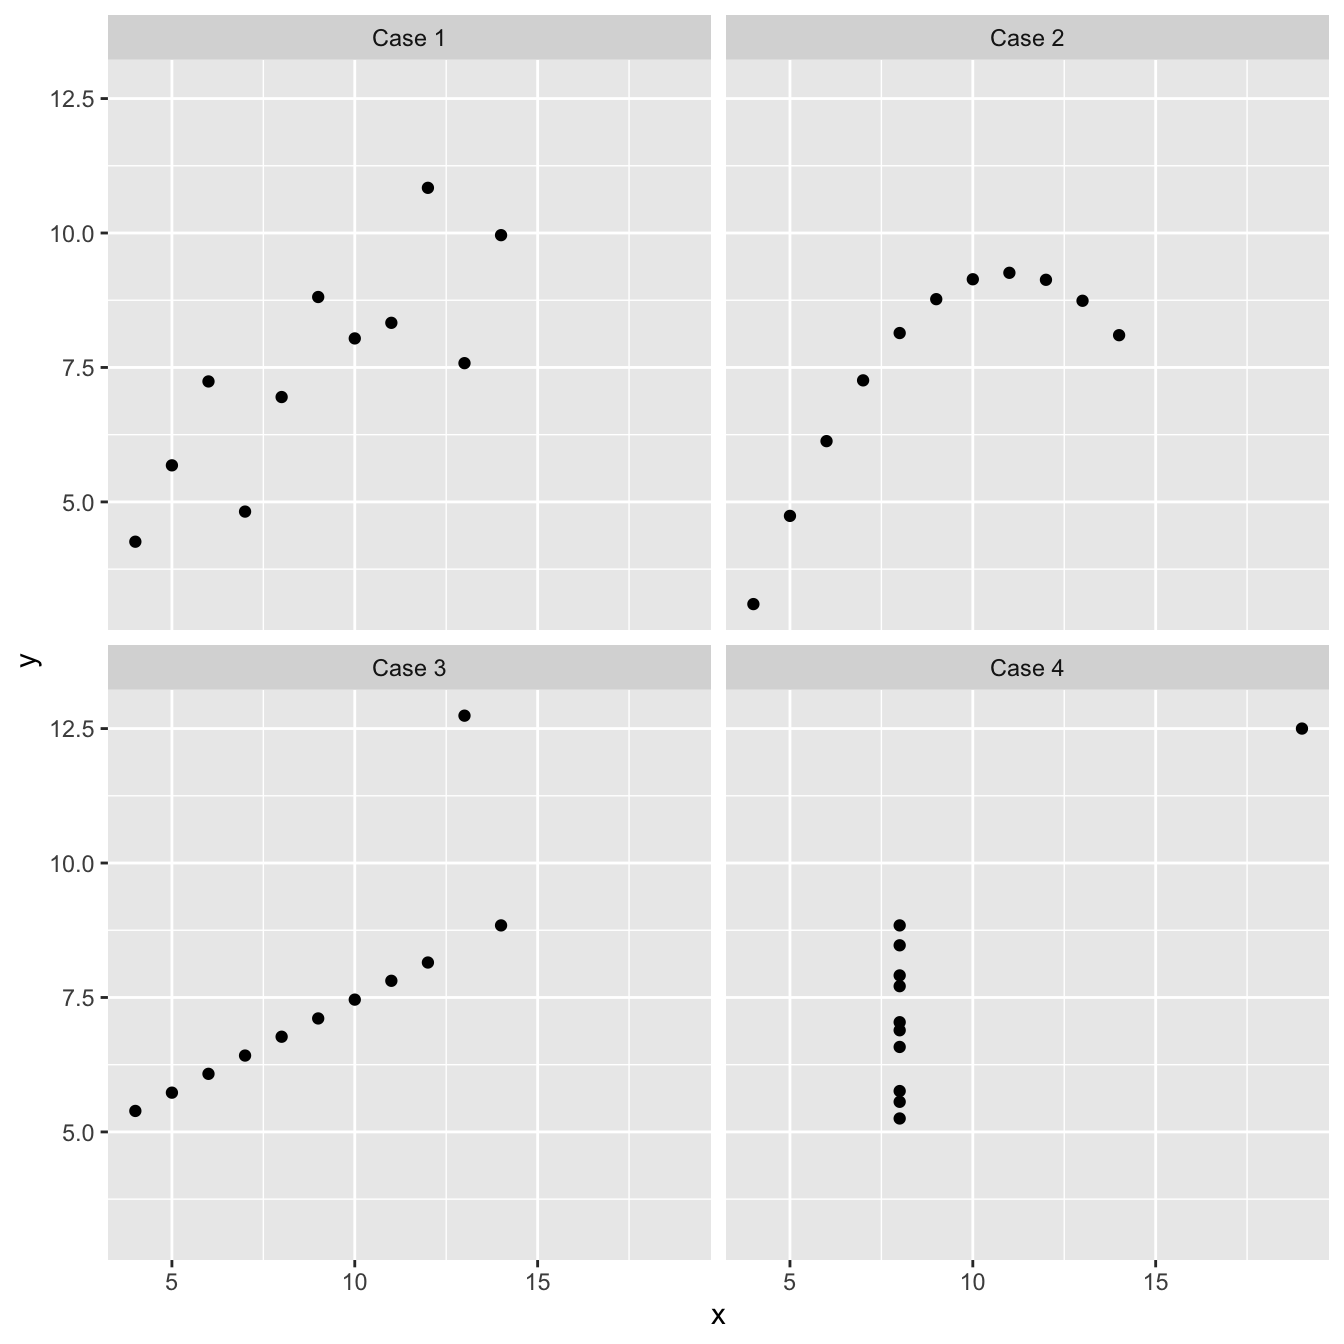
\includegraphics[width=0.6\linewidth]{intro-bio-stats-book_files/figure-latex/unnamed-chunk-152-1} \end{center}

These four artificial data sets were constructed by the statistician Francis Anscombe. The means and variances of \(x\) and \(y\) are nearly identical in all four data sets. What's more, the intercepts and slopes of the best fit regression lines are almost identical---they are 3.0 and 0.5, respectively. The nature of the relationship between \(x\) and \(y\) is quite obviously different among the four cases:

\begin{enumerate}
\def\labelenumi{\arabic{enumi}.}
\item
  ``Case 1'' shows two linearly related, normally distributed variables. This is the kind of data we often hope for in a statistical analysis.
\item
  ``Case 2'' shows two variables that are not normally distributed, but there is a perfect non-linear relationship between the two.
\item
  ``Case 3'' shows an example the variables are perfectly linearly associated for all but one observation which ruins the perfect relationship.
\item
  ``Case 4'' shows an example where a single outlier generates an apparent relationship where the two variables are otherwise unrelated.
\end{enumerate}

Each plot tells a different story about the relationship between \(x\) and \(y\), yet the linear regression model says the relationship is the same in each case. These are obviously somewhat pathological examples, but they illustrate the kinds of issues that can, and do, arise with real data. There is a real risk we will apply an inappropriate analysis if we fail to detect these kinds of problems.

Every statistical model makes certain assumptions about the data\footnote{Even so-called `non-parametric' models have underpinning assumptions; these are just not as restrictive as their parametric counterparts.}. Even if a dataset doesn't exhibit the pronounced problems seen in the Anscombe examples, we still need to assess whether the assumptions of the statistical model we want to use are likely to be valid. For example, when working with a linear regression model, we started with a scatter plot of the response variable vs the predictor variable. This allowed us to assess whether the two variables are linearly related. However, as we noted at the time, linearity is not the only assumption we need to consider when carrying out a linear regression. In the rest of this chapter, we'll go through the remaining regression assumptions and then consider the assumptions for a one-way ANOVA.

In the later regression diagnostics chapters, we'll move on to how to check whether these assumptions are valid with your data.

\hypertarget{assumptions-of-regression}{%
\section{Assumptions of regression}\label{assumptions-of-regression}}

Let's consider each of the assumptions of a regression in their approximate order of importance:

\begin{enumerate}
\def\labelenumi{\arabic{enumi}.}
\item
  \textbf{Independence.} The residuals must be independent. Another way of stating this assumption is that the value of each residual does not depend on the value of any others. This can be difficult to check. If the data are from a carefully designed experiment, everything should be OK. If the data are observational, then we need to be a lot more careful. This assumption matters because when the residuals are not independent, any \emph{p}-values we generate will be unreliable.
\item
  \textbf{Measurement scale.} The response (\(y\)) and predictor (\(x\)) variables are measured on an interval or ratio scale. It doesn't really make sense to use categorical data in a regression\footnote{It sometimes makes sense to use a regression analysis when the predictor variable is an ordinal categorical variable. It depends what you want to do with the resulting model. However, some people disagree with this approach, so it's best to avoid doing it unless you're confident you can justify it.}. This one is easy to assess.
\item
  \textbf{Linearity.} The relationship between the predictor \(x\) variable and the response \(y\) variable is linear. There is little point in fitting a straight line to data that don't form a straight-line relationship. There may also be circumstances in which it is theoretically unlikely for a relationship to be linear, e.g.~a linear relationship will not well describe the length and weight of an animal because weight is roughly a cubic function of length. If the data fail this assumption, applying a mathematical transformation of \(x\) or \(y\) can help. We will come back to this idea in the later data transformations chapter.
\item
  \textbf{Constant variance.} The variance of the residuals is constant. This assumption essentially means the variability of the residuals is not related to the value of the predictor \(x\) variable. It is violated if the magnitude of the residuals increase or decrease markedly as \(x\) gets larger. If the data fail this assumption then again, sometimes applying a mathematical transformation of \(y\) will help.
\item
  \textbf{Normality.} The residuals are drawn from a normal distribution. This essentially means that for a particular value of \(x\) we would expect a range of responses in \(y\) which follow a normal distribution. The distribution of the deviations of \(y\) from the fitted line (the residuals) is assumed to be normal, not the raw \(y\) values. This means that we can generally only test this assumption \emph{after} the line has been fitted. It is hard to evaluate this assumption by looking at the raw data.
\item
  \textbf{Measurement error.} The values of the predictor \(x\) variable are determined with negligible measurement error\footnote{It is the measurement error, not the sampling error, that matters. This means it is fine to use regression when the \(x\) variable represent a sample from a population.}. It is usually impossible to obtain the \(x\) values with absolutely no measurement error, but the error \(x\) in should at least be much smaller than that in the \(y\) values. For example, in a thermal tolerance experiment, the temperature values set by the experimenter will often have low error, so it is fine to use ordinary simple regression.
\end{enumerate}

Assumptions 1 (independence), 2 (measurement scale) and 6 (measurement error) are features of experimental design and the data collection protocol. If one of these assumptions is violated, there's not much we can do about that after the data have been collected. This is why it's so important to consider how you will collect and analyse your data before you invest time doing it. You don't want to spend vast amounts of time and effort collecting data that you won't be able to analyse.

What about the remaining assumptions: linearity, constant variance and normality? These can be checked by using a set of tools called `regression diagnostics'. Regression diagnostics use properties of the fitted model to understand how well it fits the data and thereby evaluate the model assumptions. This means they can only be applied after we have fitted a model to the data.

\hypertarget{regres-diagnose}{%
\section{Regression diagnostics}\label{regres-diagnose}}

We'll learn how to use regression diagnostics by working through an example. A survey was carried out to establish whether the abundance of hedgerows in agricultural land had an effect on the abundance of grey partridge. From an area of agricultural land covering several farms, 40 plots were selected which had land uses as similar as possible but differed in the density of hedgerows (km hedgerow per km\textsuperscript{2}). The density of partridges was established by visiting all fields in a study plot once immediately after dawn and once just before dusk, when partridges are most likely to be seen. Counts of birds observed were made on each visit and the dawn and dusk data were averaged to give a value for partridge abundance for each study plot.

Assumption 2 (measurement scale) is easy to evaluate. Assumptions 1 (independence) and 6 (measurement error) can't be checked by just looking at the data; we have to think about the data to decide if there are any obvious reasons why they might not be valid. We'll assume here that the independence assumption is true.

As hedges cannot move, there should be relatively little measurement error in the values of the predictor variable (hedgerow density) in this study. This leaves assumptions 3 (linearity), 4 (constant variance) and 5 (normality). There is a specific diagnostic plot for each of these.

\begin{infobox}{action}

\hypertarget{section-12}{%
\subsubsection*{}\label{section-12}}
\addcontentsline{toc}{subsubsection}{}

These data can be found in the `PARTRIDG\_BIGSTUDY.CSV' file. The code below assumes they have been read into a tibble called \texttt{partridge}. Set that up if you plan to work along.

\end{infobox}

The density of hedgerows (km per km\textsuperscript{2}) is in the \texttt{Hedgerow} variable and the density of partridges (no. per km\textsuperscript{2}) is in the \texttt{Partridge} variable:

\begin{Shaded}
\begin{Highlighting}[]
\FunctionTok{glimpse}\NormalTok{(partridge)}
\end{Highlighting}
\end{Shaded}

\begin{verbatim}
## Rows: 40
## Columns: 2
## $ Hedgerow  <dbl> 5.8, 6.0, 6.9, 7.3, 8.1, 9.3, 10.4, 12.3, 12.6, 13.3, 13.6, ~
## $ Partridge <dbl> 1.7, 3.4, 9.1, 12.5, 5.1, 9.2, 7.2, 10.7, 2.0, 19.3, 17.7, 9~
\end{verbatim}

We can show the relationship between \texttt{Partridge} and \texttt{Hedgerow} using a scatter plot:

\begin{center}\includegraphics{intro-bio-stats-book_files/figure-latex/unnamed-chunk-156-1} \end{center}

\begin{infobox}{action}

\hypertarget{section-13}{%
\subsubsection*{}\label{section-13}}
\addcontentsline{toc}{subsubsection}{}

Spend some time looking at that plot. Does it look like these data satisfy the linearity assumption?

\end{infobox}

\hypertarget{fitted-values}{%
\subsection{Fitted values}\label{fitted-values}}

In order to understand regression diagnostics we have to know what a \textbf{fitted value} is. The phrase `fitted value' is just another expression for `predicted value'. Look at the plot below:

\begin{center}\includegraphics{intro-bio-stats-book_files/figure-latex/unnamed-chunk-157-1} \end{center}

This shows the raw data (black points), the line of best fit (blue line), the residuals (the vertical grey lines), and the fitted values (red points).

That line of best fit was created using the workflow we introduced in the earlier regression chapter. We find the fitted values by drawing a vertical line from each observation to the line of best fit. The values of the response variable (\texttt{Partridge} in this case) at the point where these touch the line of best fit are the `fitted values'. This means the fitted values are just predictions from the statistical model generated for each value of the predictor variable. We can use the \texttt{fitted} function to extract these from a fitted model:

\begin{Shaded}
\begin{Highlighting}[]
\FunctionTok{fitted}\NormalTok{(partridge\_model)}
\end{Highlighting}
\end{Shaded}

\begin{verbatim}
##     1     2     3     4     5     6     7     8     9    10    11    12    13 
## -11.6 -11.0  -8.4  -7.2  -4.9  -1.4   1.8   7.3   8.2  10.2  11.1  14.3  22.1 
##    14    15    16    17    18    19    20    21    22    23    24    25    26 
##  22.7  27.0  28.2  28.8  35.2  37.8  38.1  43.0  45.4  48.3  52.3  57.6  61.0 
##    27    28    29    30    31    32    33    34    35    36    37    38    39 
##  62.2  62.2  63.7  68.3  71.2  77.0  86.6  87.8  88.1  90.4  91.6  96.8  98.0 
##    40 
## 101.7
\end{verbatim}

\begin{infobox}{action}

\hypertarget{section-14}{%
\subsubsection*{}\label{section-14}}
\addcontentsline{toc}{subsubsection}{}

Notice that some of the fitted values are below zero. Why do we see negative fitted values? This doesn't make much sense biologically (negative partridges?). Do you think it is a problem?

\end{infobox}

\hypertarget{checking-the-linearity-assumption}{%
\subsection{Checking the linearity assumption}\label{checking-the-linearity-assumption}}

The linearity assumption states that the general relationship between the response and predictor variable should look like a straight line. We can evaluate this assumption by constructing a \textbf{residuals vs fitted values} plot.

We can make this in two steps. First use the \texttt{fitted} and \texttt{resid} functions to construct a data frame containing the fitted values and residuals from the model (called \texttt{plt\_data}):

\begin{Shaded}
\begin{Highlighting}[]
\NormalTok{plt\_data }\OtherTok{\textless{}{-}} 
  \FunctionTok{data.frame}\NormalTok{(}\AttributeTok{Fitted =} \FunctionTok{fitted}\NormalTok{(partridge\_model), }
             \AttributeTok{Resids =}  \FunctionTok{resid}\NormalTok{(partridge\_model))}
\end{Highlighting}
\end{Shaded}

Once we have made this data frame, we use \texttt{ggplot2} to plot the residuals against the fitted values:

\begin{Shaded}
\begin{Highlighting}[]
\FunctionTok{ggplot}\NormalTok{(plt\_data, }\FunctionTok{aes}\NormalTok{(}\AttributeTok{x =}\NormalTok{ Fitted, }\AttributeTok{y =}\NormalTok{ Resids)) }\SpecialCharTok{+} 
  \FunctionTok{geom\_point}\NormalTok{() }\SpecialCharTok{+} 
  \FunctionTok{xlab}\NormalTok{(}\StringTok{"Fitted values"}\NormalTok{) }\SpecialCharTok{+} \FunctionTok{ylab}\NormalTok{(}\StringTok{"Residuals"}\NormalTok{)}
\end{Highlighting}
\end{Shaded}

\begin{center}\includegraphics{intro-bio-stats-book_files/figure-latex/unnamed-chunk-161-1} \end{center}

This plot indicates that the residuals tend to be positive at the largest and smallest fitted values and that they are generally negative in the middle of the range. This U-shaped pattern is indicative of a potential problem with our model. It shows us there is some feature of the relationship between the predictor and response variables that is not accommodated by the simple linear regression model we used.

The U-shape indicates that the relationship is non-linear and that it `curves upward'. We can see where this pattern comes from when we look at the raw data and the fitted model:

\begin{center}\includegraphics{intro-bio-stats-book_files/figure-latex/unnamed-chunk-162-1} \end{center}

There is some curvature in the relationship between partridge counts and hedgerow density, yet we fitted a straight line through the data. The U-shape in the residuals vs fitted value plot comes from an `accelerating' (or `convex') relationship between the response and predictor variables that we failed to capture with the model.

What other kinds of patterns might we see in a residuals vs fitted value plot? Two paterns are particularly common: U-shapes and hump-shapes. Look at the two artificial data sets below:

\begin{center}\includegraphics{intro-bio-stats-book_files/figure-latex/unnamed-chunk-164-1} \end{center}

The left-hand plot is similar to the partridge data: it exhibits a curved, accelerating relationship between the response variable and the predictor variable. The right-hand plot shows a different kind of relationship: a curved, decelerating relationship between the two variables. Look what happens if we fit a linear model to each of these data sets and then visualise the corresponding residuals vs fitted value plots:

\begin{center}\includegraphics{intro-bio-stats-book_files/figure-latex/unnamed-chunk-165-1} \end{center}

Here we see the characteristic U-shape and hump-shape patterns we mentioned above, these occur when there is an accelerating or decelerating relationship respectively between the response variable and predictor variable.

This may seem like a lot of extra work to evaluate an aspect of the model that we can assess by just plotting the raw data. This is true when we are working with a simple linear regression model. However, it is much harder to evaluate the linearity assumption when working with more complicated models that include more than one predictor variable\footnote{This is the situation we face with multiple regression. A multiple regression is a type of regression with more than one predictor variable---we don't study them in this course, but they are often used in biology.}. In these situations, a residuals vs fitted values plot gives us a powerful way to evaluate whether or not the assumption of a linear relationship is reasonable.

That's enough about residuals vs fitted values plots. Let's move on to the normality evaluation.

\hypertarget{checking-the-normality-assumption}{%
\subsection{Checking the normality assumption}\label{checking-the-normality-assumption}}

How should we evaluate the normality assumption of linear regression? That is, how do we assess whether or not the residuals are drawn from a normal distribution? We could extract the residuals from a model and plot their distribution, but a more powerful graphical technique is available to us: the~\textbf{normal probability plot}.

The normal probability plot is used to identify departures from normality. If we know what we are looking for, we can identify many different kinds of problems, but to keep life simple we will focus on the most common type of assessment: determining whether or not the distribution of residuals is excessively \textbf{skewed}. Remember the concept of distributional skew? A skewed distribution is just one that is not symmetric. For example, the first distribution below is skewed to the left (`negative skew'), the second is skewed to the right (`positive skew'), and the third is symmetric (`zero skew'):

\includegraphics{intro-bio-stats-book_files/figure-latex/unnamed-chunk-166-1.pdf}

The skewness in the first two distributions is easy to spot because they contain a lot of data and the skewness is quite pronounced. A normal probability plot allows us to pick up potential problems when we are not so lucky. The methodology underlying the construction of a normal probability plot is quite technical, so we will only give a flavour here.

Don't worry if the next segment is confusing---interpreting a normal probability plot is much easier than making one.

We'll work with the partridge example again. We start by extracting the residuals from the fitted model into a vector, using the \texttt{resids} function, and then standardise these by dividing them by their standard deviation:

\begin{Shaded}
\begin{Highlighting}[]
\NormalTok{mod\_resids }\OtherTok{\textless{}{-}} \FunctionTok{resid}\NormalTok{(partridge\_model)}
\NormalTok{mod\_resids }\OtherTok{\textless{}{-}}\NormalTok{ mod\_resids }\SpecialCharTok{/} \FunctionTok{sd}\NormalTok{(mod\_resids)}
\end{Highlighting}
\end{Shaded}

The standardisation step is not essential, but dividing the raw residuals by their standard deviation ensures that the standard deviation of the new residuals is equal to 1. Standardising the residuals like this makes it a little easier to compare more than one normal probability plot. We call these new residuals the `standardised residuals'.

The next step is to find the rank order of each residual. That is, we sort the data from lowest to highest and find the position of each case in the sequence (this is its `rank'). The function \texttt{order} can do this:

\begin{Shaded}
\begin{Highlighting}[]
\NormalTok{resid\_order }\OtherTok{\textless{}{-}} \FunctionTok{order}\NormalTok{(mod\_resids)}
\NormalTok{resid\_order}
\end{Highlighting}
\end{Shaded}

\begin{verbatim}
##  [1] 35 27 30 32 22 13 23 21 17 15 14 26 24 28 25  9 40 12 20 19 16 29 18  8  7
## [26] 11 31 10 38  5  6  1  2  3 34  4 33 37 36 39
\end{verbatim}

This tells us that the first residual is the 35th largest, the second is the 27th largest, the third is the 30th largest, and so on.

The last step is the tricky one. Once we have established the rank order of the residuals, we ask the following question: if the residuals were drawn from a normal distribution, what is their most likely value, based on their rank? We can't explain how to do this without delving into the mathematics of distributions, so this will have to be a `trust us' situation.

As usual, R can do the hard calculations for us. In fact, we don't even need the ranks---we just calculated them to help us explain what happens when we build a normal probability plot. The function we need is called \texttt{qqnorm}:

\begin{Shaded}
\begin{Highlighting}[]
\NormalTok{all\_resids }\OtherTok{\textless{}{-}} \FunctionTok{qqnorm}\NormalTok{(mod\_resids, }\AttributeTok{plot.it =} \ConstantTok{FALSE}\NormalTok{)}
\NormalTok{all\_resids }\OtherTok{\textless{}{-}} \FunctionTok{as.data.frame}\NormalTok{(all\_resids)}
\end{Highlighting}
\end{Shaded}

The \texttt{qqnorm} doesn't produce a data frame by default, so we converted the result using a function called \texttt{as.data.frame} (this extra little step isn't all that important).

The \texttt{all\_resids} object is now a data frame with two variables: \texttt{x} contains the theoretical values of normally distributed residuals, based on the rank orders of the residuals from the model, and \texttt{y} contains the standardised residuals. Here are the first 10 values:

\begin{Shaded}
\begin{Highlighting}[]
\FunctionTok{head}\NormalTok{(all\_resids, }\DecValTok{10}\NormalTok{)}
\end{Highlighting}
\end{Shaded}

\begin{verbatim}
##             x          y
## 1   0.7977768  0.6855052
## 2   0.8871466  0.7431596
## 3   0.9842350  0.9021176
## 4   1.2133396  1.0174265
## 5   0.6356570  0.5162945
## 6   0.7143674  0.5478778
## 7   0.2858409  0.2800927
## 8   0.2211187  0.1759340
## 9  -0.2858409 -0.3173156
## 10  0.4887764  0.4693592
\end{verbatim}

Finally, we can plot these against one another to make a normal probability plot:

\begin{Shaded}
\begin{Highlighting}[]
\FunctionTok{ggplot}\NormalTok{(all\_resids, }\FunctionTok{aes}\NormalTok{(}\AttributeTok{x =}\NormalTok{ x, }\AttributeTok{y =}\NormalTok{ y)) }\SpecialCharTok{+} 
  \FunctionTok{geom\_point}\NormalTok{() }\SpecialCharTok{+} \FunctionTok{geom\_abline}\NormalTok{(}\AttributeTok{intercept =} \DecValTok{0}\NormalTok{, }\AttributeTok{slope =} \DecValTok{1}\NormalTok{) }\SpecialCharTok{+}
  \FunctionTok{xlab}\NormalTok{(}\StringTok{"Theoretical Value"}\NormalTok{) }\SpecialCharTok{+} \FunctionTok{ylab}\NormalTok{(}\StringTok{"Standardised Residual"}\NormalTok{)}
\end{Highlighting}
\end{Shaded}

\begin{center}\includegraphics{intro-bio-stats-book_files/figure-latex/unnamed-chunk-171-1} \end{center}

We used \texttt{geom\_abline(intercept\ =\ 0,\ slope\ =\ 1)} to add the one-to-one (1:1) line. We haven't used this function before and we won't need it again. The one-to-one line is just a line with a slope of 1 and an intercept of 0---if an \(x\) value and \(y\) value are equal their corresponding point will lie on this line.

Don't worry too much if those calculations seem opaque. At the beginning of this section, we said that it's not essential to understand how a normal probability plot is constructed. It is important to know how to interpret one. The critical feature to look out for is the positioning of the points relative to the 1:1 line. If the residuals were drawn from a normal distribution, they should generally match the theoretical values, i.e.~the points should lie on the 1:1 line.

That is exactly what we see in the partridge example. A couple of the more extreme values diverge a little, but this isn't something to worry about. We never expect to see a perfect 1:1 relationship in these kinds of plots. The vast majority of the points are very close to the 1:1 line though, which provides strong evidence that the residuals probably are sampled from a normal distribution.

What does a normal probability plot look like when residuals are not consistent with the normality assumption? Deviations from a straight line suggest departures from normality. How do right skew (`positive skew') and left skew (`negative skew') manifest themselves in a normal probability plot? Here is the normal probability plot produced using data from the left-skewed distribution above:

\begin{center}\includegraphics{intro-bio-stats-book_files/figure-latex/unnamed-chunk-172-1} \end{center}

Rather than a straight line, we see a decelerating curved line. This is the signature of residuals that are non-normal, and left-skewed. We see the opposite sort of curvature when the residuals are right-skewed:

\begin{center}\includegraphics{intro-bio-stats-book_files/figure-latex/unnamed-chunk-173-1} \end{center}

It is best to use a normal probability plot to assess normality assumptions in your own analyses. They work with every kind of model fitted by the \texttt{lm} function. What is more, they also work reasonably well when we only have a few residuals to play with.

That's enough discussion of normal probability plots. Let's move on to the constant variance evaluation.

\hypertarget{checking-the-constant-variance-assumption}{%
\subsection{Checking the constant variance assumption}\label{checking-the-constant-variance-assumption}}

How do we evaluate the constant variance assumption of a linear regression? That is, how do we assess whether or not the variability of the residuals is constant or not? This assumption can be evaluated by producing something called a `scale-location plot'. We construct this by plotting residuals against the fitted values, but instead of plotting raw residuals, we transform them first using the following `recipe':

\begin{enumerate}
\def\labelenumi{\arabic{enumi}.}
\item
  Standardise the residuals by dividing them by their standard deviation. Remember, this ensures the new residuals have a standard deviation of 1.
\item
  Find the absolute value of the residuals produced in step 1. If they are negative, make them positive; otherwise, leave them alone.
\item
  Take the square root of the residuals produced in step 2.
\end{enumerate}

These calculations are simple enough in R. We'll demonstrate them using the partridge data set again:

\begin{Shaded}
\begin{Highlighting}[]
\CommentTok{\# extract the residuals}
\NormalTok{sqrt\_abs\_resids }\OtherTok{\textless{}{-}} \FunctionTok{resid}\NormalTok{(partridge\_model)}
\CommentTok{\# step 1. standardise them}
\NormalTok{sqrt\_abs\_resids }\OtherTok{\textless{}{-}}\NormalTok{ sqrt\_abs\_resids }\SpecialCharTok{/} \FunctionTok{sd}\NormalTok{(sqrt\_abs\_resids)}
\CommentTok{\# step 2. find their absolute value}
\NormalTok{sqrt\_abs\_resids }\OtherTok{\textless{}{-}} \FunctionTok{abs}\NormalTok{(sqrt\_abs\_resids)}
\CommentTok{\# step 3. square root these}
\NormalTok{sqrt\_abs\_resids }\OtherTok{\textless{}{-}} \FunctionTok{sqrt}\NormalTok{(sqrt\_abs\_resids)}
\end{Highlighting}
\end{Shaded}

Now we use the \texttt{fitted} function to extract the fitted values from the model and place these in a data frame with the transformed residuals:

\begin{Shaded}
\begin{Highlighting}[]
\NormalTok{plt\_data }\OtherTok{\textless{}{-}} 
  \FunctionTok{data.frame}\NormalTok{(}\AttributeTok{Fitted =} \FunctionTok{fitted}\NormalTok{(partridge\_model), }\AttributeTok{Resids =}\NormalTok{ sqrt\_abs\_resids)}
\end{Highlighting}
\end{Shaded}

We called the data frame \texttt{plt\_data}. Once we have made this data frame, we use \texttt{ggplot2} to plot the transformed residuals against the fitted values:

\begin{Shaded}
\begin{Highlighting}[]
\FunctionTok{ggplot}\NormalTok{(plt\_data, }\FunctionTok{aes}\NormalTok{(}\AttributeTok{x =}\NormalTok{ Fitted, }\AttributeTok{y =}\NormalTok{ Resids)) }\SpecialCharTok{+} 
  \FunctionTok{geom\_point}\NormalTok{() }\SpecialCharTok{+} 
  \FunctionTok{xlab}\NormalTok{(}\StringTok{"Fitted values"}\NormalTok{) }\SpecialCharTok{+} \FunctionTok{ylab}\NormalTok{(}\StringTok{"Square root of absolute residuals"}\NormalTok{)}
\end{Highlighting}
\end{Shaded}

\begin{center}\includegraphics{intro-bio-stats-book_files/figure-latex/unnamed-chunk-176-1} \end{center}

This is a scale-location plot. Why is this useful? We want to assess whether or not the sizes of these new residuals increase or decrease as the fitted values get larger. If they do not---the relationship is essentially flat---then we can conclude that the variability in the residuals is constant. Otherwise, we have to conclude that the constant variance assumption is violated.

Although the pattern is not exactly clear cut, there seems to be a bit of an upward trend with respect to the fitted values in this example. This suggests that the variability (more formally, the `variance') of the residuals increases with the fitted values. Larger partridge counts seem to be associated with more variability. This is a pervasive feature of count data.

\begin{infobox}{information}

\hypertarget{poor-model-fit-complicates-scale-location-plots}{%
\subsubsection*{Poor model fit complicates scale-location plots}\label{poor-model-fit-complicates-scale-location-plots}}
\addcontentsline{toc}{subsubsection}{Poor model fit complicates scale-location plots}

It is worth reflecting on the ambiguity in this pattern. It is suggestive, but it certainly isn't as clear as the U-shape in the residuals vs fitted values plot used earlier. There is one potentially important reason for this ambiguity. The model we have used to describe the relationship between partridge counts and hedgerow density is not a very good model for these data. There is curvature in the relationship that we failed to take account of, and consequently, this lack of fit impacts the scale-location plot. When a model does not fit the data well, the scale-location plot does not only describe the variability in the residuals. It also reflects the lack of fit. The take-home message is that it is a good idea to fix a lack of fit problem before evaluating the constant variance assumption.

\end{infobox}

Non-constant variance can be a problem because it affects the validity of \emph{p}-values associated with a model. You should aim to use scale-location plots to assess the constant variance assumption in your own analyses, but keep in mind that a scale-location plot may also reflect non-linearity.

\hypertarget{assumptions-of-one-way-anova}{%
\section{Assumptions of one-way ANOVA}\label{assumptions-of-one-way-anova}}

As regression and ANOVA are both types of linear model, it is unsurprising that the assumptions for these two types of models are very similar. However, there are some differences; for example, the linearity assumption does not make any sense with an ANOVA as the response variable is not numeric. Let's step through each of the assumptions of a one-way ANOVA:

\begin{enumerate}
\def\labelenumi{\arabic{enumi}.}
\item
  \textbf{Independence.} If the experimental units of the data are not independent, then the \emph{p}-values generated by an \emph{F}-test in an ANOVA will not be reliable. This one is important. Even mild non-independence can be a serious problem.
\item
  \textbf{Measurement scale.} The response variable (\(y\)) should be measured on an interval or ratio scale.
\item
  \textbf{Equal variance.} The validity of \emph{F}-tests associated with ANOVA depends on an assumption of equal variance in the treatment groups. If the data do not support this assumption, at least approximately, the \emph{p}-values we generate may be unreliable.
\item
  \textbf{Normality.} The validity of \emph{F}-tests associated with ANOVA also depends on an assumption that the residuals are drawn from a normal distribution. ANOVA is reasonably robust to small departures from normality, but larger departures can start to matter. Unlike the \emph{t}-test, having a large number of samples doesn't make this assumption less important.
\end{enumerate}

Strictly speaking, assumptions 3 and 4 apply to the unobserved population from which the experimental samples are derived, i.e., the equal variance and normality assumptions are with respect to the variable of interest \emph{in the population}. It's important to keep this in mind when evaluating assumptions. For example, the estimated variances associated with different groups will always vary a bit due to sampling variation. That's not necessarily a problem. It's the big differences we need to worry about.

Notice that the term `regression diagnostic' is a bit of a misnomer. A more accurate term might be `linear model diagnostic' because regression diagnostics can be used with many different kinds of models. In fact, the diagnostic plots we have introduced above can be applied to any model fitted by the \texttt{lm} function. We'll see this in the next chapter, where we'll also introduce an easier way to make those key diagnostic plots.

\hypertarget{regression-diagnostics-in-r}{%
\chapter{Regression diagnostics in R}\label{regression-diagnostics-in-r}}

We learnt how to interpret some practical regression diagnostic plots in the last chapter. It was quite a lot of work to make each one of these. Fortunately, there is no need to do all that work each time we fit a new model. R has a built-in facility to make these diagnostic plots for us using only a model object. This chapter will walk through how to use this workflow with the regression and one-way ANOVA models from earlier chapters.

\hypertarget{diagnostics-for-regression}{%
\section{Diagnostics for regression}\label{diagnostics-for-regression}}

We'll use the glucose release example from the earlier \protect\hyperlink{regression-in-R}{Simple regression} chapter to step through the easy way to make diagnostic plots.

\begin{infobox}{action}

\hypertarget{section-15}{%
\subsubsection*{}\label{section-15}}
\addcontentsline{toc}{subsubsection}{}

We assume the data from `GLUCOSE.CSV' have been read into a tibble called \texttt{vicia\_germ} and the associated regression model has been fitted as before:

\begin{Shaded}
\begin{Highlighting}[]
\NormalTok{vicia\_model }\OtherTok{\textless{}{-}} \FunctionTok{lm}\NormalTok{(Glucose }\SpecialCharTok{\textasciitilde{}}\NormalTok{ Temperature, }\AttributeTok{data =}\NormalTok{ vicia\_germ)}
\end{Highlighting}
\end{Shaded}

Create \texttt{vicia\_germ} and \texttt{vicia\_model} if you plan to work along.

\end{infobox}

The built in facility for diagnostic plots in R works via a function called \texttt{plot}. It is easy to use. For example, to produce a residuals vs fitted values plot, we use:

\begin{Shaded}
\begin{Highlighting}[]
\FunctionTok{plot}\NormalTok{(vicia\_model, }\AttributeTok{which =} \DecValTok{1}\NormalTok{, }\AttributeTok{add.smooth =} \ConstantTok{FALSE}\NormalTok{)}
\end{Highlighting}
\end{Shaded}

\begin{center}\includegraphics{intro-bio-stats-book_files/figure-latex/unnamed-chunk-180-1} \end{center}

The first argument is the name of fitted model object. The second argument controls the output of the \texttt{plot} function: \texttt{which\ =\ 1} argument tells it to produce a residuals vs fitted values plot. The \texttt{add.smooth\ =\ FALSE} is telling the function not to add a line called a `loess smooth'. This line is supposed to help us pick out patterns, but it tends to overfit the relationship and causes people to see problems that aren't there. For this reason, it's often better to suppress the line.

Remember that this plot allows us to evaluate the linearity assumption: we're looking for any evidence of a systematic trend (e.g.~a hump or U-shaped curve) here. Because there is no obvious pattern, we can accept the linearity assumption and move on to the normality assumption.

We use the \texttt{plot} function to plot a normal probability diagnostic by setting \texttt{which\ =\ 2}:

\begin{Shaded}
\begin{Highlighting}[]
\FunctionTok{plot}\NormalTok{(vicia\_model, }\AttributeTok{which =} \DecValTok{2}\NormalTok{)}
\end{Highlighting}
\end{Shaded}

\begin{center}\includegraphics{intro-bio-stats-book_files/figure-latex/unnamed-chunk-181-1} \end{center}

This produces essentially the same kind of normal probability plot we made in the previous chapter, with one small difference. Rather than drawing a 1:1 line, the `plot' function shows us a line of best fit. This allows us to pick out the curvature a little more easily. There's nothing here to lead us to worry about this assumption---the points are close to the line with no systematic trend away from it.

Finally, we can produce a scale-location diagnostic plot using the \texttt{plot} function to assess the constant variance assumption. Here we use \texttt{which\ =\ 3} and again we suppress the line (using \texttt{add.smooth\ =\ FALSE}) to avoid finding spurious patterns:

\begin{Shaded}
\begin{Highlighting}[]
\FunctionTok{plot}\NormalTok{(vicia\_model, }\AttributeTok{add.smooth =} \ConstantTok{FALSE}\NormalTok{, }\AttributeTok{which =} \DecValTok{3}\NormalTok{)}
\end{Highlighting}
\end{Shaded}

\begin{center}\includegraphics{intro-bio-stats-book_files/figure-latex/unnamed-chunk-182-1} \end{center}

We're looking for any sign of the size of the transformed residuals either increasing or decreasing as the fitted values get larger. This plot looks good---as the relationship here looks pretty flat, we can conclude that the variability in the residuals is constant.

\begin{infobox}{warning}

\hypertarget{dont-panic-if-your-diagnostics-arent-perfect}{%
\subsubsection*{Don't panic if your diagnostics aren't perfect!}\label{dont-panic-if-your-diagnostics-arent-perfect}}
\addcontentsline{toc}{subsubsection}{Don't panic if your diagnostics aren't perfect!}

The good news about regression is that it is quite a robust technique. It will often give reasonable answers even when the assumptions are not perfectly fulfilled. We should be aware of the assumptions but not become too obsessed with them. If the violations are modest, it is often fine to proceed. Of course, we have to know what constitutes a `modest' violation. There are no hard and fast rules---the ability to make that judgement comes with experience.

\end{infobox}

\hypertarget{diagnostics-for-one-way-anova}{%
\section{Diagnostics for one-way ANOVA}\label{diagnostics-for-one-way-anova}}

We pointed out in the previous chapter that the term `regression diagnostic' is misleading because an equivalent set of diagnostic plots can be produced for any general linear model. This includes one-way ANOVA models. We'll use the corncrake density example from the \protect\hyperlink{one-way-anova-in-R}{One-way ANOVA} chapter to demonstrate this.

\begin{infobox}{action}

\hypertarget{section-16}{%
\subsubsection*{}\label{section-16}}
\addcontentsline{toc}{subsubsection}{}

We assume the data from `CORN\_CRAKE.CSV' have been read into a tibble called \texttt{corn\_crake} and the associated one-way ANOVA model has been fitted as before:

\begin{Shaded}
\begin{Highlighting}[]
\NormalTok{corncrake\_model }\OtherTok{\textless{}{-}} \FunctionTok{lm}\NormalTok{(WeightGain }\SpecialCharTok{\textasciitilde{}}\NormalTok{ Supplement, }\AttributeTok{data =}\NormalTok{ corn\_crake)}
\end{Highlighting}
\end{Shaded}

Create \texttt{corn\_crake} and \texttt{corncrake\_model} if you plan to work along.

\end{infobox}

The first diagnostic plot we produced for the regression model above is the residuals vs fitted values plot. In a regression, this is used to evaluate the linearity assumption. What does it do in a one-way ANOVA? Not much of use to be honest. There isn't much point making a residuals vs fitted values plot for a one-way ANOVA. Why? Because the residuals will never show a trend with respect to the `fitted values', which are just the group-specific means. That's one thing less to worry about.

The normal probability plot is used to identify departures from normality. This plot allows us to check whether the residuals---the deviation of each point from its group's mean---are likely to have been drawn from a normal distribution. Here's the normal probability plot for our example:

\begin{Shaded}
\begin{Highlighting}[]
\FunctionTok{plot}\NormalTok{(corncrake\_model, }\AttributeTok{which =} \DecValTok{2}\NormalTok{)}
\end{Highlighting}
\end{Shaded}

\begin{center}\includegraphics{intro-bio-stats-book_files/figure-latex/diet-diag-2-1} \end{center}

This looks very good. The points don't deviate from the line systematically, except for a couple at the lower end (that's not unusual), so it looks like the normality assumption is satisfied.

The scale-location plot allows us to evaluate the constant variance assumption. This allows us to see whether or not the variability of the residuals is roughly constant within each group. Here's the scale-location plot for the corncrake example:

\begin{Shaded}
\begin{Highlighting}[]
\FunctionTok{plot}\NormalTok{(corncrake\_model, }\AttributeTok{which =} \DecValTok{3}\NormalTok{, }\AttributeTok{add.smooth =} \ConstantTok{FALSE}\NormalTok{)}
\end{Highlighting}
\end{Shaded}

\begin{center}\includegraphics{intro-bio-stats-book_files/figure-latex/diet-diag-3-1} \end{center}

The warning sign we're looking for here is a systematic pattern. We want to see if the magnitude of the residuals tends to increase or decrease with the fitted values. If such a pattern is apparent, then it suggests that variance changes with the mean. There is no such pattern in the above plot, so the constant variance assumption is satisfied.

\hypertarget{can-we-test-equality-of-variance}{%
\section{Can we test equality of variance?}\label{can-we-test-equality-of-variance}}

Looking back over the scale-location plot, it seems like three of the groups exhibit similar variability, while the remaining two are different. They aren't wildly different, though, so it is reasonable to assume the differences are due to sampling variation. Unfortunately, some people are uncomfortable using this sort of visual reasoning. They want to see a~\emph{p}-value to back up the decision to proceed.

We think this is a bad idea. Here is the reason why. Formal tests of equality of variance are not very powerful. This means that to detect a difference, we either need a lot of data, or the differences need to be so large that they would be easy to spot using a graphical approach. The test is a crutch that we don't need.

That said, some people will demand to see a statistical test evaluating the equality of variance assumption. Several such tests exist but the most widely used is the Bartlett test:

\begin{Shaded}
\begin{Highlighting}[]
\FunctionTok{bartlett.test}\NormalTok{(WeightGain }\SpecialCharTok{\textasciitilde{}}\NormalTok{ Supplement, }\AttributeTok{data =}\NormalTok{ corn\_crake)}
\end{Highlighting}
\end{Shaded}

\begin{verbatim}
## 
##  Bartlett test of homogeneity of variances
## 
## data:  WeightGain by Supplement
## Bartlett's K-squared = 3.6444, df = 4, p-value = 0.4563
\end{verbatim}

This looks just like the \emph{t}-test specification. We use a `formula' (\texttt{WeightGain\ \textasciitilde{}\ Supplement}) to specify the response variable (\texttt{WeightGain}) and the grouping variable (\texttt{Supplement}), and use the \texttt{data} argument to tell the \texttt{bartlett.test} function where to look for these variables. The null hypothesis of a Bartlett test is that the \emph{variances are equal}, so a non-significant \emph{p}-value (\textgreater0.05) indicates that the data are consistent with the equal variance assumption. That's what we find here.

\hypertarget{transformations-chapter}{%
\chapter{Data transformations}\label{transformations-chapter}}

\hypertarget{transforms-introduction}{%
\section{Data that violate ANOVA assumptions}\label{transforms-introduction}}

Up until now, the data we've examined have conformed, at least roughly, to the assumptions of the statistical models we've been studying. This is all very handy but perhaps a little unrealistic. The real world being the messy place it is, biological data often don't conform to the distributional assumptions of \emph{t}-tests and ANOVA:

\begin{itemize}
\tightlist
\item
  The residuals may not be normally distributed.
\item
  Variances may be unequal among groups.
\end{itemize}

The kinds of problems with the \textbf{distributional assumptions} can also arise when working in a regression (i.e.~non-normal residuals, non-constant variance). Furthermore, we might run into additional issues if there is some non-linearity in the relationship between the response and predictor variables.

Most biological data are unlikely to conform perfectly to all the assumptions. Fortunately, tools like~\emph{t}-tests, ANOVAs and regressions are somewhat robust---they perform reasonably well with data that deviate to some extent from the tests' assumptions. However, when residuals are very far from normality or variances change a lot across groups, steps may need to be taken to deal with the problem. This chapter introduces one way to tackle the analysis of data that don't fit the assumptions: \textbf{transformation}. We will mostly focus on ANOVA / \emph{t}-test setting, but keep in mind that the ideas are equally applicable to regression analysis.

\hypertarget{ant-eg}{%
\section{\texorpdfstring{Transformation: ANOVAs and \emph{t}-tests}{Transformation: ANOVAs and t-tests}}\label{ant-eg}}

\hypertarget{the-dataforaging-in-ants}{%
\subsection{The data---foraging in ants}\label{the-dataforaging-in-ants}}

Red wood ants,~\emph{Formica rufa}, forage for food (mainly insects and `honeydew' produced by aphids) both on the ground and in the canopies of trees. Rowan, oak and sycamore support very different communities of insect herbivores (including aphids), and it would be interesting to know whether the foraging efficiency of ant colonies is affected by the type of trees available to them. As part of an investigation of the foraging of~\emph{Formica rufa}, observations were made of the prey being carried by ants down trunks of rowan, oak and sycamore trees. The total biomass of prey being transported was measured over a 30 minute sampling period and the data were expressed as the biomass (dry weight in mg) of prey divided by the total number of ants leaving the tree to give the rate of food collection per ant per half hour. Observations were made on 28 rowan, 26 sycamore, and 27 oak trees.

\begin{infobox}{action}

\hypertarget{section-17}{%
\subsubsection*{}\label{section-17}}
\addcontentsline{toc}{subsubsection}{}

The data for this example are in the file ANTS1.CSV, which we assume has been read into a tibble called \texttt{ants}. Set that up if you wish to work throughth example.

\end{infobox}

The \texttt{Tree} variable contains the tree identities and the \texttt{Food} variable contains the food collection rates:

\begin{Shaded}
\begin{Highlighting}[]
\FunctionTok{glimpse}\NormalTok{(ants)}
\end{Highlighting}
\end{Shaded}

\begin{verbatim}
## Rows: 81
## Columns: 2
## $ Food <dbl> 11.9, 33.3, 4.6, 5.5, 6.2, 11.0, 24.3, 20.7, 5.7, 12.6, 10.2, 4.7~
## $ Tree <chr> "Rowan", "Rowan", "Rowan", "Rowan", "Rowan", "Rowan", "Rowan", "R~
\end{verbatim}

Let's visualise the data. We could make a dot plot\ldots{}

\begin{Shaded}
\begin{Highlighting}[]
\FunctionTok{ggplot}\NormalTok{(ants, }\FunctionTok{aes}\NormalTok{(}\AttributeTok{x =}\NormalTok{ Food)) }\SpecialCharTok{+} 
  \FunctionTok{geom\_dotplot}\NormalTok{(}\AttributeTok{binwidth =} \DecValTok{6}\NormalTok{) }\SpecialCharTok{+} \FunctionTok{facet\_wrap}\NormalTok{(}\SpecialCharTok{\textasciitilde{}}\NormalTok{ Tree)}
\end{Highlighting}
\end{Shaded}

\begin{center}\includegraphics{intro-bio-stats-book_files/figure-latex/ants-quick-plot1-1} \end{center}

\ldots or we could construct a box and whiskers plot:

\begin{Shaded}
\begin{Highlighting}[]
\FunctionTok{ggplot}\NormalTok{(ants, }\FunctionTok{aes}\NormalTok{(}\AttributeTok{x =}\NormalTok{ Tree, }\AttributeTok{y =}\NormalTok{ Food)) }\SpecialCharTok{+} 
  \FunctionTok{geom\_boxplot}\NormalTok{()}
\end{Highlighting}
\end{Shaded}

\begin{center}\includegraphics{intro-bio-stats-book_files/figure-latex/ants-quick-plot2-1} \end{center}

It doesn't matter which plot we use. They tell the same story. The food collection rate is generally highest in Oaks and lowest in Rowans (Sycamores are in between). Notice too that the sample distribution of food collection rate is right-skewed. The test we are most likely to use with these data is an ANOVA, i.e.~we want to assess whether the mean food collection rates are different among the three tree species. There is already an indication that an ANOVA with the raw food values may be problematic.

\hypertarget{fit-the-model-and-checking-the-assumptions}{%
\subsection{Fit the model and checking the assumptions}\label{fit-the-model-and-checking-the-assumptions}}

This chapter is about fixing models when the assumptions are not satisfied. What assumptions do we need to check? The test we are most likely to want to use with these data is an ANOVA, so the following assumptions must be evaluated:

\begin{enumerate}
\def\labelenumi{\arabic{enumi}.}
\tightlist
\item
  \textbf{Independence.} The experimental units of the data must be independent.
\item
  \textbf{Measurement scale.} The response variable is measured on an interval or ratio scale.
\item
  \textbf{Normality.} The residuals are normally distributed in each level of the grouping factor.
\item
  \textbf{Equal variance.} The variance in each level of the grouping factor is the same.
\end{enumerate}

We'll have to assume the first assumption is satisfied and the food collection rate (second assumption) is obviously measured on a ratio scale. The distributional assumptions (normality and equality of variance) are the ones we can address with a transformation. Let's fit the ANOVA model and produce regression diagnostics to evaluate these. Remember that we make these kinds of plots \emph{after} we have fitted a statistical model:

\begin{Shaded}
\begin{Highlighting}[]
\NormalTok{ant\_mod }\OtherTok{\textless{}{-}} \FunctionTok{lm}\NormalTok{(Food }\SpecialCharTok{\textasciitilde{}}\NormalTok{ Tree, }\AttributeTok{data =}\NormalTok{ ants)}
\end{Highlighting}
\end{Shaded}

We need to produce a `normal probability plot' to assess the normality assumption:

\begin{Shaded}
\begin{Highlighting}[]
\FunctionTok{plot}\NormalTok{(ant\_mod, }\AttributeTok{which =} \DecValTok{2}\NormalTok{)}
\end{Highlighting}
\end{Shaded}

\begin{center}\includegraphics{intro-bio-stats-book_files/figure-latex/ants-diagnostic1-1} \end{center}

This plot exhibits the accelerating curvature that is indicative of right-skewed residuals. This probably isn't just sampling variation because there is a systematic departure from the dashed line everywhere along it. So it looks like there is a problem. This sort of pattern is quite common in biological data, especially when it involves counts. Clearly, we might be a bit worried about using an ANOVA with these data since it assumes the residuals to be at least approximately normally distributed.

Are the variances significantly different? Look at the box plots above. The data from the three samples seem to have rather different scatter. The sample from the rowan has less variation than that from the sycamore, and the sycamore has less variation than the oak. Does the scale-location plot tell the same story?

\begin{Shaded}
\begin{Highlighting}[]
\FunctionTok{plot}\NormalTok{(ant\_mod, }\AttributeTok{which =} \DecValTok{3}\NormalTok{)}
\end{Highlighting}
\end{Shaded}

\begin{center}\includegraphics{intro-bio-stats-book_files/figure-latex/ants-diagnostic2-1} \end{center}

This shows that the variance increases with the fitted values---it looks like there is also a problem with the constant variance assumption. Again, this pattern is very common in biological data.

In the light of these evaluations, we have three options \ldots{}

\begin{enumerate}
\def\labelenumi{\arabic{enumi}.}
\item
  To carry on and carry out an ANOVA anyway and hope the violation of the assumptions won't matter too much.
\item
  To try and transform the response variable to make it fit the assumptions better, then carry out an ANOVA.
\item
  To use a different sort of test which doesn't require the data to conform to these assumptions. Such tests are known as nonparametric tests.
\end{enumerate}

We will consider the first two options below, and return to the third in the \protect\hyperlink{non-parametric-tests}{non-parametric tests} chapter.

\hypertarget{carry-on}{%
\section{Carrying on anyway}\label{carry-on}}

Carrying on doesn't sound like a very good idea if we've already decided that the assumptions are suspect, but don't dismiss it straight away. Mild departures from the assumptions often do not make a huge difference to the results of ANOVA (i.e.~the \emph{p}-values). At the very least, it can be instructive to continue an analysis without `fixing' the apparent problems so that we can get a sense of whether they matter or not.

We already fitted the ANOVA model to allow us to make the diagnostic plots. All we have to do is pass the model object to the \texttt{anova} function to get the \emph{F}-ratio and \emph{p}-value for the tree effects:

\begin{Shaded}
\begin{Highlighting}[]
\FunctionTok{anova}\NormalTok{(ant\_mod)}
\end{Highlighting}
\end{Shaded}

\begin{verbatim}
## Analysis of Variance Table
## 
## Response: Food
##           Df  Sum Sq Mean Sq F value    Pr(>F)    
## Tree       2  3317.1 1658.53  8.0305 0.0006741 ***
## Residuals 78 16109.2  206.53                      
## ---
## Signif. codes:  0 '***' 0.001 '**' 0.01 '*' 0.05 '.' 0.1 ' ' 1
\end{verbatim}

Based on these results, it looks like there is a highly significant difference in food collection rates across the three tree species. However, we know the data are problematic, so the question is, does this result stand up when we deal with these problems?

\begin{infobox}{information}

\hypertarget{t-tests-are-robust}{%
\subsubsection*{\texorpdfstring{\emph{t}-tests are robust}{t-tests are robust}}\label{t-tests-are-robust}}
\addcontentsline{toc}{subsubsection}{\emph{t}-tests are robust}

The `carry on anyway' strategy can sometimes be justified if we only need to compare the sample means of two groups because then we can use a two-sample~\emph{t}-test rather than an ANOVA. By default, R uses a version of the~\emph{t}-test that allows for unequal sample variances. This at least deals with one potential problem. The~\emph{t}-test is also fairly robust to violations of the normality assumption when the sample sizes are small, and when the sample sizes are large, the normality assumption matters even less.

The ability to do a~\emph{t}-test that doesn't require equal variances is undoubtedly useful. A word of warning, though: some people advise carrying out a statistical test of equal variance, and if the variances are not significantly different, using the version of a two-sample \emph{t}-test that assumes equal variances. This is not good advice. Following this procedure leads to less reliable \emph{p}-values. The reason for this is somewhat technical, but trust us, this procedure is not good statistical practice.

\end{infobox}

\hypertarget{transform}{%
\section{Transforming the data}\label{transform}}

One approach to dealing with difficult response variable is to apply a mathematical function to it to make the transformed data fits the model assumptions better: a process called \emph{data transformation}. This may sound a bit dubious, but it is a perfectly valid procedure that will often allow us to use the statistical model we want to, even if the data don't initially fit the assumptions. The critical thing to keep in mind is that the transformation should be applied to the \emph{response variable}.

\hypertarget{the-logarithmic-transformation}{%
\subsection{The logarithmic transformation}\label{the-logarithmic-transformation}}

Let's try a simple transformation on the food collection rate variable in the ant data set. Instead of using the original numbers we will convert them to their logarithms. We can use common logs (logs to the base 10, written log\(_{10}\)) or natural logs (logs to the base, written log\(_{e}\) or ln). It doesn't matter: they have the same effect on the data in terms of making it meet the assumptions of ANOVA (or not).

Applying a log transform is quick and easy in R---there are built-in functions to take common logs and natural logs, called \texttt{log10} and \texttt{log}, respectively. We'll use \texttt{mutate} to add a new variable, which is the common log of \texttt{Food}:

\begin{Shaded}
\begin{Highlighting}[]
\NormalTok{ants }\OtherTok{\textless{}{-}} \FunctionTok{mutate}\NormalTok{(ants, }\AttributeTok{logFood =} \FunctionTok{log10}\NormalTok{(Food))}
\end{Highlighting}
\end{Shaded}

We stored the transformed variable in a new column called \texttt{logFood}.

\begin{Shaded}
\begin{Highlighting}[]
\NormalTok{ant\_mod\_log }\OtherTok{\textless{}{-}} \FunctionTok{lm}\NormalTok{(logFood }\SpecialCharTok{\textasciitilde{}}\NormalTok{ Tree, }\AttributeTok{data =}\NormalTok{ ants)}
\end{Highlighting}
\end{Shaded}

We need to produce a `normal probability plot' to assess the normality assumption:

\begin{Shaded}
\begin{Highlighting}[]
\FunctionTok{plot}\NormalTok{(ant\_mod\_log, }\AttributeTok{which =} \DecValTok{2}\NormalTok{)}
\end{Highlighting}
\end{Shaded}

\begin{center}\includegraphics{intro-bio-stats-book_files/figure-latex/ants-log-diag1-1} \end{center}

The accelerating curvature (indicative of right-skewed residuals) has gone. The new normal probability plot is a little better than before. Now perhaps 60\% of the cases are on the dashed line. It's hardly perfect, though---the tails of the distribution are not where we'd like them to be. What about the variances?

\begin{Shaded}
\begin{Highlighting}[]
\FunctionTok{plot}\NormalTok{(ant\_mod\_log, }\AttributeTok{which =} \DecValTok{3}\NormalTok{)}
\end{Highlighting}
\end{Shaded}

\begin{center}\includegraphics{intro-bio-stats-book_files/figure-latex/ants-log-diag2-1} \end{center}

The scale location-plot indicates that the constant variance assumption is now OK, i.e.~the variance no longer increases with the fitted values. It looks like the log transformation seems to have improved things quite a lot, but the diagnostics are still not perfect.

The assumptions are closer to being satisfied. Let's carry out ANOVA again using the model with the transformed food variable to see how the results change:

\begin{Shaded}
\begin{Highlighting}[]
\FunctionTok{anova}\NormalTok{(ant\_mod\_log)}
\end{Highlighting}
\end{Shaded}

\begin{verbatim}
## Analysis of Variance Table
## 
## Response: logFood
##           Df Sum Sq Mean Sq F value   Pr(>F)   
## Tree       2 1.4106 0.70530  7.2867 0.001255 **
## Residuals 78 7.5498 0.09679                    
## ---
## Signif. codes:  0 '***' 0.001 '**' 0.01 '*' 0.05 '.' 0.1 ' ' 1
\end{verbatim}

What has happened? We still see evidence for a significant effect of tree (\emph{p}\textless0.01) with the transformed data, but the \emph{p}-value is somewhat bigger than when we used the original data. This illustrates why it is important to evaluate assumptions and deal with them when they are violated---the output of a statistical test is affected. It does not matter too much here, but in other settings, we can end up with misleading or downright spurious results if we ignore problems with the assumptions of a statistical model.

\begin{infobox}{information}

\hypertarget{values-of-0}{%
\subsubsection*{Values of 0}\label{values-of-0}}
\addcontentsline{toc}{subsubsection}{Values of 0}

One thing to be aware of is that \textbf{we cannot take the log of zero}. If our response variable contain zeros we have add a small value to it before taking the logs. We usually add 1 to the variable, i.e.~the transformation is \(log(x+1)\). It is worth trying this---it's easy to do and can work well---but don't be surprised if this transformation results in a model with poor diagnostics. For example, the \(log(x+1)\) transformation doesn't work well when there are many zeros in the response variable.

\end{infobox}

\hypertarget{presenting-results-from-analyses-of-transformed-data}{%
\subsection{Presenting results from analyses of transformed data}\label{presenting-results-from-analyses-of-transformed-data}}

Having compared the transformed means, how should we present the results in a report? There are three alternatives. We'll illustrate them using the log-transformation, though they also apply to other kinds of transformations.

\begin{enumerate}
\def\labelenumi{\arabic{enumi}.}
\item
  We could present the transformed means (having stated what the transformation was, e.g.~\(log_{e}(x+1)\)). The disadvantage to this is that the numbers themselves convey little information about the values on the original scale. This isn't always a problem. For example, effects given on a log scale act in a `multiplicative' manner, so a model with log-transformed response variable can still be interpreted if we know what we're doing.
\item
  We could back-transform the means of the log-transformed data by taking the antilogs: \(10^{x}\) (for logs to the base 10) and \(e^{x}\) (for natural logs)\footnote{N.B. if we used log\((x+1)\) we must remember to subtract the 1 again after taking the antilog.}. However, when we back-transform data, we need to be aware of two things: (1) The back-transformed mean will not be the same as a mean calculated from the original data; (2) We have to be careful when we back-transform standard errors. Suppose we want to display the back-transformed means on a bar plot, with some indication of the variability of the data. In that case, we must calculate the standard errors and then back transform the upper and lower limits, which will not then be symmetrical about the mean.
\item
  We could also present the means calculated from the original data but state clearly that the statistical analysis was carried out on transformed data. This is often the simplest way to proceed.
\end{enumerate}

\begin{infobox}{warning}

\hypertarget{diagnostic-plots-vs-p-values}{%
\subsubsection*{\texorpdfstring{Diagnostic plots vs \emph{p}-values?}{Diagnostic plots vs p-values?}}\label{diagnostic-plots-vs-p-values}}
\addcontentsline{toc}{subsubsection}{Diagnostic plots vs \emph{p}-values?}

In the case study above, applying a log-transformation altered the outcome of the statistical test. Does that mean \emph{p}-values tell us something about model adequacy? Not really. Transforming the response variable will not always make the difference between a significant and not significant result. In fact, \emph{p}-values don't tell us much at all about how good a model is for the data in hand. It is entirely possible for a really bad model to produce small p-values.

We have to use diagnostic plots to judge the success or not of a transformation. Do not use \emph{p}-values to make that assessment!

\end{infobox}

\hypertarget{trans-types}{%
\section{Types of transformations}\label{trans-types}}

Taking logarithms is only one of many possible transformations. Each one is appropriate for solving different problems in the data. The following summarises four commonly used transformations and the sort of situations where they are useful.

\hypertarget{logarithms}{%
\subsection{Logarithms}\label{logarithms}}

Log transformation, as we've just seen, affects the response variable in two ways:

\begin{enumerate}
\def\labelenumi{\arabic{enumi}.}
\item
  A log transformation stretches out a distribution's left-hand side (smaller values) and squashes in the right-hand side (larger values). This is useful where the residuals' distribution has a long tail to the right, as in the ant example above.
\item
  The `squashing' effect of a log transformation is more pronounced at higher values. This means a log transformation may also deal with another common problem in biological data (also seen in the ant data)---samples with larger means having larger variances.
\end{enumerate}

If we are carrying out an ANOVA and the scale-location plot exhibits a positive relationship---i.e.~groups with larger means have larger variances---then a log transformation could be appropriate\footnote{Log transformations have a variety of other uses in statistics. One is in transforming a \emph{predictor} variable when looking at the form of relationships between two variables.}.

\hypertarget{square-roots}{%
\subsection{Square roots}\label{square-roots}}

Taking the square root of the response variable is often appropriate where the data are whole number counts (the log transformation may also work here). This typically occurs where your data are counts of organisms (e.g.~algal cells in fields of view under a microscope). The corresponding back-transformation is obviously \(x^{2}\).

In R, the square root can be taken using the \texttt{sqrt} function. It works like this using \texttt{mutate}:

\begin{Shaded}
\begin{Highlighting}[]
\NormalTok{mydata }\OtherTok{\textless{}{-}} \FunctionTok{mutate}\NormalTok{(mydata, }\AttributeTok{sqrt\_x =} \FunctionTok{sqrt}\NormalTok{(x))}
\end{Highlighting}
\end{Shaded}

By the way, there is no \texttt{square} function. Taking squares is done using the \texttt{\^{}} operator (e.g.~if the variable is called \texttt{x}, use \texttt{x\^{}2}).

\hypertarget{arcsine-square-root}{%
\subsection{Arcsine square root}\label{arcsine-square-root}}

The arcsine square root transformation is generally used where the response variable is in the form of percentages or proportions. Such data tend to get `bunched up' at there limits---0 (0\%) and 1 (100\%)---which leads to non-normal distributions. A correction for this effect is to take the inverse sine of the square roots of the original variable, i.e.~\(\arcsin \sqrt{x}\).

In R the transformation can be achieved by combining the \texttt{sqrt} and \texttt{asin} functions inside \texttt{mutate}. For example, if we need to transform a proportion stored in the \texttt{x} variable use something like:

\begin{Shaded}
\begin{Highlighting}[]
\NormalTok{mydata }\OtherTok{\textless{}{-}} \FunctionTok{mutate}\NormalTok{(mydata, }\AttributeTok{assqrt\_x =} \FunctionTok{asin}\NormalTok{(}\FunctionTok{sqrt}\NormalTok{(x)))}
\end{Highlighting}
\end{Shaded}

\ldots where \texttt{mydata} is the name of hypothetical data frame containing the data. Just remember to apply \texttt{sqrt} and \texttt{asin} in the correct order. We used nested functions here, which are applied from the inside to the outside.

\begin{infobox}{warning}

\hypertarget{converting-percentages-to-proportions}{%
\subsubsection*{Converting percentages to proportions}\label{converting-percentages-to-proportions}}
\addcontentsline{toc}{subsubsection}{Converting percentages to proportions}

The arcsine square root transformation is often discussed in the context of percentages, However, the transformation only works on numbers that lie between 0 and 1, yet percentages range between 0 and 100. This is why we have to convert percentages to proportions (e.g.~100\% = 1, 20\% = 0.2, 2\% = 0.02, etc.) before applying the arcsine square root transformation.

\end{infobox}

\hypertarget{squaring}{%
\subsection{Squaring}\label{squaring}}

A problem the above transformations don't deal with is when a response variable has a negative skew (i.e.~a long tail to the left). This problem can sometimes be dealt with, or at least reduced, by squaring the data values.

In R, the transformation can be achieved by combining the \texttt{\^{}} operator inside \texttt{mutate}. For example, we might use something like\ldots{}

\begin{Shaded}
\begin{Highlighting}[]
\NormalTok{mydata }\OtherTok{\textless{}{-}} \FunctionTok{mutate}\NormalTok{(mydata, }\AttributeTok{sqr\_x =}\NormalTok{ x}\SpecialCharTok{\^{}}\DecValTok{2}\NormalTok{)}
\end{Highlighting}
\end{Shaded}

\ldots where \texttt{mydata} is again the name of hypothetical data frame containing the data.

\hypertarget{situations-which-cannot-be-dealt-with-by-transformations}{%
\subsection{Situations which cannot be dealt with by transformations}\label{situations-which-cannot-be-dealt-with-by-transformations}}

There are some situations where no transformation will get round the fact that the data are problematic. Two in particular are worth noting:

\begin{itemize}
\tightlist
\item
  \textbf{Dissimilar distribution shapes}: If two or more subsets of the data exhibit very different problems, then a transformation that corrects one subset ends up distorting the other(s). For example, this occurs when the response variable is strongly right-skewed in one treatment group but strongly left-skewed in another.
\item
  \textbf{Samples with many exactly equal values}: When the response variable takes a limited set of values (e.g.~small integers), there will be many identical values. Non-normality then results from groups of identical values forming particular `peaks'. This cannot be corrected by transformation since equal values will still be equal after transformation!
\end{itemize}

\begin{infobox}{information}

\hypertarget{why-is-it-ok-to-transform-a-response-variable}{%
\subsubsection*{Why is it OK to transform a response variable?}\label{why-is-it-ok-to-transform-a-response-variable}}
\addcontentsline{toc}{subsubsection}{Why is it OK to transform a response variable?}

Changing the response variable by transformation alters the results of a statistical test. Isn't this a bit dodgy? The key thing to realise is that the scales on which we measure things are, to some extent, arbitrary. Transforming data to a different scale replaces one arbitrary scale with another. The transformations we have discussed don't alter the ordering of data points relative to each other---they only alter the gaps between them (that is the critical point). In some cases, this rescaling can make the data more amenable to study, analysis or interpretation.

In fact, we often use data transformations, perhaps without realising it, in many situations other than doing statistical tests. For example, when we look at a set of pH readings, we are already working with data on a log scale because pH units (0-14) are the negative logarithms of the hydrogen ion concentration in the water. Similarly, measurements of noise in decibels (dB), and seismic disturbance on the Richter scale, are logarithmic scales.

One final comment\ldots{} Obviously, we do have to apply the same transformation to every observation. For example, we would never log transform the observations in one group and leave the others alone---that really would be cheating!

\end{infobox}

\hypertarget{what-about-other-kinds-of-models}{%
\section{What about other kinds of models?}\label{what-about-other-kinds-of-models}}

We have focussed on ANOVA here for the simple reason that the assumptions are a bit easier to evaluate compared to regression. However, exactly the same ideas apply when working with other kinds of models that \texttt{lm} can fit. The workflow is the same in every case:

\begin{enumerate}
\def\labelenumi{\arabic{enumi}.}
\tightlist
\item
  Always check the diagnostic plots after we fit a regression or ANOVA (and do this before worrying about \emph{p}-values).
\item
  If there is evidence for a problem with the assumptions, try transforming the response variable.
\item
  Refit the model using the transformed variable and generate new diagnostic plots to see if the new model is any better.
\end{enumerate}

Keep in mind that this is often an iterative process. We might have to go through several rounds of transforming and model checking before we arrive at a good model.

\hypertarget{final-thoughts}{%
\section{Final thoughts}\label{final-thoughts}}

Evaluating assumptions and picking transformations is as much `art' as science. It takes time and experience to learn how to do it. R makes it easy to try out different options, so don't be afraid to do this. Frequently, with biological data, no straightforward transformation improves the data, or in correcting one problem, we generate another. Fortunately, in many cases where the assumptions of a test are not reasonably well fulfilled, there is an alternative approach--- which we will discuss in the \protect\hyperlink{non-parametric-tests}{non-parametric tests} chapter.

\hypertarget{part-frequency-data-and-non-parametric-tests}{%
\part{Frequency Data and Non-parametric Tests}\label{part-frequency-data-and-non-parametric-tests}}

\hypertarget{categorical-data-intro-chapter}{%
\chapter{Categorical data}\label{categorical-data-intro-chapter}}

Much of the time in biology, we are dealing with whole objects (plants, animals, cells, eggs, islands, etc.) or discrete events (attacks, matings, nesting attempts, etc.). We are often interested in making measurements of numeric variables (length, weight, number, etc.) and then either comparing means from samples (e.g.~mean leaf size of plants from two habitat types) or investigating the association between different measurements (e.g.~mean leaf size and herbivore damage).

However, we sometimes find a situation where the `measurement' we are interested in is not a quantitative measure but is \emph{categorical}. Categorical data are things like sex, colour or species. Such variables cannot be treated in the same way as numeric variables. Although we can `measure' each object (e.g.~record if an animal is male or female), we can't calculate numeric quantities such as the `mean colour morph', `mean species' or `median sex' of animals in a sample. Instead, we work with the observed frequencies, in the form of counts, of different categories, or combinations of categories.

\hypertarget{a-new-kind-of-distribution}{%
\section{A new kind of distribution}\label{a-new-kind-of-distribution}}

There are quite a few options for dealing with categorical data\footnote{e.g.~the `log-linear model', `Fisher's exact test', and the `G-test'.}. We're just going to look at one option in this book: \(\chi^2\) tests. This is pronounced, and sometimes written, `chi-square'. The `ch' is a hard `ch', as in `character'. They aren't necessarily the best tool for every problem, but \(\chi^2\) tests are widely used in biology, so they are a good place to start.

\begin{infobox}{warning}

\hypertarget{section-18}{%
\subsubsection*{}\label{section-18}}
\addcontentsline{toc}{subsubsection}{}

The material in this chapter is provided for readers who like to have a sense of how statistics works. Don't worry too much if it seems confusing---you don't have to understand it to use the tests we'll cover in the next two chapters. In any case, this chapter is very short.

\end{infobox}

The \(\chi^2\) tests that we're going to study borrow their name from a particular theoretical distribution, called\ldots{} the \(\chi^2\) distribution. We won't study this in much detail. However, just as with the normal distribution and the \emph{t}-distribution, it can be helpful to know a bit about it:

\begin{itemize}
\tightlist
\item
  The \(\chi^2\) distribution pops up a lot in statistics. In contrast to the normal distribution, it isn't often used to model the distribution of data. Instead, the \(\chi^2\) distribution is usually associated with a test statistic of some kind.
\item
  The standard \(\chi^2\) distribution is completely defined by only one parameter, called the degrees of freedom. This is closely related to the degrees of freedom idea introduced in the chapters on \emph{t}-tests.
\item
  The \(\chi^2\) distribution is appropriate for positive-valued numeric variables. Negative values aren't allowed. This is because the distribution arises whenever we take one or more normally distributed variables, square these, and then add them up.
\end{itemize}

Let's take a look at the \(\chi^2\) distribution with one degree of freedom:

\begin{figure}

{\centering \includegraphics[width=0.6\linewidth]{intro-bio-stats-book_files/figure-latex/chi-dist-1-eg-1} 

}

\caption{Distribution of a large sample of chi-square distributed variable with one degree of freedom}\label{fig:chi-dist-1-eg}
\end{figure}

As we just noted, only positive values occur and most of these values lie between about 0 and 10. We can also see that the distribution is asymmetric. It is skewed to the right.

So why is any of this useful?

Let's look at the plant morph example again. Imagine taking repeated samples from a population when the purple morph frequency is 25\% . If we take 1000 plants each time and the true frequency is 25\%, we expect to sample 250 purple plants on average. We'll call this number the `expected value'. We won't actually end up with 250 plants in each sample because of sampling error. We'll call this latter number the `observed value'.

So far we're not doing anything we haven't seen before. We're just discussing what happens under repeated sampling from a population. Here's the new bit\ldots{} Imagine that every time we sample the 1000 plants, we calculate the following quantity:

\[2*\frac{(O-E)^{2}}{E}\]

\ldots where \(O\) is the observed value and \(E\) is the expected value defined above. What does its distribution look like? We can find out by simulating the scenario in R and plotting the results:

\begin{figure}

{\centering \includegraphics[width=0.6\linewidth]{intro-bio-stats-book_files/figure-latex/chi-test-eg-1} 

}

\caption{Distribution of the test statistic}\label{fig:chi-test-eg}
\end{figure}

That looks a lot like the theoretical \(\chi^2\) distribution we plotted above. It turns out that observed frequencies (`counts') that have been standardised with respect to their expected values---via the \(\frac{(O-E)^{2}}{E}\) statistic---have a \(\chi^2\) sampling distribution (at least approximately). This result is the basis for using the \(\chi^2\) distribution in various statistical tests involving categorical variables and frequencies or counts.

\hypertarget{types-of-test}{%
\section{Types of test}\label{types-of-test}}

We're going to learn about two different types of \(\chi^2\) test. Although the two tests work on the same general principle, it is still important to distinguish between them according to where they are used.

\hypertarget{chi2-goodness-of-fit-test}{%
\subsection{\texorpdfstring{\(\chi^{2}\) goodness of fit test}{\textbackslash chi\^{}\{2\} goodness of fit test}}\label{chi2-goodness-of-fit-test}}

A goodness-of-fit test is applicable when we have a single categorical variable and some hypothesis from which we can predict the expected proportions of observations falling in each category.

For example, we might want to know if there is any evidence for sex-related bias in the decision to study biology at Sheffield. We could tackle this question by recording the numbers of males and females in a cohort. This would produce a sample containing one nominal variable (Sex) with only two categories (Male and Female). Based on information about human populations, we know that the sex ratio among 18-year-olds is fairly close to 1:1\footnote{Human sex-ratio is actually slightly biased toward males at birth, but since males experience a higher mortality rate in their teens, the sex ratio among 18 year olds is closer to 1:1.}. We can thus compare the goodness of fit of the number of males and females in a sample of students with the expected value predicted by the 1:1 ratio.

If we had a total of 164 students, we might get this sort of table:

\begin{longtable}[]{@{}lcc@{}}
\toprule
& Male & Female \\
\midrule
\endhead
\textbf{Observed} & 74 & 90 \\
\bottomrule
\end{longtable}

With a 1:1 sex ratio, if there is no sex bias in the decision to study biology, we would expect 82 of each sex. It looks as though there might be some discrepancy between the expected values and those actually found. However, this could be entirely consistent with sampling variation. The \(\chi^{2}\) goodness of fit test allows us to test how likely it is that such a discrepancy has arisen through sampling variation.

\hypertarget{chi2-contingency-table-test}{%
\subsection{\texorpdfstring{\(\chi^{2}\) contingency table test}{\textbackslash chi\^{}\{2\} contingency table test}}\label{chi2-contingency-table-test}}

A contingency table test is applicable when each object is classified according to more than one categorical variable. Contingency table tests are used to test whether there is an association between the categories of those variables.

Consider biology students again. We might be interested in whether eye colour was in any way related to sex. It would be simple to record eye colour (e.g.~brown vs blue) along with the sex of each student in a sample. Now we would end up with a table that had two classifications:

\begin{longtable}[]{@{}lcc@{}}
\toprule
& Blue eyes & Brown eyes \\
\midrule
\endhead
\textbf{Male} & 44 & 20 \\
\textbf{Female} & 58 & 42 \\
\bottomrule
\end{longtable}

Now it is possible to compare the proportions of brown and blue eyes among males and females\ldots{} The total number of males and females are 64 and 100, respectively. The proportion of males with brown eyes is 20/64 = 0.31, and that for females 42/100 = 0.42. It appears that brown eyes are somewhat less prevalent among males. A contingency table test will tell us if the difference in eye colour frequencies is likely to have arisen through sampling variation.

Notice that we are not interested in judging whether the proportion of males, or the proportion of blue-eyed students, are different from some expectation. That's the job of a goodness of fit test. We want to know if there is an association between eye colour and sex. That's the job of a contingency table test.

\hypertarget{the-assumptions-and-requirements-of-chi2-tests}{%
\subsection{\texorpdfstring{The assumptions and requirements of \(\chi^{2}\) tests}{The assumptions and requirements of \textbackslash chi\^{}\{2\} tests}}\label{the-assumptions-and-requirements-of-chi2-tests}}

Contingency tables and goodness-of-fit tests are not fundamentally different from one another in terms of their assumptions. The difference between the two types lies in the type of hypothesis evaluated. When we carry out a goodness-of-fit test, we have to supply the expected values. In contrast, the calculation of expected values is embedded in the formula used to carry out a contingency table test. That will make more sense once we've seen the two tests in action.

\(\chi^{2}\) tests are sometimes thought of as \textbf{non-parametric} tests because they do not assume any particular form for the distribution of the data. In fact, as with any statistical test, there are some assumptions in play, but these are relatively mild:

\begin{itemize}
\tightlist
\item
  The data are independent counts of objects or events which can be classified into mutually exclusive categories.
\item
  The expected counts are not very low. The general rule of thumb is that the expected values should be greater than 5.
\end{itemize}

The most important thing to remember about \(\chi^{2}\) tests is that they must always be carried out on the actual counts. Although the \(\chi^{2}\) is telling us how the proportions of objects in categories vary, the analysis should never be carried out on the percentages or proportions, only on the original count data, nor can a \(\chi^{2}\) test be used with means.

\hypertarget{goodness-of-fit-tests}{%
\chapter{Goodness of fit tests}\label{goodness-of-fit-tests}}

\hypertarget{when-do-we-use-a-chi-square-goodness-of-fit-test}{%
\section{When do we use a chi-square goodness of fit test?}\label{when-do-we-use-a-chi-square-goodness-of-fit-test}}

A \(\chi^{2}\) goodness of fit test is appropriate in situations where we are studying a categorical variable, and we want to compare the frequencies of each category to pre-specified, expected values. Here are a couple of examples:

\begin{itemize}
\item
  We've already seen one situation where a goodness of fit test might be useful: the analysis of the sex ratio among biology undergraduates. We have a prior prediction about what the sex ratio should be in the absence of bias (1:1) and we wanted to know if there was any evidence for sex-related bias in the decision to study biology. We can use a goodness of fit test to compare the number of males and females in a sample of students with the predicted values to determine whether the data are consistent with the equal sex ratio prediction.
\item
  Red campion (\emph{Silene dioica}) has separate male (stamen bearing) and female (ovary and stigma bearing) plants. Both sexes can be infected by the anther smut~\emph{Ustillago violacea}. This smut produces spores in the plant's anthers, which are then transported to other host plants by insect vectors.~\emph{Ustillago}~causes their sex to change on infecting the female flowers, triggering stamen development in the genetically female flowers. In populations of~\emph{Silene}~in which there is no infection by~\emph{Ustillago}~the ratio of male to female flowers is 1:1. Significant amounts of infection by the fungus may be indicated if there is an increase in the proportion of apparently male flowers relative to the expected 1:1 ratio.
\end{itemize}

The two examples considered above are as simple as things get: there are only two categories (Males and Females), and we expect a 1:1 ratio. However, the \(\chi^{2}\) goodness of fit test can be employed in more complicated situations:

\begin{itemize}
\item
  The test can be applied to any number of categories. For example, we might have a diet choice experiment where squirrels are offered four different food types in equal proportions, and the food chosen by each squirrel is recorded. The study variable would then have four categories: one for each food type.
\item
  The expected ratio need not be 1:1. For example, the principles of Mendelian genetics predict that the offspring of two plants which are heterozygous for flower colour (white recessive, pink dominant) will be either pink or white flowered, in the ratio 3:1. Plants from a breeding experiment could be tested against this expected ratio.
\end{itemize}

\hypertarget{how-does-the-chi-square-goodness-of-fit-test-work}{%
\section{How does the chi-square goodness of fit test work?}\label{how-does-the-chi-square-goodness-of-fit-test-work}}

The \(\chi^{2}\) goodness of fit test uses raw counts to address questions about expected proportions or probabilities of events\footnote{We said it before, but it's worth saying again. Do not apply the goodness of fit test to proportions or means.}. As always, we start by setting up the appropriate null hypothesis. This will be question specific, but it must always be framed in terms of `no effect' or `no difference'. We then work out what a sampling distribution of some kind looks like under this null hypothesis and use this to assess how likely the observed result is (i.e.~calculate a~\emph{p}-value).

We don't need to work directly with the sampling distributions of counts in each category. Instead, we calculate an appropriate \(\chi^{2}\) test statistic. The way to think about this is that the \(\chi^{2}\) statistic reduces the information in the separate category counts down to a single number.

Let's see how the \(\chi^{2}\) goodness of fit test works using the \emph{Silene} example discussed above. Imagine that we collected data on the frequency of plants bearing male and female flowers in a population of \emph{Silene dioica}:

\begin{longtable}[]{@{}lcc@{}}
\toprule
& Male & Female \\
\midrule
\endhead
\textbf{Observed} & 105 & 87 \\
\bottomrule
\end{longtable}

We want to test whether the ratio of male to female flowers differs significantly from that expected in an uninfected population. The `expected in an uninfected population' situation is the null hypothesis for the test.

\textbf{Step 1.} Calculate the counts expected when the null hypothesis is correct. This is the critical step. In the~\emph{Silene}~example, we need to determine how many male and female plants we expected to sample if the sex ratio really was 1:1.

\textbf{Step 2.} Calculate the \(\chi^{2}\) test statistic from the observed and expected counts. We will show this later. However, the calculation isn't all that important, in the sense that we don't learn much by doing it. The resulting \(\chi^{2}\) statistic summarises---across all the categories---how likely the observed data are under the null hypothesis.

\textbf{Step 3.} Compare the \(\chi^{2}\) statistic to the theoretical predictions of the \(\chi^{2}\) distribution to assess the statistical significance of the difference between observed and expected counts.

The interpretation of this \emph{p}-value in this test is the same as for any other kind of statistical test: it is the probability we would see the observed frequencies, or more extreme values, under the null hypothesis.

\hypertarget{assumptions-of-the-chi-square-goodness-of-fit-test}{%
\subsection{Assumptions of the chi-square goodness of fit test}\label{assumptions-of-the-chi-square-goodness-of-fit-test}}

Let's remind ourselves about the assumptions of the \(\chi^{2}\) goodness of fit test:

\begin{enumerate}
\def\labelenumi{\arabic{enumi}.}
\item
  The data are independent counts of objects or events which can be classified into mutually exclusive categories. We shouldn't aggregate \emph{Silene} sex data from different surveys unless we were certain each survey had sampled different populations.
\item
  The expected counts are not too low. The rule of thumb is that the expected values (not the observed counts!) should be greater than 5. If any of the expected values are below 5, the \emph{p}-values generated by the test start to become less reliable.
\end{enumerate}

\hypertarget{carrying-out-a-chi-square-goodness-of-fit-test-in-r}{%
\section{Carrying out a chi-square goodness of fit test in R}\label{carrying-out-a-chi-square-goodness-of-fit-test-in-r}}

\begin{infobox}{action}

\hypertarget{section-19}{%
\subsubsection*{}\label{section-19}}
\addcontentsline{toc}{subsubsection}{}

There is no need to download any data to work through this example. Although it is generally a good idea to keep data and code separate, the data used in a \(\chi^{2}\) goodness of fit test are so simple we sometimes keep them in our R code. That's what we'll do here.

\end{infobox}

Let's see how to use R to carry out a \(\chi^{2}\) goodness of fit test with the \emph{Silene} sex data. .

The first step is to construct a numeric vector containing the \emph{observed frequencies} for each category. We'll call this \texttt{observed\_freqs}:

\begin{Shaded}
\begin{Highlighting}[]
\NormalTok{observed\_freqs }\OtherTok{\textless{}{-}} \FunctionTok{c}\NormalTok{(}\DecValTok{105}\NormalTok{, }\DecValTok{87}\NormalTok{)}
\NormalTok{observed\_freqs}
\end{Highlighting}
\end{Shaded}

\begin{verbatim}
## [1] 105  87
\end{verbatim}

Note that \texttt{observed\_freqs} is a numeric vector, not a data frame. It doesn't matter what order the two category counts are supplied in.

Next, we need to calculate the \emph{expected frequencies} of each category. Rather than expressing these as counts, R expects these to be proportions. We need to construct a second numeric vector containing this information. We'll call this \texttt{expected\_probs}:

\begin{Shaded}
\begin{Highlighting}[]
\CommentTok{\# calculate the number of categories}
\NormalTok{n\_cat }\OtherTok{\textless{}{-}} \FunctionTok{length}\NormalTok{(observed\_freqs)}
\CommentTok{\# calculate the number in each category (equal frequencies in this e.g.)}
\NormalTok{expected\_probs }\OtherTok{\textless{}{-}} \FunctionTok{rep}\NormalTok{(}\DecValTok{1}\NormalTok{, n\_cat) }\SpecialCharTok{/}\NormalTok{ n\_cat}
\NormalTok{expected\_probs}
\end{Highlighting}
\end{Shaded}

\begin{verbatim}
## [1] 0.5 0.5
\end{verbatim}

Finally, use the \texttt{chisq.test} function to calculate the \(\chi^{2}\) value, degrees of freedom and \emph{p}-value for the test. The first argument is the numeric vector of observed counts (the data), and the second is the expected proportions in each category:

\begin{Shaded}
\begin{Highlighting}[]
\FunctionTok{chisq.test}\NormalTok{(observed\_freqs, }\AttributeTok{p =}\NormalTok{ expected\_probs)}
\end{Highlighting}
\end{Shaded}

\begin{verbatim}
## 
##  Chi-squared test for given probabilities
## 
## data:  observed_freqs
## X-squared = 1.6875, df = 1, p-value = 0.1939
\end{verbatim}

The vectors containing the data and expected proportions have to be the same length for this to work. R will complain and throw an error otherwise.

The output is straightforward to interpret. The first part (\texttt{Chi-squared\ test\ for\ given\ probabilities}) reminds us what kind of test we did. The phrase `for given probabilities' is R-speak informing us that we have carried out a goodness of fit test. The next line (\texttt{data:\ \ observed\_freqs}) reminds us what data we used. The final line is the one we care about: \texttt{X-squared\ =\ 1.6875,\ df\ =\ 1,\ p-value\ =\ 0.1939}. This output shows us the \(\chi^{2}\) test statistic, the degrees of freedom associated with the test, and the \emph{p}-value. Since \emph{p} \textgreater{} 0.05, we conclude that the sex ratio is not significantly different from a 1:1 ratio.

\begin{infobox}{information}

\hypertarget{degrees-of-freedom-for-a-chi2-goodness-of-fit-test}{%
\subsubsection*{\texorpdfstring{Degrees of freedom for a \(\chi^{2}\) goodness of fit test}{Degrees of freedom for a \textbackslash chi\^{}\{2\} goodness of fit test}}\label{degrees-of-freedom-for-a-chi2-goodness-of-fit-test}}
\addcontentsline{toc}{subsubsection}{Degrees of freedom for a \(\chi^{2}\) goodness of fit test}

We always need to know the degrees of freedom associated with our tests. This is \(n-1\) in a \(\chi^{2}\) goodness-of-fit test, where \(n\) is the number of categories. This comes from the fact that we have to calculate one expected frequency per category (= \(n\) frequencies), but since the frequencies have to add up to the total number of observations, once we know \(n-1\) frequencies, the last one is fixed.

\end{infobox}

\hypertarget{summarising-the-result-2}{%
\subsection{Summarising the result}\label{summarising-the-result-2}}

Having obtained the result we need to write the conclusion. As always, we always go back to the original question to write the conclusion. In this case the appropriate conclusion is:

\begin{quote}
The observed sex ratio of \emph{Silene dioica} does not differ significantly from the expected 1:1 ratio (\(\chi^{2}\) = 1.69, d.f. = 1, \emph{p} = 0.19).
\end{quote}

\hypertarget{a-bit-more-about-goodness-of-fit-tests-in-r}{%
\subsection{A bit more about goodness of fit tests in R}\label{a-bit-more-about-goodness-of-fit-tests-in-r}}

There is a useful short cut that we can employ when we expect equal numbers in every category (as above). There is no need to calculate the expected proportions in this situation because R will assume we meant to use the `equal frequencies' null hypothesis. So the following\ldots{}

\begin{Shaded}
\begin{Highlighting}[]
\FunctionTok{chisq.test}\NormalTok{(observed\_freqs)}
\end{Highlighting}
\end{Shaded}

\begin{verbatim}
## 
##  Chi-squared test for given probabilities
## 
## data:  observed_freqs
## X-squared = 1.6875, df = 1, p-value = 0.1939
\end{verbatim}

\ldots is exactly equivalent to the longer method we used first. We showed the first method because we do sometimes need to carry out a goodness of fit test assuming unequal expected values.

R will warn us if it thinks the data are not suitable for a \(\chi^{2}\) test. Though it is often safe to ignore warnings produced by R, this is a situation where it is important to pay attention to it. We can see what the relevant warning looks like by using \texttt{chisq.test} with a fake data set:

\begin{Shaded}
\begin{Highlighting}[]
\FunctionTok{chisq.test}\NormalTok{(}\FunctionTok{c}\NormalTok{(}\DecValTok{2}\NormalTok{,}\DecValTok{5}\NormalTok{,}\DecValTok{7}\NormalTok{,}\DecValTok{5}\NormalTok{,}\DecValTok{5}\NormalTok{))}
\end{Highlighting}
\end{Shaded}

\begin{verbatim}
## Warning in chisq.test(c(2, 5, 7, 5, 5)): Chi-squared approximation may be
## incorrect
\end{verbatim}

\begin{verbatim}
## 
##  Chi-squared test for given probabilities
## 
## data:  c(2, 5, 7, 5, 5)
## X-squared = 2.6667, df = 4, p-value = 0.6151
\end{verbatim}

The warning \texttt{Chi-squared\ approximation\ may\ be\ incorrect} is telling us that there might be a problem with the test. What is the problem? The expected counts are below 5, which means the \emph{p}-values produced by \texttt{chisq.test} will not be reliable.

\hypertarget{doing-it-the-long-way}{%
\subsection{Doing it the long way\ldots{}}\label{doing-it-the-long-way}}

People tend not to carry out \(\chi^{2}\) goodness of fit tests by hand these days. Why bother when a computer can do it for us? Nonetheless, we promised to show the calculation of the \(\chi^{2}\) test statistic. It is found by taking the difference of each observed and expected count, squaring those differences, dividing each of these squared differences by the expected frequency, and finally, summing these numbers over the categories. That's what this formula for the \(\chi^{2}\) test statistic means:

\[\chi^{2}=\sum\frac{(O_i-E_i)^{2}}{E_i}\]

In this formula the \(O_i\) are the observed frequencies, the \(E_i\) are the expected frequencies, the \(i\) in \(O_i\) and \(E_i\) refer to the different categories, and the \(\Sigma\) means summation (`add up').

Does that look formula familiar? It looks a lot like the quantity we calculated when comparing plant morph counts to their expected value the previous \protect\hyperlink{categorical-data-intro-chapter}{categorical data} chapter. That's no accident.

Here's how the calculation of the \(\chi^{2}\) test statistic works with our current example:

\begin{enumerate}
\def\labelenumi{\arabic{enumi}.}
\tightlist
\item
  Calculate out how many male and female plants we would have sampled on average if the sex ratio really were 1:1. We already did this---the numbers are: (105 + 87)/2 = 192/2 = 96 of each sex.
\item
  Calculate the \(\frac{(O_i-E_i)^2}{E_i}\) term associated with each category. For the males, we have (105-96)\textsuperscript{2} / 96 = 0.844, and for females we (87-96)\textsuperscript{2} / 96 = 0.844\footnote{These are the same because there are only two categories in this example.}. The \(\chi^{2}\) statistic is the sum of these two values.
\end{enumerate}

Once we have obtained the \(\chi^{2}\) value and the degrees of freedom for the test (d.f. = 1), we can calculate its \emph{p}-value. We won't show how to do this---it's much simpler to get the whole job done in one step using \texttt{chisq.test}.

\hypertarget{determining-appropriate-expected-values}{%
\section{Determining appropriate expected values}\label{determining-appropriate-expected-values}}

A goodness of fit test can only be applied if we can determine some expected values with which to compare the observed counts. Equally obviously, almost anything can be made significant by using inappropriate expected values. This means we always need to have a justifiable basis for choosing the expected values. In many cases the experiment can be designed, or the data collected, in such a way that we would expect to find equal numbers in each category if whatever it is we are interested in is not having an effect. At other times, the expectation can be generated by knowledge, or prediction, of a biological process e.g.~a 1:1 sex ratio, a 3:1 ratio of phenotypes. At other times the expectation may need a bit more working out.

\hypertarget{contingency-tables}{%
\chapter{Contingency tables}\label{contingency-tables}}

\hypertarget{when-do-we-use-a-chi-square-contingency-table-test}{%
\section{When do we use a chi-square contingency table test?}\label{when-do-we-use-a-chi-square-contingency-table-test}}

A \(\chi^{2}\) contingency table test is appropriate in situations where we are studying \emph{two or more} categorical variables---each object is classified according to more than one categorical variable---and we want to evaluate whether categories are associated. Here are a couple of examples:

\begin{itemize}
\item
  Returning to the data on biology students, we suggested that we might want to know if eye colour was related to sex in any way. That is, we want to know whether brown and blue eyes occur in different proportions among males and females. If we recorded the sex and eye colour of male and female students, we could use a \(\chi^{2}\) contingency table test to evaluate whether eye colour is associated with sex.
\item
  The two-spot ladybird (\emph{Adalia bipunctata}) occurs in two forms: the typical form, which is red with black spots and the dark form, which has much of the elytral surface black, with the two spots red. We want to know whether the relative frequency of the colour morphs is different in industrial and rural habitats. We could address this question by applying a \(\chi^{2}\) contingency table test to an aggregate sample of two-spot ladybirds taken from rural and industrial habitats.
\end{itemize}

Let's think about how these kinds of data look. Here are the biology student sex and eye colour data again, organised into a table:

\begin{longtable}[]{@{}lcc@{}}
\toprule
& Blue eyes & Brown eyes \\
\midrule
\endhead
\textbf{Male} & 22 & 10 \\
\textbf{Female} & 29 & 21 \\
\bottomrule
\end{longtable}

This is called a two-way contingency table. It is a \emph{two-way} contingency table because it summarises the frequency distribution of two categorical variables at the same time\footnote{This is called their `joint distribution', in case you were wondering.}. If we had measured three variables, we would have a \emph{three-way} contingency table (e.g.~2 x 2 x 2).

A contingency table takes its name from the fact that it captures the `contingencies' among the categorical variables: it summarises how the frequencies of one categorical variable are associated with the categories of another. The term association is used here to describe the non-independence of categories among categorical variables. Other terms used to refer to the same idea include `linkage', `non-independence', and `interaction'.

Associations are evident when the proportions of objects in one set of categories (e.g.~R1 and R2) depends on a second set of categories (e.g.~C1 and C2). Here are two possibilities:

\begin{table}
\caption{\label{tab:unnamed-chunk-206}Contingency tables without an association (left table), 
             and with an association (right table), among two categorical variables}

\centering
\begin{tabular}[t]{lrr}
\toprule
  & C1 & C2\\
\midrule
**R1** & 10 & 20\\
**R2** & 40 & 80\\
\bottomrule
\end{tabular}
\centering
\begin{tabular}[t]{lrr}
\toprule
  & C1 & C2\\
\midrule
**R1** & 10 & 80\\
**R2** & 40 & 20\\
\bottomrule
\end{tabular}
\end{table}

\begin{itemize}
\item
  There is no evidence of association in the first table (left): the numbers in category R1 are 1/4 of those in category R2, whether the observations are in category C1 or C2. Notice that this reasoning isn't about the total numbers in each category---there are 100 category C2 cases and only 50 category C1 cases.
\item
  There is evidence of an association in the second table (right): the proportion of observations in R1 changes markedly depending on whether we are looking at observations for category C1 or category C2. The R1 cases are less frequent in the C1 column relative to the C2 column. Again, it is the proportions that matter, not the raw numbers.
\end{itemize}

We can ask a variety of different questions of data in a contingency table, but they are usually used to test for associations between the variables they summarise. That's the topic of this chapter. There are different ways to carry out such tests of association. We'll focus on the most widely used tool---the `Pearson's Chi Square' (\$\textbackslash chi\^{}\{2\}\$) contingency table test\footnote{This is the same Pearson who invented the correlation coefficient for measuring linear associations by the way.}.

\hypertarget{how-does-the-chi-square-contingency-table-test-work}{%
\section{How does the chi-square contingency table test work?}\label{how-does-the-chi-square-contingency-table-test-work}}

The \(\chi^{2}\) contingency table test uses data in the form of a contingency table to address questions about the dependence between two or more different \emph{kinds} of outcomes, or events. We start to tackle this question by setting up the appropriate null hypothesis. The null hypothesis is always the same for the standard contingency table test of association: it proposes that different events are independent of one another. This means the occurrence of one kind of event does not depend on the other type of event, i.e.~they are~\emph{not}~associated.

Once the null hypothesis has been worked out, the remaining calculations are no different from those used in a goodness of fit test. We calculate the frequencies expected in each cell under the null hypothesis, we calculate a \(\chi^{2}\) test statistic to summarise the mismatch between observed and expected values and then use this to assess how likely the observed result is under the null hypothesis, resulting in the \emph{p}-value.

We'll continue with the two-spot ladybird (\emph{Adalia bipunctata}) example from the beginning of this chapter. The dark (melanic) form is under the control of a single gene. Melanic and red types occur at different frequencies in different areas. Two observations are pertinent to this study:

\begin{enumerate}
\def\labelenumi{\arabic{enumi}.}
\tightlist
\item
  In London melanics comprise about 10\%, whereas in rural towns in northern England the frequency is greater (e.g.~Harrogate 63\%, Hexham 75\%).
\item
  The frequency of melanics has decreased in Birmingham since smoke control legislation was introduced.
\end{enumerate}

It was thought that the different forms might be differentially susceptible to some toxic component of smoke, but this doesn't explain the geographic variation in the proportions of melanics. It turns out that the effect is a subtle one in which melanic forms do better in conditions of lower sunshine than red forms due to their greater ability to absorb solar radiation. That means melanics are favoured where the climate is naturally less sunny, though there will also be smaller-scale variations due to local environmental conditions that affect solar radiation, such as smoke.

A survey was carried out of~\emph{Adalia bipunctata}~in a large urban area and the more rural surrounding areas to test whether this effect still occurs in industrial areas.~The following frequencies of different colour forms were obtained.

\begin{longtable}[]{@{}lccc@{}}
\toprule
& Black & Red & Totals \\
\midrule
\endhead
\textbf{Rural} & 30 & 70 & \emph{100} \\
\textbf{Industrial} & 115 & 85 & \emph{200} \\
\textbf{Totals} & \emph{145} & \emph{155} & \emph{300} \\
\bottomrule
\end{longtable}

We want to test whether the proportions of melanics are different between urban and rural areas. In order to make it a bit easier to discuss the calculations involved, we'll refer to each cell in the table by a letter\ldots{}

\begin{longtable}[]{@{}lccc@{}}
\toprule
& Black & Red & Totals \\
\midrule
\endhead
\textbf{Rural} & \(a\) & \(b\) & \(e\) \\
\textbf{Industrial} & \(c\) & \(d\) & \(f\) \\
\textbf{Totals} & \(g\) & \(h\) & \(k\) \\
\bottomrule
\end{longtable}

We can now step through the steps involved in a \(\chi^{2}\) contingency table test:

\textbf{Step 1.} We need to work out the expected numbers in cells a-d, under the null hypothesis that the two kinds of outcomes (colour and habitat type) are independent of one another. Let's see how it works for the Black-Rural cell (`a'):

\begin{itemize}
\tightlist
\item
  Calculate the probability that a randomly chosen individual in the sample is from a rural location (\(p(\text{Rural})\)). This is the total `Rural' count (\(e\)) divided by the grand total (\(k\)):
\end{itemize}

\[p(\text{Rural}) = \frac{e}{k}\]

\begin{itemize}
\tightlist
\item
  Calculate the probability that a randomly chosen individual in the sample set is black (\(p(\text{Black})\)). This is the total `Black' count (\(g\)) divided by the grand total (\(k\)):
\end{itemize}

\[p(\text{Black}) = \frac{g}{k}\]

\begin{itemize}
\tightlist
\item
  Calculate the probability that a randomly chosen individual is both `Rural' and `Black', \emph{assuming} these events are `independent' . This is given by the product of the probabilities from steps 1 and 2:
\end{itemize}

\[p(\text{Rural, Black}) = \frac{e}{k} \times \frac{g}{k}\]

\begin{itemize}
\tightlist
\item
  Convert this to the expected number of individuals that are `Rural' and `Black', under the independence assumption. This is the probability from step 3 multiplied by the grand total (\(k\)):
\end{itemize}

\[E(\text{Rural, Black}) = \frac{e}{k} \times \frac{g}{k} \times {k} = \frac{g \times e}{k}\]

In general, the expected value for any particular cell in a contingency table is given by multiplying the associated row and column totals and then dividing by the grand total.

\textbf{Step 2} Calculate the \(\chi^{2}\) test statistic from the four observed cell counts and their expected values. The resulting \(\chi^{2}\) statistic summarises---across all the cells---how likely the observed frequencies are under the null hypothesis of no association (= independence).

\textbf{Step 3} Compare the \(\chi^{2}\) statistic to the theoretical predictions of the \(\chi^{2}\) distribution in order to assess the statistical significance of the difference between observed and expected counts. This \emph{p}-value is the probability we would see the observed pattern of cell counts, or a more strongly associated pattern, under the null hypothesis of no association. A low \emph{p}-value represents evidence against the null hypothesis.

\hypertarget{assumptions-of-the-chi-square-contingency-table-test}{%
\subsection{Assumptions of the chi-square contingency table test}\label{assumptions-of-the-chi-square-contingency-table-test}}

The assumptions of the \(\chi^{2}\) goodness of fit test are essentially the same as those of the goodness of fit test:

\begin{enumerate}
\def\labelenumi{\arabic{enumi}.}
\item
  The observations are independent counts. For example, it would not be appropriate to apply a \(\chi^{2}\) goodness of fit test where observations are taken before and after an experimental intervention is applied to the same objects.
\item
  The expected counts are not too low. The rule of thumb is that the expected values (again, not the observed counts) should be greater than 5. If any of the expected values are below 5, the \emph{p}-values generated by the test start to become less reliable.
\end{enumerate}

\hypertarget{carrying-out-a-chi-square-contingency-table-test-in-r}{%
\section{Carrying out a chi-square contingency table test in R}\label{carrying-out-a-chi-square-contingency-table-test-in-r}}

We'll use the ladybird colour and habitat type example to demonstrate how to conduct a chi-square contingency table test in R.

\begin{infobox}{action}

\hypertarget{section-20}{%
\subsubsection*{}\label{section-20}}
\addcontentsline{toc}{subsubsection}{}

Three versions of the ladybird data will be used: LADYBIRDS1.CSV, LADYBIRDS2.CSV, and LADYBIRDS3.CSV. These all contain the same information. They only differ in how it is organised. We assume that each of these has been read into tibbles called \texttt{lady\_bird\_df1}, \texttt{lady\_bird\_df2} and \texttt{lady\_bird\_df3}. For example:

\begin{Shaded}
\begin{Highlighting}[]
\NormalTok{lady\_bird\_df1 }\OtherTok{\textless{}{-}} \FunctionTok{read\_csv}\NormalTok{(}\AttributeTok{file =} \StringTok{"LADYBIRDS1.CSV"}\NormalTok{)}
\NormalTok{lady\_bird\_df2 }\OtherTok{\textless{}{-}} \FunctionTok{read\_csv}\NormalTok{(}\AttributeTok{file =} \StringTok{"LADYBIRDS2.CSV"}\NormalTok{)}
\NormalTok{lady\_bird\_df3 }\OtherTok{\textless{}{-}} \FunctionTok{read\_csv}\NormalTok{(}\AttributeTok{file =} \StringTok{"LADYBIRDS3.CSV"}\NormalTok{)}
\end{Highlighting}
\end{Shaded}

\end{infobox}

Carrying out a \(\chi^{2}\) contingency table test in R is very simple: we use the \texttt{chisq.test} function again. The only snag is that we have to ensure the data are correctly formatted. When we read data into R using a function like \texttt{read\_csv} (or \texttt{read.csv}), we end up with a tibble (or ordinary data frame). Unfortunately, the \texttt{chisq.test} function is one of the few statistical functions not designed to work with data frames. We have to convert our data to a special contingency table object to use it with \texttt{chisq.test}.\footnote{The table objects produced by \texttt{xtabs} are \textbf{not} the same as the \textbf{dplyr} table-like objects: `tibbles'. This is one reason why \textbf{dplyr} adopted the name `tibble'. The overlap in names is unfortunate, but we'll have to live with it---there are only so many ways to name things that look like tables.}

How do we construct a contingency table object? We use a function called \texttt{xtabs}. The \texttt{xtabs} function does categorical `cross tabulation'---it sums up the number of occurrences of different combinations of categories among variables. We need to see how to use \texttt{xtabs} before running through the chi-square contingency table test.

\hypertarget{step-1.-get-the-data-into-the-correct-format}{%
\subsection{Step 1. Get the data into the correct format}\label{step-1.-get-the-data-into-the-correct-format}}

The usage of \texttt{xtabs} depends upon how the raw data are organised. There are possible cases.

\hypertarget{case-1-raw-data}{%
\subsubsection{\texorpdfstring{\textbf{Case 1: Raw data}}{Case 1: Raw data}}\label{case-1-raw-data}}

Data suitable for analysis with a \(\chi^{2}\) contingency table test are often represented in a data set with one column per categorical variable and one row per observation. This is the version of the ladybird data in the \texttt{lady\_bird\_df1}:

\begin{Shaded}
\begin{Highlighting}[]
\FunctionTok{glimpse}\NormalTok{(lady\_bird\_df1)}
\end{Highlighting}
\end{Shaded}

\begin{verbatim}
## Rows: 300
## Columns: 2
## $ Habitat <chr> "Rural", "Rural", "Rural", "Rural", "Rural", "Rural", "Rural",~
## $ Colour  <chr> "Black", "Black", "Black", "Black", "Black", "Black", "Black",~
\end{verbatim}

This data frame contains 300 rows (one for each ladybirds) and two columns (\texttt{Habitat} and \texttt{Colour}). Each column is a categorical variable containing information about the ladybirds. Each one has two unique values:

\begin{Shaded}
\begin{Highlighting}[]
\FunctionTok{unique}\NormalTok{(lady\_bird\_df1}\SpecialCharTok{$}\NormalTok{Habitat)}
\end{Highlighting}
\end{Shaded}

\begin{verbatim}
## [1] "Rural"      "Industrial"
\end{verbatim}

\begin{Shaded}
\begin{Highlighting}[]
\FunctionTok{unique}\NormalTok{(lady\_bird\_df1}\SpecialCharTok{$}\NormalTok{Colour)}
\end{Highlighting}
\end{Shaded}

\begin{verbatim}
## [1] "Black" "Red"
\end{verbatim}

We require a two-way table that contains the total counts in each combination of categories. This is what \texttt{xtabs} does. It takes two arguments: the first is a formula (involving the \texttt{\textasciitilde{}} symbol) that specifies the required contingency table; the second is the name of the data frame containing the raw data. When working with data in the above format---one observation per row---we use a formula that only contains the names of the categorical variables on the right hand side of the \texttt{\textasciitilde{}} (\texttt{\textasciitilde{}\ Habitat\ +\ Colour}):

\begin{Shaded}
\begin{Highlighting}[]
\NormalTok{lady\_bird\_table }\OtherTok{\textless{}{-}} \FunctionTok{xtabs}\NormalTok{(}\SpecialCharTok{\textasciitilde{}}\NormalTok{ Habitat }\SpecialCharTok{+}\NormalTok{ Colour, }\AttributeTok{data =}\NormalTok{ lady\_bird\_df1)}
\end{Highlighting}
\end{Shaded}

When used like this, \texttt{xtabs} sums up the number of observations with each combination of \texttt{Habitat} and \texttt{Colour}.

We called the output \texttt{lady\_bird\_table} to emphasise that the data from \texttt{xtabs} are now stored in a contingency table. When we print this to the console we see that \texttt{lady\_bird\_table} does indeed refer to something that looks like a 2 x 2 contingency table of counts:

\begin{Shaded}
\begin{Highlighting}[]
\NormalTok{lady\_bird\_table}
\end{Highlighting}
\end{Shaded}

\begin{verbatim}
##             Colour
## Habitat      Black Red
##   Industrial   115  85
##   Rural         30  70
\end{verbatim}

\hypertarget{case-2-partial-counts}{%
\subsubsection{\texorpdfstring{\textbf{Case 2: Partial counts}}{Case 2: Partial counts}}\label{case-2-partial-counts}}

Sometimes data suitable for analysis with a \(\chi^{2}\) contingency table test are partially summarised into counts. For example, imagine that we visited five rural and five urban sites and recorded the numbers of red and black colour forms found at each site. This is the version of the ladybird data in the \texttt{lady\_bird\_df2}:

\begin{Shaded}
\begin{Highlighting}[]
\FunctionTok{glimpse}\NormalTok{(lady\_bird\_df2)}
\end{Highlighting}
\end{Shaded}

\begin{verbatim}
## Rows: 20
## Columns: 4
## $ Habitat <chr> "Rural", "Rural", "Rural", "Rural", "Rural", "Rural", "Rural",~
## $ Site    <chr> "R1", "R2", "R3", "R4", "R5", "R1", "R2", "R3", "R4", "R5", "U~
## $ Colour  <chr> "Black", "Black", "Black", "Black", "Black", "Red", "Red", "Re~
## $ Number  <dbl> 10, 3, 4, 7, 6, 15, 18, 9, 12, 16, 32, 25, 25, 17, 16, 17, 23,~
\end{verbatim}

It's a bit easier to see how the data are organised if we print the \texttt{lady\_bird\_df2} object:

\begin{Shaded}
\begin{Highlighting}[]
\NormalTok{lady\_bird\_df2}
\end{Highlighting}
\end{Shaded}

\begin{verbatim}
## # A tibble: 20 x 4
##    Habitat    Site  Colour Number
##    <chr>      <chr> <chr>   <dbl>
##  1 Rural      R1    Black      10
##  2 Rural      R2    Black       3
##  3 Rural      R3    Black       4
##  4 Rural      R4    Black       7
##  5 Rural      R5    Black       6
##  6 Rural      R1    Red        15
##  7 Rural      R2    Red        18
##  8 Rural      R3    Red         9
##  9 Rural      R4    Red        12
## 10 Rural      R5    Red        16
## 11 Industrial U1    Black      32
## 12 Industrial U2    Black      25
## 13 Industrial U3    Black      25
## 14 Industrial U4    Black      17
## 15 Industrial U5    Black      16
## 16 Industrial U1    Red        17
## 17 Industrial U2    Red        23
## 18 Industrial U3    Red        21
## 19 Industrial U4    Red         9
## 20 Industrial U5    Red        15
\end{verbatim}

The counts at each site are in the \texttt{Number} variable, and the site identities are in the \texttt{Site} variable. We need to sum over the sites to get the total number within each combination of \texttt{Habitat} and \texttt{Colour}. We use \texttt{xtabs} again, but this time we also tell it which variable to sum over (\texttt{Number\ \textasciitilde{}\ Habitat\ +\ Colour}):

\begin{Shaded}
\begin{Highlighting}[]
\NormalTok{lady\_bird\_table }\OtherTok{\textless{}{-}} \FunctionTok{xtabs}\NormalTok{(Number }\SpecialCharTok{\textasciitilde{}}\NormalTok{ Habitat }\SpecialCharTok{+}\NormalTok{ Colour, }\AttributeTok{data =}\NormalTok{ lady\_bird\_df2)}
\end{Highlighting}
\end{Shaded}

When working with partially summed counts data we have to use a formula where the name of the variable containing the counts is on left hand side of the \texttt{\textasciitilde{}}, and the names of the categorical variables to sum over are on the right hand side of the \texttt{\textasciitilde{}}. The \texttt{lady\_bird\_table} object produced by \texttt{xtabs} is no different than before:

\begin{Shaded}
\begin{Highlighting}[]
\NormalTok{lady\_bird\_table}
\end{Highlighting}
\end{Shaded}

\begin{verbatim}
##             Colour
## Habitat      Black Red
##   Industrial   115  85
##   Rural         30  70
\end{verbatim}

Good! These are the same data.

\hypertarget{case-3-complete-counts}{%
\subsubsection{\texorpdfstring{\textbf{Case 3: Complete counts}}{Case 3: Complete counts}}\label{case-3-complete-counts}}

Data suitable for analysis with a \(\chi^{2}\) contingency table test are sometimes already summed into the required total counts. This is the version of the ladybird data in the \texttt{lady\_bird\_df3}:

\begin{Shaded}
\begin{Highlighting}[]
\FunctionTok{glimpse}\NormalTok{(lady\_bird\_df3)}
\end{Highlighting}
\end{Shaded}

\begin{verbatim}
## Rows: 4
## Columns: 3
## $ Habitat <chr> "Industrial", "Industrial", "Rural", "Rural"
## $ Colour  <chr> "Black", "Red", "Black", "Red"
## $ Number  <dbl> 115, 85, 30, 70
\end{verbatim}

Again, we can see how the data are organised by printing the \texttt{lady\_bird\_df3} object:

\begin{Shaded}
\begin{Highlighting}[]
\NormalTok{lady\_bird\_df3}
\end{Highlighting}
\end{Shaded}

\begin{verbatim}
## # A tibble: 4 x 3
##   Habitat    Colour Number
##   <chr>      <chr>   <dbl>
## 1 Industrial Black     115
## 2 Industrial Red        85
## 3 Rural      Black      30
## 4 Rural      Red        70
\end{verbatim}

The total counts are already in the \texttt{Number} variable, meaning there is no need to sum over anything to get the total for each combination of \texttt{Habitat} and \texttt{Colour}.

However, we still need to convert the data to a contingency table object so we can feed it to \texttt{chisq.test}. One way to do this is by using \texttt{xtabs} again, exactly as before:

\begin{Shaded}
\begin{Highlighting}[]
\NormalTok{lady\_bird\_table }\OtherTok{\textless{}{-}} \FunctionTok{xtabs}\NormalTok{(Number }\SpecialCharTok{\textasciitilde{}}\NormalTok{ Habitat }\SpecialCharTok{+}\NormalTok{ Colour, }\AttributeTok{data =}\NormalTok{ lady\_bird\_df3)}
\NormalTok{lady\_bird\_table}
\end{Highlighting}
\end{Shaded}

\begin{verbatim}
##             Colour
## Habitat      Black Red
##   Industrial   115  85
##   Rural         30  70
\end{verbatim}

In this case \texttt{xtabs} doesn't change the data because it's just `summing' over one value in each combination of categories. We're only using \texttt{xtabs} to convert it to a contingency table object. The resulting \texttt{lady\_bird\_table} object is the same as before.

\hypertarget{step-2.-do-the-test}{%
\subsection{Step 2. Do the test}\label{step-2.-do-the-test}}

Once we have the data in the form of a contingency table the associated \(\chi^{2}\) test of independence between the two categorical variables is easy to carry out:

\begin{Shaded}
\begin{Highlighting}[]
\FunctionTok{chisq.test}\NormalTok{(lady\_bird\_table)}
\end{Highlighting}
\end{Shaded}

\begin{verbatim}
## 
##  Pearson's Chi-squared test with Yates' continuity correction
## 
## data:  lady_bird_table
## X-squared = 19.103, df = 1, p-value = 1.239e-05
\end{verbatim}

That's it. Just pass one argument to \texttt{chisq.test}: the contingency table.

This output should make sense in the light of what we saw in the previous chapter. R first prints a reminder of the test employed (\texttt{Pearson\textquotesingle{}s\ Chi-squared\ test\ with\ Yates\textquotesingle{}\ continuity\ correction}) and the data used (\texttt{data:\ \ lady\_bird\_table}). We'll come back to the ``Yates' continuity correction'' bit in a moment. R then summarises the \(\chi^{2}\) value, the degrees of freedom, and the \emph{p}-value: \texttt{X-squared\ =\ 19.103,\ df\ =\ 1,\ p-value\ =\ 1.239e-05} The \emph{p}-value is highly significant (\emph{p}\textless0.001) indicating that the colour type frequency varies among the two kinds of habitats.\footnote{We could have summarised the result as: habitat type varies among the two colour types. This way of explaining the result seems odd though. Ladybirds are found within habitats, not the other way around. Just keep in mind that this is a semantic issue. The contingency table test doesn't make a distinction between directions of effects.}

\begin{infobox}{information}

\hypertarget{degrees-of-freedom-for-a-chi2-contingency-table-test}{%
\subsubsection*{\texorpdfstring{Degrees of freedom for a \(\chi^{2}\) contingency table test}{Degrees of freedom for a \textbackslash chi\^{}\{2\} contingency table test}}\label{degrees-of-freedom-for-a-chi2-contingency-table-test}}
\addcontentsline{toc}{subsubsection}{Degrees of freedom for a \(\chi^{2}\) contingency table test}

We need to know the degrees of freedom associated with the test: in a two-way \(\chi^{2}\) contingency table test these are \((n_A-1) \times (n_B-1)\), where \(n_A-1\) is the number of categories in the first variable, and \(n_B-1\) is the number of categories in the second variable. So if we're working with a 2 x 2 table the d.f. are 1, if we're working with a 2 x 3 table the d.f. are 2, if we're working with a 3 x 3 table the d.f. are 4, and so on.

\end{infobox}

What was that ``Yates' continuity correction'' all about? The reasoning behind using this correction is a bit beyond this course, but in a nutshell, it generates more reliable \emph{p}-values under certain circumstances. By default, the \texttt{chisq.test} function applies this correction to all 2 x 2 contingency tables. We can force R to use the standard calculation by setting \texttt{correct\ =\ FALSE} if we want to:

\begin{Shaded}
\begin{Highlighting}[]
\FunctionTok{chisq.test}\NormalTok{(lady\_bird\_table, }\AttributeTok{correct =} \ConstantTok{FALSE}\NormalTok{)}
\end{Highlighting}
\end{Shaded}

\begin{verbatim}
## 
##  Pearson's Chi-squared test
## 
## data:  lady_bird_table
## X-squared = 20.189, df = 1, p-value = 7.015e-06
\end{verbatim}

Both methods give similar results in this example, though they aren't exactly the same---the \(\chi^{2}\) value calculated when \texttt{correct\ =\ FALSE} is very slightly higher than the value found when using the correction.

Don't use the \texttt{correct\ =\ FALSE} option! The default correction is a safer option for 2 x 2 tables.

\hypertarget{summarising-the-result-3}{%
\subsection{Summarising the result}\label{summarising-the-result-3}}

We have obtained the result, so now we need to write the conclusion. As always, we go back to the original question to write the conclusion. In this case the appropriate conclusion is:

\begin{quote}
There is a significant association between the colour of \emph{Adalia bipunctata} individuals and habitat, such that black individuals are more likely to be found in industrial areas (\(\chi^{2}\) = 19.1, d.f. = 1, \emph{p} \textless{} 0.001).
\end{quote}

Notice that we summarised the nature of the association alongside the statistical result. This is easy to do in the text when describing the results of a 2 x 2 contingency table test. It's much harder to summarise the association in written form when working with larger tables. Instead, we often present a table or a bar chart showing the observed counts.

\hypertarget{working-with-larger-tables}{%
\section{Working with larger tables}\label{working-with-larger-tables}}

Interpreting the results of a contingency table test is fairly straightforward in the case of a 2 x 2 table. We can certainly use contingency table tests with larger two-way tables (e.g.~3 x 2, 3 x 3, 3 x 4, etc), and higher-dimensional tables (e.g.~2 x 2 x 2), but the results become progressively harder to understand as the tables increase in size. If you get a significant result, it is often best to compare the observed and expected counts for each cell and look for the highest differences to try and establish what is driving the significant association. Visualising the data with a bar chart can also help with interpretation.

There are ways of subdividing large tables to make subsequent \(\chi^{2}\) tests on individual parts of a table to establish specific effects, but these are not detailed here. Note that, unless we had planned to make more detailed comparisons before collecting the data, it is hard to justify such~\emph{post hoc}~analysis.

\hypertarget{non-parametric-tests}{%
\chapter{Non-parametric tests}\label{non-parametric-tests}}

\hypertarget{what-is-non-par}{%
\section{What is a non-parametric test?}\label{what-is-non-par}}

The majority of procedures we have been using to evaluate statistical significance require various assumptions about population distributions to be satisfied. We call these parametric methods because they are underpinned by a mathematical model of the population(s) (we discussed this idea in the \protect\hyperlink{parametric-statistics}{Parametric statistics} chapter). For this reason, the statistical tests associated with these methods---e.g.~global significance tests and multiple comparisons tests in ANOVA---are called \textbf{parametric tests}.

\textbf{Non-parametric tests} are a class of statistical tests that make much weaker assumptions. The advantage of non-parametric tests is that they can be employed with a much wider range of forms of data than their parametric cousins. Although non-parametric tests are less restrictive in their assumptions, they are not, as is sometimes stated, assumption-free. The term non-parametric is just a catch-all term that applies to any test which doesn't assume the data are drawn from a \emph{specific} distribution. We have already seen several examples of non-parametric tests:

\begin{itemize}
\tightlist
\item
  The bootstrap and permutation test procedures introduced in the first few chapters are non-parametric techniques.
\item
  The \(\chi^{2}\) goodness of fit and the \(\chi^{2}\) contingency table tests make weak assumptions about the frequency data.
\end{itemize}

In this chapter, we are will look at some new non-parametric tests that perform analyses equivalent to \emph{t}-tests, correlation analysis, and the global significance test in one-way ANOVA. But why do we need these in the first place?

\hypertarget{why-when}{%
\section{Why use non-parametric tests \ldots{} and when?}\label{why-when}}

\hypertarget{what-are-the-advantages}{%
\subsection{What are the advantages?}\label{what-are-the-advantages}}

Non-parametric tests make relatively weak assumptions about the distribution of the data, meaning they are useful in situations where our data are not well suited to parametric tests. When the assumptions of a particular parametric test are violated, a non-parametric version may be a better bet. For example, many non-parametric tests can be used to analyse data originally collected in ordinal, or rank, form. This is useful in investigations where the data cannot be collected any other way, for example:

\begin{itemize}
\tightlist
\item
  Subjects in a psychology experiment might be asked to rank a series of photographs of people in order of attractiveness.
\item
  A panel of tasters judging the sweetness of wines may be able to score sweetness on a rank scale.
\item
  Encounters between animals might be scored on the basis of the aggressive behaviours shown which can be put in rank order.
\end{itemize}

\hypertarget{what-are-the-disadvantages}{%
\subsection{What are the disadvantages?}\label{what-are-the-disadvantages}}

Given the advantages of non-parametric tests, there has to be a catch. Otherwise, everyone would use non-parametric tests all the time. In fact, they are usually used as a last resort. One problem with non-parametric tests is that if the data are actually appropriate for a parametric test the equivalent non-parametric test will be less powerful (i.e.~less likely to find a difference even if there really is one). For this reason, an appropriate transformation followed by a parametric test will yield a more powerful analysis.

A second limitation of non-parametric tests is that they are less informative than parametric tests. For example, suppose we find a significant difference between group medians using a non-parametric test (see below). In that case, it can be difficult to understand which differences are driving the significant effect. On the other hand, if we can determine a suitable transformation and use an ANOVA model, we can deploy tools such as multiple comparison tests to understand the data better.

Parametric models make stronger distributional assumptions about the data. Still, they are much more flexible in some ways than non-parametric tests, i.e.~there are non-parametric equivalents to some parametric tests. Still, there are many parametric tests for which there is no readily available non-parametric equivalent (e.g., the more complex designs of ANOVA). There is a non-parametric equivalent to ANOVA for complete randomised block design with one treatment factor, called \emph{Friedman's test} (available via the \texttt{friedman.test} function in R), but beyond that, the options are very limited unless we know how to use advanced techniques such as the bootstrap.

\hypertarget{non-par-intro}{%
\section{How does a non-parametric test work?}\label{non-par-intro}}

The key thing about the non-parametric tests in this chapter is that the calculations are done using the rank order of the data, whatever the type of the original data----ratio, interval, or ordinal. The general principle of such a test can be easily illustrated with the following example. Imagine that we want to compare two samples to determine whether they differ in their central tendency. That is, we want to know if the values in one sample tend to be larger or smaller than the values in a second sample. For example:

\begin{longtable}[]{@{}lcccc@{}}
\toprule
& & & & \\
\midrule
\endhead
Sample A: & 1.3 & 2.8 & 4.1 & 3.2 \\
Sample B: & 7.2 & 3.0 & 4.2 & 6.2 \\
\bottomrule
\end{longtable}

If all the data (i.e.~from both samples) are put in ascending order\ldots{}

\begin{longtable}[]{@{}lcclcclll@{}}
\toprule
& & & & & & & & \\
\midrule
\endhead
Sample A: & 1.3 & 2.8 & & 3.2 & 4.1 & & & \\
Sample B: & & & 3.0 & & & 4.2 & 6.2 & 7.2 \\
\bottomrule
\end{longtable}

Then each number can be given a rank according to its place in the ordering\ldots{}

\begin{longtable}[]{@{}lcclcclll@{}}
\toprule
& & & & & & & & \\
\midrule
\endhead
Sample A: & 1 & 2 & & 4 & 5 & & & \\
Sample B: & & & 3 & & & 6 & 7 & 8 \\
\bottomrule
\end{longtable}

It is easy to see now that if the rank values from each sample are added up, Sample A will have a lower value (sum = 12) than Sample B (sum = 24). This suggests that sample B has larger values than sample A.

If the samples had been completely non-overlapping, the totals would have been:

\begin{longtable}[]{@{}lcccclllll@{}}
\toprule
& & & & & & & & & \\
\midrule
\endhead
Sample A: & 1 + & 2 + & 3 + & 4 & & & & & = 10 \\
Sample B: & & & & & 5 + & 6 + & 7 + & 8 & = 26 \\
\bottomrule
\end{longtable}

On the other hand, if the samples had been largely overlapping, the rank totals would have been equal, or close to it:

\begin{longtable}[]{@{}lcllclccll@{}}
\toprule
& & & & & & & & & \\
\midrule
\endhead
Sample A: & 1 + & & & 4 + & & 6 + & 7 & & = 18 \\
Sample B: & & 2 + & 3 + & & 5 + & & & 8 & = 18 \\
\bottomrule
\end{longtable}

Obviously, the greater the difference in the rank totals, the less likely it is that the two samples could have come from the same distribution of values---i.e.~the more likely it is that difference between them may be statistically significant.

The important thing to notice in such a procedure is that the original data could have been replaced with quite different values which, provided the ordering was the same, would have given exactly the same result. In other words the outcome of the test is reasonably insensitive to the underlying distribution of the data.

\hypertarget{non-parametric-equivalents}{%
\section{Non-parametric equivalents}\label{non-parametric-equivalents}}

Several non-parametric procedures provide similar types of tests to the simple parametric tests we have seen already. The actual calculations for the different tests are a little more involved than the general outline above, but they work from the same basic principle: find the rank order of all the data and then use the ranks in different groups to assess the statistical significance of the observed differences. As always, we have to specify some kind of null hypothesis (e.g.~the medians of two samples are the same) to make the significance calculation work.

The four tests discussed here are:

\begin{enumerate}
\def\labelenumi{\arabic{enumi})}
\item
  \textbf{Wilcoxon signed-rank test}: This test is equivalent to a one-sample and paired-sample \emph{t}-test. This test can be used to:

  \begin{itemize}
  \tightlist
  \item
    compare a sample to a single value, or
  \item
    test for differences between paired samples.
  \end{itemize}
\item
  \textbf{Mann-Whitney \emph{U}-test}: This is equivalent to the two-sample \emph{t}-test---it tests for differences central tendency of two unpaired samples.
\item
  \textbf{Kruskal-Wallis test}: This is equivalent to the global significance test in a one-way ANOVA---it tests for differences between the central tendency of several samples.
\item
  \textbf{Spearman's Rank correlation}: This is equivalent to Pearson's correlation---it tests for an association between two variables.
\end{enumerate}

Notice that we haven't said anything about \emph{what kind} of differences among samples these evaluate, i.e.~we didn't specify the null hypothesis. We'll address this question as we discuss each test.

\begin{infobox}{warning}

\hypertarget{so-many-names}{%
\subsubsection*{So many names!}\label{so-many-names}}
\addcontentsline{toc}{subsubsection}{So many names!}

One of the challenges that come with learning about non-parametric tests is that a particular test often has more than one name. For example:

\begin{enumerate}
\def\labelenumi{\arabic{enumi})}
\tightlist
\item
  \textbf{Wilcoxon signed-rank test}: This also goes by the name of the Wilcoxon one-sample test, the Wilcoxon matched-pairs test, or the Wilcoxon paired-sample test.
\item
  \textbf{Mann-Whitney \emph{U}-test}: This also goes by the name of the Wilcoxon two-sample test, the Mann--Whitney--Wilcoxon, or the Wilcoxon rank-sum test.
\end{enumerate}

Keep this in mind when reading about non-parametric tests. It often feels like there are many different tests out there, when in fact, they're all the same test under a different guise!

\end{infobox}

\hypertarget{wilcoxon-signed-rank-test}{%
\section{Wilcoxon signed-rank test}\label{wilcoxon-signed-rank-test}}

The most widely used non-parametric equivalent to the one-sample \emph{t}-test is the Wilcoxon signed-rank test. The test can be used for any situation requiring a test to compare the median of a sample against a single value. However, it is almost always used to analyse data collected using a paired-sample design, so we'll focus on that particular application of the test. The Wilcoxon signed-rank test makes less stringent assumptions than the \emph{t}-test, but it does make some assumptions:

\begin{itemize}
\item
  The variable being tested is measured on ordinal, interval, or ratio scales
\item
  The (population) distribution of the variable is approximately symmetric\footnote{There is an alternative to the Wilcoxon test which doesn't make an assumption about the distribution being symmetrical---called the sign test. This can be done in R, but there isn't a dedicated function for the sign test, and in any case, it is not very powerful with smaller sample sizes.}.
\end{itemize}

The first assumption is simple enough---the variable can be anything but nominal. The second assumption essentially means that it doesn't matter what form the distribution of the variable looks like as long as it is symmetric---it would not be satisfied if the distribution were strongly right- or left-skewed.

As with the~\emph{t}-test, when applied to paired-sample data, the Wilcoxon signed-rank test starts by finding the differences between all the pairs and then tests whether these differences are significantly different from zero. The distribution under consideration is the~\emph{distribution of differences}~between the pairs. Remember, this distribution will often be approximately normal even when the connected samples are not drawn from a normal distribution. This means that even if the samples have odd distributions, we may still find that we can use a paired-sample~\emph{t}-test if differences have a perfectly acceptable distribution. However, if the distribution of differences is not normal, then the Wilcoxon signed-rank test provides an alternative.

The following is an example of a situation where the Wilcoxon signed-rank test would be appropriate.

\hypertarget{leaf-damage-plant-defences-and-feeding-by-winter-moth-larvae}{%
\subsection{Leaf damage, plant defences and feeding by winter moth larvae}\label{leaf-damage-plant-defences-and-feeding-by-winter-moth-larvae}}

It has been hypothesised that plants respond to physical damage to their leaves from herbivores such as lepidopteran larvae by increasing the production of defensive compounds such as phenolics. In an experiment to test this effect, birch saplings were subjected to artificial leaf damage (hole punching) on half the leaves on selected branches. After 24 h, undamaged leaves from both the branches with hole-punched leaves and others distant from the damage site were collected and used in a choice test experiment with winter moth larvae. Twenty trials were carried out with a single caterpillar in each trial, offered one of each leaf type (i.e.~one leaf from close to the damage site and one from an undamaged area). The percentage of each leaf consumed was estimated (to the nearest 5\%) after 24h.

\begin{infobox}{action}

\hypertarget{section-21}{%
\subsubsection*{}\label{section-21}}
\addcontentsline{toc}{subsubsection}{}

The data for this example live in the `LEAF\_DAMAGE.CSV' file. The code below assumes those data have been read into a tibble called \texttt{leaves}. Set that up if you plan to work along.

\end{infobox}

There are three variables: \texttt{ID} contains a unique identifier for each pair of leaves in a trial (1-20), \texttt{Leaf} identifies the type of leaf (`Damaged' vs.~`Undamaged'), and \texttt{Damage} contains the percent damage score:

\begin{verbatim}
## Rows: 40
## Columns: 3
## $ ID       <dbl> 1, 2, 3, 4, 5, 6, 7, 8, 9, 10, 11, 12, 13, 14, 15, 16, 17, 18~
## $ LeafType <chr> "Notdamaged", "Notdamaged", "Notdamaged", "Notdamaged", "Notd~
## $ Damage   <dbl> 65, 0, 10, 45, 55, 45, 0, 10, 5, 70, 55, 40, 0, 70, 65, 35, 6~
\end{verbatim}

As always, it's a good idea to visualise the data:

\begin{Shaded}
\begin{Highlighting}[]
\NormalTok{jitter }\OtherTok{\textless{}{-}} \FunctionTok{position\_jitter}\NormalTok{(}\AttributeTok{width =} \DecValTok{0}\NormalTok{, }\AttributeTok{height =} \DecValTok{1}\NormalTok{)}
\FunctionTok{ggplot}\NormalTok{(leaves, }\FunctionTok{aes}\NormalTok{(}\AttributeTok{x =}\NormalTok{ LeafType, }\AttributeTok{y =}\NormalTok{ Damage, }\AttributeTok{group =}\NormalTok{ ID)) }\SpecialCharTok{+}
  \FunctionTok{geom\_point}\NormalTok{(}\AttributeTok{position =}\NormalTok{ jitter) }\SpecialCharTok{+} 
  \FunctionTok{geom\_line}\NormalTok{(}\AttributeTok{position =}\NormalTok{ jitter) }
\end{Highlighting}
\end{Shaded}

\begin{center}\includegraphics{intro-bio-stats-book_files/figure-latex/winter-moth-damage-1} \end{center}

We used a new trick here: we `jittered' the vertical position of the \texttt{Damage} values to deal with the overplotting (using the \texttt{position\_jitter} function). This adds a bit of random noise to the y-axis position so that those with the same values end up being plotted in different places. This plot highlights that:

\begin{enumerate}
\def\labelenumi{\arabic{enumi}.}
\tightlist
\item
  there is a lot of variation in the damage score---some larvae just eat more than others, and
\item
  there is a tendency for larvae to prefer the undamaged leaves, though the pattern is not overwhelming.
\end{enumerate}

We need a statistical test. The data are paired, so a paired sample \emph{t}-test or a Wilcoxon signed-rank test are our two options. We can visualise the damage distribution of \emph{within larvae} \emph{differences} to assess which test might be best:

\begin{Shaded}
\begin{Highlighting}[]
\CommentTok{\# step 1 {-}{-} calculate the differences}
\NormalTok{leaves\_diff }\OtherTok{\textless{}{-}} 
\NormalTok{  leaves }\SpecialCharTok{\%\textgreater{}\%} 
  \FunctionTok{group\_by}\NormalTok{(ID) }\SpecialCharTok{\%\textgreater{}\%} 
  \FunctionTok{summarise}\NormalTok{(}\AttributeTok{DiffDamage =} \FunctionTok{diff}\NormalTok{(Damage))}
\CommentTok{\# step 2 {-}{-} make the plot}
\FunctionTok{ggplot}\NormalTok{(leaves\_diff, }\FunctionTok{aes}\NormalTok{(}\AttributeTok{x =}\NormalTok{ DiffDamage)) }\SpecialCharTok{+} 
  \FunctionTok{geom\_dotplot}\NormalTok{(}\AttributeTok{binwidth =} \DecValTok{10}\NormalTok{)}
\end{Highlighting}
\end{Shaded}

\begin{center}\includegraphics{intro-bio-stats-book_files/figure-latex/winter-moth-damage-diff-1} \end{center}

There are large differences in both directions, and the distribution does not seem to be normal. The problem here is that caterpillars often spend time feeding on the first leaf they encounter, which is a more or less random choice; some may change leaves quickly in response to the quality of the leaf, others may feed for some time before leaving the leaf. We might still expect those on better-defended leaves to feed less, as the leaves should be less palatable, but they may not make the behavioural decision to switch leaf during the short period of the experiment (the experiment cannot go on for longer because the leaves change chemically the longer they are detached from the plant).

The distribution may not be normal, but it is roughly symmetrical. The symmetry assumption of the Wilcoxon signed-rank test seems to be satisfied, so we can use this test to examine whether there is any difference in caterpillar feeding on leaves from damaged areas and undamaged areas. We carry out the test using the \texttt{wilcox.test} function in R\footnote{There are two different ways to use the \texttt{wilcox.test} function for a paired design. These are analogous to the two methods used to carry out a paired sample \emph{t}-test: the first uses the raw data and makes use of the R's formula system. The second supplies the function with a vector of differences}. This works like the \texttt{t.test} function for a paired-sample design:

\begin{Shaded}
\begin{Highlighting}[]
\FunctionTok{wilcox.test}\NormalTok{(Damage }\SpecialCharTok{\textasciitilde{}}\NormalTok{ LeafType, }\AttributeTok{paired =} \ConstantTok{TRUE}\NormalTok{, }\AttributeTok{data =}\NormalTok{ leaves)}
\end{Highlighting}
\end{Shaded}

\begin{verbatim}
## Warning in wilcox.test.default(x = c(5, 25, 30, 40, 15, 5, 35, 45, 30, 10, :
## cannot compute exact p-value with ties
\end{verbatim}

\begin{verbatim}
## Warning in wilcox.test.default(x = c(5, 25, 30, 40, 15, 5, 35, 45, 30, 10, :
## cannot compute exact p-value with zeroes
\end{verbatim}

\begin{verbatim}
## 
##  Wilcoxon signed rank test with continuity correction
## 
## data:  Damage by LeafType
## V = 50.5, p-value = 0.07617
## alternative hypothesis: true location shift is not equal to 0
\end{verbatim}

We must remember to set \texttt{paired\ =\ TRUE}. If we forget to do this, R will carry out the two-sample version of the test (the Mann-Whitney~\emph{U}-test discussed next). R produces a couple of warnings here, but we can usually ignore these---we can't do much about them even if we wanted to.

The elements of the output should be fairly easy to understand by now. At the top, we see a summary of the test and the data:

\begin{verbatim}
##        Wilcoxon rank sum test with continuity correction
## data:  Damage by LeafType
\end{verbatim}

Next, we see the results: a test statistic and~\emph{p}-value. Although the test statistic is given as `V' in the output, it is often quoted as `W' when writing it in a report (we'll adopt this convention). This seems a bit odd, but it stems from the fact that there is some variation in the literature about what we report and how to report non-parametric tests.

The~\emph{p}-value is close to~\emph{p}~= 0.05, but it doesn't quite fall below the threshold. It looks like there is no significant difference in feeding rates on the two types of leaf. We might report this as:

\begin{quote}
When given a choice, winter moth larvae did not consume larger amounts of the leaves collected from areas of the tree that are undamaged than those from damaged areas (Wilcoxon matched-pairs test: W = 139.5, n = 20, p = 0.076).
\end{quote}

\hypertarget{mann-whitney}{%
\section{\texorpdfstring{The Mann-Whitney \emph{U}-test}{The Mann-Whitney U-test}}\label{mann-whitney}}

The Mann-Whitney \emph{U}-test is the non-parametric equivalent to the independent two-sample \emph{t}-test. The test can be used for any situation requiring a test to compare the median of two samples. The assumptions of the Mann-Whitney \emph{U}-test are:

\begin{itemize}
\tightlist
\item
  The variable being tested is measured on ordinal, interval, or ratio scales
\item
  The observations from both groups are independent of one another.
\end{itemize}

The first two assumptions are straightforward---data can be anything but nominal, and as with a paired-sample \emph{t}-test, there must not be any dependence between the observations. Though not strictly necessary for the Mann-Whitney \emph{U}-test to be valid, we usually add a third assumption:

\begin{itemize}
\tightlist
\item
  The distribution of the variable in each group is similar (apart from the fact that they have a different central tendency)
\end{itemize}

This assumption essentially means that it doesn't matter what the distributions of the two samples are like as long as they are roughly similar. For example, it would not be satisfied if we plan to compare data from a strongly right-skewed distribution with data from a strongly left-skewed distribution.

When all three of the above assumptions are satisfied, the Mann-Whitney~\emph{U}-test is used to look for differences between the central tendency of two distributions. A two-sample~\emph{t}-test evaluates the statistical significance of differences between two means. The null hypothesis of the Mann-Whitney~\emph{U}-test is that the two distributions have the same median. A significant p-value, therefore, indicates that the medians are likely to be different (not the means!).

\hypertarget{ant-foraging}{%
\subsection{Ant foraging}\label{ant-foraging}}

Let's use the Red wood ants example from the chapter on transformations to see how to carry out the Mann-Whitney \emph{U}-test. Recall that this study measured the total biomass of prey being transported---the rate of food collection per ant per half hour---on three different tree species (rowan, sycamore and oak). Since the Mann-Whitney \emph{U}-test only compares two samples, we will only use on the oak and sycamore cases to illustrate the test\footnote{Of course, if we really were interested in the difference between sycamore, oak \emph{and} rowan we should use a different test!}.

\begin{infobox}{action}

\hypertarget{section-22}{%
\subsubsection*{}\label{section-22}}
\addcontentsline{toc}{subsubsection}{}

The data for this example live in the `ANTS1.CSV' file. The code below assumes they have been read into a tibble called \texttt{ants}. We also assume the rowan cases have already been removed, using \texttt{filter}, for example:

Set all that up if you plan to work along.

\end{infobox}

The \texttt{Tree} variable contains the identities, and the \texttt{Food} variable contains the food collection rates:

\begin{Shaded}
\begin{Highlighting}[]
\FunctionTok{glimpse}\NormalTok{(ants)}
\end{Highlighting}
\end{Shaded}

\begin{verbatim}
## Rows: 53
## Columns: 2
## $ Food <dbl> 20.1, 47.4, 85.6, 17.1, 5.7, 7.8, 28.8, 18.8, 12.1, 62.0, 4.9, 57~
## $ Tree <chr> "Oak", "Oak", "Oak", "Oak", "Oak", "Oak", "Oak", "Oak", "Oak", "O~
\end{verbatim}

Carrying out a Mann-Whitney \emph{U}-test in R is simple enough. However, somewhat confusingly, we have to use the \texttt{wilcox.test} function again. This is because, as we noted above, the Mann-Whitney \emph{U}-test is also known as a \textbf{two-sample Wilcoxon test}.

The \texttt{wilcox.test} function for an independent two-sample design works just like the corresponding analysis with the \texttt{t.test} function. The first argument should be a formula, and the second should be the data frame containing the relevant variables:

\begin{Shaded}
\begin{Highlighting}[]
\FunctionTok{wilcox.test}\NormalTok{(Food }\SpecialCharTok{\textasciitilde{}}\NormalTok{ Tree, }\AttributeTok{data =}\NormalTok{ ants)}
\end{Highlighting}
\end{Shaded}

\begin{verbatim}
## Warning in wilcox.test.default(x = c(20.1, 47.4, 85.6, 17.1, 5.7, 7.8, 28.8, :
## cannot compute exact p-value with ties
\end{verbatim}

\begin{verbatim}
## 
##  Wilcoxon rank sum test with continuity correction
## 
## data:  Food by Tree
## W = 453.5, p-value = 0.06955
## alternative hypothesis: true location shift is not equal to 0
\end{verbatim}

The formula (\texttt{Food\ \textasciitilde{}\ Tree}) works in the same way as other statistical functions in R: the variable containing the values we wish to compare (\texttt{Food}) is on the left-hand side of the \texttt{\textasciitilde{}} and the variable containing the group identities (\texttt{Tree}) belongs to the right of it.

The output from a Mann-Whitney \emph{U}-test is similar from that produced by the \texttt{t.test} function. At the top we see a summary of the test and the data:

\begin{verbatim}
##         Wilcoxon rank sum test with continuity correction
## data:  Food by Tree
\end{verbatim}

This version of the Wilcoxon test is the same thing as a Mann-Whitney \emph{U}-test, so there is nothing to worry about here. After this line we see a test statistic ('W'ilcoxon) and the associated \emph{p}-value. Since \emph{p}=0.07, we conclude the rates of removal of prey biomass were not significantly different between ants foraging in oak and in sycamore. In a report, the conclusion from the test could be summarised:

\begin{quote}
The rates of removal of prey biomass were not significantly different between ants foraging in oak and in sycamore (Mann-Whitney \emph{U}-test: U=453.5, n\textsubscript{1}=26, n\textsubscript{2}=27, \emph{p}=0.07).
\end{quote}

Notice how the statistics were reported. Because we are describing the test as a Mann-Whitney \emph{U}-test, it is conventional to quote the test statistic as `U', rather than `W'. If we had decided to present the test as a two-sample Wilcoxon test, the test could be summarised:

\begin{quote}
The rates of removal of prey biomass were not significantly different between ants foraging in oak and in sycamore (two-sample Wilcoxon test: \emph{W}=453.5, n\textsubscript{1}=26, n\textsubscript{2}=27, \emph{p}=0.07).
\end{quote}

\ldots remembering to change the name (`two-sample Wilcoxon test') and label (`W') used to describe the test statistic. In any case, we also have to provide the sample sizes associated with each tree group so that a reader can judge how powerful the test was.

\hypertarget{the-kruskal-wallis-test}{%
\section{The Kruskal-Wallis test}\label{the-kruskal-wallis-test}}

The Kruskal-Wallis is the non-parametric equivalent to one-way ANOVA. The Kruskal-Wallis test allows us to test for differences among more than two samples. Like the other rank-based tests we have encountered, it has some assumptions, but these are less restrictive than those for ANOVA. The assumptions are essentially the same as those for the Mann-Whitney \emph{U}-test:

\begin{itemize}
\item
  The variable being tested is measured on an ordinal, interval, or ratio scale.
\item
  The observations from both groups are independent of one another.
\item
  The distribution of the variable in each group is similar (apart than the fact that they have a different central tendency)
\end{itemize}

The third assumption is important, particularly with respect to the skewness of the distributions. The test is at least reasonably robust to differences in the dispersion, but the Kruskal-Wallis test should not be used if the skewness of the variable is different among groups is very different. The reason for this is---just as with Mann-Whitney \emph{U}-test---that a significant result is hard to interpret.

When all three of the above assumptions are satisfied, the Kruskal-Wallis is used to look for differences in the central tendency of two or more groups. A one-way ANOVA evaluates the statistical significance of differences between means of these groups. The null hypothesis of the Kruskal-Wallis test (if all three of the above assumptions) is that the groups have the same median. A significant \emph{p}-value, therefore, indicates that the medians are likely to be different.

\hypertarget{learning-in-cuttlefish}{%
\subsection{Learning in cuttlefish}\label{learning-in-cuttlefish}}

In a study of cuttlefish learning, an experiment was conducted to determine how the length of exposure to a situation influenced the learning process. Cuttlefish feed on prawns. If they are presented with prawns in a glass tube, they strike at them but fail to capture the prey. Not surprisingly, after a period of this fruitless activity, they give up striking at the prawns.

In the experiment, 50 cuttlefish were divided at random into 5 groups of 10 and cuttlefish from each group were presented with prawns in glass tubes for different lengths of time: 2 min., 4 min., 8 min., 15 min., and 30 min. for the 5 groups respectively. After 24 hours, the same cuttlefish were presented with prawns again, and the number of strikes they made (over a fixed period) were recorded.

\begin{infobox}{action}

\hypertarget{section-23}{%
\subsubsection*{}\label{section-23}}
\addcontentsline{toc}{subsubsection}{}

The data for this example live in the `CUTTLEFISH.CSV' file. The code below assumes those data have been read into a tibble called \texttt{cuttlefish}. Set that up if you plan to work along.

\end{infobox}

There are two variables: \texttt{Strikes} contains the number of strikes recorded and \texttt{Time} identifies the groups (period of previous exposure):

\begin{Shaded}
\begin{Highlighting}[]
\FunctionTok{glimpse}\NormalTok{(cuttlefish)}
\end{Highlighting}
\end{Shaded}

\begin{verbatim}
## Rows: 50
## Columns: 2
## $ Strikes <dbl> 5, 12, 11, 4, 1, 6, 8, 3, 0, 5, 0, 13, 0, 3, 0, 7, 3, 4, 6, 11~
## $ Time    <chr> "t02", "t02", "t02", "t02", "t02", "t02", "t02", "t02", "t02",~
\end{verbatim}

We need a visualisation to explore the data. Dot plots for each treatment work well here:

\begin{Shaded}
\begin{Highlighting}[]
\FunctionTok{ggplot}\NormalTok{(cuttlefish, }\FunctionTok{aes}\NormalTok{(}\AttributeTok{x =}\NormalTok{ Strikes)) }\SpecialCharTok{+} 
  \FunctionTok{geom\_dotplot}\NormalTok{(}\AttributeTok{binwidth =} \DecValTok{2}\NormalTok{) }\SpecialCharTok{+} \FunctionTok{facet\_wrap}\NormalTok{(}\SpecialCharTok{\textasciitilde{}}\NormalTok{ Time)}
\end{Highlighting}
\end{Shaded}

\begin{center}\includegraphics{intro-bio-stats-book_files/figure-latex/cuttlefish-strikes-1} \end{center}

The data are very variable. The combination of the apparent skew and the fact that the data are generally small whole numbers with several equal values in each sample means that we may not be very successful in using a transformation to beat the data into shape. Let's try the Kruskal-Wallis test instead.

Predictably, the R function to carry out a Kruskal-Wallis test is called \texttt{kruskal.test}, and it is used in exactly the same way as every other statistical modelling function we have looked at:

\begin{Shaded}
\begin{Highlighting}[]
\FunctionTok{kruskal.test}\NormalTok{(Strikes }\SpecialCharTok{\textasciitilde{}}\NormalTok{ Time, }\AttributeTok{data =}\NormalTok{ cuttlefish)}
\end{Highlighting}
\end{Shaded}

\begin{verbatim}
## 
##  Kruskal-Wallis rank sum test
## 
## data:  Strikes by Time
## Kruskal-Wallis chi-squared = 11.042, df = 4, p-value = 0.0261
\end{verbatim}

And\ldots{} one more time\ldots{} the elements of the output should be easy to work out. These are statements of the test used and the data, followed by the results: a test statistic (another type of \(\chi^2\) statistic), a degrees of freedom, and the all-important \emph{p}-value.

We report all of these when writing up results of a Kruskal-Wallis test. However, there is some variation about how people report a Kruskal-Wallis test---some report the test statistic as a \(\chi^2\), while others refer to it as an `H' statistic. We will follow the common convention of reporting it as an `H' value.

The test (as with ANOVA) tells us that there is at least one difference among the groups, but it doesn't tell where the difference or differences are. The output does not give the medians so we cannot judge how the samples are ordered. We can use \texttt{dplyr} to calculate the group-specific medians, though:

\begin{Shaded}
\begin{Highlighting}[]
\NormalTok{cuttlefish }\SpecialCharTok{\%\textgreater{}\%} 
  \FunctionTok{group\_by}\NormalTok{(Time) }\SpecialCharTok{\%\textgreater{}\%} 
  \FunctionTok{summarise}\NormalTok{(}\AttributeTok{Median =} \FunctionTok{median}\NormalTok{(Strikes))}
\end{Highlighting}
\end{Shaded}

\begin{verbatim}
## # A tibble: 5 x 2
##   Time  Median
##   <chr>  <dbl>
## 1 t02      5  
## 2 t04      3.5
## 3 t08      2.5
## 4 t15      2.5
## 5 t30      0
\end{verbatim}

In this case, longer periods of exposure to the protected prawn do seem to result in fewer strikes in the later trial. Once we understand what is driving the significant result we're in a position to write a summary:

\begin{quote}
The frequency with which the cuttlefish attacked the prawns was significantly affected by the length of time for which they had been exposed to protected prawns 24h earlier (Kruskal-Wallis test: H=11.04, d.f.=4, p\textless0.05), with longer prior exposure resulting in lower attack rates.
\end{quote}

If it was important to know exactly which treatments were significantly different, then a multiple comparison test would be useful. There are no non-parametric multiple comparison tests available in base R, but they are implemented in the package called \textbf{nparcomp}.

\hypertarget{spearmans-rank-correlation}{%
\section{Spearman's rank correlation}\label{spearmans-rank-correlation}}

Spearman's rank correlation (\(\rho\)) tests for an association between two numeric variables. It is equivalent to Pearson's correlation. The advantages of using Spearman's rank correlation are: 1) the two variables do not need to be normally distributed, and 2) ordinal data can be used. This means we can use Spearman's rank correlation with data having skewed (or other odd) distributions, or with data originally collected on a rank/ordinal scale.

The key assumptions of Spearman's rank correlation are:

\begin{itemize}
\item
  Both variables are measured on ordinal, interval or ratio scales.
\item
  There is a monotonic relationship between the two variables.
\end{itemize}

A monotonic relationship occurs when, in general, the variables increase in value together, or when the values of one variable increase, the other variable tends to decrease. What this means in practice is that we should not use Spearman's rank correlation if a scatter plot of the data forms a clear `hill' or `valley' shape.

Spearman's rank correlation is somewhat less powerful (roughly 91\% in some evaluations) than Pearson's method when the data are suitable for the latter. Otherwise, it may even be more powerful. We'll work through an example to learn about Spearman's correlation.

\hypertarget{grouse-lekking}{%
\subsection{Grouse lekking}\label{grouse-lekking}}

Some bird species form `leks'---gatherings of birds, with males each defending a small area of ground, displaying, and each mating with such females as he is successful in attracting. In general, in leks, a few birds secure many matings, and most birds secure relatively few. In a study of lekking in black grouse, a biologist is interested in whether birds that secure many matings in one season also do better the following year. Using a population with many colour-ringed birds, he gathers data for a reasonable number of males from two leks in successive years.

\begin{infobox}{action}

\hypertarget{section-24}{%
\subsubsection*{}\label{section-24}}
\addcontentsline{toc}{subsubsection}{}

The data for this example live in the `GROUSE.CSV' file. The code below assumes those data have been read into a tibble called \texttt{grouse}. Set that up if you plan to work along.

\end{infobox}

Each row of the data is the number of matings for a male in the two successive leks: \texttt{Year1} (year 1) and \texttt{Year2} (year 2):

\begin{Shaded}
\begin{Highlighting}[]
\FunctionTok{glimpse}\NormalTok{(grouse)}
\end{Highlighting}
\end{Shaded}

\begin{verbatim}
## Rows: 20
## Columns: 2
## $ Year1 <dbl> 3, 15, 4, 3, 4, 9, 1, 0, 2, 7, 3, 2, 6, 0, 1, 12, 2, 1, 5, 10
## $ Year2 <dbl> 6, 8, 0, 0, 2, 10, 5, 4, 1, 4, 3, 7, 6, 2, 5, 17, 0, 0, 6, 7
\end{verbatim}

The first thing we might do is summarise the distribution of each number of matings variable:

\begin{Shaded}
\begin{Highlighting}[]
\FunctionTok{ggplot}\NormalTok{(grouse, }\FunctionTok{aes}\NormalTok{(}\AttributeTok{x =}\NormalTok{ Year1)) }\SpecialCharTok{+} \FunctionTok{geom\_dotplot}\NormalTok{(}\AttributeTok{binwidth =} \DecValTok{2}\NormalTok{)}
\FunctionTok{ggplot}\NormalTok{(grouse, }\FunctionTok{aes}\NormalTok{(}\AttributeTok{x =}\NormalTok{ Year2)) }\SpecialCharTok{+} \FunctionTok{geom\_dotplot}\NormalTok{(}\AttributeTok{binwidth =} \DecValTok{2}\NormalTok{)}
\end{Highlighting}
\end{Shaded}

\includegraphics[width=0.4\linewidth]{intro-bio-stats-book_files/figure-latex/grouse-years-dist-1} \includegraphics[width=0.4\linewidth]{intro-bio-stats-book_files/figure-latex/grouse-years-dist-2}

Notice that the data are integer-valued because they are counts. These distributions seems to tie in with the biological observation that the distribution of matings is right-skewed: in both years there are only a few males that have high mating success, with most males securing only a handful of matings.

Now we need to visualise the association between the number of matings in successive years:

\begin{center}\includegraphics{intro-bio-stats-book_files/figure-latex/grouse-years-scatter-1} \end{center}

The data are integers, which means there is a risk of over-plotting (points will lie on top of one another). We made the points semi-transparent \texttt{alpha\ =\ 0.5} to pick this up where it occurs. It seems clear that mating success is positively associated, but we should confirm this with a statistical test. We'll base this on Spearman's correlation.

\textbf{How do we know to use a correlation analysis with these data?} Although there seems to be an association between the counts, it is not obvious that success in one year `causes' success in another year and neither variable is controlled by the investigator. We're also not interested in using the success measure in year 1 to predict success in year 2. This indicates that correlation analysis is the appropriate method to evaluate the significance of the association.

\textbf{Why are we using Spearman's correlation?} The relationship appears roughly linear, so in that regard, Pearson's correlation might be appropriate. However, the distribution of each count variable is right-skewed, which means the normality assumption is probably suspect in this instance. We play it safe and use Spearman's correlation.

Carrying out a correlation analysis using Spearman's rank correlation in R is simple. Again, we use the \texttt{cor.test} function to do this:

\begin{Shaded}
\begin{Highlighting}[]
\FunctionTok{cor.test}\NormalTok{(}\SpecialCharTok{\textasciitilde{}}\NormalTok{ Year1 }\SpecialCharTok{+}\NormalTok{ Year2, }\AttributeTok{method =} \StringTok{"spearman"}\NormalTok{, }\AttributeTok{data =}\NormalTok{ grouse)}
\end{Highlighting}
\end{Shaded}

\begin{verbatim}
## Warning in cor.test.default(x = c(3, 15, 4, 3, 4, 9, 1, 0, 2, 7, 3, 2, 6, :
## Cannot compute exact p-value with ties
\end{verbatim}

\begin{verbatim}
## 
##  Spearman's rank correlation rho
## 
## data:  Year1 and Year2
## S = 592.12, p-value = 0.01112
## alternative hypothesis: true rho is not equal to 0
## sample estimates:
##       rho 
## 0.5547952
\end{verbatim}

The only other thing we had to change, compared to the Pearson's correlation example, was to set \texttt{method\ =\ "spearman"} to specify the use of Spearman's rank correlation. Notice the warning message: `Cannot compute exact p-value with ties'. This is generally not something we need to worry about for this particular test.

The output is very similar to that produced by \texttt{cor.test} when using Pearson's correlation. Once again, the \texttt{S\ =\ 592.12,\ p-value\ =\ 0.01112} line is the one we care about. The main difference is that instead of a \emph{t}-statistic, we end up working with a different kind of test statistic (`\emph{S}'). We aren't going to explain where this comes from because it's quite technical. Next we see the \emph{p}-value. This is generated under the null hypothesis of zero correlation (\(\rho = 0\)). Since \emph{p} \textless{} 0.05, we conclude that there is a statistically significant correlation between mating success in successive years. Wait, where are the degrees of freedom? Simple---there aren't any for a Spearman's correlation test.

What is the correlation between mating success? That's given at the bottom of the test output again: \(+0.55\). This says that there is a moderate, positive association between mating success in successive years, which is what we expect from the scatter plot.

When using the Spearman method, it is fine to report just the value of the correlation coefficient, the sample size, and the \emph{p}-value (there is no need to report the test statistic). Here's how to report the results of this analysis:

\begin{quote}
There is a positive association between the number of matings achieved by a particular male in one lek and the number the same male achieves in a subsequent lek (Spearman's rho=0.55, n=20, p \textless{} 0.05).
\end{quote}

\hypertarget{parting-words}{%
\section{Parting words}\label{parting-words}}

Inappropriately distributed data can result in incorrectly high or low~\emph{p}-values. We should choose a statistical model based on how well our data align with the model's assumptions. On the principle that biological data rarely, if ever, fully comply with the assumptions of parametric tests, it is sometimes advocated that non-parametric tests should always be used. This is not very good advice. Use both approaches as appropriate and be aware of the strengths and weaknesses of each. There is more to statistics than just calculating~\emph{p}-values, and where possible, we prefer readily-interpretable models to more `black box' approaches.

\hypertarget{appendix-supplementary-material}{%
\appendix}


\hypertarget{choosing-models-and-tests}{%
\chapter{Choosing models and tests}\label{choosing-models-and-tests}}

\hypertarget{intro}{%
\section{Introduction}\label{intro}}

One of the more difficult skills in data analysis is deciding which statistical models and tests to use in a particular situation. This book has introduced a range of different approaches and has demonstrated various biological questions that can be addressed with these tools. Here we draw together the statistical analyses we've encountered and explain how to match them to particular kinds of questions or hypotheses. However, there are a few things to consider before diving into an analysis.

\hypertarget{do-we-need-to-carry-out-a-statistical-analysis}{%
\subsection{Do we need to carry out a statistical analysis?}\label{do-we-need-to-carry-out-a-statistical-analysis}}

This may seem like an odd question to ask, having just spent a considerable amount of time learning statistics. But it is an important one. There are many situations in which we don't need, or can't use, statistical tools. Here are two common ones:

\begin{enumerate}
\def\labelenumi{\arabic{enumi}.}
\item
  \emph{There are no statistical procedures that will allow us to analyse our data correctly}\footnote{Alternatively, an appropriate technique exists, but we don't know about it!}. This happens sometimes. Even with careful planning, things don't always work out as anticipated, and we end up with data that cannot be analysed with a technique we know about. If the data can't be analysed sensibly, there is no point in doing any old analysis because we feel we have to produce a~\emph{p}-value. Instead, it's time to seek some advice.
\item
  \emph{We could quite correctly apply a statistical test to your data, but it would be entirely superfluous.} We don't always need statistics to tell us what is going on. An effect may be exceptionally strong and clear, or it may be that the importance of the result is not something captured by applying a particular statistical model or test\footnote{As the old joke goes: \emph{What does a statistician call it when ten mice have their heads cut off and one survives? Not significant.}}. This caveat is particularly relevant to exploratory studies, where the goal is to use the data to generate new hypotheses rather than test \emph{a priori} hypotheses.
\end{enumerate}

Also in the category of superfluous statistics are situations where we are using statistics in a technically correct way, but we're evaluating effects that are not interesting or relevant to the question at hand. This often arises from a misplaced worry that unless we have lots of statistics in our study, it somehow isn't `scientific', so we apply them to everything in the hope that a reader will be impressed. Resist the temptation! This strategy will have the opposite effect---a knowledgeable reader will assume you don't know what you're doing if they see a load of pointless analyses.

\hypertarget{getting-started}{%
\section{Getting started}\label{getting-started}}

If there is a need for statistical analysis, then the first thing to do is read the data into R and then\ldots{} resist the temptation to start generating~\emph{p}-values! There are several things to run through before leaping into a statistical analysis:

\begin{enumerate}
\def\labelenumi{\arabic{enumi}.}
\item
  Be sure to carefully review the data after importing it into R (functions like \texttt{View} and \texttt{glimpse} is good for this). There are a number of things to look out for:

  \begin{itemize}
  \tightlist
  \item
    \emph{Check the data set `tidy'} --- Each variable should be one column and each row should correspond to one observation. The majority of statistical modelling tools in R expect the data to be organised in this format, as do packages like \textbf{dplyr} and \textbf{ggplot2}. A data set will need to be reorganised if it isn't already tidy. We can do this by hand, but it is almost always quicker to do it with R (the \textbf{tidyr} package is a good option).
  \item
    \emph{Understand how R has encoded the variables} --- Examine the data using functions like \texttt{glimpse}. Pay close attention to the variable types---are they numeric, a character, or a factor? If a variable is not appropriate for the planned analysis, make any necessary changes. For example, if we plan to treat a variable as a factor but it has been read in as a number, we'd need to convert it to a factor before preceding.
  \item
    \emph{Check whether or not there are any missing values} --- These appear as \texttt{NA} in R. If they are present, were they expected? If not, check the original data source to determine what has happened. If we're absolutely certain the missing values represent an error in the way the data were coded then it might be sensible to fix the source data. However, if there is any doubt about how they arose, it is better to leave the source data alone and deal with the miscoded \texttt{NA}s in the R script.
  \end{itemize}
\item
  Spend some time thinking about the variables in the data set. Which ones are relevant to the question in hand? If appropriate, decide which variable is the dependent variable (the `y' variable) and which variable(s) is (are) the independent variable(s)? What kind of variables are we dealing with---ratio or interval scale numeric variables, ordinal or nominal categorical variables? It is much easier to determine which analysis options are available once these details are straightened out.
\item
  Make at least one figure to visualise the data. We have done this throughout this book. This wasn't to fill the time---it is a crucial step in any data analysis exercise. Informative figures allow us to spot potential problems with the data, and they give us a way to evaluate our question before diving into an analysis. If we can't see an appropriate way to visualise the data, we probably aren't ready to start doing the statistics!
\end{enumerate}

Steps 1-3 are all critical components of `real world' data analysis. It may be tempting to skip these and just get on with the statistics, especially when pressed for time. Don't do this! The `skip to the stats' strategy will waste time because we fail to spot potential problems and carry out an inappropriate analysis.

\hypertarget{a-key-to-choosing-statistical-models-and-tests}{%
\section{A key to choosing statistical models and tests}\label{a-key-to-choosing-statistical-models-and-tests}}

The choice of appropriate statistical model/test is affected by two things:

\begin{enumerate}
\def\labelenumi{\arabic{enumi}.}
\item
  The kind of question we are asking.
\item
  The nature of data we have:

  \begin{itemize}
  \tightlist
  \item
    what type of variables: ratio, interval, ordinal or nominal?
  \item
    are the assumptions of a particular model or test satisfied by the data?
  \end{itemize}
\end{enumerate}

The schematic key (below) provides an overview of the statistical models and tests we've covered in this book, structured in the form of a key. The different choices in the key are determined by a combination of the type of question being asked, and the nature of the data under consideration.

\begin{figure}

{\centering \includegraphics[width=1\linewidth]{./images/stats_key} 

}

\caption{A key for choosing statistical models and tests.}\label{fig:stats-key}
\end{figure}

The notes that follow the key expand on some of the issues it summarises and explain some of the trickier elements of deciding what to do. The key is quite large, so it is hard to read easily on a web browser (it also doesn't render very well in Firefox for some reason). Either download a \href{./images/stats_key.pdf}{PDF copy of the key} or open it on its own in a new tab and zoom in.

\hypertarget{four-questions}{%
\section{Four main types of question}\label{four-questions}}

\textbf{Question 1}: Are there significant differences between the means or medians (`central tendency') of a variable in two or more groups, or between a single mean or median and a theoretical value?

This first question is relevant when we have measurements of one variable (e.g.~plant height) on each experimental unit (e.g.~individual plants), and experimental units are in different groups. If there is more than one group, one or more variables (factors) are used to encode group membership (given by the factor levels). Remember that these grouping factors are distinct from the variable being analysed---they essentially describe the study design. This type of question includes anything where a comparison is being made between the variable in one group and:

\begin{itemize}
\tightlist
\item
  a single theoretical value,
\item
  another group whose values are independent of those in the first group (independent design),
\item
  more than one other group, or
\item
  a second group which has values that form logical pairs with those in the first group (paired design)\footnote{In a paired design the two groups aren't really separate, independent entities, in the sense that pairs of measurements have been taken from the same physical `thing' (site, animal, tree, etc).}.
\end{itemize}

The measurement scale of the variable in these situations may be ratio, interval, or ordinal. The only variable for which the statistical tools described here would not be suitable are categorical variables.

\textbf{Question 2}: Is there an association between two variables? What is the equation that describes the dependence of one variable on the other?

Question 1 is concerned with comparing distinct groups where we have measurements of one variable on each experimental unit. In contrast, Question 2 occurs where we've taken two different measurements for each experimental unit (e.g.,~plant size \emph{and} number of seeds produced). Here we are interested in asking whether, and perhaps how, those two variables are associated with each other.

Here, again, the measurement scale of the variable in these situations may be ratio, interval, or ordinal.

\textbf{Question 3}: Are there significant differences between the observed and expected number of objects or events classified by one or more categorical variables?

Question 3 is the only question that is focused on the analysis of categorical variables. Here we have situations where the `measurements' on objects can be things like colour, species, sex, etc. In these situations, we analyse the data by counting how many of the objects fall into each category or combination of categories. The frequency of counts across the categories can then be tested against some predicted pattern.

\hypertarget{qu1}{%
\section{Question 1 --- Comparison of group means or medians}\label{qu1}}

\hypertarget{question-1-how-many-groups}{%
\subsection{Question 1 How many groups?}\label{question-1-how-many-groups}}

Within the set of situations covered by Question 1, there are some further subdivisions: we need to decide whether: we have one group only (and a theoretical or expected value to compare it against), we have two groups, or we have more than two groups. Usually, this should be a fairly straightforward decision.

\hypertarget{question-1-single-group}{%
\subsection{{[}Question 1{]} Single group}\label{question-1-single-group}}

When we have a \textbf{single group} (\textbf{1a}) the only thing that remains to be done is check the type and distribution of the variable. If the data are approximately normally distributed, then the obvious test is a \textbf{one-sample \emph{t}-test}. If the data are not suitable for a \emph{t}-test, even after transformation, then we could use a \textbf{Wilcoxon test} (we studied this in terms of a paired design, but remember, a paired experimental design is ultimately reduced to a one-sample test).

\hypertarget{question-1-two-groups}{%
\subsection{{[}Question 1{]} Two groups}\label{question-1-two-groups}}

If we have two groups, then there is a further choice: whether there is a logical pairing between the variable measured in the two groups or whether the data are independent. This sometimes causes problems, particularly where the pairing is not of the obvious sort. One useful rule-of-thumb is to ask whether the data could be `paired' in more than one way. If there is any uncertainty about how the pairing should be done, that is probably an indication that it isn't a paired situation. The most common problem, however, is failing to recognise pairing when it exists.

When faced with paired design, the test involves first deriving a new variable from the differences among pairs and then using this variable in a one-sample test. Either a~\textbf{one-sample~\emph{t}-test}~or~\textbf{Wilcoxon paired-sample test}~is required, depending on whether the new variable (the differences) is approximately normally distributed or not.

If the data are independent, then a~\textbf{two-sample~\emph{t}-test}~or~\textbf{Mann-Whitney -test}~will be the best approach.

\hypertarget{question-1-more-than-two-groups}{%
\subsection{{[}Question 1{]} More than two groups}\label{question-1-more-than-two-groups}}

The first decision here is about the structure of the data. This sometimes causes problems. There are various situations in which we may be interested in testing for differences between several means (or perhaps medians). These will often involve either a one-way comparison in which each observation can be classified as coming from one set of treatments (one factor), or a two-way comparison in which each value comes from a combination of two different sets of treatments (two factors). It is easy to mix these situations up if we're not paying attention.

One way to try and establish the structure of the data is to draw up a table. If the data fit neatly into the sort of table below, where there is one factor (e.g.~factor `A') that has two or more levels (e.g.~level 1, 2, 3) then we have a \emph{one-way design}. The treatments designated by the levels of the factor in this situation are typically related in some way (e.g.~concentrations of pesticide, temperatures). The only question it makes sense to address with these data is whether there are differences among the means of the three treatments.

\begin{longtable}[]{@{}lc@{}}
\toprule
\textbf{FACTOR A} & \\
\midrule
\endhead
\textbf{Treatment 1} & 1,4,6,2,9 \\
\textbf{Treatment 2} & 7,3,8,9,4 \\
\textbf{Treatment 3} & 5,3,7,6,4 \\
\bottomrule
\end{longtable}

\begin{infobox}{information}

\hypertarget{two-way-design}{%
\subsubsection*{Two-way design?}\label{two-way-design}}
\addcontentsline{toc}{subsubsection}{Two-way design?}

If there are two different types of treatment factor (factors `A' and `B'), and within each factor, there are two or more levels, then we have a \emph{two-way design}. The treatments designated by the levels of a particular factor are typically related in some way, but the set of treatments associated with each factor are not related to one another. We could not draw up a table like the one above and fit these data into it because each observation occurs simultaneously in one treatment level from each of the two factors:

\begin{longtable}[]{@{}lccc@{}}
\toprule
& \textbf{Treatment B1} & \textbf{Treatment B2} & \textbf{Treatment B3} \\
\midrule
\endhead
\textbf{Treatment A1} & 1,4,6 & 3,9,1 & 2,2,7 \\
\textbf{Treatment A2} & 7,3,8 & 2,3,6 & 9,3,4 \\
\textbf{Treatment A3} & 5,3,7 & 1,8,6 & 2,2,6 \\
\bottomrule
\end{longtable}

If we have data from such a two-way design we can still use ANOVA to compare means, but we can't use one-way ANOVA to do this. We need to use something called\ldots{} a \textbf{two-way ANOVA}. This book hasn't considered two-way ANOVA, but it is such a common design we mention it here to help you spot it in your work.

\end{infobox}

Having established whether we have a one-way design, we need to determine whether the data are likely to satisfy the assumptions of the model we're presented with. We could start this evaluation by plotting the raw data (e.g.~using a series dot plots). However, it's much better to fit the ANOVA model and use regression diagnostics to check whether the assumptions are satisfied. Do that!

In the case of a one-way design, we have the option of a non-parametric \textbf{Kruskal-Wallis test} when the data are not suitable for ANOVA. Otherwise, we need to find a suitable transformation and then use a \textbf{one-way ANOVA}. Remember, before turning to a Kruskal-Wallis test, it is good to see if the data can be made suitable for ANOVA by transformation.

Finally, we should consider the option of multiple comparison tests. These should only be used if the global significance test from an ANOVA is significant.

\hypertarget{qu2}{%
\section{Question 2 -- Associations between two variables?}\label{qu2}}

Assuming it is an association we're after---not a difference between groups (see box below)---then the main decision we need to make is whether to use a correlation or regression analysis.

\hypertarget{question-2-testing-y-as-a-function-of-x-or-an-association-between-x-and-y}{%
\subsection{\texorpdfstring{{[}Question 2{]} Testing \(y\) as a function of \(x\), or an association between \(x\) and \(y\)?}{{[}Question 2{]} Testing y as a function of x, or an association between x and y?}}\label{question-2-testing-y-as-a-function-of-x-or-an-association-between-x-and-y}}

The choice between regression and correlation techniques depends on the nature of the data \emph{and} the purpose of the analysis. Suppose the purpose of the analysis is to describe (mathematically) the relationship that captures the dependence of one variable (\(y\)) on another (\(x\)). This scenario points to \textbf{simple regression} being the most appropriate technique. On the other hand, if we only want to know whether there is an association between two variables, then this would suggest \textbf{correlation}.

However, it is not just the goal of an analysis that matters, unfortunately! The two techniques also make different assumptions about the data. For example, regression assumes that the \(x\)-variable is measured with little error relative to the \(y\)-variable, but doesn't require the \(x\)-variable to be normally distributed. Pearson's correlation assumes that both \(x\) and \(y\) are normally distributed (or our sample is very large).

The final decision about which method to use may depend on trying to match up both the question and the nature of the data. It sometimes happens that we want to ask a question that requires a regression approach, but the data are not suitable. In this situation, it can be worth proceeding with regression, bearing in mind that the answer we get may be less accurate than it should be (though careful use of transformations may improve things).

Once we decide a correlation is appropriate, then the choice of parametric or non-parametric test should be based on the extent to which the data match the assumptions of the parametric test.

A final point here that can cause difficulties is the issue of the `dependence' of one variable on another. In biological terms, we are often interested in the relationship between two variables, one of which we know is biologically dependent on the other. However, designating one variable the dependent variable (\(y\)) and the other the independent variable (\(x\)) does not imply that we think `y depends on x', or that `x causes y'.

An example will clarify this idea. Tooth wear in mammals is dependent on age. However, imagine that we have collected a number of samples of mammalian teeth from individuals of a species that have died for various reasons, and for which we also have an estimate of age at death. We may want to find an equation for the relationship between age (\(y\)) and tooth wear (\(x\)). Why? It could be useful to be able to use measurements of tooth wear to estimate the age of individuals in a new sample, for for which we do not have an estimate of age at death. We'd need an equation that describes the `dependence' of age on tooth wear to do this. So here, the direction of dependence in the analysis is not the same as the causal dependence of the two variables.

The point is that the choice of analysis does not determine the direction of biological dependence---it is up to us to do the analysis in a way that makes sense for the purpose of the study.

\begin{infobox}{warning}

\hypertarget{question-1-or-question-2}{%
\subsubsection*{Question 1 or Question 2?}\label{question-1-or-question-2}}
\addcontentsline{toc}{subsubsection}{Question 1 or Question 2?}

Although it seems straightforward to choose between Question 1 and Question 2, it does sometimes cause a problem in the situation there are two groups, the data are paired, and the same variable has been measured in each `group'. Because two sets of measurements on the same objects (say individual organisms) fit the structure a paired-sample \emph{t}-test or a regression (or correlation), it is very important to identify clearly \emph{the effect we want to test for}. A concrete example will help make this clearer\ldots{}

The situation where confusion most easily arises is when the same variable has been measured in both groups. Imagine we've collected data on bone strength from males and females in twenty families, where the males and females are siblings---a brother and sister from each family. The pairing clearly makes sense because the siblings are genetically related and likely to have grown up in similar environments. Consider the following two situations\ldots{}

\begin{itemize}
\item
  If our goal is to test whether males and females tend to have different bone strengths, then a paired-sample \emph{t}-test makes sense: it compares males with females controlling for differences due to relatedness and environment.
\item
  If our goal is to test whether bone strength runs in families, then the \emph{t}-test is of no use. In this case, it makes sense to evaluate whether there is a correlation in the bone strength of sibling pairs (i.e.~if one sibling has high bone strength, then does the other as well?).
\end{itemize}

So while the data can be analysed in either way, it is the question we're asking that is the critical thing to consider. Just because data \emph{can} be analysed in a particular way doesn't mean that analysis will tell us what we want to know. One way to do tackle this sort of situation is to imagine what the result of each test using those data might look like and think about how one might interpret that result. Does that interpretation answer the right question?

\end{infobox}

\hypertarget{qu4}{%
\section{Question 3 --- Frequencies of categorical data}\label{qu4}}

This kind of question relates to categorical or qualitative data, (e.g.~the number of male versus female offspring, the number of black versus red ladybirds, the number of plants of different species). The data are counts/frequencies of the number of objects or events belonging to each category. The principle of testing such data is that the observed frequencies in each category are compared with expected (predicted) frequencies in each category.

Deciding between goodness of fit tests and contingency tables is generally fairly straightforward once we've determined whether counts are classified by a single categorical variable, or more than one categorical variable. If there is more than one categorical variable, then it should be possible to classify each observation into one category of each categorical variable, and that allocation should be unique. Each observation should fit in only one combination of categories.

There is a further difference which may also affect our choice. In the case of a single factor, the question we ask is whether the numbers of objects in each category differ from some expected value. The expected values might be that there are equal numbers in each category, but could be something more complicated---it is entirely dependent on the question we're asking. In the case of the two-variable classification, the test addresses one specific question: is there an association between the two factors? The expected numbers are generated automatically based on what would be expected if the frequencies of objects in the different categories of one factor were unaffected by their classification by the other factor.

\hypertarget{var-cat}{%
\section{Variables or categories?}\label{var-cat}}

One final issue that sometimes causes questions is when a variable is treated as categorical when it is really a continuous measure or when a continuous variable is made into categories. There is indeed some blurring of the boundaries here. Two situations are discussed below.

\hypertarget{anova-vs.-regression}{%
\subsection{ANOVA vs.~regression}\label{anova-vs.-regression}}

There are many situations in which data may be suitable for analysis by regression or one-way ANOVA, even though they are different kinds of models. For example, if a farmer wishes to determine the optimal amount of fertiliser to add to fields to achieve maximum crop yield, she might set up a trial with 5 control plots and 5 replicate plots for each of 4 levels of fertiliser treatment: 10, 20, 40 and 80 kg ha NPK (nitrogen, phosphorus and potassium fertiliser) and measure the crop yield in each replicate plot at the end of the growing season (kg ha year).

If we are simply interested in determining whether there is a significant difference in yields from different fertiliser treatments, and if so, which dose is best, then ANOVA (and multiple comparisons) is probably the best technique. On the other hand, we might be interested in working out the general relationship between fertiliser dose and yield, perhaps to be able to make predictions about the yield at other doses than those we have tested. We could use regression to determine whether there was a significant relationship between the two and describe it mathematically\footnote{One additional potential advantage of regression in this kind of situation is that it \emph{might} result in more a powerful statistical test of fertiliser effects than ANOVA. This is because a regression model only `uses up' two degrees of freedom---one for each of the intercept and slope---while ANOVA uses four (n-1). A regression makes stronger assumptions about the data though, because it assumes a linear relationship between crop yield and fertiliser.}.

\hypertarget{making-categories-out-of-continuous-measures}{%
\subsection{Making categories out of continuous measures}\label{making-categories-out-of-continuous-measures}}

Sometimes you will have data that are, at least in principle, continuous measurements (e.g.~the abundance of an organism at different sites) but have been grouped into categories (e.g.~abundance categories such as 1-100, 101-200, 201-300, etc. ). One question is whether these count as categories and whether, for example, you could look at the association between abundance categories and habitat using a contingency table test. The answer is that this would indeed be a legitimate procedure (though it may not be the most powerful).

It is good not to group numeric data into categories if we can avoid it because this throws away information. However, it isn't always possible to make a proper measurement, though we can assign observations to ordinal categories. For example, when observing flocks of birds, we might find that it's impossible to count them properly, but we can reliably place the numbers of birds in a flock into abundance categories (1-100, 101-200, etc. ). Many variables that we treat as ordinal categories could, in principle, be measured in a more continuous form: `unpigmented', `lightly pigmented', `heavily pigmented'; `yellow', `orange', `red'; `large', `small'\ldots{} These are all convenient categories, but in one sense, they are fairly arbitrary. This doesn't mean that we can't construct an analysis using these categories. However, one thing to bear in mind is that when we divide a continuous variable into categories, decisions about where to draw the boundaries will affect the pattern of the results.

\hypertarget{writing-a-scientific-report}{%
\chapter{Writing a scientific report}\label{writing-a-scientific-report}}

\begin{quote}
\emph{``The question is,'' said Alice, ``whether you can make words mean so many different things.''}

``The question is,'' said Humpty Dumpty, ``which is to be master -- that's all.''

Lewis Carroll, \emph{Through the Looking Glass} (1871)
\end{quote}

\hypertarget{introduction-5}{%
\section{Introduction}\label{introduction-5}}

Scientific information is communicated in various ways: through talks and seminars, through posters at meetings, but mainly through scientific papers. Papers published in books or journals provide the main route by which scientific findings are made available to others for evaluation and subsequent use. Over time the scientific paper has developed into a reasonably formal method of communication, with certain structures, styles and conventions. Information is presented in a standardised way, meaning particular bits of information can be extracted more easily by a knowledgeable reader.

In this chapter, we will examine the structure and conventions of a biological paper, using an example of a field study of the territorial behaviour of a damselfly. We aim to illustrate the typical form and content of a scientific paper. Of course, papers vary in their exact requirements, and no one example can cover all the possibilities. Read recent papers in a relevant subject area and analyse their styles and structures to see which work best.

The conventions discussed below are not rules and should be flexibly interpreted under the guiding principle that the aim is to present information as clearly, concisely and unambiguously as possible. Although taking the scientific paper as a model, the principles apply to other, less formal project write-ups and reports.

\hypertarget{the-structure-of-a-scientific-report}{%
\section{The structure of a scientific report}\label{the-structure-of-a-scientific-report}}

The normal scientific report has a standard structure (parts in parentheses are optional):

\begin{enumerate}
\def\labelenumi{\arabic{enumi}.}
\tightlist
\item
  Title
\item
  Abstract / Summary
\item
  Introduction
\item
  Methods
\item
  Results
\item
  Discussion
\item
  (Acknowledgements)
\item
  Literature cited
\item
  (Appendix)
\end{enumerate}

\hypertarget{title}{%
\subsection{Title}\label{title}}

Although not really a section of the paper, it is worth giving the title some thought. Aim for something that gives a fairly specific description of the topic of the paper, and possibly the essential result, but without being too long:

\begin{quote}
Diurnal changes in the depth distribution of copepods in lakes with and without planktivorous fish: evidence of a predator avoidance mechanism?
\end{quote}

\begin{quote}
An experimental study of the effect of food supply on laying date in the coot.
\end{quote}

\begin{quote}
The distribution and altitudinal limits of bracken (\emph{Pteridium aquilinum}) in the North York Moors National Park.
\end{quote}

\begin{quote}
Reverse transcription-PCR detection of LaCrosse virus in mosquitoes and comparison with enzyme immunoassay and virus isolation.
\end{quote}

The important thing to note is that the titles contain a good deal of specific information---we have a pretty good idea of what the paper is about before we read it. Avoid vague titles such as\ldots{}

\begin{quote}
A study of damselfly behaviour
\end{quote}

\ldots when in fact, we have looked at is the mating and oviposition behaviour of damselflies of a particular species in relation to the current speed in different areas of the river, and what we want to say is:

\begin{quote}
The influence of river flow rate on mating behaviour and oviposition in the damselfly \emph{Calopteryx splendens}
\end{quote}

Don't put irrelevant specific information in the title. It might be irrelevant to say that we carried out a study in a particular river---that detail is probably not important for the question we're asking. However, the reference to the North York Moors above is relevant because the study is of an area-specific problem (the study is primarily of use to people who want to know about bracken in that area).

\hypertarget{abstract-or-summary}{%
\subsection{Abstract or Summary}\label{abstract-or-summary}}

The purpose of an abstract is to present a factual summary of the main purpose, results and conclusions of the report which is short and makes sense on its own. Often it is best (and some journals require it) to do this as 3-6 numbered points comprising some, or all, the following:

\begin{itemize}
\tightlist
\item
  The scope and purpose of the study
\item
  Methods (not always necessary)
\item
  Result 1
\item
  Result 2\ldots{}
\item
  Conclusion
\end{itemize}

For example:

\begin{quote}
\begin{itemize}
\tightlist
\item
  The territorial behaviour, mating frequency and oviposition of~\emph{Calopteryx splendens}~(Charpentier) (Odonata: Calopterygidae) were studied in relation to the water flow rate in the territories (weed patches) of individual males.
\item
  Weed patches with faster flow rates appeared to be preferentially selected by males and more vigorously defended. Weed patches in slow or still water were often unoccupied. Experimental reduction of flow rate in individual patches caused males to desert previously defended territories.
\item
  Males had greater mating success on territories with higher flow rates, and more ovipositions were observed in these patches.
\item
  It is not known why weed patches with faster flows seem to be better quality sites for~\emph{Calopteryx}~oviposition, but possible reasons include higher oxygen levels for developing eggs and better protection from egg parasitoids.
\end{itemize}
\end{quote}

\hypertarget{introduction-6}{%
\subsection{Introduction}\label{introduction-6}}

The introduction should:

\begin{itemize}
\tightlist
\item
  Set the background to the question, using the literature (Why is it interesting? Why is it important?).
\item
  State the question, hypotheses and predictions. (What is it that we're actually investigating?)
\item
  Briefly state what the study does (What is in this paper?)
\end{itemize}

Start with brief general statements to put the study into its broader context:

\begin{quote}
Oviposition site selection by female insects can be a critical factor in offspring survival, and hence, fitness (Smith 1981). In some insects, notably many of the Odonata, males occupy or defend oviposition sites and mate with arriving females before allowing them to oviposit at that site. Males in such systems benefit in two ways from defending high quality sites: mating with all females ovipositing at the site ensures their offspring will have higher survival, and by occupying high quality sites, they will have access to more females (Jones 1976).
\end{quote}

Then move on to more specific detail about the type of system:

\begin{quote}
In calopterygid damselflies females oviposit in the submerged stems of aquatic plants in streams and small rivers (Hines 1956, Norman 1968). Males defend patches of weed\ldots{}
\end{quote}

Then develop the question:

\begin{quote}
It has been repeatedly observed that many weed patches are always occupied and are the subject of much territorial dispute amongst males, whilst others remain unoccupied or uncontested (Gateman and Nunn 1978, Speake 1982, Mollison 1987). This suggests substantial differences in patch quality, but the basis of this difference is not known. Since the larvae may disperse after hatching, the underwater environment of a weed patch seems most likely to be important for survival and development of the eggs. One important physical factor which could influence the environment in a weed patch, and which may vary considerably in different parts of the river channel, is flow rate. We therefore hypothesised that flow rates could be an important determinant of patch quality.
\end{quote}

Say what the study actually does:

\begin{quote}
In this study, we investigated the physico-chemical differences between `good' and `poor' quality patches of weed as defined by the behaviour of the damselfly \emph{Calopteryx virgo} Linnaeus. We also tested the assumption that males on more vigorously defended patches have greater mating success.
\end{quote}

Don't separate out the question, hypothesis and predictions as special statements in bold or whatever, or put them under separate headings. Although they provide vitally important context to a study, they should simply appear where necessary as part of the normal text.

\hypertarget{methods}{%
\subsection{Methods}\label{methods}}

The Methods section should provide enough information about how the study was carried out to enable the reader to evaluate the validity of the results.

\begin{itemize}
\tightlist
\item
  What was done?
\item
  Where (usually necessary for fieldwork) ?
\item
  When (may be necessary for seasonally dependent studies) ?
\item
  Why (may be necessary to justify the use of a particular approach) ?
\end{itemize}

It is often said that we should write the methods so that someone could repeat what we've have done exactly. This is OK in principle, but often takes an excessive amount of space and shouldn't be the overriding principle. The emphasis should be on giving the reader sufficient information to evaluate the results of a study. Focus on the important detail: i.e., it doesn't matter that we sorted our sample into Petri dishes, or which make of microscope we used, but it does matter that we worked at 20x magnification, because that may determine how likely it is that we missed very small items. The main exception to this is if we're reporting a novel technique that other people are likely to want to use. In that case, more detail than normal will be required.

Be concise. There is no need to explain the details of standard procedures. If we're using a procedure described by someone else then summarise the essential features and just cite the reference for the method. It is not necessary to state which statistical tests were used unless they are non-standard or require particular discussion (e.g.~it is useful to state that the data were transformed before analysis). Similarly, we don't need to state what statistics package were used for standard statistical procedures. Avoid `padding' sentences that waste space, such as:

\begin{quote}
The data were analysed statistically and by plotting graphs to see what the results were.
\end{quote}

The standard style in scientific reports is to write in the third person (``Experimental plots were marked out'' rather than ``We marked out experimental plots''). This an area where accepted conventions vary between different disciplines. In some, the use of the first person is permitted and even encouraged where it enhances readability of the text. Judicious use of `I' or `we' can improve the clarity and readability of text and should be used where appropriate. But keep in mind that the use of the first person is not accepted in some disciplines. If in doubt, it is safest to stick with the third person approach.

In any case, try to use the active voice, i.e., avoid this style\ldots{}

\begin{quote}
It was found that males always defended single weed patches.
\end{quote}

\ldots{} and and use this style instead:

\begin{quote}
Males always defended single weed patches.
\end{quote}

A final point is that when a study is made up of several experiments, or sets of observations, it is a good idea to use appropriate subheadings to make it easier for the reader to follow, both within a particular section (such as the Methods) but then also using the equivalent subheadings to organise the Results and possibly the Discussion. e.g.,

\begin{quote}
MATERIALS AND METHODS

\textbf{Study site}

\textbf{Territory occupancy by males}

\textbf{Oviposition behaviour}

\textbf{Experimental manipulations of flow rate}
\end{quote}

\hypertarget{results}{%
\subsection{Results}\label{results}}

The central goal of a results section is to provide a clear account of the material factual findings of the investigation, using a combination of text, summarised data, and figures. If different parts of the study are covered under different subheadings in the Methods, then use the same subheadings to organize the Results.

The Results section should focus on explaining clearly what the results are, but should not contain discussion of the biological implications of the results.

Results are presented in a variety of different ways:

\textbf{Text}. The text part is important. This must include clear statements of the results. No result should just be presented just as a figure or a table with no corresponding statement in the text. It is important to lead the reader through the information, bringing out the important features. This does not mean that we should duplicate information in text and figures, but if a figure is used, there should be a reference to that figure in the text that summarises the key results.

\textbf{Data}. Numerical data are normally presented in tables (see below), but sometimes `stand-alone' simple numerical results can be given in the text. In either case, the data is normally be presented in summarised form only (e.g.~means and standard deviations).

Don't include big tables of raw data. Presenting raw data may be appropriate if there is a legitimate need to discuss the values of specific data points, but this is rarely the case. If we want include the raw data (e.g.~because the data set may be of use to others), they should be supplied as an appendix or some kind of stand-alone data file. Alternatively, if our goal is to share our data with the rest of the world we might consider using an online data repository like \href{http://figshare.com}{Figshare}.

\textbf{Statistical summaries}. The results should be where most or all of the statistical results appear. There are three places to include summaries of statistics:

\begin{enumerate}
\def\labelenumi{\arabic{enumi}.}
\item
  In the text\ldots{}
\item
  In figure legends\ldots{}
\item
  In tables. If there are large numbers of tests to present which would clutter the text, e.g.~the analysis involves 10 regressions of the same kinds of variables, for a number of different taxa, then it may be convenient to summarise the slopes, intercepts and significance of the relationships in a table rather than trying to put all ten in the text (although a figure would be even better).
\end{enumerate}

Be sure to report statistical results in full: include the test statistic, degrees of freedom (both of them, when reporting an \emph{F}-test), and the \emph{p}-value.

\textbf{Figures and Tables}. Any type of graphical presentation is a figure. A table has just text and numbers. All figures and tables must be referred to in the text of the Results (or elsewhere).

Tables\ldots{}

\begin{itemize}
\item
  contain just text and numbers
\item
  have the legend at the top
\item
  use just horizontal lines as separators
\item
  are labelled: Table 1, Table 2, etc.
\end{itemize}

\begin{longtable}[]{@{}
  >{\raggedright\arraybackslash}p{(\columnwidth - 6\tabcolsep) * \real{0.19}}
  >{\raggedright\arraybackslash}p{(\columnwidth - 6\tabcolsep) * \real{0.24}}
  >{\raggedright\arraybackslash}p{(\columnwidth - 6\tabcolsep) * \real{0.28}}
  >{\raggedright\arraybackslash}p{(\columnwidth - 6\tabcolsep) * \real{0.30}}@{}}
\caption{ \textbf{Table 2}. The flow rates of the manipulated patches, and mean simultaneous number and turnover (number of different males per day) of territorial males on experimental patches. (Values in parentheses are standard errors for each mean).}\tabularnewline
\toprule
Experimental treatment & Mean flow rate (m s\textsuperscript{-1}) & Mean number of males per patch & Mean turnover of males per patch \\
\midrule
\endfirsthead
\toprule
Experimental treatment & Mean flow rate (m s\textsuperscript{-1}) & Mean number of males per patch & Mean turnover of males per patch \\
\midrule
\endhead
Increased flow & 0.45 (0.11) & 1.20 (0.22) & \begin{minipage}[t]{\linewidth}\raggedright
1.2 (0.4)
\end{minipage} \\
Increased flow & 0.18 (0.09) & 0.18 (0.09) & 3.1 (0.6) \\
Increased flow & 0.02 (0.01) & 0.10 (0.03) & 5.9 (0.9) \\
\bottomrule
\end{longtable}

Figures\ldots{}

\begin{itemize}
\item
  have a legend at the bottom
\item
  should be labelled: Figure 1, Figure 2, etc.
\item
  can comprise a single graph or diagram, but a single figure can also comprise several graphs -- in which case each should be labelled: a, b, c, etc.
\end{itemize}

\hypertarget{discussion}{%
\subsection{Discussion}\label{discussion}}

The function of the discussion is to consider the meaning of the results and the light they throw on the original question; to assess the results in the context of other studies; and, if appropriate, to consider the limitations of the work and future directions for study. The exact structure and content of the Discussion will vary somewhat depending on the particular study and what the results show, but usually the following components should be included.

It is usually helpful to start the discussion with a short paragraph, or so, summarizing the key results. e.g.,

\begin{quote}
\emph{Calopteryx} females exhibit a distinct preference for weed beds in faster flowing water as oviposition sites. Males recognise such good quality sites and occupy and defend them against other males, ignoring weed beds in slower water. This results in more copulations for males which occupy the fast flowing sites. The assessment and response of males to flow rate changes can occur within a few hours
\end{quote}

Next, we usually consider the whether the results support the hypothesis or suggest it requires modification or rejection. e.g.,

\begin{quote}
The male damselflies' preferential occupancy and vigorous defence of weed patches with faster flow rates, combined with a clear positive relationship between flow rate and oviposition frequency, provides strong support for the view that the underwater environment is an important determinant of oviposition site quality.
\end{quote}

It may be important to discuss the limitations of the study and the appropriate direction for further work, but these are not always required. Don't pad out the discussion with endless text considering every possible wrinkle in the study. When appropriate, a discussion of the limitations should be brief and to the point.

\begin{quote}
Although the results do implicate flow rate as a determinant of oviposition site, it is not clear whether females are responding directly to flow rate, or whether males are assessing flow rate and females are selecting the higher quality males (presumably those that occupy the best patches) assessed in some other way. This would require a separate experiment where females were allowed to select oviposition sites in the absence of males.
\end{quote}

Don't just grumble and don't make stock criticisms without good reason (e.g., don't automatically say it would have been better to have a larger sample size---this may be true, but it may not---large sample sizes don't solve everything). There may be unresolved, or unsolvable, problems. Be honest about these, but also be positive: if the author don't seem to be sure that a study is worth reporting, how will anyone else be convinced? A report does not require a section headed `Experimental Error'. Similarly don't attribute any problems that can't be explained to experimental error; everyone knows measurements aren't perfect so it doesn't explain anything.

Finally, bring out the wider implications (but be realistic about the significance of the work) and future directions, e.g.

\begin{quote}
These results indicate selection of oviposition sites, by females, on the basis of flow rate, but the reasons for such selectivity are not known. Flow rate has been implicated in other studies of aquatic insects as being of importance for preventing low oxygen conditions developing (a stress to which developing eggs may be particularly sensitive) (Armherst 1989). High flow may also reduce the ability of egg parasitoids to search the plants (Girton and Jenner 1976). A critical part of assessing the basis of site choice, and evaluating the role of the underwater environment will be measurement of egg and larval survival in weed beds of different flow rates. It seems likely that the patterns observed in \emph{Calopteryx} in a single section of the river may also be important in determining choice of habitat between different river sections or even different rivers with high or flow rates. This also raises the unwelcome possibility that quite subtle changes in flow caused by water abstraction and river regulation (a problem on a neighbouring stream to the study site) could cause marked interference with \emph{Calopteryx} breeding and even loss of the species from a river system.
\end{quote}

The Discussion should not contain new results (except occasionally for small additional analyses of the data that have arisen as a direct consequence of interpretation of the main results - and that shed light upon the questions in the paper). Also avoid over-extending the implications of what was found. A slight trend in the results from one particular experiment may not be an entirely sound basis from which to challenge the fundamental tenets of evolutionary biology. (On the other hand it just could be; the skill is in spotting the few occasions when it is!).

Overall, keep the focus of the discussion firmly on the results, don't wander off into ten pages of philosophical discourse on the state of the field in general. And keep the volume and depth of the discussion in proportion to the rest of the paper, and to the significance (biological rather than statistical) of the results.

\hypertarget{acknowledgements}{%
\subsection{Acknowledgements}\label{acknowledgements}}

This is the place to acknowledge persons or organizations who have made significant contributions to the execution of the work. For example: funding bodies, people who have contributed ideas or assisted with some of the actual work, landowners giving access to sites, specialists who have made identifications and people who have read and commented on the manuscript. Don't get carried away---there's no need to thank every friend, relation and loved one for general help through life's little crises.

\hypertarget{literature-cited-references}{%
\subsection{Literature cited / References}\label{literature-cited-references}}

This section should provide a complete listing of all, and only, references cited in the text of the report. There are three things to consider here:

\begin{itemize}
\item
  What to cite
\item
  How to cite it in the text
\item
  How to construct a reference list
\end{itemize}

\hypertarget{what-to-cite}{%
\subsubsection{What to cite}\label{what-to-cite}}

We should cite appropriate references wherever a point of substance (fact, or opinion) is made that is not our own or may not be regarded as common knowledge. e.g.

Facts:

\begin{quote}
Several species in the genus Calopteryx perform a complex `wing floating' display as part of the courtship behaviour (Malmquist 1956)
\end{quote}

Opinion of others:

\begin{quote}
This behaviour is generally considered to be a display of male quality (Fredenholm 1978, Summers 1991).
\end{quote}

Absence of citation is taken to indicate either the author's own view or a result generated by the present study:

\begin{quote}
The function of this behaviour may be to signal the flow rate, and hence quality of a patch, to a female.
\end{quote}

\ldots or something sufficiently well known to be regarded as common knowledge:

\begin{quote}
Damselflies are predatory both in the larval and adult stages.
\end{quote}

\hypertarget{styles-of-citation}{%
\subsubsection{Styles of citation}\label{styles-of-citation}}

If writing a manuscript for publication in a scientific journal, obviously use the style of the journal in question (exactly---including punctuation). When writing any other type of report, we can choose our own style, but if in doubt the easiest approach is probably to follow the style of a major journal in the appropriate subject area. There are two main styles in widespread use:

The most common (and most straightforward) cites references in the text using names and dates, and lists all references alphabetically in the reference list.

In the text, e.g.

\begin{quote}
Wide fluctuations in temperature reduce egg viability (Smith 1987).
\end{quote}

OR

\begin{quote}
Smith (1987) found that wide variations in temperature reduced egg viability.
\end{quote}

And in the reference list:

\begin{quote}
Smith, A. J. (1987) The effect of temperature on egg development and survival in the damselfly \emph{Calopteryx virgo}. \emph{J. Zool. (Lond.)} 47: 231-243.
\end{quote}

Note that the necessary information about the journal is the: journal title, the volume number (47) and the pages of the article (231-243). Journals often also have a part number, e.g., volume 47(2). There is no to include this in the citation; the page numbers should be sufficient.

The list should be in alphabetical order by first author. If there is more than one reference by the same author then order them by date. If there are papers with the same first author but different second/third authors then these come after the single author papers by the first author, and in alphabetical order by second, third, etc. authors, e.g.,

\begin{quote}
Smith A J (1987)\ldots{} Smith A J (1989)\ldots{} Smith A J, Girton S and Mackay R H (1984)\ldots{} Smith A J and Wallis K C (1983)\ldots{} Smith A J and Wallis K C (1985)\ldots{}
\end{quote}

If several citations by the same author in the same year are in the list, then denote them with letters e.g.

In the text:

\begin{quote}
Smith (1987a), Smith (1987b)
\end{quote}

In the list:

\begin{quote}
Smith, A. J. (1987a) The effect of temperature on egg development and survival in the damselfly \emph{Calopteryx virgo}. \emph{J. Zool. (Lond.)} 47: 231-243 Smith, A. J. (1987b) The oviposition behaviour of \emph{Calopteryx virgo} (Odonata: Zygoptera). \emph{Anim. Behav.} 27: 197-209
\end{quote}

The other main style is to use numerical superscripts (or equivalent) in the text, numbering the references in the order in which they are mentioned in the text, and ordering the final reference list in the same way, e.g.

In the text:

\begin{quote}
Wide fluctuations in temperature reduce egg viability\textsuperscript{23}. Smith\textsuperscript{23} found that wide variations in temperature reduced egg viability.
\end{quote}

In the reference list:

\begin{quote}
\begin{enumerate}
\def\labelenumi{\arabic{enumi}.}
\setcounter{enumi}{21}
\tightlist
\item
  Wilcove H, Papapangiotou L A and Lu, X (1978) Mating strategies in a calopterygid damselfly. \emph{Anim. Behav.} 16:21-30
\item
  Smith A J (1987) The effect of temperature on egg development and survival in the damselfly \emph{Calopteryx virgo}. \emph{J. Zool. (Lond.)} 47:231-243
\item
  Morris L L (1991) A model of territory switching behaviour. \emph{Am. Nat.} 230:390-395
\end{enumerate}
\end{quote}

In many journals using this system, the titles of the references in the list are also omitted e.g.

\begin{quote}
\begin{enumerate}
\def\labelenumi{\arabic{enumi}.}
\setcounter{enumi}{22}
\tightlist
\item
  Smith A J (1987)\textit{ J. Zool. (Lond.)} 47: 231-243
\end{enumerate}
\end{quote}

This is done purely to save space, so unless we are specifically asked to do this it is best to include the complete reference. Although such numerical systems usually require the reference list to be ordered by number, it is possible (and much more convenient) to use an alphabetical listing even if numbers are used in the text (alphabetically ordered references are numbered in order and then the numbers used in the text instead of names). The advantage to a numbering system is that is saves space in the text, the disadvantage is that the numbers don't tell a reader which paper is being referred to as they read---they have to keep looking them up in the list.

Some final points to bear in mind about references and their citation: 1) every reference cited in the text must appear in the reference list, and every reference in the list must appear in the text; 2) we should never cite something we've not seen. If we need to cite something we have seen discussed or cited somewhere else, but haven't seen our self (and cannot get hold of) we should make it clear that we're citing someone else's interpretation of the original reference, e.g.,

\begin{quote}
\ldots Jones (1928---cited in Smith 1987)
\end{quote}

In the list we should then give the full citation for Smith (1987), not Jones (1928).

There are standard abbreviations for journal names. These are often given in the journal itself, and are available on a list in the Library, or can be found by looking up the journal on Biological Abstracts. If we don't know what the standard abbreviation is, and it is not obvious, then it's best to use the full name rather than making up a new abbreviation.

\begin{infobox}{information}

\hypertarget{use-a-reference-manager}{%
\subsubsection*{Use a reference manager!}\label{use-a-reference-manager}}
\addcontentsline{toc}{subsubsection}{Use a reference manager!}

Managing citations and generating reference lists can be a painful process, especially when everything is done `manually' (cut and paste, cut and paste, cut and paste\ldots). These days a number of reasonably good reference managers (software packages) are available to help with the process of managing references, inserting citations, formatting, and generating reference lists. Endnote, Paperpile and Zotero are among the most popular, but there \href{https://en.wikipedia.org/wiki/Comparison_of_reference_management_software}{are many different options}. Choose one, and learn how to use it. This will save a huge amount of effort in the long run.

\end{infobox}

\hypertarget{appendices}{%
\subsection{Appendices}\label{appendices}}

Use appendices for large amounts of raw data, long species lists, detailed mathematical or laboratory working, of a non-standard method, or (short) program listings, but only where the inclusion of such information markedly enhances the usefulness of the paper. Normally such appendices are not required. Avoid using them just to show how much work went into a study!

\hypertarget{presenting-species-names}{%
\section{Presenting species names}\label{presenting-species-names}}

A final thing worth noting, is the correct way to present species names (there is an example of it in the passage above). This causes a great deal of confusion, largely because it is not always appreciated that specific meaning attaches to the conventions used for presenting species names. The name above, \emph{Calopteryx virgo} Linnaeus, has several distinct elements in its presentation (italics, upper case initial letter(s) etc.). \textbf{These elements matter}. The full meanings of each of the various elements one might find in a scientific name are too extensive to cover here, but the following guidelines should cover most situations.

Presentation of common names is less fixed by convention than of scientific binomials but, in general, common names can be written with lower case initial letters unless the name itself contains a proper name (e.g.~Norway spruce). Common names are written in the same typeface as the normal text. Common names can be used in reports, but the scientific binomial is a unique identifier that provides a standard, internationally recognized, label for a species. A report should always include the scientific name of the species we're dealing with.

Obviously it is important ensure the scientific name is spelled correctly. Fortunately systematists' scientific latin is fairly simple phonetically, but nonetheless it is best to check the name from a reliable source when writing it for the first time (try searching for `calopterix' on the web!). So now the spelling is right let's look at the parts of the name and how to present them. In typeset documents we usually see:

\begin{quote}
\emph{Calopteryx virgo}
\end{quote}

The first name (the genus) should begin with an upper case letter, and the second name (the species) should begin with a lower case letter. This is not a style choice, it is a rule! Both names are usually written in italics, but sometimes they're written in normal type and underlined. Underlining is a less-used alternative that derives from the fact that single underlining was the printers' instruction to a typesetter to set the text in italic. This convention was widely used in the days before word-processors, as italic text was tricky to produce on a typewriter.

Sometimes there will be more than just the genus and species names:

\begin{quote}
\emph{Calopteryx virgo} (Odonata: Calopterygidae)
\end{quote}

The names on the right (though they could equally well be on the left) are the higher taxonomic classification (order and family in this case) and are sometimes presented to enable a reader to easily place the organism. Just having a species name is not always very informative unless the reader already knows what sort of organisms are being discussed. These are written in normal text, but with an upper case initial letter. Just to confuse things though, when we write the informal derivative version of such names such as `odonate' or `calopterygid', e.g.

\begin{quote}
\ldots calopterygids, unlike other odonates\ldots{}
\end{quote}

\ldots then they have a lower case initial letter.

If, as is occasionally the case, we're describing the subspecies of an organism (e.g.~\emph{Calopteryx splendens xanthostoma}) then the sub-species name (\emph{xanthostoma}) is formatted the same way as the species name.

In the passage above the name of the damselfly is followed by a name: Linnaeus. This is the \textbf{authority}, the name of the taxonomist responsible for naming the species (in this case the famous Swedish systematist Carolus Linnaeus). Sometimes a year is also shown after the authority. Taxonomy changes as groups are revised and new classifications developed, and so species names are often not the same now as the ones they were originally given. This results in a complicated system of having more than one authority, dates, and authorities appearing in different sorts of brackets and parentheses, sometimes abbreviated, sometimes not, e.g.,

\begin{quote}
\emph{Calopteryx virgo} Linnaeus 1758 \emph{Calopteryx splendens xanthostoma} (Charpentier) \emph{Althea rosea} (L.) Cavanille
\end{quote}

To present things correctly in a report there is no need to know exactly what all these different arrangements mean. The important thing to remember is that things like the arrangements of parentheses mean something specific -- don't just stick them in to make it look tidy. And when authorities are abbreviated (e.g.~Linnaeus to L.) these abbreviations are fixed. We can't just decide to abbreviate an authority to something that looks sensible. If these esoteric details are really needed then copy them carefully from a reliable source. When should we include the authority? In a scientific paper it is conventional to include the authority when the species is first mentioned (in the main text, not the abstract), and leave it out thereafter. However, for most other purposes there is no need to include the authority.

Finally, abbreviation of names. Once we've given the full name of a species it is often convenient to refer to it in an abbreviated form later in the report:

\begin{quote}
Females of \emph{C. virgo} were regularly observed\ldots{}
\end{quote}

There is only one correct way of abbreviating the name: shorten the genus to its initial letter (plus full stop) and keep the full specific name; \textbf{never do the reverse} (\emph{Calopteryx v.}). If there is a subspecies name then it's fine to abbreviate both generic and specific names, e.g., \emph{C. s. xanthostoma}.

\hypertarget{approaches-to-writing}{%
\section{Approaches to writing}\label{approaches-to-writing}}

Everyone tackles the task of writing a report in different ways, dictated by a combination of personal preference and practical constraints. That said, we can still provide some useful suggestions for approaching a scientific writing task.

Most importantly, separate the process of writing, editing and revising---these are not the same thing. Begin with a clear written plan of what to say before starting, but expect to go through several cycles of writing, editing and revising a report before it is satisfactory (it is impossible to get everything right the first time):

\begin{itemize}
\item
  When writing, focus on writing! Follow the plan and get the key ideas down, even if the text ends up a little ugly in places, and keep going. Avoid the urge to double back and polish up text.
\item
  Editing is essentially a sentence-level process---it addresses problems with the minutiae such as spelling, grammar or word choice. This step doesn't involve large, structural changes to a document.
\item
  Revising concerns higher level criticism. Are the questions clearly elaborated? Is there a logical flow of ideas? Are the Results and Discussion connected? This step often involves moving (or removing) paragraphs, extending or narrowing text, or rewriting confusing text.
\end{itemize}

Word processors greatly ease the task of editing and revising manuscripts, but it is sometimes better to get a draft down and then work on it on paper, rather than agonising too long in front of the screen. It is much easier to get an overview of the structure, and to spot errors, from printed copy rather than trying to do it entirely on the computer, where we're always peering at a fragment of the manuscript though a little window.

Many people think that starting with the Results and/or Methods sections is the easiest approach---these require straightforward reporting of factual information, and the pattern and presentation of results will be clearly established before it's time to move onto the Discussion and Introduction. If writing the Discussion and Introduction is still a struggle, try writing the Abstract first---this will crystallize the key messages.

Keep the writing simple, clear and concise. Science writing is about clear communication, not verbal acrobatics. Explain things to an appropriate level for the intended audience. This is harder than it sounds. By the time we reach the writing stage, we have usually spent a good deal of time thinking about the problem we're discussing. Things that seem `obvious' may not be so obvious to a naive reader.

Find a critical friend to read a draft when it's ready (and be prepared to accept their honest comments!). It is of value to have the manuscript read by people who know the field and those who don't; they will pick up different things.

Finally, whenever possible, it is worth putting the report away for a couple of weeks and doing something else, then going back and rereading it. A report's faults are much easier to spot after a break from working on it.

\hypertarget{a-last-piece-of-advice}{%
\subsection{A last piece of advice\ldots{}}\label{a-last-piece-of-advice}}

No discussion can cover all the different sorts of report a scientist may be required to write at one time or another, but the ideas above provide a guide to one of the commonest. It is only a guide, and some circumstances will require a different approach or structure.

Writing isn't easy. Like any complex skill, it takes a great deal of time and effort to develop. People learn to write in different ways, and what works for one person may not work for another. Nonetheless, two pieces of advice from experienced writers crop up time and time again:

\textbf{Read actively.}~It's impossible to become a competent writer without first becoming a regular and active reader. Reading provides an opportunity to develop scientific writing skills by critically evaluating the papers we read, not just in terms of the science they present but the effectiveness of their presentation. We can decide what works well and what doesn't and then adopt good ideas. Of course, this only works if we spend time reading the scientific literature in the first place!

\textbf{Write often.} Many good writers will say that although they don't always write a lot, they write often (every day!). Spread writing tasks out and set aside time to get them right. Rather than waiting until just before a deadline is looming to begin a project report or essay, start early and spend a little time every day working on it. Write regularly, but also write with effort---be prepared to critically evaluate, edit and revise written work.

  \bibliography{book.bib,packages.bib}

\end{document}
